%\pdfoutput=1
% Uncomment line above if submitting to arXiv and using pdflatex

% $Id: main.tex 56560 2014-06-24 12:06:02Z roldeman $
% ============================================================================
% Purpose: Template for LHCb documents
% Authors: Tomasz Skwarnicki, Roger Forty, Ulrik Egede
% Created on: 2010-09-24
% ============================================================================
\documentclass[12pt,a4paper]{article}
% For two column text, add "twocolumn" as an option to the document
% class. Also uncomment the two "onecolumn" and "twocolumn" lines
% around the title page below.

% Variables that controls behaviour
\usepackage{ifthen} % for conditional statements
\newboolean{pdflatex}
\setboolean{pdflatex}{true} % False for eps figures 

\newboolean{articletitles}
\setboolean{articletitles}{true} % False removes titles in references

\newboolean{uprightparticles}
\setboolean{uprightparticles}{false} %True for upright particle symbols

\newboolean{inbibliography}
\setboolean{inbibliography}{false} %True once you enter the bibliography

% THis file contains all the default packages and modifications for
% LHCb formatting

%% %%%%%%%%%%%%%%%%%%
%%  Page formatting
%% %%%%%%%%%%%%%%%%%%
\textheight=230mm
\textwidth=160mm
\oddsidemargin=7mm
\evensidemargin=-10mm
\topmargin=-10mm
\headsep=20mm
\columnsep=5mm
\addtolength{\belowcaptionskip}{0.5em}

\renewcommand{\textfraction}{0.01}
\renewcommand{\floatpagefraction}{0.99}
\renewcommand{\topfraction}{0.9}
\renewcommand{\bottomfraction}{0.9}


\setlength{\hoffset}{-2cm}
\setlength{\voffset}{-2cm}
% Page defaults ...
\topmargin=0.5cm
\oddsidemargin=2.5cm
\textwidth=16cm
\textheight=22cm
% Allow the page size to vary a bit ...
\raggedbottom
% To avoid Latex to be too fussy with line breaking ...
\sloppy

%% %%%%%%%%%%%%%%%%%%%%%%%
%% Packages to be used
%% %%%%%%%%%%%%%%%%%%%%%%% 
\usepackage{microtype}
\usepackage{lineno}  % for line numbering during review
\usepackage{xspace} % To avoid problems with missing or double spaces after
                    % predefined symbold
\usepackage{caption} %these three command get the figure and table captions automatically small
\renewcommand{\captionfont}{\small}
\renewcommand{\captionlabelfont}{\small}

%% Graphics
\usepackage{graphicx}  % to include figures (can also use other packages)
\usepackage{color}
\usepackage{colortbl}
\graphicspath{{./figs/}} % Make Latex search fig subdir for figures

%% Math
\usepackage{amsmath} % Adds a large collection of math symbols
\usepackage{amssymb}
\usepackage{amsfonts}
\usepackage{upgreek} % Adds in support for greek letters in roman typeset

%% fix to allow peaceful coexistence of line numbering and
%% mathematical objects
%% http://www.latex-community.org/forum/viewtopic.php?f=5&t=163
%%
\newcommand*\patchAmsMathEnvironmentForLineno[1]{%
\expandafter\let\csname old#1\expandafter\endcsname\csname #1\endcsname
\expandafter\let\csname oldend#1\expandafter\endcsname\csname
end#1\endcsname
 \renewenvironment{#1}%
   {\linenomath\csname old#1\endcsname}%
   {\csname oldend#1\endcsname\endlinenomath}%
}
\newcommand*\patchBothAmsMathEnvironmentsForLineno[1]{%
  \patchAmsMathEnvironmentForLineno{#1}%
  \patchAmsMathEnvironmentForLineno{#1*}%
}
\AtBeginDocument{%
\patchBothAmsMathEnvironmentsForLineno{equation}%
\patchBothAmsMathEnvironmentsForLineno{align}%
\patchBothAmsMathEnvironmentsForLineno{flalign}%
\patchBothAmsMathEnvironmentsForLineno{alignat}%
\patchBothAmsMathEnvironmentsForLineno{gather}%
\patchBothAmsMathEnvironmentsForLineno{multline}%
\patchBothAmsMathEnvironmentsForLineno{eqnarray}%
}

% Get hyperlinks to captions and in references.
% These do not work with revtex. Use "hypertext" as class option instead.
\usepackage{hyperref}    % Hyperlinks in references
\usepackage[all]{hypcap} % Internal hyperlinks to floats.

%%% $Id: lhcb-symbols-def.tex 58560 2014-07-29 10:44:38Z pluca $
%%% ======================================================================
%%% Purpose: Standard LHCb aliases
%%% Author: Originally Ulrik Egede, adapted by Tomasz Skwarnicki for templates,
%%% rewritten by Chris Parkes
%%% Maintainer : Ulrik Egede (2010 - 2012)
%%% =======================================================================

%%% To use this file outside the normal LHCb document environment, the
%%% following should be added in a preamble (before \begin{document}
%%%
%%%\usepackage{ifthen} 
%%%\newboolean{uprightparticles}
%%%\setboolean{uprightparticles}{false} %Set true for upright particle symbols
%%% \usepackage{xspace} 
%%% \usepackage{upgreek}

%%%%%%%%%%%%%%%%%%%%%%%%%%%%%%%%%%%%%%%%%%%%%%%%%%%%%%%%%%%%
%%%
%%% The following is to ensure that the template automatically can process
%%% this file.
%%%
%%% Add comments with at least three %%% preceding.
%%% Add new sections with one % preceding
%%% Add new subsections with two %% preceding
%%%%%%%%%%%%%%%%%%%%%%%%%%%%%%%%%%%%%%%%%%%%%%%%%%%%%%%%%%%%

%%%%%%%%%%%%%
% Experiments
%%%%%%%%%%%%%
\def\lhcb {\mbox{LHCb}\xspace}
\def\atlas  {\mbox{ATLAS}\xspace}
\def\cms    {\mbox{CMS}\xspace}
\def\alice  {\mbox{ALICE}\xspace}
\def\babar  {\mbox{BaBar}\xspace}
\def\belle  {\mbox{Belle}\xspace}
\def\cleo   {\mbox{CLEO}\xspace}
\def\cdf    {\mbox{CDF}\xspace}
\def\dzero  {\mbox{D0}\xspace}
\def\aleph  {\mbox{ALEPH}\xspace}
\def\delphi {\mbox{DELPHI}\xspace}
\def\opal   {\mbox{OPAL}\xspace}
\def\lthree {\mbox{L3}\xspace}
\def\sld    {\mbox{SLD}\xspace}
%%%\def\argus  {\mbox{ARGUS}\xspace}
%%%\def\uaone  {\mbox{UA1}\xspace}
%%%\def\uatwo  {\mbox{UA2}\xspace}
%%%\def\ux85 {\mbox{UX85}\xspace}
\def\cern {\mbox{CERN}\xspace}
\def\lhc    {\mbox{LHC}\xspace}
\def\lep    {\mbox{LEP}\xspace}
\def\tevatron {Tevatron\xspace}

%% LHCb sub-detectors and sub-systems

%%%\def\pu     {PU\xspace}
\def\velo   {VELO\xspace}
\def\rich   {RICH\xspace}
\def\richone {RICH1\xspace}
\def\richtwo {RICH2\xspace}
\def\ttracker {TT\xspace}
\def\intr   {IT\xspace}
\def\st     {ST\xspace}
\def\ot     {OT\xspace}
%%%\def\Tone   {T1\xspace}
%%%\def\Ttwo   {T2\xspace}
%%%\def\Tthree {T3\xspace}
%%%\def\Mone   {M1\xspace}
%%%\def\Mtwo   {M2\xspace}
%%%\def\Mthree {M3\xspace}
%%%\def\Mfour  {M4\xspace}
%%%\def\Mfive  {M5\xspace}
\def\spd    {SPD\xspace}
\def\presh  {PS\xspace}
\def\ecal   {ECAL\xspace}
\def\hcal   {HCAL\xspace}
%%%\def\bcm    {BCM\xspace}

%%%\def\ode    {ODE\xspace}
%%%\def\daq    {DAQ\xspace}
%%%\def\tfc    {TFC\xspace}
%%%\def\ecs    {ECS\xspace}
%%%\def\lone   {L0\xspace}
%%%\def\hlt    {HLT\xspace}
%%%\def\hltone {HLT1\xspace}
%%%\def\hlttwo {HLT2\xspace}

%%% Upright (not slanted) Particles

\ifthenelse{\boolean{uprightparticles}}%
{\def\Palpha      {\ensuremath{\upalpha}\xspace}
 \def\Pbeta       {\ensuremath{\upbeta}\xspace}
 \def\Pgamma      {\ensuremath{\upgamma}\xspace}                 
 \def\Pdelta      {\ensuremath{\updelta}\xspace}                 
 \def\Pepsilon    {\ensuremath{\upepsilon}\xspace}                 
 \def\Pvarepsilon {\ensuremath{\upvarepsilon}\xspace}                 
 \def\Pzeta       {\ensuremath{\upzeta}\xspace}                 
 \def\Peta        {\ensuremath{\upeta}\xspace}                 
 \def\Ptheta      {\ensuremath{\uptheta}\xspace}                 
 \def\Pvartheta   {\ensuremath{\upvartheta}\xspace}                 
 \def\Piota       {\ensuremath{\upiota}\xspace}                 
 \def\Pkappa      {\ensuremath{\upkappa}\xspace}                 
 \def\Plambda     {\ensuremath{\uplambda}\xspace}                 
 \def\Pmu         {\ensuremath{\upmu}\xspace}                 
 \def\Pnu         {\ensuremath{\upnu}\xspace}                 
 \def\Pxi         {\ensuremath{\upxi}\xspace}                 
 \def\Ppi         {\ensuremath{\uppi}\xspace}                 
 \def\Pvarpi      {\ensuremath{\upvarpi}\xspace}                 
 \def\Prho        {\ensuremath{\uprho}\xspace}                 
 \def\Pvarrho     {\ensuremath{\upvarrho}\xspace}                 
 \def\Ptau        {\ensuremath{\uptau}\xspace}                 
 \def\Pupsilon    {\ensuremath{\upupsilon}\xspace}                 
 \def\Pphi        {\ensuremath{\upphi}\xspace}                 
 \def\Pvarphi     {\ensuremath{\upvarphi}\xspace}                 
 \def\Pchi        {\ensuremath{\upchi}\xspace}                 
 \def\Ppsi        {\ensuremath{\uppsi}\xspace}                 
 \def\Pomega      {\ensuremath{\upomega}\xspace}                 

 \def\PDelta      {\ensuremath{\Delta}\xspace}                 
 \def\PXi      {\ensuremath{\Xi}\xspace}                 
 \def\PLambda      {\ensuremath{\Lambda}\xspace}                 
 \def\PSigma      {\ensuremath{\Sigma}\xspace}                 
 \def\POmega      {\ensuremath{\Omega}\xspace}                 
 \def\PUpsilon      {\ensuremath{\Upsilon}\xspace}                 
 
 %\mathchardef\Deltares="7101
 %\mathchardef\Xi="7104
 %\mathchardef\Lambda="7103
 %\mathchardef\Sigma="7106
 %\mathchardef\Omega="710A


 \def\PA      {\ensuremath{\mathrm{A}}\xspace}                 
 \def\PB      {\ensuremath{\mathrm{B}}\xspace}                 
 \def\PC      {\ensuremath{\mathrm{C}}\xspace}                 
 \def\PD      {\ensuremath{\mathrm{D}}\xspace}                 
 \def\PE      {\ensuremath{\mathrm{E}}\xspace}                 
 \def\PF      {\ensuremath{\mathrm{F}}\xspace}                 
 \def\PG      {\ensuremath{\mathrm{G}}\xspace}                 
 \def\PH      {\ensuremath{\mathrm{H}}\xspace}                 
 \def\PI      {\ensuremath{\mathrm{I}}\xspace}                 
 \def\PJ      {\ensuremath{\mathrm{J}}\xspace}                 
 \def\PK      {\ensuremath{\mathrm{K}}\xspace}                 
 \def\PL      {\ensuremath{\mathrm{L}}\xspace}                 
 \def\PM      {\ensuremath{\mathrm{M}}\xspace}                 
 \def\PN      {\ensuremath{\mathrm{N}}\xspace}                 
 \def\PO      {\ensuremath{\mathrm{O}}\xspace}                 
 \def\PP      {\ensuremath{\mathrm{P}}\xspace}                 
 \def\PQ      {\ensuremath{\mathrm{Q}}\xspace}                 
 \def\PR      {\ensuremath{\mathrm{R}}\xspace}                 
 \def\PS      {\ensuremath{\mathrm{S}}\xspace}                 
 \def\PT      {\ensuremath{\mathrm{T}}\xspace}                 
 \def\PU      {\ensuremath{\mathrm{U}}\xspace}                 
 \def\PV      {\ensuremath{\mathrm{V}}\xspace}                 
 \def\PW      {\ensuremath{\mathrm{W}}\xspace}                 
 \def\PX      {\ensuremath{\mathrm{X}}\xspace}                 
 \def\PY      {\ensuremath{\mathrm{Y}}\xspace}                 
 \def\PZ      {\ensuremath{\mathrm{Z}}\xspace}                 
 \def\Pa      {\ensuremath{\mathrm{a}}\xspace}                 
 \def\Pb      {\ensuremath{\mathrm{b}}\xspace}                 
 \def\Pc      {\ensuremath{\mathrm{c}}\xspace}                 
 \def\Pd      {\ensuremath{\mathrm{d}}\xspace}                 
 \def\Pe      {\ensuremath{\mathrm{e}}\xspace}                 
 \def\Pf      {\ensuremath{\mathrm{f}}\xspace}                 
 \def\Pg      {\ensuremath{\mathrm{g}}\xspace}                 
 \def\Ph      {\ensuremath{\mathrm{h}}\xspace}                 
 \def\Pi      {\ensuremath{\mathrm{i}}\xspace}                 
 \def\Pj      {\ensuremath{\mathrm{j}}\xspace}                 
 \def\Pk      {\ensuremath{\mathrm{k}}\xspace}                 
 \def\Pl      {\ensuremath{\mathrm{l}}\xspace}                 
 \def\Pm      {\ensuremath{\mathrm{m}}\xspace}                 
 \def\Pn      {\ensuremath{\mathrm{n}}\xspace}                 
 \def\Po      {\ensuremath{\mathrm{o}}\xspace}                 
 \def\Pp      {\ensuremath{\mathrm{p}}\xspace}                 
 \def\Pq      {\ensuremath{\mathrm{q}}\xspace}                 
 \def\Pr      {\ensuremath{\mathrm{r}}\xspace}                 
 \def\Ps      {\ensuremath{\mathrm{s}}\xspace}                 
 \def\Pt      {\ensuremath{\mathrm{t}}\xspace}                 
 \def\Pu      {\ensuremath{\mathrm{u}}\xspace}                 
 \def\Pv      {\ensuremath{\mathrm{v}}\xspace}                 
 \def\Pw      {\ensuremath{\mathrm{w}}\xspace}                 
 \def\Px      {\ensuremath{\mathrm{x}}\xspace}                 
 \def\Py      {\ensuremath{\mathrm{y}}\xspace}                 
 \def\Pz      {\ensuremath{\mathrm{z}}\xspace}                 
}
{\def\Palpha      {\ensuremath{\alpha}\xspace}
 \def\Pbeta       {\ensuremath{\beta}\xspace}
 \def\Pgamma      {\ensuremath{\gamma}\xspace}                 
 \def\Pdelta      {\ensuremath{\delta}\xspace}                 
 \def\Pepsilon    {\ensuremath{\epsilon}\xspace}                 
 \def\Pvarepsilon {\ensuremath{\varepsilon}\xspace}                 
 \def\Pzeta       {\ensuremath{\zeta}\xspace}                 
 \def\Peta        {\ensuremath{\eta}\xspace}                 
 \def\Ptheta      {\ensuremath{\theta}\xspace}                 
 \def\Pvartheta   {\ensuremath{\vartheta}\xspace}                 
 \def\Piota       {\ensuremath{\iota}\xspace}                 
 \def\Pkappa      {\ensuremath{\kappa}\xspace}                 
 \def\Plambda     {\ensuremath{\lambda}\xspace}                 
 \def\Pmu         {\ensuremath{\mu}\xspace}                 
 \def\Pnu         {\ensuremath{\nu}\xspace}                 
 \def\Pxi         {\ensuremath{\xi}\xspace}                 
 \def\Ppi         {\ensuremath{\pi}\xspace}                 
 \def\Pvarpi      {\ensuremath{\varpi}\xspace}                 
 \def\Prho        {\ensuremath{\rho}\xspace}                 
 \def\Pvarrho     {\ensuremath{\varrho}\xspace}                 
 \def\Ptau        {\ensuremath{\tau}\xspace}                 
 \def\Pupsilon    {\ensuremath{\upsilon}\xspace}                 
 \def\Pphi        {\ensuremath{\phi}\xspace}                 
 \def\Pvarphi     {\ensuremath{\varphi}\xspace}                 
 \def\Pchi        {\ensuremath{\chi}\xspace}                 
 \def\Ppsi        {\ensuremath{\psi}\xspace}                 
 \def\Pomega      {\ensuremath{\omega}\xspace}                 
 \mathchardef\PDelta="7101
 \mathchardef\PXi="7104
 \mathchardef\PLambda="7103
 \mathchardef\PSigma="7106
 \mathchardef\POmega="710A
 \mathchardef\PUpsilon="7107
 \def\PA      {\ensuremath{A}\xspace}                 
 \def\PB      {\ensuremath{B}\xspace}                 
 \def\PC      {\ensuremath{C}\xspace}                 
 \def\PD      {\ensuremath{D}\xspace}                 
 \def\PE      {\ensuremath{E}\xspace}                 
 \def\PF      {\ensuremath{F}\xspace}                 
 \def\PG      {\ensuremath{G}\xspace}                 
 \def\PH      {\ensuremath{H}\xspace}                 
 \def\PI      {\ensuremath{I}\xspace}                 
 \def\PJ      {\ensuremath{J}\xspace}                 
 \def\PK      {\ensuremath{K}\xspace}                 
 \def\PL      {\ensuremath{L}\xspace}                 
 \def\PM      {\ensuremath{M}\xspace}                 
 \def\PN      {\ensuremath{N}\xspace}                 
 \def\PO      {\ensuremath{O}\xspace}                 
 \def\PP      {\ensuremath{P}\xspace}                 
 \def\PQ      {\ensuremath{Q}\xspace}                 
 \def\PR      {\ensuremath{R}\xspace}                 
 \def\PS      {\ensuremath{S}\xspace}                 
 \def\PT      {\ensuremath{T}\xspace}                 
 \def\PU      {\ensuremath{U}\xspace}                 
 \def\PV      {\ensuremath{V}\xspace}                 
 \def\PW      {\ensuremath{W}\xspace}                 
 \def\PX      {\ensuremath{X}\xspace}                 
 \def\PY      {\ensuremath{Y}\xspace}                 
 \def\PZ      {\ensuremath{Z}\xspace}                 
 \def\Pa      {\ensuremath{a}\xspace}                 
 \def\Pb      {\ensuremath{b}\xspace}                 
 \def\Pc      {\ensuremath{c}\xspace}                 
 \def\Pd      {\ensuremath{d}\xspace}                 
 \def\Pe      {\ensuremath{e}\xspace}                 
 \def\Pf      {\ensuremath{f}\xspace}                 
 \def\Pg      {\ensuremath{g}\xspace}                 
 \def\Ph      {\ensuremath{h}\xspace}                 
 \def\Pi      {\ensuremath{i}\xspace}                 
 \def\Pj      {\ensuremath{j}\xspace}                 
 \def\Pk      {\ensuremath{k}\xspace}                 
 \def\Pl      {\ensuremath{l}\xspace}                 
 \def\Pm      {\ensuremath{m}\xspace}                 
 \def\Pn      {\ensuremath{n}\xspace}                 
 \def\Po      {\ensuremath{o}\xspace}                 
 \def\Pp      {\ensuremath{p}\xspace}                 
 \def\Pq      {\ensuremath{q}\xspace}                 
 \def\Pr      {\ensuremath{r}\xspace}                 
 \def\Ps      {\ensuremath{s}\xspace}                 
 \def\Pt      {\ensuremath{t}\xspace}                 
 \def\Pu      {\ensuremath{u}\xspace}                 
 \def\Pv      {\ensuremath{v}\xspace}                 
 \def\Pw      {\ensuremath{w}\xspace}                 
 \def\Px      {\ensuremath{x}\xspace}                 
 \def\Py      {\ensuremath{y}\xspace}                 
 \def\Pz      {\ensuremath{z}\xspace}                 
}

%%%%%%%%%%%%%%%%%%%%%%%%%%%%%%%%%%%%%%%%%%%%%%%
% Particles

%% Leptons

\let\emi\en
\def\electron   {\ensuremath{\Pe}\xspace}
\def\en         {\ensuremath{\Pe^-}\xspace}   % electron negative (\em is taken)
\def\ep         {\ensuremath{\Pe^+}\xspace}
\def\epm        {\ensuremath{\Pe^\pm}\xspace} 
\def\epem       {\ensuremath{\Pe^+\Pe^-}\xspace}
%%%\def\ee         {\ensuremath{\Pe^-\Pe^-}\xspace}

\def\mmu        {\ensuremath{\Pmu}\xspace}
\def\mup        {\ensuremath{\Pmu^+}\xspace}
\def\mun        {\ensuremath{\Pmu^-}\xspace} % muon negative (\mum is taken)
\def\mumu       {\ensuremath{\Pmu^+\Pmu^-}\xspace}
\def\mtau       {\ensuremath{\Ptau}\xspace}

\def\taup       {\ensuremath{\Ptau^+}\xspace}
\def\taum       {\ensuremath{\Ptau^-}\xspace}
\def\tautau     {\ensuremath{\Ptau^+\Ptau^-}\xspace}

\def\ellm       {\ensuremath{\ell^-}\xspace}
\def\ellp       {\ensuremath{\ell^+}\xspace}
%%%\def\ellell     {\ensuremath{\ell^+ \ell^-}\xspace}

\def\neu        {\ensuremath{\Pnu}\xspace}
\def\neub       {\ensuremath{\overline{\Pnu}}\xspace}
%%%\def\nuenueb    {\ensuremath{\neu\neub}\xspace}
\def\neue       {\ensuremath{\neu_e}\xspace}
\def\neueb      {\ensuremath{\neub_e}\xspace}
%%%\def\neueneueb  {\ensuremath{\neue\neueb}\xspace}
\def\neum       {\ensuremath{\neu_\mu}\xspace}
\def\neumb      {\ensuremath{\neub_\mu}\xspace}
%%%\def\neumneumb  {\ensuremath{\neum\neumb}\xspace}
\def\neut       {\ensuremath{\neu_\tau}\xspace}
\def\neutb      {\ensuremath{\neub_\tau}\xspace}
%%%\def\neutneutb  {\ensuremath{\neut\neutb}\xspace}
\def\neul       {\ensuremath{\neu_\ell}\xspace}
\def\neulb      {\ensuremath{\neub_\ell}\xspace}
%%%\def\neulneulb  {\ensuremath{\neul\neulb}\xspace}

%% Gauge bosons and scalars

\def\g      {\ensuremath{\Pgamma}\xspace}
\def\H      {\ensuremath{\PH^0}\xspace}
\def\Hp     {\ensuremath{\PH^+}\xspace}
\def\Hm     {\ensuremath{\PH^-}\xspace}
\def\Hpm    {\ensuremath{\PH^\pm}\xspace}
\def\W      {\ensuremath{\PW}\xspace}
\def\Wp     {\ensuremath{\PW^+}\xspace}
\def\Wm     {\ensuremath{\PW^-}\xspace}
\def\Wpm    {\ensuremath{\PW^\pm}\xspace}
\def\Z      {\ensuremath{\PZ}\xspace}

%% Quarks

\def\nubar     {\ensuremath{\overline \P\nu}\xspace}
\def\quark     {\ensuremath{\Pq}\xspace}
\def\quarkbar  {\ensuremath{\overline \quark}\xspace}
\def\qqbar     {\ensuremath{\quark\quarkbar}\xspace}
\def\uquark    {\ensuremath{\Pu}\xspace}
\def\uquarkbar {\ensuremath{\overline \uquark}\xspace}
\def\uubar     {\ensuremath{\uquark\uquarkbar}\xspace}
\def\dquark    {\ensuremath{\Pd}\xspace}
\def\dquarkbar {\ensuremath{\overline \dquark}\xspace}
\def\ddbar     {\ensuremath{\dquark\dquarkbar}\xspace}
\def\squark    {\ensuremath{\Ps}\xspace}
\def\squarkbar {\ensuremath{\overline \squark}\xspace}
\def\ssbar     {\ensuremath{\squark\squarkbar}\xspace}
\def\cquark    {\ensuremath{\Pc}\xspace}
\def\cquarkbar {\ensuremath{\overline \cquark}\xspace}
\def\ccbar     {\ensuremath{\cquark\cquarkbar}\xspace}
\def\bquark    {\ensuremath{\Pb}\xspace}
\def\bquarkbar {\ensuremath{\overline \bquark}\xspace}
\def\bbbar     {\ensuremath{\bquark\bquarkbar}\xspace}
\def\tquark    {\ensuremath{\Pt}\xspace}
\def\tquarkbar {\ensuremath{\overline \tquark}\xspace}
\def\ttbar     {\ensuremath{\tquark\tquarkbar}\xspace}

%% Light mesons

\def\pion  {\ensuremath{\Ppi}\xspace}
\def\piz   {\ensuremath{\pion^0}\xspace}
\def\pizs  {\ensuremath{\pion^0\mbox\,\rm{s}}\xspace}
%%%\def\ppz   {\ensuremath{\pion^0\pion^0}\xspace}
\def\pip   {\ensuremath{\pion^+}\xspace}
\def\pim   {\ensuremath{\pion^-}\xspace}
%%%\def\pipi  {\ensuremath{\pion^+\pion^-}\xspace}
\def\pipm  {\ensuremath{\pion^\pm}\xspace}
\def\pimp  {\ensuremath{\pion^\mp}\xspace}

\def\kaon  {\ensuremath{\PK}\xspace}
%%% do NOT use ensuremath here
  \def\Kbar  {\kern 0.2em\overline{\kern -0.2em \PK}{}\xspace}
\def\Kb    {\ensuremath{\Kbar}\xspace}
\def\Kz    {\ensuremath{\kaon^0}\xspace}
\def\Kzb   {\ensuremath{\Kbar^0}\xspace}
%%%\def\KzKzb {\ensuremath{\Kz \kern -0.16em \Kzb}\xspace}
\def\Kp    {\ensuremath{\kaon^+}\xspace}
\def\Km    {\ensuremath{\kaon^-}\xspace}
\def\Kpm   {\ensuremath{\kaon^\pm}\xspace}
\def\Kmp   {\ensuremath{\kaon^\mp}\xspace}
%%%\def\KpKm  {\ensuremath{\Kp \kern -0.16em \Km}\xspace}
\def\KS    {\ensuremath{\kaon^0_{\rm\scriptscriptstyle S}}\xspace} 
\def\KL    {\ensuremath{\kaon^0_{\rm\scriptscriptstyle L}}\xspace} 
\def\Kstarz  {\ensuremath{\kaon^{*0}}\xspace}
\def\Kstarzb {\ensuremath{\Kbar^{*0}}\xspace}
\def\Kstar   {\ensuremath{\kaon^*}\xspace}
\def\Kstarb  {\ensuremath{\Kbar^*}\xspace}
\def\Kstarp  {\ensuremath{\kaon^{*+}}\xspace}
\def\Kstarm  {\ensuremath{\kaon^{*-}}\xspace}
\def\Kstarpm {\ensuremath{\kaon^{*\pm}}\xspace}
\def\Kstarmp {\ensuremath{\kaon^{*\mp}}\xspace}

\newcommand{\etapr}{\ensuremath{\Peta^{\prime}}\xspace}

%% Heavy mesons

%%% do NOT use ensuremath here
  \def\Dbar    {\kern 0.2em\overline{\kern -0.2em \PD}{}\xspace}
\def\D       {\ensuremath{\PD}\xspace}
\def\Db      {\ensuremath{\Dbar}\xspace}
\def\Dz      {\ensuremath{\D^0}\xspace}
\def\Dzb     {\ensuremath{\Dbar^0}\xspace}
%%%\def\DzDzb   {\ensuremath{\Dz {\kern -0.16em \Dzb}}\xspace}
\def\Dp      {\ensuremath{\D^+}\xspace}
\def\Dm      {\ensuremath{\D^-}\xspace}
\def\Dpm     {\ensuremath{\D^\pm}\xspace}
\def\Dmp     {\ensuremath{\D^\mp}\xspace}
%%%\def\DpDm    {\ensuremath{\Dp {\kern -0.16em \Dm}}\xspace}
\def\Dstar   {\ensuremath{\D^*}\xspace}
\def\Dstarb  {\ensuremath{\Dbar^*}\xspace}
\def\Dstarz  {\ensuremath{\D^{*0}}\xspace}
\def\Dstarzb {\ensuremath{\Dbar^{*0}}\xspace}
\def\Dstarp  {\ensuremath{\D^{*+}}\xspace}
\def\Dstarm  {\ensuremath{\D^{*-}}\xspace}
\def\Dstarpm {\ensuremath{\D^{*\pm}}\xspace}
\def\Dstarmp {\ensuremath{\D^{*\mp}}\xspace}
\def\Ds      {\ensuremath{\D^+_\squark}\xspace}
\def\Dsp     {\ensuremath{\D^+_\squark}\xspace}
\def\Dsm     {\ensuremath{\D^-_\squark}\xspace}
\def\Dspm    {\ensuremath{\D^{\pm}_\squark}\xspace}
\def\Dsmp    {\ensuremath{\D^{\mp}_\squark}\xspace}
\def\Dss     {\ensuremath{\D^{*+}_\squark}\xspace}
\def\Dssp    {\ensuremath{\D^{*+}_\squark}\xspace}
\def\Dssm    {\ensuremath{\D^{*-}_\squark}\xspace}
\def\Dsspm   {\ensuremath{\D^{*\pm}_\squark}\xspace}
\def\Dssmp   {\ensuremath{\D^{*\mp}_\squark}\xspace}

\def\B       {\ensuremath{\PB}\xspace}
%%% do NOT use ensuremath here
\def\Bbar    {\ensuremath{\kern 0.18em\overline{\kern -0.18em \PB}{}}\xspace}
\def\Bb      {\ensuremath{\Bbar}\xspace}
%%%\def\BBbar   {\ensuremath{\B\Bbar}\xspace} 
\def\Bz      {\ensuremath{\B^0}\xspace}
\def\Bzb     {\ensuremath{\Bbar^0}\xspace}
\def\Bu      {\ensuremath{\B^+}\xspace}
\def\Bub     {\ensuremath{\B^-}\xspace}
\def\Bp      {\ensuremath{\Bu}\xspace}
\def\Bm      {\ensuremath{\Bub}\xspace}
\def\Bpm     {\ensuremath{\B^\pm}\xspace}
\def\Bmp     {\ensuremath{\B^\mp}\xspace}
\def\Bd      {\ensuremath{\B^0}\xspace}
\def\Bs      {\ensuremath{\B^0_\squark}\xspace}
\def\Bsb     {\ensuremath{\Bbar^0_\squark}\xspace}
\def\Bdb     {\ensuremath{\Bbar^0}\xspace}
\def\Bc      {\ensuremath{\B_\cquark^+}\xspace}
\def\Bcp     {\ensuremath{\B_\cquark^+}\xspace}
\def\Bcm     {\ensuremath{\B_\cquark^-}\xspace}
\def\Bcpm    {\ensuremath{\B_\cquark^\pm}\xspace}

%% Onia

\def\jpsi     {\ensuremath{{\PJ\mskip -3mu/\mskip -2mu\Ppsi\mskip 2mu}}\xspace}
\def\psitwos  {\ensuremath{\Ppsi{(2S)}}\xspace}
\def\psiprpr  {\ensuremath{\Ppsi(3770)}\xspace}
\def\etac     {\ensuremath{\Peta_\cquark}\xspace}
\def\chiczero {\ensuremath{\Pchi_{\cquark 0}}\xspace}
\def\chicone  {\ensuremath{\Pchi_{\cquark 1}}\xspace}
\def\chictwo  {\ensuremath{\Pchi_{\cquark 2}}\xspace}
  %\mathchardef\Upsilon="7107
  \def\Y#1S{\ensuremath{\PUpsilon{(#1S)}}\xspace}% no space before {...}!
\def\OneS  {\Y1S}
\def\TwoS  {\Y2S}
\def\ThreeS{\Y3S}
\def\FourS {\Y4S}
\def\FiveS {\Y5S}

\def\chic  {\ensuremath{\Pchi_{c}}\xspace}

%% Baryons

\def\proton      {\ensuremath{\Pp}\xspace}
\def\antiproton  {\ensuremath{\overline \proton}\xspace}
\def\neutron     {\ensuremath{\Pn}\xspace}
\def\antineutron {\ensuremath{\overline \neutron}\xspace}

\def\Deltares {\ensuremath{\PDelta}\xspace}
\def\Deltaresbar{\ensuremath{\overline \Deltares}\xspace}
\def\Xires {\ensuremath{\PXi}\xspace}
\def\Xiresbar{\ensuremath{\overline \Xires}\xspace}
\def\Lz {\ensuremath{\PLambda}\xspace}
\def\Lbar {\ensuremath{\kern 0.1em\overline{\kern -0.1em\PLambda}}\xspace}
\def\Lambdares {\ensuremath{\PLambda}\xspace}
\def\Lambdaresbar{\ensuremath{\Lbar}\xspace}
\def\Sigmares {\ensuremath{\PSigma}\xspace}
\def\Sigmaresbar{\ensuremath{\overline \Sigmares}\xspace}
\def\Omegares {\ensuremath{\POmega^-}\xspace}
\def\Omegaresbar{\ensuremath{\overline{\POmega}^+}\xspace}

%%% do NOT use ensuremath here
 % \def\Deltabar{\kern 0.25em\overline{\kern -0.25em \Deltares}{}\xspace}
 % \def\Sigbar{\kern 0.2em\overline{\kern -0.2em \Sigma}{}\xspace}
 % \def\Xibar{\kern 0.2em\overline{\kern -0.2em \Xi}{}\xspace}
 % \def\Obar{\kern 0.2em\overline{\kern -0.2em \Omega}{}\xspace}
 % \def\Nbar{\kern 0.2em\overline{\kern -0.2em N}{}\xspace}
 % \def\Xb{\kern 0.2em\overline{\kern -0.2em X}{}\xspace}

\def\Lb      {\ensuremath{\Lz^0_\bquark}\xspace}
\def\Lbbar   {\ensuremath{\Lbar^0_\bquark}\xspace}
\def\Lc      {\ensuremath{\Lz^+_\cquark}\xspace}
\def\Lcbar   {\ensuremath{\Lbar^-_\cquark}\xspace}

%%%%%%%%%%%%%%%%%%
% Physics symbols
%%%%%%%%%%%%%%%%%

%% Decays
\def\BF         {{\ensuremath{\cal B}\xspace}}
\def\BRvis      {{\ensuremath{\BR_{\rm{vis}}}}}
\def\BR         {\BF}
\newcommand{\decay}[2]{\ensuremath{#1\!\to #2}\xspace}         % {\Pa}{\Pb \Pc}
\def\ra                 {\ensuremath{\rightarrow}\xspace}
\def\to                 {\ensuremath{\rightarrow}\xspace}

%% Lifetimes
\newcommand{\tauBs}{\ensuremath{\tau_{\Bs}}\xspace}
\newcommand{\tauBd}{\ensuremath{\tau_{\Bd}}\xspace}
\newcommand{\tauBz}{\ensuremath{\tau_{\Bz}}\xspace}
\newcommand{\tauBu}{\ensuremath{\tau_{\Bp}}\xspace}
\newcommand{\tauDp}{\ensuremath{\tau_{\Dp}}\xspace}
\newcommand{\tauDz}{\ensuremath{\tau_{\Dz}}\xspace}
\newcommand{\tauL}{\ensuremath{\tau_{\rm L}}\xspace}
\newcommand{\tauH}{\ensuremath{\tau_{\rm H}}\xspace}

%% Masses
\newcommand{\mBd}{\ensuremath{m_{\Bd}}\xspace}
\newcommand{\mBp}{\ensuremath{m_{\Bp}}\xspace}
\newcommand{\mBs}{\ensuremath{m_{\Bs}}\xspace}
\newcommand{\mBc}{\ensuremath{m_{\Bc}}\xspace}
\newcommand{\mLb}{\ensuremath{m_{\Lb}}\xspace}

%% EW theory, groups
\def\grpsuthree {\ensuremath{\mathrm{SU}(3)}\xspace}
\def\grpsutw    {\ensuremath{\mathrm{SU}(2)}\xspace}
\def\grpuone    {\ensuremath{\mathrm{U}(1)}\xspace}

\def\ssqtw {\ensuremath{\sin^{2}\!\theta_{\mathrm{W}}}\xspace}
\def\csqtw {\ensuremath{\cos^{2}\!\theta_{\mathrm{W}}}\xspace}
\def\stw   {\ensuremath{\sin\theta_{\mathrm{W}}}\xspace}
\def\ctw   {\ensuremath{\cos\theta_{\mathrm{W}}}\xspace}
\def\ssqtwef {\ensuremath{{\sin}^{2}\theta_{\mathrm{W}}^{\mathrm{eff}}}\xspace}
\def\csqtwef {\ensuremath{{\cos}^{2}\theta_{\mathrm{W}}^{\mathrm{eff}}}\xspace}
\def\stwef {\ensuremath{\sin\theta_{\mathrm{W}}^{\mathrm{eff}}}\xspace}
\def\ctwef {\ensuremath{\cos\theta_{\mathrm{W}}^{\mathrm{eff}}}\xspace}
\def\gv    {\ensuremath{g_{\mbox{\tiny V}}}\xspace}
\def\ga    {\ensuremath{g_{\mbox{\tiny A}}}\xspace}

\def\order   {\ensuremath{\mathcal{O}}\xspace}
\def\ordalph {\ensuremath{\mathcal{O}(\alpha)}\xspace}
\def\ordalsq {\ensuremath{\mathcal{O}(\alpha^{2})}\xspace}
\def\ordalcb {\ensuremath{\mathcal{O}(\alpha^{3})}\xspace}

%% QCD parameters
\newcommand{\as}{\ensuremath{\alpha_s}\xspace}
\newcommand{\MSb}{\ensuremath{\overline{\mathrm{MS}}}\xspace}
\newcommand{\lqcd}{\ensuremath{\Lambda_{\mathrm{QCD}}}\xspace}
\def\qsq       {\ensuremath{q^2}\xspace}

%% CKM, CP violation

\def\eps   {\ensuremath{\varepsilon}\xspace}
\def\epsK  {\ensuremath{\varepsilon_K}\xspace}
\def\epsB  {\ensuremath{\varepsilon_B}\xspace}
\def\epsp  {\ensuremath{\varepsilon^\prime_K}\xspace}

\def\CP                {\ensuremath{C\!P}\xspace}
\def\CPT               {\ensuremath{C\!PT}\xspace}

\def\rhobar {\ensuremath{\overline \rho}\xspace}
\def\etabar {\ensuremath{\overline \eta}\xspace}

\def\Vud  {\ensuremath{V_{\uquark\dquark}}\xspace}
\def\Vcd  {\ensuremath{V_{\cquark\dquark}}\xspace}
\def\Vtd  {\ensuremath{V_{\tquark\dquark}}\xspace}
\def\Vus  {\ensuremath{V_{\uquark\squark}}\xspace}
\def\Vcs  {\ensuremath{V_{\cquark\squark}}\xspace}
\def\Vts  {\ensuremath{V_{\tquark\squark}}\xspace}
\def\Vub  {\ensuremath{V_{\uquark\bquark}}\xspace}
\def\Vcb  {\ensuremath{V_{\cquark\bquark}}\xspace}
\def\Vtb  {\ensuremath{V_{\tquark\bquark}}\xspace}

%% Oscillations

\newcommand{\dm}{\ensuremath{\Delta m}\xspace}
\newcommand{\dms}{\ensuremath{\Delta m_{\squark}}\xspace}
\newcommand{\dmd}{\ensuremath{\Delta m_{\dquark}}\xspace}
\newcommand{\DG}{\ensuremath{\Delta\Gamma}\xspace}
\newcommand{\DGs}{\ensuremath{\Delta\Gamma_{\squark}}\xspace}
\newcommand{\DGd}{\ensuremath{\Delta\Gamma_{\dquark}}\xspace}
\newcommand{\Gs}{\ensuremath{\Gamma_{\squark}}\xspace}
\newcommand{\Gd}{\ensuremath{\Gamma_{\dquark}}\xspace}

\newcommand{\MBq}{\ensuremath{M_{\B_\quark}}\xspace}
\newcommand{\DGq}{\ensuremath{\Delta\Gamma_{\quark}}\xspace}
\newcommand{\Gq}{\ensuremath{\Gamma_{\quark}}\xspace}
\newcommand{\dmq}{\ensuremath{\Delta m_{\quark}}\xspace}
\newcommand{\GL}{\ensuremath{\Gamma_{\rm L}}\xspace}
%\newcommand{\GH}{\ensuremath{\Gamma_{\rm H}}\xspace}

\newcommand{\DGsGs}{\ensuremath{\Delta\Gamma_{\squark}/\Gamma_{\squark}}\xspace}
\newcommand{\Delm}{\mbox{$\Delta m $}\xspace}
\newcommand{\ACP}{\ensuremath{{\cal A}^{\CP}}\xspace}
\newcommand{\Adir}{\ensuremath{{\cal A}^{\rm dir}}\xspace}
\newcommand{\Amix}{\ensuremath{{\cal A}^{\rm mix}}\xspace}
\newcommand{\ADelta}{\ensuremath{{\cal A}^\Delta}\xspace}
\newcommand{\phid}{\ensuremath{\phi_{\dquark}}\xspace}
\newcommand{\sinphid}{\ensuremath{\sin\!\phid}\xspace}
\newcommand{\phis}{\ensuremath{\phi_{\squark}}\xspace}
\newcommand{\betas}{\ensuremath{\beta_{\squark}}\xspace}
\newcommand{\sbetas}{\ensuremath{\sigma(\beta_{\squark})}\xspace}
\newcommand{\stbetas}{\ensuremath{\sigma(2\beta_{\squark})}\xspace}
\newcommand{\stphis}{\ensuremath{\sigma(\phi_{\squark})}\xspace}
\newcommand{\sinphis}{\ensuremath{\sin\!\phis}\xspace}

%% Tagging
\newcommand{\edet}{{\ensuremath{\varepsilon_{\rm det}}}\xspace}
\newcommand{\erec}{{\ensuremath{\varepsilon_{\rm rec/det}}}\xspace}
\newcommand{\esel}{{\ensuremath{\varepsilon_{\rm sel/rec}}}\xspace}
\newcommand{\etrg}{{\ensuremath{\varepsilon_{\rm trg/sel}}}\xspace}
\newcommand{\etot}{{\ensuremath{\varepsilon_{\rm tot}}}\xspace}

\newcommand{\mistag}{\ensuremath{\omega}\xspace}
\newcommand{\wcomb}{\ensuremath{\omega^{\rm comb}}\xspace}
\newcommand{\etag}{{\ensuremath{\varepsilon_{\rm tag}}}\xspace}
\newcommand{\etagcomb}{{\ensuremath{\varepsilon_{\rm tag}^{\rm comb}}}\xspace}
\newcommand{\effeff}{\ensuremath{\varepsilon_{\rm eff}}\xspace}
\newcommand{\effeffcomb}{\ensuremath{\varepsilon_{\rm eff}^{\rm comb}}\xspace}
\newcommand{\efftag}{{\ensuremath{\etag(1-2\omega)^2}}\xspace}
\newcommand{\effD}{{\ensuremath{\etag D^2}}\xspace}

\newcommand{\etagprompt}{{\ensuremath{\varepsilon_{\rm tag}^{\rm Pr}}}\xspace}
\newcommand{\etagLL}{{\ensuremath{\varepsilon_{\rm tag}^{\rm LL}}}\xspace}

%% Key decay channels

\def\BdToKstmm    {\decay{\Bd}{\Kstarz\mup\mun}}
\def\BdbToKstmm   {\decay{\Bdb}{\Kstarzb\mup\mun}}

\def\BsToJPsiPhi  {\decay{\Bs}{\jpsi\phi}}
\def\BdToJPsiKst  {\decay{\Bd}{\jpsi\Kstarz}}
\def\BdbToJPsiKst {\decay{\Bdb}{\jpsi\Kstarzb}}

\def\BsPhiGam     {\decay{\Bs}{\phi \g}}
\def\BdKstGam     {\decay{\Bd}{\Kstarz \g}}

\def\BTohh        {\decay{\B}{\Ph^+ \Ph'^-}}
\def\BdTopipi     {\decay{\Bd}{\pip\pim}}
\def\BdToKpi      {\decay{\Bd}{\Kp\pim}}
\def\BsToKK       {\decay{\Bs}{\Kp\Km}}
\def\BsTopiK      {\decay{\Bs}{\pip\Km}}

%% Rare decays
\def\BdKstee  {\decay{\Bd}{\Kstarz\epem}}
\def\BdbKstee {\decay{\Bdb}{\Kstarzb\epem}}
\def\bsll     {\decay{\bquark}{\squark \ell^+ \ell^-}}
\def\AFB      {\ensuremath{A_{\mathrm{FB}}}\xspace}
\def\FL       {\ensuremath{F_{\mathrm{L}}}\xspace}
\def\AT#1     {\ensuremath{A_{\mathrm{T}}^{#1}}\xspace}           % 2
\def\btosgam  {\decay{\bquark}{\squark \g}}
\def\btodgam  {\decay{\bquark}{\dquark \g}}
\def\Bsmm     {\decay{\Bs}{\mup\mun}}
\def\Bdmm     {\decay{\Bd}{\mup\mun}}
\def\ctl       {\ensuremath{\cos{\theta_\ell}}\xspace}
\def\ctk       {\ensuremath{\cos{\theta_K}}\xspace}

%% Wilson coefficients and operators
\def\C#1      {\ensuremath{\mathcal{C}_{#1}}\xspace}                       % 9
\def\Cp#1     {\ensuremath{\mathcal{C}_{#1}^{'}}\xspace}                    % 7
\def\Ceff#1   {\ensuremath{\mathcal{C}_{#1}^{\mathrm{(eff)}}}\xspace}        % 9  
\def\Cpeff#1  {\ensuremath{\mathcal{C}_{#1}^{'\mathrm{(eff)}}}\xspace}       % 7
\def\Ope#1    {\ensuremath{\mathcal{O}_{#1}}\xspace}                       % 2
\def\Opep#1   {\ensuremath{\mathcal{O}_{#1}^{'}}\xspace}                    % 7

%% Charm

\def\xprime     {\ensuremath{x^{\prime}}\xspace}
\def\yprime     {\ensuremath{y^{\prime}}\xspace}
\def\ycp        {\ensuremath{y_{\CP}}\xspace}
\def\agamma     {\ensuremath{A_{\Gamma}}\xspace}
%%%\def\kpi        {\ensuremath{\PK\Ppi}\xspace}
%%%\def\kk         {\ensuremath{\PK\PK}\xspace}
%%%\def\dkpi       {\decay{\PD}{\PK\Ppi}}
%%%\def\dkk        {\decay{\PD}{\PK\PK}}
\def\dkpicf     {\decay{\Dz}{\Km\pip}}

%% QM
\newcommand{\bra}[1]{\ensuremath{\langle #1|}}             % {a}
\newcommand{\ket}[1]{\ensuremath{|#1\rangle}}              % {b}
\newcommand{\braket}[2]{\ensuremath{\langle #1|#2\rangle}} % {a}{b}

%%%%%%%%%%%%%%%%%%%%%%%%%%%%%%%%%%%%%%%%%%%%%%%%%%
% Units
%%%%%%%%%%%%%%%%%%%%%%%%%%%%%%%%%%%%%%%%%%%%%%%%%%
\newcommand{\unit}[1]{\ensuremath{\rm\,#1}\xspace}          % {kg}

%% Energy and momentum
%\newcommand{\tev}{\ifthenelse{\boolean{inbibliography}}{\ensuremath{~T\kern -0.05em eV}\xspace}{\ensuremath{\mathrm{\,Te\kern -0.1em V}}\xspace}}
%\newcommand{\gev}{\ensuremath{\mathrm{\,Ge\kern -0.1em V}}\xspace}
%\newcommand{\mev}{\ensuremath{\mathrm{\,Me\kern -0.1em V}}\xspace}
%\newcommand{\kev}{\ensuremath{\mathrm{\,ke\kern -0.1em V}}\xspace}
%\newcommand{\ev}{\ensuremath{\mathrm{\,e\kern -0.1em V}}\xspace}
%\newcommand{\gevc}{\ensuremath{{\mathrm{\,Ge\kern -0.1em V\!/}c}}\xspace}
%\newcommand{\mevc}{\ensuremath{{\mathrm{\,Me\kern -0.1em V\!/}c}}\xspace}
%\newcommand{\gevcc}{\ensuremath{{\mathrm{\,Ge\kern -0.1em V\!/}c^2}}\xspace}
\newcommand{\gevgevcccc}{\ensuremath{{\mathrm{\,Ge\kern -0.1em V^2\!/}c^4}}\xspace}
%\newcommand{\qsqgev}{\ensuremath{{\mathrm{\,Ge\kern -0.1em V^2\!/}c^2}}\xspace}

%\newcommand{\gevgevcc}{\ensuremath{{\mathrm{\,Ge\kern -0.1em V^2\!/}c^2}}\xspace}
%\newcommand{\mevcc}{\ensuremath{{\mathrm{\,Me\kern -0.1em V\!/}c^2}}\xspace}

%% Distance and area
\def\km   {\ensuremath{\rm \,km}\xspace}
\def\m    {\ensuremath{\rm \,m}\xspace}
\def\cm   {\ensuremath{\rm \,cm}\xspace}
\def\cma  {\ensuremath{{\rm \,cm}^2}\xspace}
\def\mm   {\ensuremath{\rm \,mm}\xspace}
\def\mma  {\ensuremath{{\rm \,mm}^2}\xspace}
%\def\mum  {\ensuremath{{\,\upmu\rm m}}\xspace}
\def\muma {\ensuremath{{\,\upmu\rm m^2}}\xspace}
\def\nm   {\ensuremath{\rm \,nm}\xspace}
\def\fm   {\ensuremath{\rm \,fm}\xspace}
\def\barn{\ensuremath{\rm \,b}\xspace}
%%%\def\barnhyph{\ensuremath{\rm -b}\xspace}
\def\mbarn{\ensuremath{\rm \,mb}\xspace}
\def\mub{\ensuremath{{\rm \,\upmu b}}\xspace}
%%%\def\mbarnhyph{\ensuremath{\rm -mb}\xspace}
\def\nb {\ensuremath{\rm \,nb}\xspace}
\def\invnb {\ensuremath{\mbox{\,nb}^{-1}}\xspace}
\def\pb {\ensuremath{\rm \,pb}\xspace}
\def\invpb {\ensuremath{\mbox{\,pb}^{-1}}\xspace}
\def\fb   {\ensuremath{\mbox{\,fb}}\xspace}
\def\invfb   {\ensuremath{\mbox{\,fb}^{-1}}\xspace}

%% Time 
\def\sec  {\ensuremath{\rm {\,s}}\xspace}
\def\ms   {\ensuremath{{\rm \,ms}}\xspace}
%\def\mus  {\ensuremath{{\,\upmu{\rm s}}}\xspace}
\def\ns   {\ensuremath{{\rm \,ns}}\xspace}
\def\ps   {\ensuremath{{\rm \,ps}}\xspace}
\def\fs   {\ensuremath{\rm \,fs}\xspace}

\def\mhz  {\ensuremath{{\rm \,MHz}}\xspace}
\def\khz  {\ensuremath{{\rm \,kHz}}\xspace}
\def\hz   {\ensuremath{{\rm \,Hz}}\xspace}

\def\invps{\ensuremath{{\rm \,ps^{-1}}}\xspace}

\def\yr   {\ensuremath{\rm \,yr}\xspace}
\def\hr   {\ensuremath{\rm \,hr}\xspace}

%% Temperature
\def\degc {\ensuremath{^\circ}{C}\xspace}
\def\degk {\ensuremath {\rm K}\xspace}

%% Material lengths, radiation
\def\Xrad {\ensuremath{X_0}\xspace}
\def\NIL{\ensuremath{\lambda_{int}}\xspace}
\def\mip {MIP\xspace}
\def\neutroneq {\ensuremath{\rm \,n_{eq}}\xspace}
\def\neqcmcm {\ensuremath{\rm \,n_{eq} / cm^2}\xspace}
\def\kRad {\ensuremath{\rm \,kRad}\xspace}
\def\MRad {\ensuremath{\rm \,MRad}\xspace}
\def\ci {\ensuremath{\rm \,Ci}\xspace}
\def\mci {\ensuremath{\rm \,mCi}\xspace}

%% Uncertainties
\def\sx    {\ensuremath{\sigma_x}\xspace}    
\def\sy    {\ensuremath{\sigma_y}\xspace}   
\def\sz    {\ensuremath{\sigma_z}\xspace}    

%\newcommand{\stat}{\ensuremath{\mathrm{\,(stat)}}\xspace}
%\newcommand{\syst}{\ensuremath{\mathrm{\,(syst)}}\xspace}

%% Maths

\def\order{{\ensuremath{\cal O}}\xspace}
\newcommand{\chisq}{\ensuremath{\chi^2}\xspace}
\newcommand{\chisqndf}{\ensuremath{\chi^2/\mathrm{ndf}}\xspace}
\newcommand{\chisqip}{\ensuremath{\chi^2_{\rm IP}}\xspace}
\newcommand{\chisqvs}{\ensuremath{\chi^2_{\rm VS}}\xspace}
\newcommand{\chisqvtx}{\ensuremath{\chi^2_{\rm vtx}}\xspace}

\def\deriv {\ensuremath{\mathrm{d}}}

\def\gsim{{~\raise.15em\hbox{$>$}\kern-.85em
          \lower.35em\hbox{$\sim$}~}\xspace}
\def\lsim{{~\raise.15em\hbox{$<$}\kern-.85em
          \lower.35em\hbox{$\sim$}~}\xspace}

\newcommand{\mean}[1]{\ensuremath{\left\langle #1 \right\rangle}} % {x}
\newcommand{\abs}[1]{\ensuremath{\left\|#1\right\|}} % {x}
\newcommand{\Real}{\ensuremath{\mathcal{R}e}\xspace}
\newcommand{\Imag}{\ensuremath{\mathcal{I}m}\xspace}

\def\PDF {PDF\xspace}

\def\sPlot{\mbox{\em sPlot}}
\def\sWeight{\mbox{\em sWeight}}
%%%%%%%%%%%%%%%%%%%%%%%%%%%%%%%%%%%%%%%%%%%%%%%%%%
% Kinematics
%%%%%%%%%%%%%%%%%%%%%%%%%%%%%%%%%%%%%%%%%%%%%%%%%%

%% Energy, Momenta
\def\Ebeam {\ensuremath{E_{\mbox{\tiny BEAM}}}\xspace}
\def\sqs   {\ensuremath{\protect\sqrt{s}}\xspace}

\def\ptot       {\mbox{$p$}\xspace}
\def\pt         {\mbox{$p_{\rm T}$}\xspace}
\def\et         {\mbox{$E_{\rm T}$}\xspace}
\def\mt         {\mbox{$M_{\rm T}$}\xspace}
\def\dpp        {\ensuremath{\Delta p/p}\xspace}

\newcommand{\dedx}{\ensuremath{\mathrm{d}\hspace{-0.1em}E/\mathrm{d}x}\xspace}

%% PID

\def\dllkpi     {\ensuremath{\mathrm{DLL}_{\kaon\pion}}\xspace}
\def\dllppi     {\ensuremath{\mathrm{DLL}_{\proton\pion}}\xspace}
\def\dllepi     {\ensuremath{\mathrm{DLL}_{\electron\pion}}\xspace}
\def\dllmupi    {\ensuremath{\mathrm{DLL}_{\mmu\pi}}\xspace}

%% Geometry
%%%\def\mphi       {\mbox{$\phi$}\xspace}
%%%\def\mtheta     {\mbox{$\theta$}\xspace}
%%%\def\ctheta     {\mbox{$\cos\theta$}\xspace}
%%%\def\stheta     {\mbox{$\sin\theta$}\xspace}
%%%\def\ttheta     {\mbox{$\tan\theta$}\xspace}

\def\degrees{\ensuremath{^{\circ}}\xspace}
\def\krad {\ensuremath{\rm \,krad}\xspace}
\def\mrad{\ensuremath{\rm \,mrad}\xspace}
\def\rad{\ensuremath{\rm \,rad}\xspace}

%% Accelerator
\def\betastar {\ensuremath{\beta^*}}
\newcommand{\lum} {\ensuremath{\mathcal{L}}\xspace}
\newcommand{\intlum}[1]{\ensuremath{\int\lum=#1\xspace}}  % {2 \,\invfb}

%%%%%%%%%%%%%%%%%%%%%%%%%%%%%%%%%%%%%%%%%%%%%%%%%%%%%%%%%%%%%%%%%%%%
% Software
%%%%%%%%%%%%%%%%%%%%%%%%%%%%%%%%%%%%%%%%%%%%%%%%%%%%%%%%%%%%%%%%%%%%

%% Programs
%%%\def\ansys      {\mbox{\textsc{Ansys}}\xspace}
\def\bcvegpy    {\mbox{\textsc{Bcvegpy}}\xspace}
\def\boole      {\mbox{\textsc{Boole}}\xspace}
\def\brunel     {\mbox{\textsc{Brunel}}\xspace}
\def\davinci    {\mbox{\textsc{DaVinci}}\xspace}
\def\dirac      {\mbox{\textsc{Dirac}}\xspace}
%%%\def\erasmus    {\mbox{\textsc{Erasmus}}\xspace}
\def\evtgen     {\mbox{\textsc{EvtGen}}\xspace}
\def\fewz       {\mbox{\textsc{Fewz}}\xspace}
\def\fluka      {\mbox{\textsc{Fluka}}\xspace}
\def\ganga      {\mbox{\textsc{Ganga}}\xspace}
%%%\def\garfield   {\mbox{\textsc{Garfield}}\xspace}
\def\gaudi      {\mbox{\textsc{Gaudi}}\xspace}
\def\gauss      {\mbox{\textsc{Gauss}}\xspace}
\def\geant      {\mbox{\textsc{Geant4}}\xspace}
\def\hepmc      {\mbox{\textsc{HepMC}}\xspace}
\def\herwig     {\mbox{\textsc{Herwig}}\xspace}
\def\moore      {\mbox{\textsc{Moore}}\xspace}
\def\neurobayes {\mbox{\textsc{NeuroBayes}}\xspace}
\def\photos     {\mbox{\textsc{Photos}}\xspace}
\def\powheg     {\mbox{\textsc{Powheg}}\xspace}
%%%\def\pyroot     {\mbox{\textsc{PyRoot}}\xspace}
\def\pythia     {\mbox{\textsc{Pythia}}\xspace}
\def\resbos     {\mbox{\textsc{ResBos}}\xspace}
\def\roofit     {\mbox{\textsc{RooFit}}\xspace}
\def\root       {\mbox{\textsc{Root}}\xspace}
\def\spice      {\mbox{\textsc{Spice}}\xspace}
%%%\def\tosca      {\mbox{\textsc{Tosca}}\xspace}
\def\urania     {\mbox{\textsc{Urania}}\xspace}

%% Languages
\def\cpp        {\mbox{\textsc{C\raisebox{0.1em}{{\footnotesize{++}}}}}\xspace}
%%%\def\python     {\mbox{\textsc{Python}}\xspace}
\def\ruby       {\mbox{\textsc{Ruby}}\xspace}
\def\fortran    {\mbox{\textsc{Fortran}}\xspace}
\def\svn        {\mbox{\textsc{SVN}}\xspace}

%% Data processing
\def\kbytes     {\ensuremath{{\rm \,kbytes}}\xspace}
\def\kbsps      {\ensuremath{{\rm \,kbytes/s}}\xspace}
\def\kbits      {\ensuremath{{\rm \,kbits}}\xspace}
\def\kbsps      {\ensuremath{{\rm \,kbits/s}}\xspace}
\def\mbsps      {\ensuremath{{\rm \,Mbits/s}}\xspace}
\def\mbytes     {\ensuremath{{\rm \,Mbytes}}\xspace}
\def\mbps       {\ensuremath{{\rm \,Mbyte/s}}\xspace}
\def\mbsps      {\ensuremath{{\rm \,Mbytes/s}}\xspace}
\def\gbsps      {\ensuremath{{\rm \,Gbits/s}}\xspace}
\def\gbytes     {\ensuremath{{\rm \,Gbytes}}\xspace}
\def\gbsps      {\ensuremath{{\rm \,Gbytes/s}}\xspace}
\def\tbytes     {\ensuremath{{\rm \,Tbytes}}\xspace}
\def\tbpy       {\ensuremath{{\rm \,Tbytes/yr}}\xspace}

\def\dst        {DST\xspace}

%%%%%%%%%%%%%%%%%%%%%%%%%%%
% Detector related
%%%%%%%%%%%%%%%%%%%%%%%%%%%

%% Detector technologies
\def\nonn {\ensuremath{\rm {\it{n^+}}\mbox{-}on\mbox{-}{\it{n}}}\xspace}
\def\ponn {\ensuremath{\rm {\it{p^+}}\mbox{-}on\mbox{-}{\it{n}}}\xspace}
\def\nonp {\ensuremath{\rm {\it{n^+}}\mbox{-}on\mbox{-}{\it{p}}}\xspace}
\def\cvd  {CVD\xspace}
\def\mwpc {MWPC\xspace}
\def\gem  {GEM\xspace}

%% Detector components, electronics
\def\tell1  {TELL1\xspace}
\def\ukl1   {UKL1\xspace}
\def\beetle {Beetle\xspace}
\def\otis   {OTIS\xspace}
\def\croc   {CROC\xspace}
\def\carioca {CARIOCA\xspace}
\def\dialog {DIALOG\xspace}
\def\sync   {SYNC\xspace}
\def\cardiac {CARDIAC\xspace}
\def\gol    {GOL\xspace}
\def\vcsel  {VCSEL\xspace}
\def\ttc    {TTC\xspace}
\def\ttcrx  {TTCrx\xspace}
\def\hpd    {HPD\xspace}
\def\pmt    {PMT\xspace}
\def\specs  {SPECS\xspace}
\def\elmb   {ELMB\xspace}
\def\fpga   {FPGA\xspace}
\def\plc    {PLC\xspace}
\def\rasnik {RASNIK\xspace}
\def\elmb   {ELMB\xspace}
\def\can    {CAN\xspace}
\def\lvds   {LVDS\xspace}
\def\ntc    {NTC\xspace}
\def\adc    {ADC\xspace}
\def\led    {LED\xspace}
\def\ccd    {CCD\xspace}
\def\hv     {HV\xspace}
\def\lv     {LV\xspace}
\def\pvss   {PVSS\xspace}
\def\cmos   {CMOS\xspace}
\def\fifo   {FIFO\xspace}
\def\ccpc   {CCPC\xspace}

%% Chemical symbols
\def\cfourften     {\ensuremath{\rm C_4 F_{10}}\xspace}
\def\cffour        {\ensuremath{\rm CF_4}\xspace}
\def\cotwo         {\ensuremath{\rm CO_2}\xspace} 
\def\csixffouteen  {\ensuremath{\rm C_6 F_{14}}\xspace} 
\def\mgftwo     {\ensuremath{\rm Mg F_2}\xspace} 
\def\siotwo     {\ensuremath{\rm SiO_2}\xspace} 

%%%%%%%%%%%%%%%
% Special Text 
%%%%%%%%%%%%%%%
\newcommand{\eg}{\mbox{\itshape e.g.}\xspace}
\newcommand{\ie}{\mbox{\itshape i.e.}\xspace}
\newcommand{\etal}{\mbox{\itshape et al.}\xspace}
\newcommand{\etc}{\mbox{\itshape etc.}\xspace}
\newcommand{\cf}{\mbox{\itshape cf.}\xspace}
\newcommand{\ffp}{\mbox{\itshape ff.}\xspace}
\newcommand{\vs}{\mbox{\itshape vs.}\xspace}
 % Add in the predefined LHCb symbols

% Make this the last packages you include before the \begin{document}
\usepackage{cite} % Allows for ranges in citations
\usepackage{mciteplus}

\usepackage{longtable} % only for template; not usually to be used in PAPERs

\begin{document}

%%%%%%%%%%%%%%%%%%%%%%%%%
%%%%% Title     %%%%%%%%%
%%%%%%%%%%%%%%%%%%%%%%%%%
\renewcommand{\thefootnote}{\fnsymbol{footnote}}
\setcounter{footnote}{1}

% %%%%%%% CHOOSE TITLE PAGE--------
%\onecolumn
% \input{title-LHCb-ANA}
%\input{title-LHCb-CONF}
% $Id: title-LHCb-PAPER.tex 61931 2014-10-14 09:51:37Z roldeman $
% ===============================================================================
% Purpose: LHCb-PAPER journal paper title page template
% Author: 
% Created on: 2010-09-25
% ===============================================================================

%%%%%%%%%%%%%%%%%%%%%%%%%
%%%%%  TITLE PAGE  %%%%%%
%%%%%%%%%%%%%%%%%%%%%%%%%
\begin{titlepage}
\pagenumbering{roman}

% Header ---------------------------------------------------
\vspace*{-1.5cm}
\centerline{\large EUROPEAN ORGANIZATION FOR NUCLEAR RESEARCH (CERN)}
\vspace*{1.5cm}
\hspace*{-0.5cm}
\begin{tabular*}{\linewidth}{lc@{\extracolsep{\fill}}r}
\ifthenelse{\boolean{pdflatex}}% Logo format choice
{\vspace*{-2.7cm}\mbox{\!\!\!
\includegraphics[width=.14\textwidth]{lhcb-logo.pdf}} & &}%
{\vspace*{-1.2cm}\mbox{\!\!\!
\includegraphics[width=.12\textwidth]{lhcb-logo.eps}} & &}%
\\
 & & CERN-PH-EP-2015-078 \\  % ID 
 & & LHCb-PAPER-2015-009 \\  % ID 
 & & 23 March 2015  \\
\end{tabular*}

\vspace*{1.5cm}

% Title --------------------------------------------------
{\bf\boldmath\huge
\begin{center}
  Differential branching fraction
  and angular analysis of
  \decay{\Lb}{\Lz\mumu} decays
\end{center}
}


\vspace*{0.7cm}

% Authors -------------------------------------------------
\begin{center}
The LHCb collaboration\footnote{Authors are listed at the end of this paper.}
\end{center}

%\vspace{\fill}

% Abstract -----------------------------------------------
\begin{abstract}
  \noindent
  The differential branching fraction of the rare decay
  \decay{\Lb}{\Lz\mumu} is measured as a function of \qsq, the square
  of the dimuon invariant mass.  The analysis is performed using
  proton-proton collision data, corresponding to an integrated
  luminosity of 3.0\invfb, collected by the \lhcb experiment. 
  Evidence of signal is observed in the \qsq region below the square
  of the \jpsi mass. Integrating
  over $15 < \qsq < 20$ \gevgevcccc 
 the branching fraction
 is measured as
\begin{equation}
\deriv\BF(\decay{\Lb}{\Lz\mumu})/\deriv\qsq = (1.18 \;^{+\,0.09}_{-\,0.08} \pm 0.03 \pm 0.27 )
\times 10^{-7}\;(\gevgevcccc)^{-1},
\nonumber
\end{equation}
 \noindent where the uncertainties are statistical, 
 systematic and due to the normalisation mode,
 \decay{\Lb}{\jpsi\Lz}, respectively.
 In the \qsq\ intervals where the signal is observed, angular
 distributions are studied and the forward-backward asymmetries
 in the dimuon ($A_{\rm FB}^{\ell}$) and hadron ($A_{\rm FB}^{h})$ systems
 are measured for the first time.
 In the range $15 < \qsq < 20$ \gevgevcccc they are found to be
\begin{equation}
\begin{split}
A_{\rm FB}^{\ell} & = -0.05 \; \pm 0.09 \; \text{(stat)} \; \pm  0.03 \; \text{(syst)} \text{\;and} \\
A_{\rm FB}^{h} & = -0.29 \; \pm 0.07 \; \text{(stat)} \; \pm  0.03 \; \text{(syst)}.
\end{split}
\nonumber
\end{equation}

\end{abstract}

\vspace*{1.0cm}

\begin{center}
  Submitted to JHEP
\end{center}

\vspace{\fill}

{\footnotesize 
\centerline{\copyright~CERN on behalf of the \lhcb collaboration, licence \href{http://creativecommons.org/licenses/by/4.0/}{CC-BY-4.0}.}}
\vspace*{2mm}

\end{titlepage}


%%%%%%%%%%%%%%%%%%%%%%%%%%%%%%%%
%%%%%  EOD OF TITLE PAGE  %%%%%%
%%%%%%%%%%%%%%%%%%%%%%%%%%%%%%%%

%  empty page follows the title page ----
\newpage
\setcounter{page}{2}
\mbox{~}

\cleardoublepage








%\twocolumn
% %%%%%%%%%%%%% ---------

\renewcommand{\thefootnote}{\arabic{footnote}}
\setcounter{footnote}{0}

%%%%%%%%%%%%%%%%%%%%%%%%%%%%%%%%
%%%%%  Table of Content   %%%%%%
%%%%%%%%%%%%%%%%%%%%%%%%%%%%%%%%
%%%% Uncomment next 2 lines if desired
%\tableofcontents
%\cleardoublepage


%%%%%%%%%%%%%%%%%%%%%%%%%
%%%%% Main text %%%%%%%%%
%%%%%%%%%%%%%%%%%%%%%%%%%

\pagestyle{plain} % restore page numbers for the main text
\setcounter{page}{1}
\pagenumbering{arabic}

%% Uncomment during review phase. 
%% Comment before a final submission.
%%% \linenumbers

% You can include short sections directly in the main tex file.
% However, for larger papers it is desirable to split the text into
% several semiautonomous files, which can be revised independently.
% This is especially useful when developing a document in
% collaboration with several people, since then different parts can be
% edited independently.  This type of file organization is shown here.
% 

\chapter{Introduction}
\label{ch:introduction}

The Standard Model of particle physics (SM) is a Quantum Field Theory (QFT) describing strong 
and electroweak (EW) interactions. It was formulated in its current form in the mid-70s and has 
been an extremely successful predictive theory since then. Almost all known phenomena 
from 1~\ev~up to several hundred \gev~are described well by the SM and experiments 
at the Large Hadron Collider (LHC) are now probing the SM up
to and above the TeV scale. As an example of the level of accuracy of the SM, Tab.~\ref{tab:Zwidths} reports
the predicted and measured values of the widths of the \Z and \W bosons~\cite{PDG2014}.
%
% as well as the anomalous 
%magnetic moment of the muon $(g-2)$ which is one of the most precisely measured quantities in physics~\cite{PDG2014}.
Finally, in 2012 the Higgs boson, which is one of the fundamental building blocks of the theory,
was observed~\cite{Aad:2012tfa,Chatrchyan:2012xdj}. This is a critical ingredient of the SM as it introduces 
a mechanism that gives particles finite masses~\cite{Susskind:1978ms}.
Despite its success, experimentally well-established effects, such as neutrino oscillations and the
presence of dark matter, remain outside the reach of the SM. Furthermore, the model does not include
the description of gravity, which can be neglected at the EW energy scale. 
This motivates the search for new physics.
%
\begin{table}[h!]
\centering
\caption{Predicted and measured values of the decay widths of the $Z^0$ and $W$ bosons~\cite{PDG2014}.
 %and the anomalous magnetic moment of the muon $(g-2)$.
 }
\begin{tabular}{$c|^c|^c}
\rowstyle{\bfseries}
Quantity			& Predicted	& Measured\\
\hline
$\Gamma_{Z^0}$		& $2.4960 \pm 0.0002$ \gev		& $2.4952 \pm 0.0023$ \gev		\\
$\Gamma_\W$		& $2.0915 \pm 0.0005$ \gev		& $2.085 \pm 0.042$ \gev		\\
%$(g-2)$			& 							& $(11659209 \pm 6)\times 10^{-10}$ \\
\end{tabular}
\label{tab:Zwidths}
\end{table}

The SM is based on the symmetry groups of strong, $SU(3)_C$, and electroweak, $SU(2)_W \times U(1)_Y$, interactions.
The subscripts $C$, $W$ and $Y$ stand for colour charge, weak isospin and hyper-charge respectively. The Lagrangian describing the
SM derives from the application of the principle of invariance of the wave function under the unitary group transformations given
by the product $SU(3)_C ��\otimes �SU(2)_{W} ��\otimes ��U(1)_Y$, and leads to conservation laws such as the conservation 
of electric and strong charge. The model has then 26 free parameters, which have to be experimentally measured.

Particles included in the SM can be grouped into a few categories depending on their properties and ability 
to interact with each other. The first distinction is between fermions, half-integer spin particles, and 
bosons, integer spin particles. Fermions constitute the basic building blocks of matter, while bosons are 
the mediators of the interactions. Since the concept of bosonic mediators of 
interactions arises because of local gauge symmetry~\cite{Glashow:1961tr}, they are called ``gauge bosons".
%
\begin{table}[b]
\caption{Fundamental forces of nature together with their gauge bosons, ranges and relative strengths,
as they act on a pair of protons in an atomic nucleus~\cite{PDG2014}.
Gravity is not included in the SM and the graviton is hypothetical at the current time.}
\begin{tabular}{$c|^c|^c|^c|^c}
\rowstyle{\bfseries}
Interaction	 & Mediator	& Strength	& Range (m)	& Mediator mass \\
\hline
Strong		& $g$		& 1			& $\infty$		& 0		\\
EM			& $\gamma$	& $10^{-3}$		& $\infty$ 		& 0		\\
Weak		& $Z^0$, $W^\pm$	& $10^{-16}$		& $10^{-18}$	& $W^\pm = 80.399$~\gevcc \\
			&		&			&		& $Z^0 = 91.188$~\gevcc	\\
Gravity		& $g^0$ (graviton?) & $10^{-41}$	& $\infty$		& 0		\\
\end{tabular}
\label{tab:interactions}
\end{table}
%
The list of the known interactions with their force carrier and properties 
is reported in Tab.~\ref{tab:interactions}. The matter of which we are made of is mainly composed of electrons 
and protons, which have spin 1/2; protons are in turn composed of \uquark and \dquark quarks, which again have 
spin 1/2. Among fermions one can then consider two smaller groups: quarks and leptons. Quarks carry colour 
charge and therefore can interact through the so-called strong interaction,
while leptons, which do not carry colour charge, are insensitive to it.
For each particle a corresponding antiparticle exists with opposite quantum numbers.
Finally, fermions are divided into three families having similar properties but different masses.
This last classification embedded in the SM is also called ``flavour structure" and it will be the main tool
used in this thesis; a more detailed description of it is given in the following sections.
A schematic view of the fundamental particles in the SM is shown in Fig.~\ref{fig:SMparticles}.
%
\begin{figure}[h]
\centering
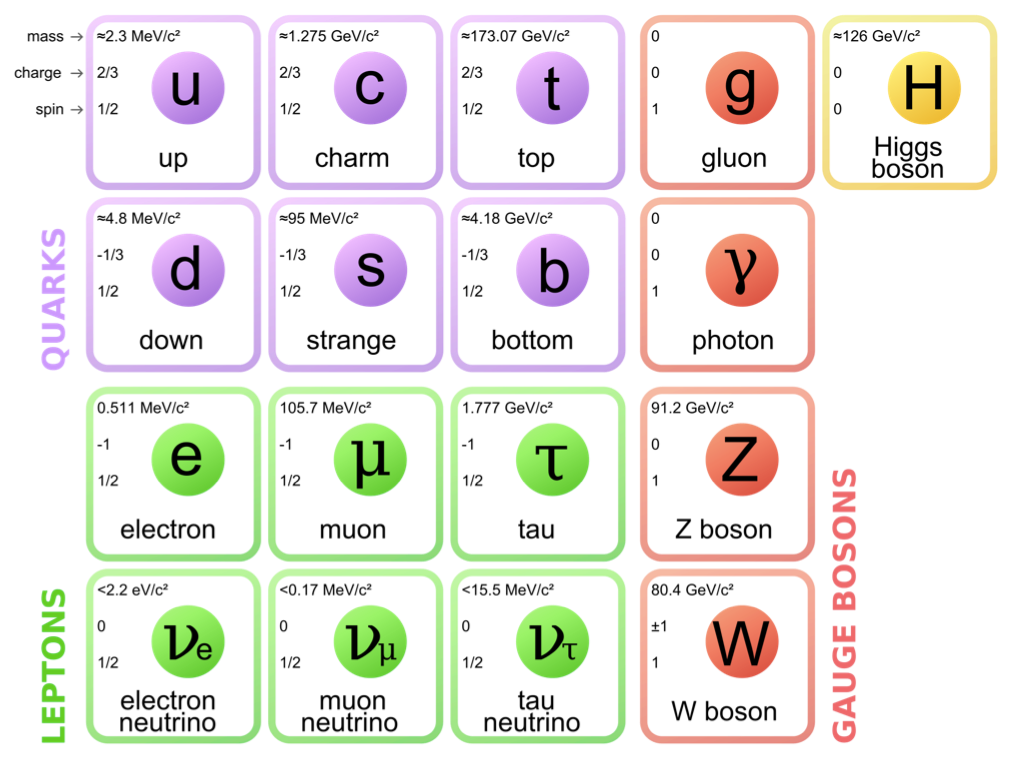
\includegraphics[width=0.8\textwidth]{Introduction/figs/SM.png}
\caption{A scheme of the fundamental particles in the SM with their properties~\cite{SM_particles}.}
\label{fig:SMparticles}
\end{figure}

Due to the asymptotic freedom of the strong interaction quarks cannot be observed in isolation and 
are always combined with other quarks to form color singlets~\cite{Gross:1973id}. Non-fundamental particles
composed of quarks are called hadrons and are classified into two groups: mesons, where the colour singlet
is achieved by the combination of a quark and an antiquark (\quark\quarkbar), and baryons
formed from three quarks (\quark\quark\quark) of different colours.
Recently, in 2014 and 2015 evidence for new states, formed by four and five quarks, was found~\cite{Aaij:2014jqa,Aaij:2015tga}.
%Recently evidence for particles composed by 4 quarks was also found~\cite{}.


\section{The electroweak interaction}
\label{sec:EMandEW}

The electromagnetic interaction is responsible for binding electrons and nuclei
together to form atoms and its mediator is the photon.
%
%,which also sets the range of the EM force to infinity, since this is proportional to the inverse of the mediator mass.
%In fact Heisenberg's Uncertainty Principle tells us that $\Delta E \Delta t > \hbar$, namely virtual particles
%of energy $\Delta E$ are allowed to exist for time intervals inferior to $\Delta t$. Thus, since particles can move
%at most at the speed of light, $c = 299792458$ ms$^{-1}$~\cite{PDG2014}, this also sets a relation between the length 
%of time and space in which a virtual photons can exist ($\Delta t > \hbar / (mc^2)$). As virtual photons can be very
%close to the mass shell, this results in a very long lifetime. The EM force has therefore an infinite range.
%
The weak interaction is responsible for the $\beta$ decay of nuclei and is mediated
by the exchange of $W^\pm$ and $Z^0$ bosons. Unlike the electromagnetic force,
that affects only charged particles, all known fermions interact through the weak interaction.
The weak interaction is also the only one that violates the parity symmetry, which states that interactions are invariant under
an inversion of spatial coordinates. This symmetry breaking arises from the fact that only left-handed fermions interact through
the weak interaction as discovered by Wu in 1957~\cite{Wu:1957my}. Similarly, the weak interaction
is the only one that also breaks the CP symmetry, which combines parity transformations and charge conjugation.
This is particularly interesting because all interactions are believed to be invariant under the CPT transformation, which combines the CP
transformation and time reversal. Hence, breaking CP the weak interaction implies that the process is also not invariant under 
time reversal transformations.

In 1968 Salam, Glashow and Weinberg unified the weak and electromagnetic forces into a single theory, where the coupling
constants of the electromagnetic, $e$, and weak, $g$, interactions are related through the weak mixing angle, $\theta_W$
by the relation $g\sin\theta_W = e$~\cite{PDG2014}. 
%
The electroweak symmetry is spontaneously broken by the Higgs
mechanism~\cite{Strocchi:1977za} and this causes the $W^\pm$ and \Z bosons to become massive (see Tab.~\ref{tab:interactions}) 
and consequently the weak force has a very short range. In fact, using Heisenberg's Principle, $\Delta E \Delta t > \hbar$, 
together with Einstein's formula $\Delta E = m c^2$, which relates mass and energy, and knowing that the maximum 
space that a particle can cover in a time $\Delta t$ is $r \sim c \Delta t$, qualitatively $r \sim \hbar / mc$. In this picture
the carriers of the weak force can travel $r \sim 2 \cdot 10^{-3}$~fm. In contrast, the photon must be massless in the theory, 
which accounts for the long range of the electromagnetic force.
%
The EW interactions are divided into Charged Currents (CC) and Neutral
Currents (NC). In the first group, quarks and leptons interact with the $W^\pm$ bosons, producing decays such as
$\mu^+(\mu^-) \rightarrow e^+ \nu_e \overline{\nu}_\mu (e^- \overline{\nu}_e \nu_\mu)$ and $n (\overline{n}) \rightarrow p e^- \overline{\nu}_e (\overline{p} e^+ \nu_e)$.
The study of these processes confirmed that only the left-handed (right-handed) component of fermions (anti-fermions)
takes part in weak processes. The CC interactions have a peculiarity: they are the only interactions in the SM that violate
flavour conservation at tree level, while any other interaction not conserving flavour has to proceed through
higher order processes. The second group of EW interactions, NC, corresponds to diagrams mediated by a photon or a \Z 
boson interacting with a fermion and its anti-fermion.



\section{Flavour and the CKM matrix}
\label{sec:flavour}

``Flavour" in particle physics refers to the quark/lepton composition of a particle. The introduction of flavour quantum numbers
was motivated in order to explain why some decays, although kinematically allowed, had never been observed. All leptons are
assigned a quantum number $L_\ell = 1$ (where $\ell = e,\mu,\tau$), which in the SM is conserved by all interactions.
This conservation is experimentally well established; for example decays like $\mu^- \rightarrow e^- \gamma $ have never
been observed.
%This is explained by the fact that the lepton number in the initial
%and final state are different and the decay would violate lepton flavour.
%
In the hadronic sector particles carry flavour numbers described as:
%
 \begin{itemize}
 \item \emph{Isospin}: $I_3 = 1/2$ for the up quark and $I_3 = -1/2$ for the down quark;
 \item \emph{Strangeness}: $S = -(n_s - \bar{n}_s)$, where $n_s$ and $\bar{n}_s$ are the numbers of strange
 and anti-strange quarks respectively;
 \item \emph{charmness, bottomness, topness}: in analogy to strangeness
 they are respectively defined as $C = -(n_c - \bar{n}_c)$, $B = -(n_b - \bar{n}_b)$, $T = -(n_t - \bar{n}_t)$.
 \end{itemize}

As mentioned previously, in the SM the only interaction violating flavour conservation is the weak interaction
when mediated by $W^\pm$ bosons.

Measuring branching fractions of weak decays such as $\pi \to \mu \nu_\mu$ and $K \to \mu \nu_\mu$, corresponding
respectively to $ud\to\mu\nu_\mu$ and $us\to\mu\nu_\mu$ processes, suggested the existence of more than one
coupling constant for different quarks. Nicola Cabibbo, in order to preserve the universality
of weak interactions, suggested that the differences could arise from the fact that
the doublets participating in the weak interactions are an admixture of the mass eigenstates~\cite{PDG2014,Cabibbo:1963yz}. 
He therefore introduced the Cabibbo angle, $\theta_c$, proposing that mass eigenstates participating 
in the weak interaction are rotated with respect to the flavour eigenstates.
%
\begin{equation}
\left( \begin{array}{c}
d_W \\ s_W
\end{array} \right) =
\left( \begin{array}{cc}
\cos \theta_c  & \sin \theta_c\\
-\sin \theta_c & \cos \theta_c
\end{array} \right)
\left( \begin{array}{c}
d \\ s
\end{array} \right) = 
\left( \begin{array}{c}
\cos\theta_c \cdot d + \sin \theta_c \cdot s \\
\cos \theta_c \cdot s - \sin \theta_c \cdot d
\end{array} \right)
\end{equation}

In a six quark system one angle is not sufficient to describe a rotation but the mixing can be generalised
using a $3 \times 3$ unitary matrix, called the CKM matrix, from the names of Cabibbo, Kobayashi and Maskawa~\cite{Cabibbo:1963yz,Kobayashi:1973fv}.
The unitarity of the matrix is required to preserve the universality of the weak interaction. Theoretically, a $N \times N$ complex
matrix depends on $2 \cdot N^2$ real parameters. Requiring unitarity ($AA^\dagger = A(A^*)^T = I$), the number
of independent parameters left is 
\begin{equation}
(N - 1)^2 = \underbrace{\frac{1}{2}N(N-1)}_\text{Number of mixing angles} + \underbrace{\frac{1}{2}(N-1)(N-2)}_\text{Number of complex phases}.
\end{equation}  
Therefore a $3 \times 3$ matrix depends then on 4 real parameters: three real constants 
and one imaginary phase. The imaginary phase generates the \mbox{CP-violation} which was
observed in weak interactions.
Figure~\ref{fig:ch_currents_ckm} displays examples of CC processes together with the CKM elements associated with their vertices.
%
\begin{figure}[h!]
\centering 
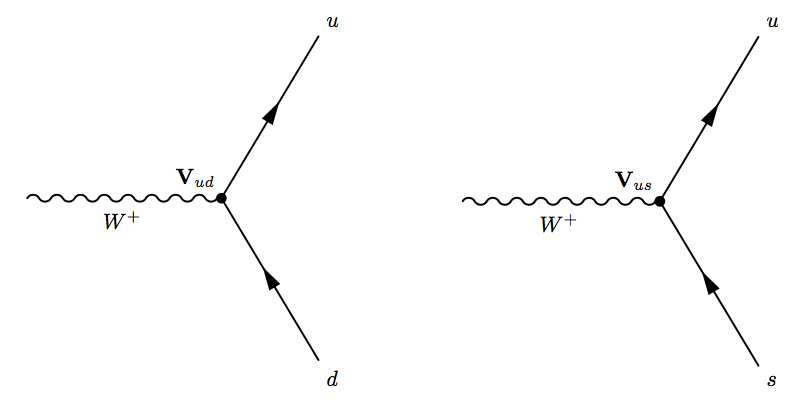
\includegraphics[width=0.6\textwidth]{Introduction/figs/ch_currents_ckm.png}
\caption{Feynman diagrams with CKM weights on weak interaction vertices as defined in Eq.~\ref{eq:CKM}.}
\label{fig:ch_currents_ckm}
\end{figure}
%
Equation~\ref{eq:CKM} reports the most recent measured values of its elements~\cite{PDG2014}
together with the widely used Wolfenstein parameterisation which highlights the hierarchical structure of the matrix.
In fact, elements on the diagonal, corresponding to transitions between quarks of the same generation,
are approximately 1 and become smaller and smaller going farther from the diagonal.
In the formula $\rho$, $A$, and $\lambda$ are the real constants and $\eta$ the imaginary phase 
and Eq.~\ref{params} shows how they are related to the three mixing angles; terms further from the diagonal 
are proportional to higher powers of $\lambda$.
%
\begin{eqnarray}
& V = \left( \begin{array}{ccc}
V_{ud} & V_{us} & V_{ub}  \\
V_{cd} & V_{cs} & V_{cb}  \\
V_{td} & V_{ts} & V_{tb}  
 \end{array} \right) = \left( \begin{array}{ccc}
0.9743 \pm 0.0002 & 0.2253 \pm 0.0007 & 0.0035^{+0.0002}_{-0.001} \\
 0.2252 \pm 0.0007 & 0.9734 \pm 0.0002 & 0.00412^{+0.0011}_{-0.0005} \\
 0.0087 \pm 0.0003 & 0.0404^{+0.0011}_{-0.0005} & 0.99915^{+0.00002}_{-0.00004} 
 \end{array} \right) \nonumber \\ [8pt]
& = \left( \begin{array}{ccc}
1 - \lambda^2/2 & \lambda  & A \lambda^3(\rho -i\eta) \\
-\lambda & 1 - \lambda^2/2 & A\lambda^2 \\
A \lambda^3(1 - \rho -i\eta) & A\lambda^2 & 1 
\end{array} \right) + O(\lambda^4)
\label{eq:CKM}
\end{eqnarray}
%
\begin{equation}
\begin{array}{rl}
\lambda & = \sin(\theta_{12}) = \sin(\theta_c) \\
A\lambda^2 & = \sin(\theta_{23}) \\
A\lambda^3(\rho - i\eta) & = \sin(\theta_{13})e^{i\delta}
\end{array}
\label{params}
\end{equation}
%
%
%Another feature to note is that, due to the unitarity of the matrix, the transformation has no effect on neutral interactions.
%
%In fact defining $q' = Vq$:
%
%\begin{equation}
%\bar{q}'q' = \bar{q}V^{*}Vq = \bar{q}q.
%\end{equation}
%
%As a result flavour-changing neutral currents are forbidden at tree level in the SM.
%

The unitarity of the CKM matrix imposes constraints to its elements of the form:
\begin{equation}
\sum_i |V_{ik}|^2 = 1 \text{ and } \sum_k V_{ik} V^{*}_{jk} = 0.
\end{equation}
These correspond to constraints on three complex numbers, which can be viewed
as the sides of triangles in the $(\rho,\eta)$ plane; these are called ``unitarity triangles".
The most commonly used unitarity triangle arises from $V_{ud}V^*_{ub} + V_{cd}V^*_{cb} + V_{td}V^*_{tb}=0$.
%\begin{equation}
%V_{ud}V^*_{ub} + V_{cd}V^*_{cb} + V_{td}V^*_{tb}=0.
%\end{equation}
Figure~\ref{fig:unitarity_triangle} shows a representation of such triangle together with
a plot summarising the most up-to-date experimental constraints to its parameters~\cite{Charles:2015gya}.
Due to these unitarity constraints flavour-changing neutral currents
are forbidden at tree level in the SM.

The precise measurement of the parameters of the CKM matrix
is a powerful stability test of the SM and sets a solid basis for new physics
searches in the flavour sector. One of the main goals of the LHCb experiment is to measure precisely
 the angle $\gamma$, which is currently the least constrained by measurements.
 %
\begin{figure}[h!]
\centering 
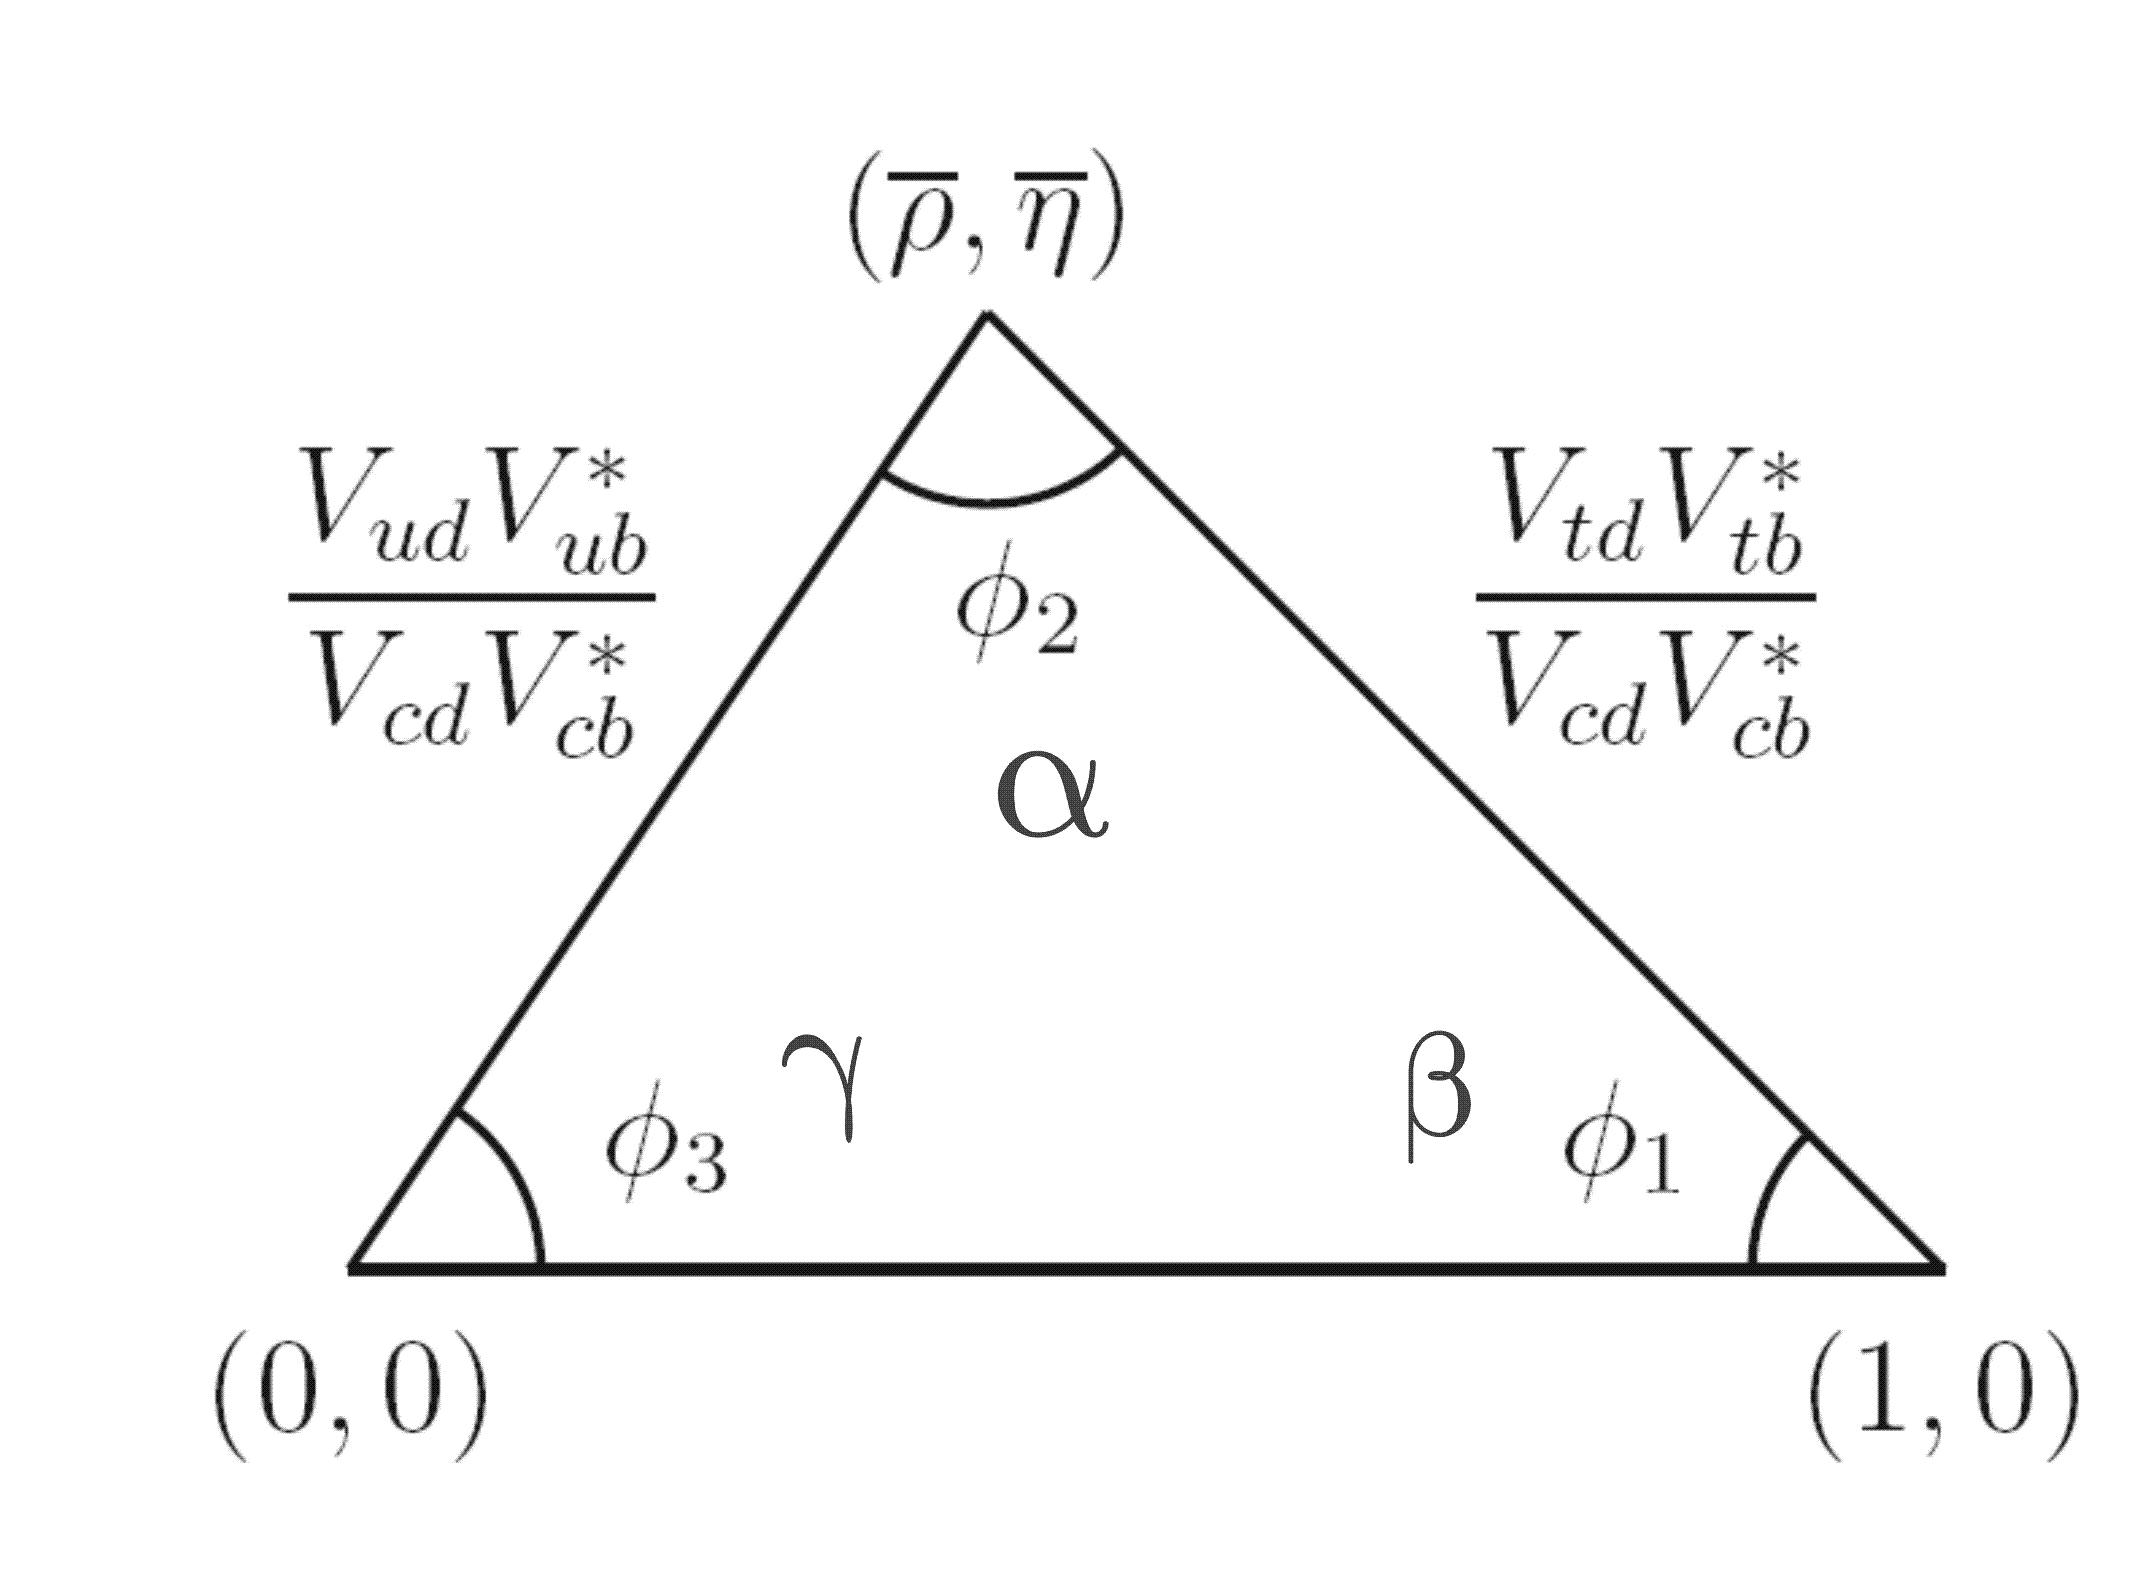
\includegraphics[width=0.5\textwidth]{Introduction/figs/Unitarity_triangle.png}
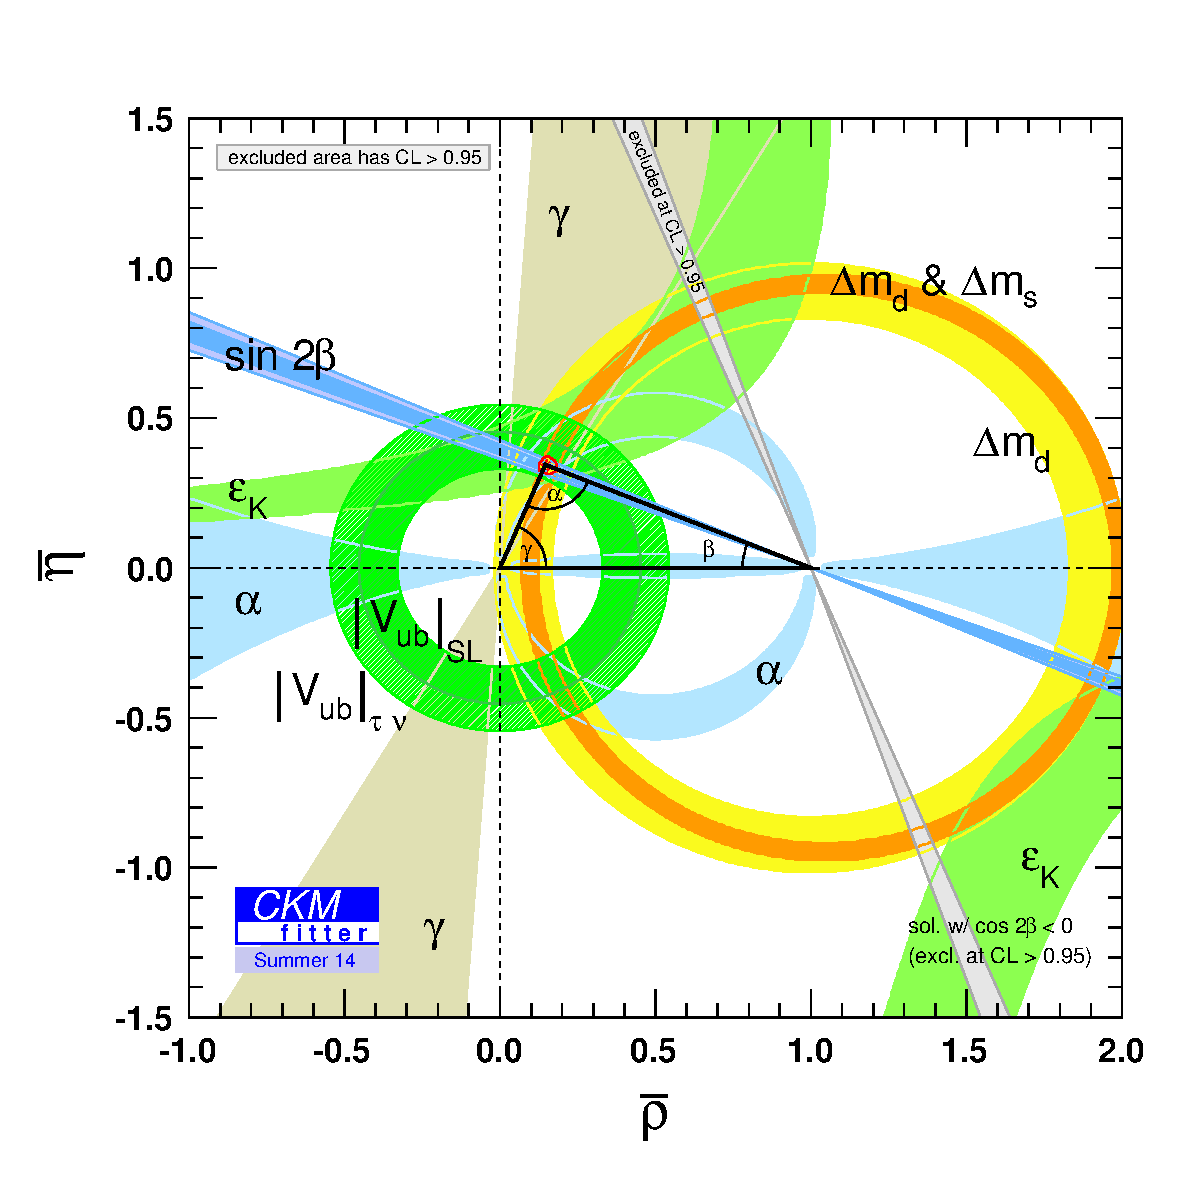
\includegraphics[width=0.7\textwidth]{Introduction/figs/Unitarity_triangle_HFAG.pdf}
\caption{(top) A representation of the unitarity triangle and its parameters.
(bottom) A summary of the most up-to-date measurements of the unitarity triangle parameters~\cite{Charles:2015gya}.}
\label{fig:unitarity_triangle}
\end{figure}
 
 
 
 
\section{The puzzles of the SM}
\label{sec:SMproblems}

Despite the experimental confirmation of many predictions of the SM, the theory has several limitations
and is unable to account for some well-established experimental facts:
%
\begin{itemize}
\item \emph{Dark matter}: experimental evidence tells us that the content of visible matter in the universe is not sufficient
to account for the observed rotation of galaxies~\cite{Zwicky:1933gu}. The most natural way to solve the problem
is the hypothesis of a form of matter that interacts with the gravitational field but not with the other SM interactions. 
%Furthermore, studies of the fluctuations of the cosmic microwave background indicate the existence of
%cold dark matter~\cite{Dunkley:2008ie}.
%formed of particles which do not interact through the SM forces and
%for which there is no SM candidate.
%
\item \emph{Matter-antimatter asymmetry}: a large asymmetry is observed between the quantity of matter 
and antimatter in the universe, $O(10^{-9})$. Assuming that both were equally created in the initial state of 
the universe, a condition such as the violation of the CP symmetry is necessary to account for the observed
imbalance. However, the magnitude of CP violation predicted by the SM, $O(10^{-20})$, is not sufficient to 
account for the observed asymmetry~\cite{Gavela:1993ts}.
%
\item \emph{Gravity}: even though the gravitational force was the first to be discovered 
this is not included in the SM. % as it can be neglected at the EW scale. 
When introducing gravity into the framework of QFT the
theory diverges. On the other hand gravity becomes irrelevant for the small masses 
of particles and can be neglected to a good approximation at the EW energy scale.
Many attempts have been made but there is not yet a consistent theoretical framework through which
 gravity can be introduced in the SM~\cite{Carlip:2001wq}. 
%
\item \emph{Neutrino oscillation}: measurements of solar and atmospheric neutrinos, as well as
neutrinos from nuclear reactors, have established that neutrinos can change flavour while propagating in space.
This is not predicted in the SM, in fact in the SM neutrinos are massless, while an oscillation requires a non-zero
 mass~\cite{Maltoni:2011zz,Cleveland:1998nv,Fukuda:1998mi,Eguchi:2002dm}.
%
\item \emph{The hierarchy problem}: the mass of a scalar (spin 0) particle, such as the Higgs boson,
suffers from quantum corrections due to the physics at high energy scales. As new physics can appear
anywhere up to the Planck scale, $\sim 10^{19}$~\gev, at which gravity cannot be neglected any more,
these corrections can be very large and it would require a high level of fine-tuning for them to cancel 
out and give such a small value as the one measured for the
Higgs Mass, $\sim 126$~\gevcc~\cite{Feng:2013pwa,Aad:2012tfa}. 
%This is considered unnatural by many physicists and pushes them
%to look for further motivations.
%
\end{itemize}
%
In conclusion, even though the SM has been very successful in describing the properties of the observed particles
and their interactions so far, because of its many puzzles, it is believed only to be part of a more general theory 
or only to be valid up to a certain energy scale. %Many theoretical models expect New Physics (NP) to enter at the TeV scale.

\subsection{The flavour problem}

%As mentioned in Sec.~\ref{sec:flavour}, flavour conservation is well experimentally established but it does not
%have a strong theoretical otivation in the Standard Model.
Flavour Changing Charged Currents (FCCC) that are mediated by the $W^\pm$ bosons are the only sources of flavour changing interactions 
in the SM and, in particular, of generation changing interactions, where a quark or a lepton of a family transforms
into one of an other family. Another class of processes is the Flavour Changing Neutral Currents (FCNCs), \emph{e.g.} transitions from a
\bquark quark with a charge of -1/3 to a \squark or \dquark quark with the same charge. Examples of FCNC transitions in the quark
and lepton sector are shown in Fig.~\ref{fig:neutr_curr}.
%
\begin{figure}[h!]
\centering 
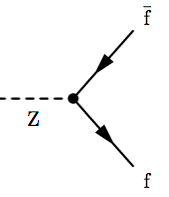
\includegraphics[width=0.25\textwidth]{Introduction/figs/Z2ffbar.png}
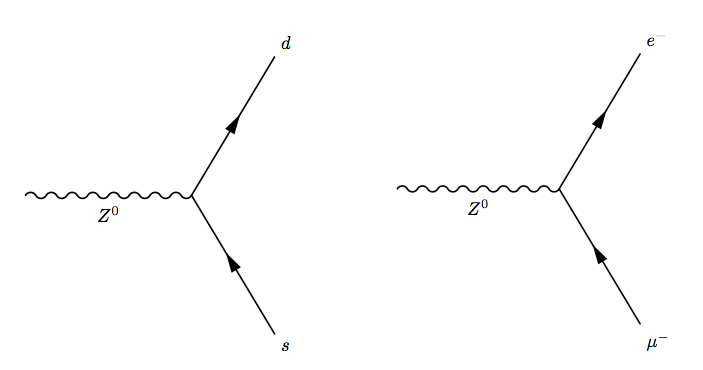
\includegraphics[width=0.6\textwidth]{Introduction/figs/neutral_current_proc.png}
\caption{Feynman diagrams of a neutral current allowed in the SM (left), where$f$ represents any fermion,
and FCNCs processes forbidden in the SM (center-right).}
\label{fig:neutr_curr}
\end{figure}
%
FCNCs are experimentally observed to be highly suppressed which derives from the unitarity of the CKM matrix,
however there is no fundamental reason why there cannot be FCNCs at tree level. In fact the CKM matrix
could be part of a larger matrix involving for example quark-lepton terms. This would introduce
new sources of FCNCs but could also allow for natural explanations of the equality of the proton and electron charges.
Furthermore, the observation of neutrino oscillation proves that flavour is not always conserved
suggesting flavour structures beyond the SM. Finally, the values of the terms of the CKM matrix and the PMNS
matrix~\cite{Pontecorvo:1967fh,Maki:1962mu}, which is the mixing-matrix equivalent to the CKM in the lepton sector,
are not explained in the SM but have to be measured experimentally. These open problems motivate searches for flavour
symmetries and deeper motivations for flavour conservation. 

\section{Beyond the Standard Model}

From the previous sections it is evident that, despite the great success of the SM, there is a need to explore theories Beyond the SM (BSM).
Among the most promising approaches there are those involving Super-Symmetry (SUSY)~\cite{Fayet:1976cr} and extra-dimensions~\cite{Randall:1999ee}. 
%
In SUSY new degrees of freedom are introduced to suppress the diverging terms of the Higgs mass. This theory
assumes that for each fermion there is a corresponding boson and, since bosons and fermions contribute with opposite
sign to the mass term, these would naturally cancel out. Super-Symmetry also provides a candidate for dark
matter. In fact the lightest Super-Symmetric particle, the neutralino, which in R-parity~\cite{Ellis:1984gi} conserving 
variants of the theory must be stable, is a weakly interacting and potentially massive particle.
%
The idea to introduce extra-dimensions was triggered by the fact that gravity is not relevant in particle physics but it would 
be natural if all forces had similar strength. By adding extra dimensions to the normal three spatial dimensions, one can restore 
the strength of gravity, as this could be dispersed by the wider space available.
%
In all these approaches, constraints to masses and couplings must be imposed to maintain
compatibility with the SM at the electroweak scale and the existing experimental observations.

\subsection{Flavour and BSM theories}

Most BSM theories predict processes violating flavour conservation. Therefore, the observation or
non-observation of these processes can give important information about new physics.
BSM theories can be classified according to the amount of flavour violation they introduce.
The first class of models to consider is that with Minimal Flavour Violation (MFV).
These are models in which the only sources of flavour changing transitions are governed by the
CKM matrix and the CKM phase is the only source of CP violation.
This definition is driven by the fact that usually a solution of the hierarchy problem is expected
at the TeV scale, while the very small amount of flavour violation observed in measurements
seems to indicate that the SM would remain valid up to much higher energy scales.
It is therefore assumed that new physics must respect flavour symmetry principles, which also makes these
types of models naturally compatible with the SM. Examples of such models include the MSSM
with minimal flavour violation and the SM with one extra-dimension. Reviews of MFV models
are presented in Refs.~\cite{Isidori:2012ts,Buras:2003jf}.
%
%The MFV hypothesis provides a way to resolve the tension between expectation, driven by naturalness arguments,
%that NP should be at the \tev~scale and limits on FCNC processes that point to much higher scales.
%
A powerful test of MFV is provided by the study of ratios between $\bquark\to\dquark$ and $\bquark\to\squark$
transitions, because their Hamiltonians share the same structure. One particularly important example is the ratio between the 
decay rates of $\Bz$ and $\Bs$ into dimuons~\cite{TomRDreview}, as this is a purely leptonic decay free from hadronic uncertainties.
In the SM such ratios are approximately equal to $|V_{td}/V_{td}| \sim 1/25$, only modified by phase space and hadronic
matrix elements, while they can take very different values in non-MFV models.

In the quest for new physics an important role is also played by simplified models
as an intermediate model building step. Instead of constructing theories valid up to the GUT scale
one can consider simplified models, where the SM is extended by the addition of new degrees of freedom
with a limited number of parameters. Such models are easier to constrain but can nevertheless point
in the right direction to build more complete theories. The choice of the new sector to add can be driven 
by the need to explain existing tensions between measurements and SM predictions or by theoretical prejudice.
%
Two models especially relevant when studying rare decays, which are the main topic of this thesis, are 
$Z'$-penguins and leptoquarks. A $Z'$-penguin is a FCNC process involving a neutral field arising from an extra 
U(1) gauge symmetry, for example U(1)$_{B-L}$, where $B$ and $L$ are the baryon and lepton numbers. 
As for the SM penguins, the $Z'$ field contributes in loops causing modifications of the 
effective couplings with respect to the SM. A survey of $Z'$ models can be found in Ref.~\cite{Buras:2014zga}.
%
Leptoquarks are bosonic particles that carry both quark and lepton flavour quantum numbers, which
for simplicity are assumed to be scalar.
A tree level exchange of a leptoquark induces processes such as $\bquark \to (\squark,\dquark)\ell^+\ell^-$,
and therefore can result in an enhancement of their decay rates with respect to the SM~\cite{Hiller:2014yaa}.
Leptoquarks would also provide a natural explanation for non-universal couplings to leptons.


\section{Rare decays: a tool to search for new physics}
\label{sec:RD_theory}

In the Standard Model FCNC processes are forbidden at tree level but
can occur through loop diagrams such as penguin or \W box diagrams (see Fig.~\ref{fig:penguins}).
The branching fractions of decays going through these processes are small, typically \mbox{$\sim10^{-6}$} 
or lower, and therefore they are called ``rare decays". Additional contributions to the virtual loops
are not necessarily suppressed with respect to the SM component which makes these decays
very sensitive to new physics. This approach to new physics searches is interesting as
new particles could be at high mass scales that are not accessible via direct production at colliders
but their effect could be observed in loops.
Radiative and penguin decays are particularly interesting because they are theoretically
well understood, which allows precise comparisons with measurements. Furthermore, they provide
a large quantity of observables that can be affected by new physics, not only decay rates, but also 
CP asymmetries and angular observables such as forward-backward asymmetries. The joint
analysis of different observables can help to build a consistent picture and rule out specific models.
%
\begin{figure}[h!]
\centering
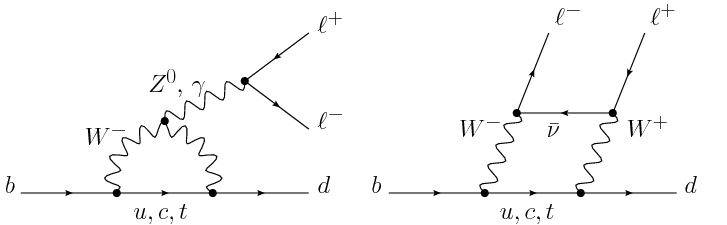
\includegraphics[width=0.9\textwidth]{Introduction/figs/penguin_general.png}
\caption{Loop Feynmann diagrams allowing $\bquark \to \dquark$ FCNC 
processes: penguin diagram (left) and \W box (right).}
\label{fig:penguins}
\end{figure}

\subsection{Theoretical framework: the effective Hamiltonian}
\label{sec:Effective_Hamiltonian}

Rare decays of \bquark hadrons are governed by an interplay between weak
and strong interactions.
%The QCD corrections that arise from hard gluon exchange bring large logarithms
%of the form $\alpha_s^n(m_b)\log^m(m_b/M)$, where $M = m_t$ or $M = m_W$.
%A suitable framework to achieve the necessary resummation of these logarithms
%in an effective low-energy theory with five quarks.
%The QCD corrections that arise from hard gluon exchange bring large contributions
%large logarithms of the form $\alpha_s^n(m_b)\log^m(m_b/M)$, where $M = m_t$ or $M = m_W$.
The large masses of the $W^\pm$ and $Z^0$ bosons and top quark compared to that of the \bquark quark allow
the construction of an effective theory that divides the problem of calculating
weak decay amplitudes into two parts: ``short-distance" and ``long-distance" effects separated
at an energy scale $\mu$. The first part, dealing with short distance physics, handles
perturbative contributions due to energy scales above the \bquark mass. The second part
typically deals with non-perturbative contributions. 
A classic example of an effective theory is the Fermi theory of weak interactions
which describes the $\beta$ decay in terms of a four-fermion interaction,
where the short distance physics is hidden into a point-like vertex as illustrated in Fig.~\ref{fig:fermi_theory}.
\begin{figure}[h!]
\centering
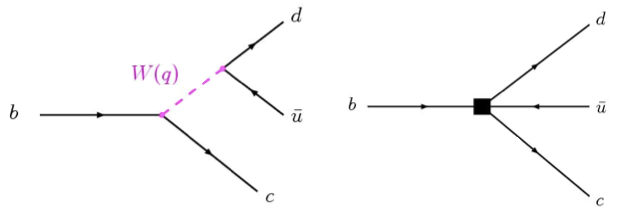
\includegraphics[width=0.7\textwidth]{Introduction/figs/fermi_theory.png}
\caption{Example of a Fermi theory in which the full theory (left) is divided into (right) a
short distance contribution, hidden in the vertex, and a long distance contribution.}
\label{fig:fermi_theory}
\end{figure}
\clearpage
The effective Hamiltonian~\cite{Chetyrkin:1996vx} relevant to
$\bquark\to\squark/\dquark \gamma$ and  $\bquark\to\squark/\dquark \ell^+\ell^-$
transitions can be written as:
%
\begin{equation}
\mathcal{H}_{eff} = \frac{-4G_F}{\sqrt{2}} \left[ \lambda^t_q \sum C_i(\mu,M)\mathcal{O}_i(\mu)
+ \lambda^u_q \sum C_i(\mu,M)(\mathcal{O}_i(\mu) - \mathcal{O}_i^u(\mu)) \right],
\end{equation}
%
where $G_F$ denotes the Fermi coupling constant and the $\lambda$ constants are the CKM factors,  
$\lambda^t_q = V_{tb}V_{tq}^*$ and  $\lambda^u_q = V_{ub}V_{uq}^*$. In $\bquark\to\squark$ quark transitions, 
which are the main topic of this thesis, the doubly Cabibbo-suppressed contributions can be neglected as 
$\lambda^u_s << \lambda^t_s$. To obtain this formula the Operator Product Expansion (OPE)~\cite{Buchalla:1995vs} method
is used, which implements a summation over all contributing operators weighted by corresponding constants
called Wilson coefficients. In this Hamiltonian the long-distance contributions are described by the 
operators, $\mathcal{O}_i$, while the short-distance physics is encoded in the Wilson 
coefficients, $C_i$. Operators and coefficients are evaluated at the renormalisation scale $\mu$.
Any particle that contributes to the decay and has a mass greater than the scale $\mu$ will affect the value 
of at least one of the Wilson coefficients, including SM particles as the top quark.

In order to describe SM processes the effective theory must be matched with the SM by requiring 
the equality between each term in effective theory and the full theoretical calculation at a matching 
scale, typically the EW scale ($\mu_W$). Then, using the scale independence of the
effective Hamiltonian, one can derive a renormalisation group equation for the Wilson coefficients~\cite{Buras:1998raa}.
%
%
%\begin{equation}
%\mu \frac{\deriv}{\deriv \mu} C_i(\mu) = \gamma_{ij}C_j(\mu),
%\end{equation}
%
%where the matrix $\gamma$ is the anomalous dimensions matrix of the operators $\mathcal{O}_i$.
%At leading order the solution is given by~\cite{Buras:1998raa}:
%
%\begin{equation}
%C_i(\mu) = \left[ \frac{\alpha_s(\mu_W)}{\alpha_s(\mu)}\right]^{\frac{\gamma^0_{ii}}{2\beta_0}} C_i(\mu_W) = \left[ \frac{1}{1 + \beta_0\frac{\alpha_s(\mu)}{4\pi}ln\frac{\mu_W^2}{\mu^2}} \right]^{\frac{\gamma^0_{ii}}{2\beta_0}} C_i(\mu_W),
%\end{equation}
%
%where $\alpha_s$ is the strong coupling constant.
%
Taking into account only SM contributions and using $\mu_W = m_b$, the Wilson coefficients have values:
%
\begin{equation}
\begin{array}{ccc}
C_7^{SM} = -0.3, & C_9^{SM} = 4.2, & C_{10}^{SM} = -4.2
\end{array}
\end{equation}
%
and new physics contributions appear in the Wilson coefficients in the form of additive factors:
\begin{equation}
 C_i = C_i^{NP} + C_i^{SM}.
\end{equation}

The amplitudes of exclusive hadronic decays can be calculated as the expectation 
values of the effective Hamiltonian. Given an initial state $I$ and a final state $F$
\mbox{(\emph{e.g.}: $I = \Bz$ and $F=\Kstarz\mumu$)} the decay amplitude can be calculated as
%
\begin{equation}
\begin{array}{rl}
A(I\to F) &= \langle I | \mathcal{H}_{eff} | F \rangle = \\
&= \frac{G_F}{\sqrt{2}} \sum V_{CKM}^i \underbrace{C_i(\mu)}_{\shortstack{Perturbative \\ Includes new physics}} \cdot  \underbrace{\langle I | \mathcal{O}_i(\mu) | F \rangle}_{\shortstack{Non-preturbative \\ Known physics}},
\end{array}
\end{equation}
where $\langle I | \mathcal{O}_i(\mu) | F \rangle$ are the hadronic matrix elements also called  ``form factors".
These can be evaluated using non perturbative methods such as lattice calculations.
However, due to the limitations of these methods, they represent the dominant source 
of uncertainty in theoretical calculations.

\subsection{Operators}
\label{sec:operators}

Separating the left- and right-handed components the effective Hamiltonian is
%for $\bquark\to\squark\ell^+\ell^-$ transitions is
%
\begin{equation}
\mathcal{H}_{eff} = \frac{4G_F}{\sqrt{2}} V_{tb}V^*_{ts} \frac{\alpha_e}{4\pi} \sum_{i=1}^{10} \left[ C_i \mathcal{O}_i  +  C'_i \mathcal{O}'_i \right].
\end{equation}
%
%where the $V_{ub}$ and $V_{bs}$ are the factors of the CKM matrix.
A complete basis is given by a set of 10 operators, where $\mathcal{O}_{1,2}$ are the tree level W operators;
$\mathcal{O}_{3-6,8}$ are penguin diagrams mediated by gluons; and $\mathcal{O}_{7,9,10}$, which are the operators
that are relevant for radiative and leptonic penguin processes are defined as~\cite{TomRDreview}:
%S is Higgs scalar penguins and P pseudo-scalar penguin
%
\begin{equation}
\begin{array}{ll}
 \mathcal{O}_7 = \frac{m_b}{e} (\bar{s} \sigma^{\mu\nu}P_Rb)F_{\mu\nu},  		& \mathcal{O}_7' = \frac{m_b}{e} (\bar{s} \sigma^{\mu\nu}P_Lb)F_{\mu\nu}, \\
%\mathcal{O}_8 = g_s\frac{m_b}{e} (\bar{s} \sigma^{\mu\nu}P_RT^ab)G^a_{\mu\nu}  	& \mathcal{O}_8' = g_s\frac{m_b}{e} (\bar{s} \sigma^{\mu\nu}P_LT^ab)G^a_{\mu\nu} \\
\mathcal{O}_9 = (\bar{s} \gamma_{\mu}P_Lb)(\bar{\ell}\gamma^\mu\ell), 			& \mathcal{O}_9' = (\bar{s} \gamma_{\mu}P_Rb)(\bar{\ell}\gamma^\mu\ell), \\
\mathcal{O}_{10} = (\bar{s} \gamma_{\mu}P_Lb)(\bar{\ell}\gamma^\mu\gamma_5\ell), 	& \mathcal{O}_{10}' = (\bar{s} \gamma_{\mu}P_Rb)(\bar{\ell}\gamma^\mu\gamma_5\ell),
\end{array}
\end{equation}
%
where $P_{L/R} = (1 \mp \gamma_5)/2$ denote the left- and right-handed chiral projections 
%$T^a$ are the QCD generators 
and $F_{\mu\nu}$ is the electromagnetic field tensor.
%
The $\mathcal{O}'$ operators correspond to right-handed coupling obtained by swapping
$P_R$ and $P_L$ in the equations. In the SM, as well as in MFV models where the
flavour violation is entirely ruled by the CKM matrix, the $C'$ Wilson coefficients 
are suppressed by the strange coupling, $C'_i \sim (m_s / m_b) C_i$.
%
The operator $\mathcal{O}_7$ relates to penguin diagrams that are mediated via a photon.
%and the $\mathcal{O}_8$ by a gluon. The $\mathcal{O}_7$ operator is 
It represents the dominant contribution to the radiative 
$\bquark\to\squark\gamma$ transition and contributes to $\bquark\to\squark\ell^+\ell^-$ processes when
the virtual photon decays into a dilepton pair. The semileptonic $\mathcal{O}_9$ and $ \mathcal{O}_{10}$ 
correspond to penguin diagrams mediated by a $Z^0$ boson and $W$ mediated box diagrams. 
These are the dominant contributions in semileptonic $\bquark\to\squark\ell^+\ell^-$ decays.
The vertices corresponding to the radiative and semileptonic operators are illustrated in Fig.~\ref{fig:vtx_operators}
%
\begin{figure}[h!]
\centering
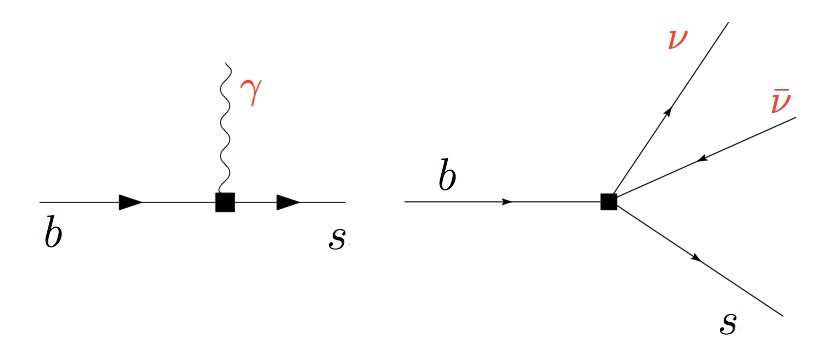
\includegraphics[width=0.6\textwidth]{Introduction/figs/vtx_operators.png}
\caption{Interaction vertices corresponding to the radiative (left) and semileptonic (right) operators.}
\label{fig:vtx_operators}
\end{figure}

It is also common to express the semileptonic operators in a basis with left and right projected leptons
%
\begin{equation}
\begin{array}{ll}
\mathcal{O}_{LL} = ( \mathcal{O}_{9} - \mathcal{O}_{10})/2 & \mathcal{O}_{LR} = ( \mathcal{O}_{9} + \mathcal{O}_{10})/2 \\
\mathcal{O}_{RR} = ( \mathcal{O}'_{9} - \mathcal{O}'_{10})/2 & \mathcal{O}'_{RL} = ( \mathcal{O}'_{9} + \mathcal{O}'_{10})/2 \\
\end{array}
\end{equation}
%
where the Wilson coefficients are redefined as
\begin{equation}
\begin{array}{ll}
C_{LL} = C_{9} - C_{10}, & C_{LR} =  C_{9} + C_{10}, \\
C_{RR} = C'_{9} - C'_{10}, &C'_{RL} =  C'_{9} +C_{10}. \\
\end{array}
\end{equation}
%
This basis is particularly useful in frameworks where BSM physics at a high mass scale
respects the SU(2)$_W$ part of the SM gauge symmetry group.
%For instance, instead of fitting the two parameters $C_9$
%and $C_{10}$, the LL-hypothesis gives the constraint $C_9 + C_{10} = 0$.
%since C9 +C10 = 0 in the standard model there is no sensitivity to CLR and 
%CRR from interference with the standard model in semileptonic decays.
%
Finally, in the picture presented in this section all operators were considered as universal
with respect to the flavour of the involved leptons. However, BSM models often contain sources of
lepton universality violation leading to a split of the same operators depending on the lepton considered:
$C_i \to C_i^e$, $C_i^\mu$, $C_i^\tau$ and $\mathcal{O}_i \to \mathcal{O}_i^e$, $\mathcal{O}_i^\mu$, $\mathcal{O}_i^\tau$. 

\subsection{Phenomenology of $\bquark\to\squark\ell^+\ell^-$ decays}
\label{sec:theo_qsq}

Semileptonic \bquark hadron decays are characterised by two kinematic regimes which
are treated theoretically in different ways; Table~\ref{tab:q2scheme} shows a scheme of the \qsq spectrum.
%
The ``high $q^2$" is the region of low hadron recoil, $\qsq > 15$~\gevgevcccc, and is characterised by 
the energy of the hadron being less than the energy scale of QCD interactions within the meson, 
\mbox{$\Lambda_{QCD} \sim 1$~\gev}. In this region theoretical calculations of $B$ meson decays can be simplified 
by working in the heavy quark limit, $m_b\to\infty$. In this limit a Heavy Quark Effective 
Theory (HQET) can be constructed~\cite{DellaMorte:2015yda} in which the heavy quark interacts 
only via `soft' hadronic processes and an OPE in $1/m_b$ is valid.
%?QCD/mb then shows that the perturbatively calculable parton-level process is the leading 
%contribution to the B0 ?K?0?+?? decay, and the hadronic effects are relatively small. 
%. A heavy-quark expansion in terms of The QCD Factori- sation (QCDF) technique separates the parton-level and %hadronic contributions at the energy scale ??mb, accounting for the ?soft? non-perturbative processes using hadronic %form factors [25].
%
%
%\begin{table}[b]
%\caption{A scheme of the \qsq spectrum.}
%\begin{tabular}{llcrr}
%{\footnotesize $\qsq = 0$ }   &  {\footnotesize  $E_{\Kstarz}  >> \Lambda_{QCD}$	}&  {\footnotesize $\qsq \sim m_{\jpsi,\psitwos}^2$ } & {\footnotesize $E_{\Kstarz}  \sim \Lambda_{QCD}$ } & {\footnotesize $\qsq = (m_B - m_\Kstarz)^2$ } \\
%\hline
%{\footnotesize max. recoil } & {\footnotesize large recoil (SCET) } & {\footnotesize $\cquark\cquarkbar$ resonances } & {\footnotesize low recoil (HQET) } & {\footnotesize zero recoil} \\
%\end{tabular}
%\label{tab:q2scheme}
%\end{table}
\begin{table}[b]
\caption{A scheme of the \qsq spectrum.}
\centering
\begin{tabular}{c|c|c|c}
 \qsq							& $E_{\Kstarz}$	   	&  	Regime 			& 	Valid theory \\ \hline
 $\sim 0$ \gevgevcccc			& $\sim m_B$			&   Max. recoil			&	\multirow{ 2}{*}{SCET}\\ 
 $< 6$	\gevgevcccc			& $>> \Lambda_{QCD}$	&	Large recoil		&		   		\\ \hline
 $\qsq \sim m_{\jpsi,\psitwos}^2$ 	& $\sim 3$ \gev			& 	$\cquark\cquarkbar$ resonances	&  -- 		\\ \hline
 $\qsq > 15$ \gevgevcccc 			& $E_{\Kstarz}  \sim \Lambda_{QCD}$ 			&	Low recoil	&	\multirow{ 2}{*}{HQET}\\
 $\qsq = (m_B - m_\Kstarz)^2$ 		& $E_{\Kstarz} \sim 0$  	&	Zero recoil		&			\\
\end{tabular}
\label{tab:q2scheme}
\end{table}
%
The \mbox{``low $q^2$"} region is where the light spectator quark is energetic and cannot be neglected.
Furthermore, the light quark interacts not only via `soft' hadronic processes, as in HQET, but also via the 
so-called `collinear' hadronic processes.
The boundary of this region can be set at $\sim 7$~\gevgevcccc~ which corresponds to the threshold for 
$\cquark\cquarkbar$ production, $(2m_c)^2$. 
In this region the hadronic interactions are handled by expanding in terms 
of the energy of the emitted energetic hadron, $1/E_h$, forming the so-called Soft-Collinear 
Effective Theory (SCET)~\cite{Bauer:2000yr}.
%
\begin{figure}[h!]
\centering
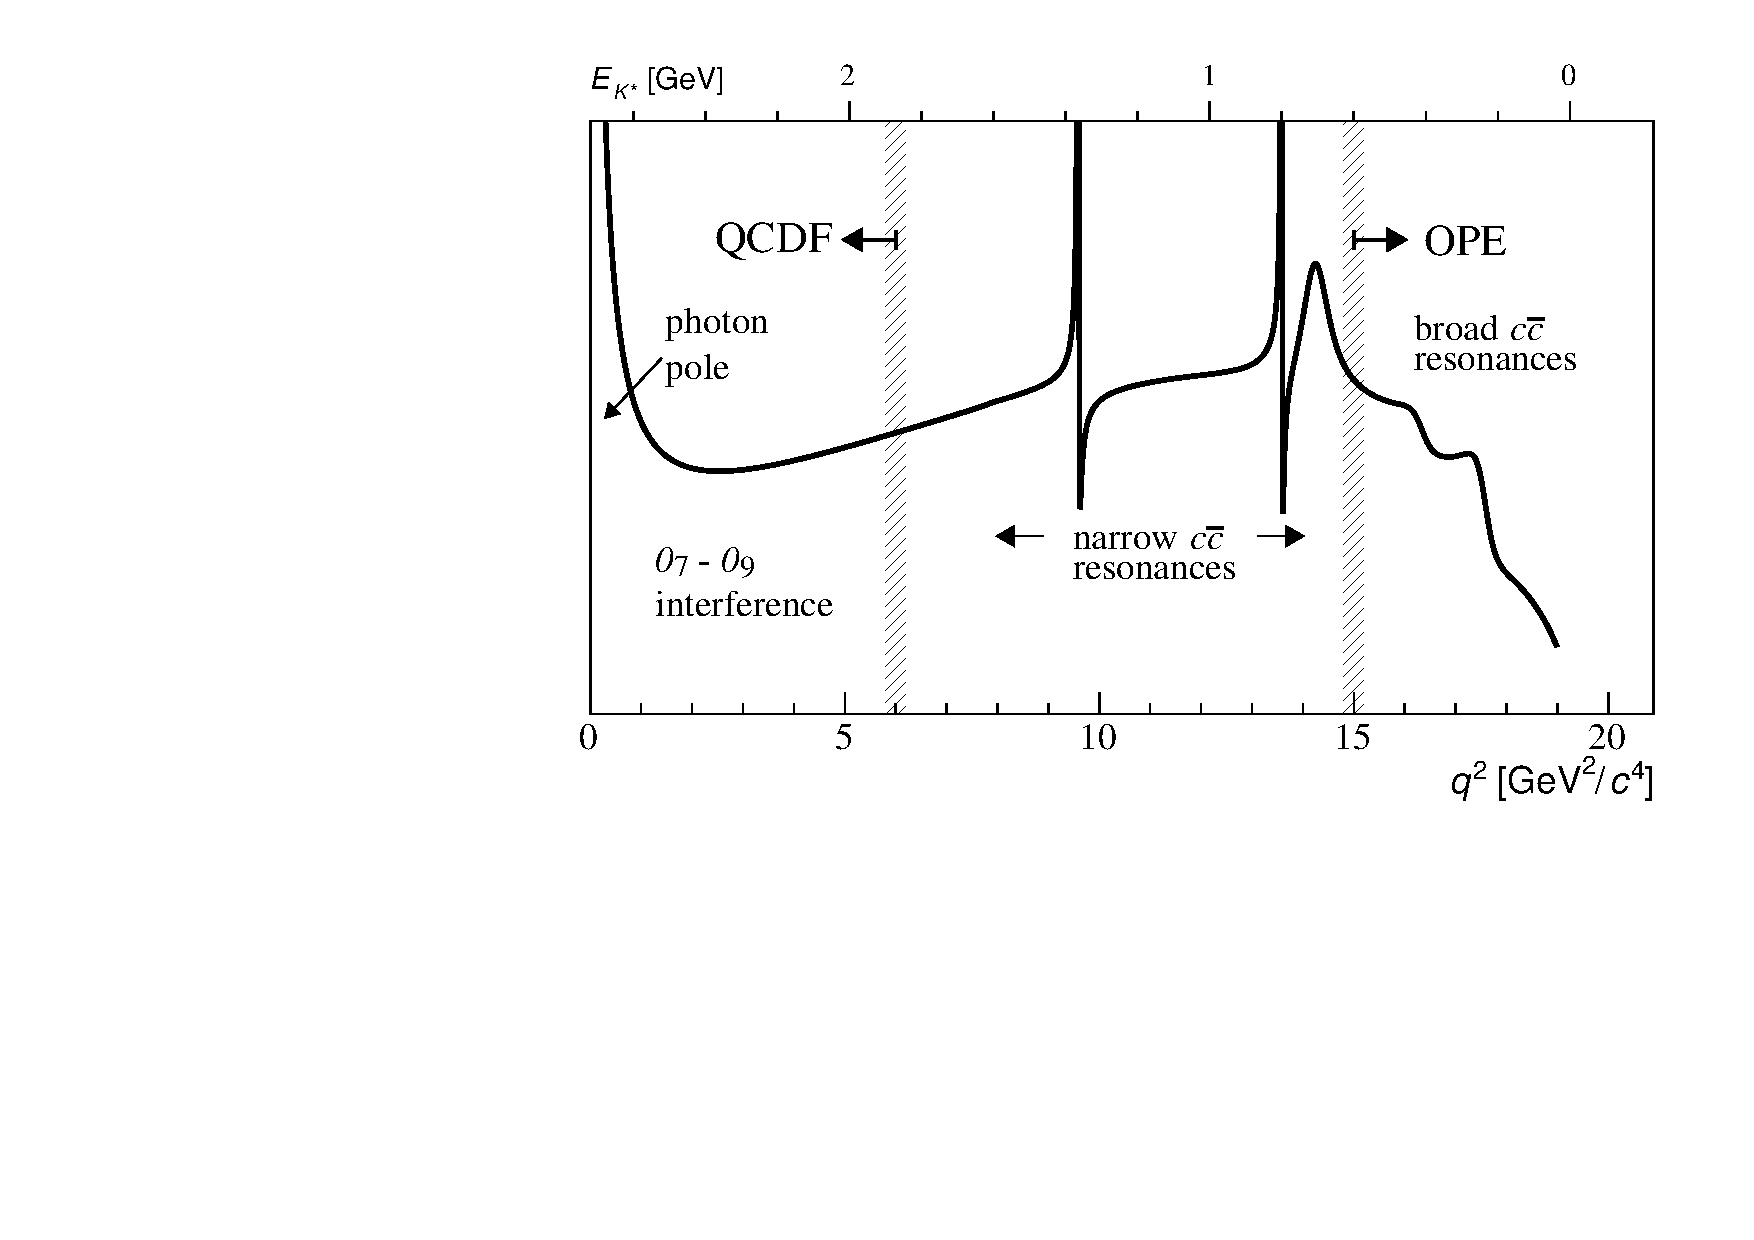
\includegraphics[width=0.8\textwidth]{Introduction/figs/q2spectrum.pdf}
\caption{A typical \qsq spectrum of $\bquark\to\squark\ll$ processes characterised by the photon pole
at  low \qsq, charmonium resonances at central \qsq and broad resonances at high \qsq~\cite{TomRDreview}.}
\label{fig:q2spectrum}
\end{figure}
%
In both regions decay rates can be predicted using the different methods and
the biggest uncertainties come from the limited knowledge of hadronic transition matrix elements.
The intermediate region is characterised by the presence of charmonium resonances, produced though tree 
level $b\to\cbar c s$ transitions and no precise theoretical calculation is available~\cite{Khodjamirian:2010vf}.

As can be seen in Fig.~\ref{fig:q2spectrum} the very low \qsq region is characterised by a peak due
to the virtual photon contribution, associated with $C_7$. In the region $1-6$~\gevgevcccc the 
interference between $C_7$ and $C_9$ becomes large, yielding sensitivity to new physics in $C_9$.
The $7-15$~\gevgevcccc interval is dominated by the charmonium resonances, \jpsi and \psitwos. 
Although these decays can be experimentally vetoed, in
principle charmonia affect the entire \qsq space. Finally, at high \qsq broad charmonium resonances 
can contribute, like those observed by LHCb in $\decay{B^+}{K^+\mumu}$ decays~\cite{LHCB-PAPER-2013-039}.

\subsection{Observables in $\bquark\to\squark\ell^+\ell^-$ decays}
\label{sec:observables}

Rare decays and especially semileptonic $\bquark\to\squark\ell^+\ell^-$ processes offer a number
of observables which can be used to study BSM models.
The most direct effects appear in decay rates that can be enhanced by new physics but the precision on
these measurements is often limited by uncertainties on the non-perturbative part of the calculations.
Therefore, it is important to also look for different observables.
One important class of observables are angular quantities that can often carry complementary 
information with respect to branching ratio measurements. The most basic of these
observable are forward-backward asymmetries that characterise the angular distribution of final particles. 
For the $\Bz\to\Kstarz\mumu$ decay combinations of observables have been proposed
that are independent of form factor uncertainties at leading order order~\cite{TomRDreview}.

Another way to build safe observables is to construct ratios between similar
decays, in which uncertainties due to the hadronisation process cancel out.
These observables include the $R_H$ ratios, between \Bz decays into electrons and muons,
that are described in detail in Ch.~\ref{sec:RKst_theory}.
It is also interesting to compare decays which proceed via the same fundamental process but
where the spectator quark has a different flavour. This is the case of $\Bu\to K^+\mumu$ and $\Bz\to\KS\mumu$
decays, which are both $\bquark\to\squark$ transitions where the spectator quark is a \uquark quark
in the first case and a \dquark quark in the second. The normalised difference of the branching fractions
of these decays is called isospin asymmetry.


\section{Experimental status}
\label{sec:exp_status}

To set the background for the analyses described in this thesis, this section gives a 
brief review of recent results of new physics searches involving rare decays or lepton flavour violation.
Among these, results recently obtained by the \lhcb experiment show a series of anomalies
with respect to the SM that have the potential to yield to BSM scenarios.


\subsection{Dimuon decays of \bquark hadrons}

Decays of $B$ mesons into a pair of muons are two-body decays where the two muons are back to
back in the hadron rest frame. The simple signatures of these decays makes them easy to study
and the fact that they are unaffected by hadronic physics in the final state makes predictions very
clean and precise. Therefore these are essential tests of the SM.
The $\decay{\Bz}{\mumu}$ and $\decay{\Bs}{\mumu}$ decays are FCNCs that can only happen 
via loops and furthermore they are CKM-suppressed, which makes them particularly rare.
In addition, the decay of a pseudo-scalar $B$ meson into two muons has a significant helicity
suppression. The latest SM predictions for these decay rates are~\cite{Bobeth:2013uxa}:
%
\begin{align}
\mathcal{B}(\decay{\Bs}{\mumu}) &= (3.65 \pm 0.23) \times 10^{-9} \text{ and } \\
\mathcal{B}(\decay{\Bz}{\mumu}) &= (1.06 \pm 0.09) \times 10^{-10}.
\end{align}
%
The uncertainties on these values are dominated by the knowledge of the decay constants and 
CKM-elements. BSM models can produce significant enhancement to these decay rates
and the measurement of their ratio is a stringent test of the MFV hypothesis.
A combination of the \lhcb and \cms results gives the values~\cite{CMS:2014xfa}:
%
\begin{align}
\mathcal{B}(\decay{\Bs}{\mumu}) &= (2.8^{+0.7}_{-0.6}) \times 10^{-9} \text{ and } \\
\mathcal{B}(\decay{\Bz}{\mumu}) &= (3.9^{+1.6}_{-1.4}) \times 10^{-10}.
\end{align}
%
%
Neither decay had been previously observed, while now the $\Bs$ decay is observed
with a significance of $6\sigma$ and evidence for the $\Bz$ decay is found
at $3\sigma$ significance level. The measured branching fractions are compatible 
with SM predictions within $2\sigma$ and put strong constraints on the available 
parameter-space for BSM theories. Figure~\ref{fig:bsmumu} shows the fit the dimuon 
invariant mass of $B$ meson candidates where the peaks of the two decays are visible.
%
\begin{figure}[b!]
\centering
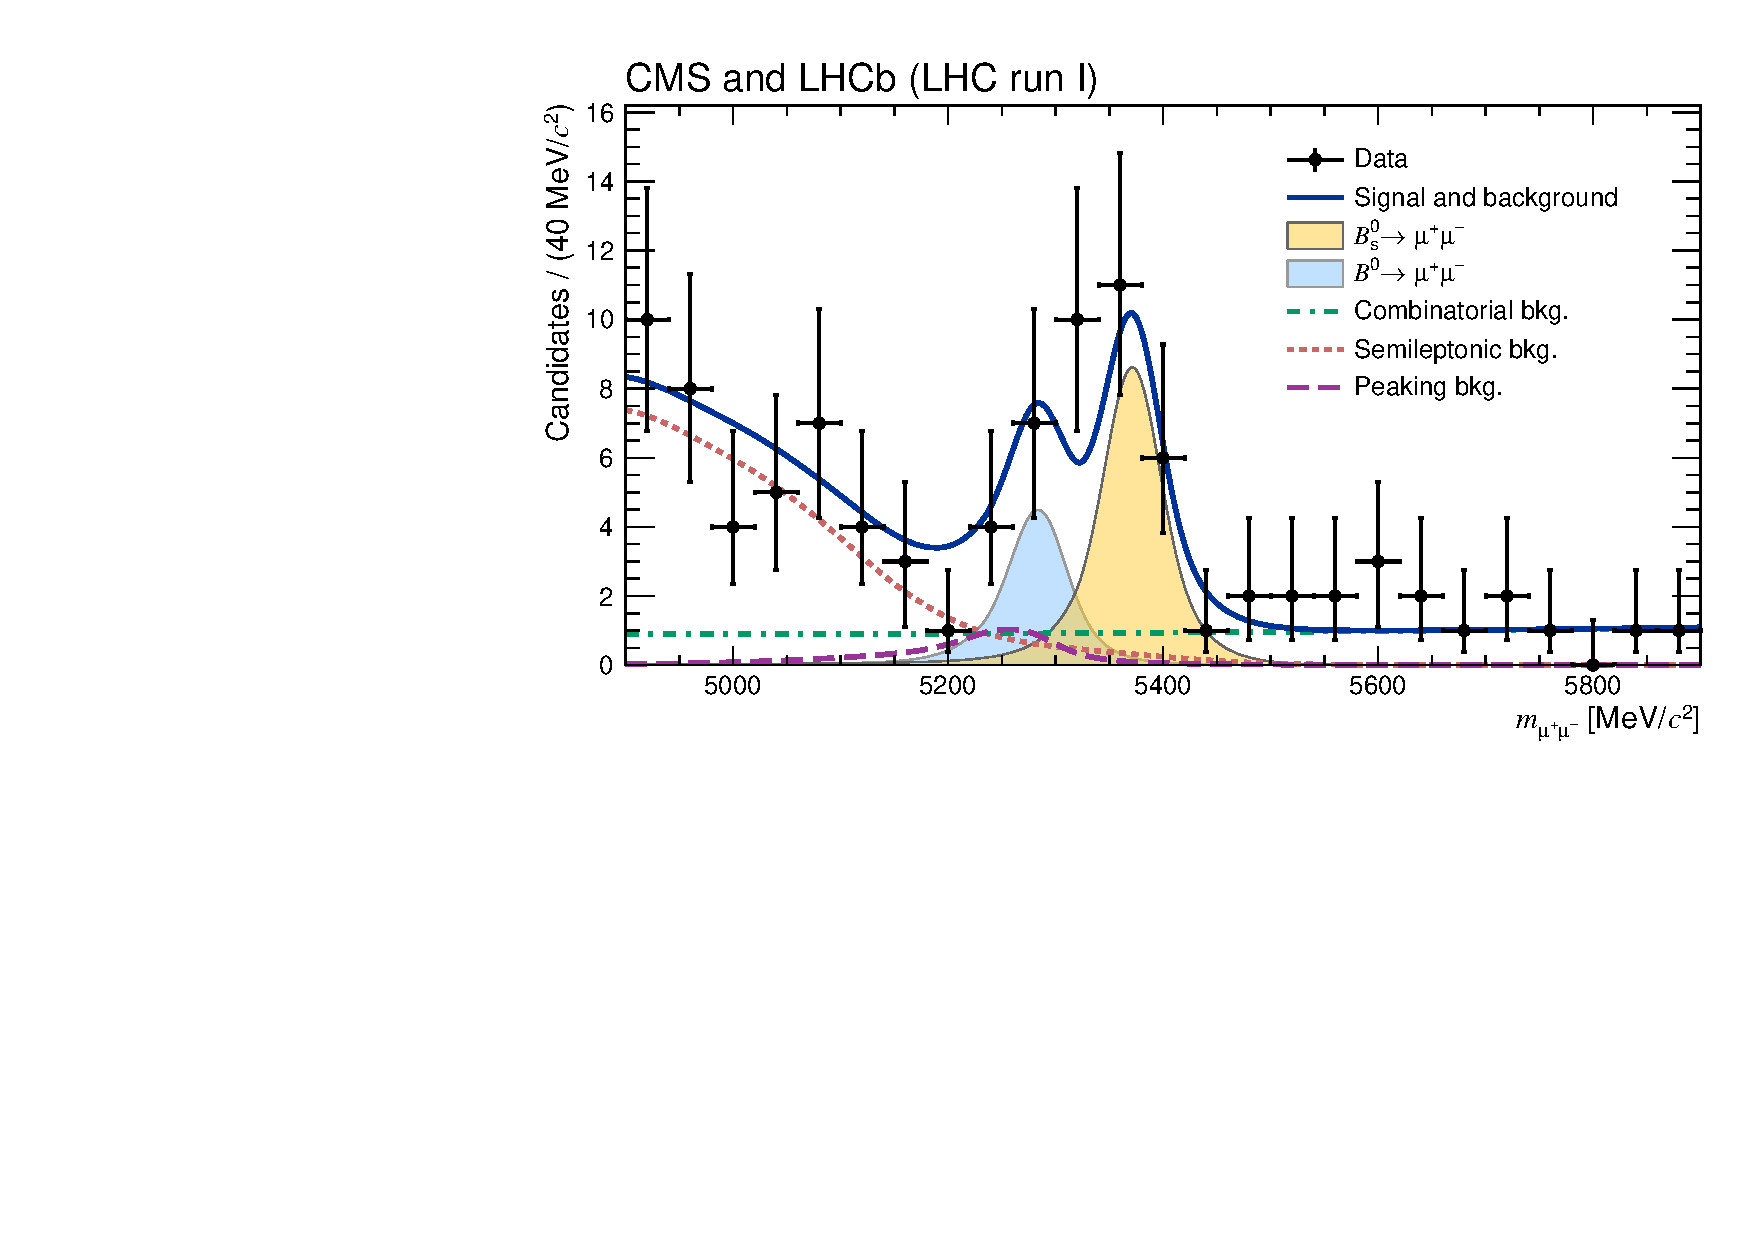
\includegraphics[width=0.6\textwidth]{Introduction/figs/CMSLHCb_EDfig2.pdf}
\caption{Dimuon invariant mass of $B$ candidates showing peaks corresponding 
$\Bs\to\mumu$ and $\Bz\to\mumu$ decays~\cite{CMS:2014xfa}.}
\label{fig:bsmumu}
\end{figure}

\subsection{Semileptonic $\bquark\to\squark\ell^+\ell^-$ decays of \bquark hadrons}
\label{sec:exp_btosll}

At the LHC it is possible to collect large data samples of semileptonic 
decays, especially those with muons in the final state.
Many branching fractions of semileptonic $B$ meson decays were recently measured at
the \lhcb experiment, including $\decay{B}{K\mumu}$, $\decay{B}{\Kstarz\mumu}$
and $\decay{\Bs}{\phi\mumu}$~\cite{LHCB-PAPER-2014-006,LHCB-PAPER-2013-017,LHCB-PAPER-2013-019}. 
Baryon decays were also studied at \lhcb: including 
the rare $\decay{\Lambda_b}{\Lz\mumu}$ decay~\cite{Aaij:2015xza}, whose analysis is described in this thesis.
In contrast to purely leptonic decays, SM predictions for semileptonic decays are affected by the
knowledge of hadronic form factors, which results in relatively large uncertainties,
$\mathcal{O}(30\%)$. As a result measurements are now typically more precise than predictions.

Among the measurements of angular observables that can be affected by 
new physics, particular interest was raised by a set of observables in $\decay{\Bz}{\Kstarz\mumu}$ 
decays, free from factors uncertainties at leading order~\cite{LHCB-PAPER-2013-037}.
Most of the measurements are found to be in agreement with SM predictions
with the exception of the $P'_{5}$ observable, shown in Fig.~\ref{fig:P5prime}, which presents
a local $3.7\sigma$ deviation confirmed by a recent LHCb analysis with higher 
statistics~\cite{Aaij:2015oid} and Belle~\cite{Abdesselam:2016llu}.
Attempts to build a consistent picture point to a new physics contribution
to the Wilson Coefficient $C_9$~\cite{Descotes-Genon:2013wba}.
An angular analysis of $\Bu\to K^+\mumu$ decays was also performed, where observables
are found to be compatible with SM predictions~\cite{LHCB-PAPER-2014-007}.
%
\begin{figure}[h!]
\centering
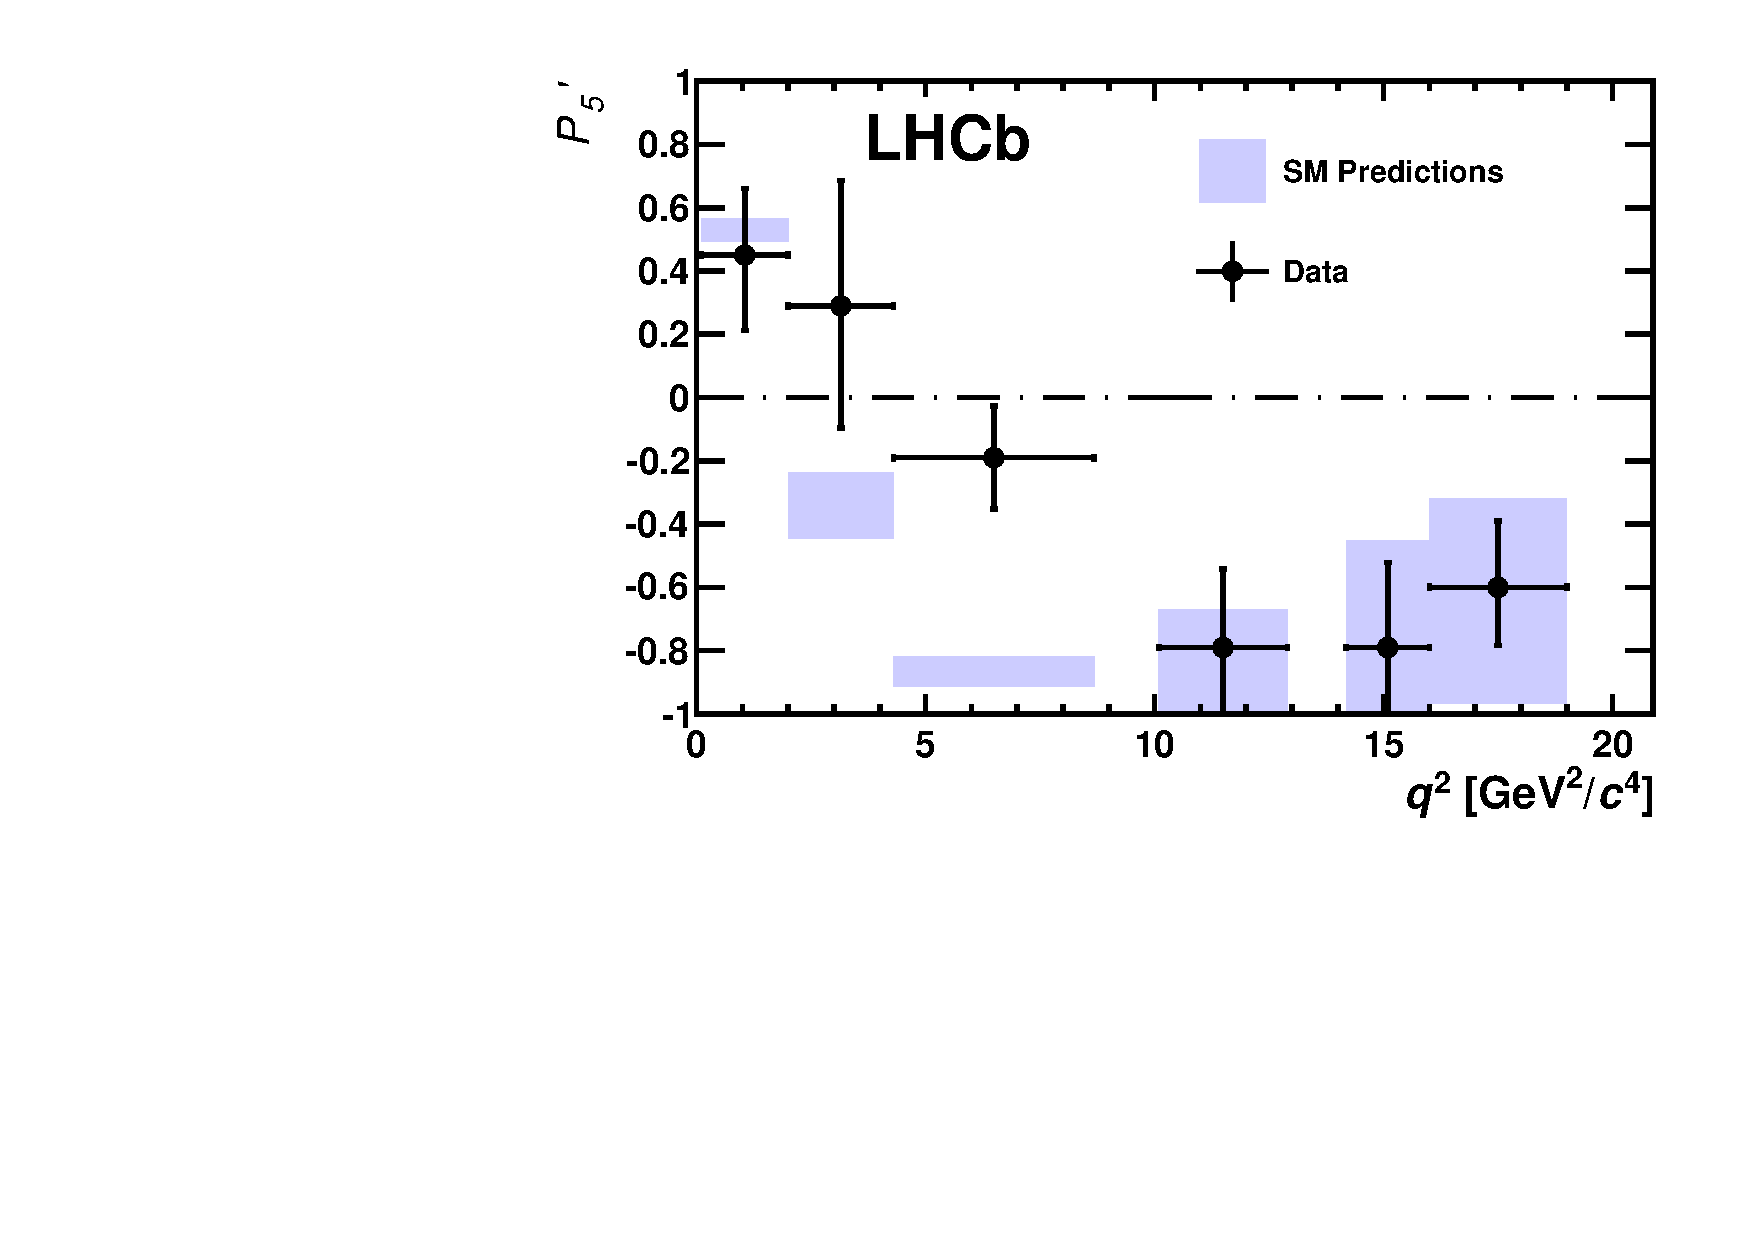
\includegraphics[width=0.6\textwidth]{Introduction/figs/P5prime.pdf}
\caption{Measurement of the $P'_{5}$ observable as a function of \qsq, showing a tension with
SM predictions in the 2--6 \gevgevcccc region~\cite{LHCB-PAPER-2013-037}.}
\label{fig:P5prime}
\end{figure}
%
Other observables for which the sensitivity to form factors effects is reduced are the CP asymmetry between
$B$ and $\bar{B}$ decays, $\mathcal{A}_{CP}$, and the isospin asymmetry between \Bz and \Bu decays, $\mathcal{A}_{CP}$.
Due to the small size of the corresponding CKM elements, CP asymmetries of $\Bz\to K^{(*)}\mumu$
decays are tiny in the SM, $O(10^{-3})$. In BSM models new sources of CP violation can arise and therefore
$\mathcal{A}_{CP}$ measurements are a powerful test of the SM. 
The isospin asymmetry is not zero in the SM due to isospin breaking effects in the form factors.
This is expected to be $\sim1$\% at low \qsq and increase to $\sim10$\% as \qsq tends to zero.
The LHCb experiment, using the full dataset collected in Run I, corresponding to an integrated luminosity of
3~\invfb and $\sim 10^9$ $B$ decays, measured both of these asymmetries to be consistent with
zero~\cite{LHCB-PAPER-2014-006,Aaij:2014bsa}, as reported in Tab.~\ref{tab:AcpAI}. 
%
\begin{table}
\begin{small}
\begin{tabular}{c|cc|cc}
\multirow{2}{*}{}	& \multicolumn{2}{c|}{$\Bz\to K^+\mumu$}			&\multicolumn{2}{c}{$\Bz\to \Kstarz\mumu$}	\\ \cline{2-5}
							& 1.1--6 	[\gevgevcccc]	& 15.0--22.0 [\gevgevcccc] & 	1.1--6 [\gevgevcccc]	& 15.0--19.0 [\gevgevcccc]			\\ \hline
$\mathcal{A}_{CP}$  & $0.004 \pm 0.028$	 				& $-0.005 \pm 0.030$		&	$0.094 \pm 0.047$	& $-0.074 \pm 0.044$ 	\\
$\mathcal{A}_{I}$	& $-0.10^{+0.08}_{-0.09} \pm 0.02$	& $-0.09 \pm 0.08 \pm 0.02$	&	$0.00^{+0.12}_{-0.10} \pm 0.02$  &	$0.06^{+0.10}_{-0.09} \pm 0.02$ \\
\end{tabular}
\end{small}
\caption{Measurement of CP and isospin asymmetry in $\Bz\to \Kstarz\mumu$ decays from the LHCb experiment~\cite{TomRDreview}.  }
\label{tab:AcpAI}
\end{table}
%
Recently, progress was also made measuring electron channels.
The branching fraction of the $\Bz\to\Kstarz\ee$ decay was measured to be $(3.1\pm1.3)\times10^{-7}$ in the dilepton mass interval 30--1000~\mevcc~\cite{LHCB-PAPER-2013-005}. Furthermore, for the first time
angular observables were measured for this decay and found to be consistent with SM predictions~\cite{Aaij:1981106}.

Given the wide set of available measurements, theorists have implemented global fits including results from rare decays analyses,
 as well as inputs from \Bs mixing and Higgs measurements, in order to understand if the existing anomalies could be caused by a common factor.
The results of such global fits agree that there is a tension with respect to the SM at the level of 3--4 standard deviations,
depending on the set of assumptions made. In particular they favour a shift $C^{NP} \sim -1$ to the $C_9$ Wilson
Coefficient, related with the penguin diagram mediated by a $Z^0$ boson~\cite{Altmannshofer:2014rta,Descotes-Genon:2013wba,Hurth:2016fbr}. 

\subsection{Lepton Flavour Violation searches}

Several Lepton Flavour Violation (LFV) searches are linked to rare decays as they involve small branching
ratios in the SM that can be enhanced by BSM physics. %They are therefore a natural place to look for new physics.
Lepton flavour conservation is experimentally well-established measuring the branching ratios of
decays of muons into electrons and no neutrinos, but has no strong theoretical
explanation in the context of the SM. In fact it is already observed that flavour
is not conserved in neutrino oscillations. 
%This section reports a short review of LFV searches. 
%
The best-studied decays violating lepton flavour 
are rare muon decays including $\mu^+\to e^+\gamma$ and $\mu^+\to e^+e^-e^+$.
Since muons can be abundantly produced and the final states are simple,
these decays provide the best constraints to LFV. The current best upper limits are $1.2 \times 10^{-11}$
for the radiative decay and $1.0 \times 10^{-12}$ for \mbox{$\mu^+\to e^+e^-e^+$} obtained
respectively by the MEGA~\cite{Ahmed:2001eh} and SINDRUM~\cite{Bellgardt:1987du} experiments.
Several LFV searches in the $B$ sector have recently been performed at the LHCb experiment 
including decays such as $\Bz\to e\mu$~\cite{LHCB-PAPER-2013-030} and $\tau$ decays such
as $\tau\to\mumu\mu$~\cite{LHCB-PAPER-2013-014}. None of these searches has found evidence 
of new physics so far and therefore they set limits, constraining the parameter space available for BSM models.
Figure~\ref{fig:LFV_decay} shows a summary of the best limits set at different times
on LFV searches~\cite{Marciano:2008zz}.


\begin{figure}[h!]
\centering 
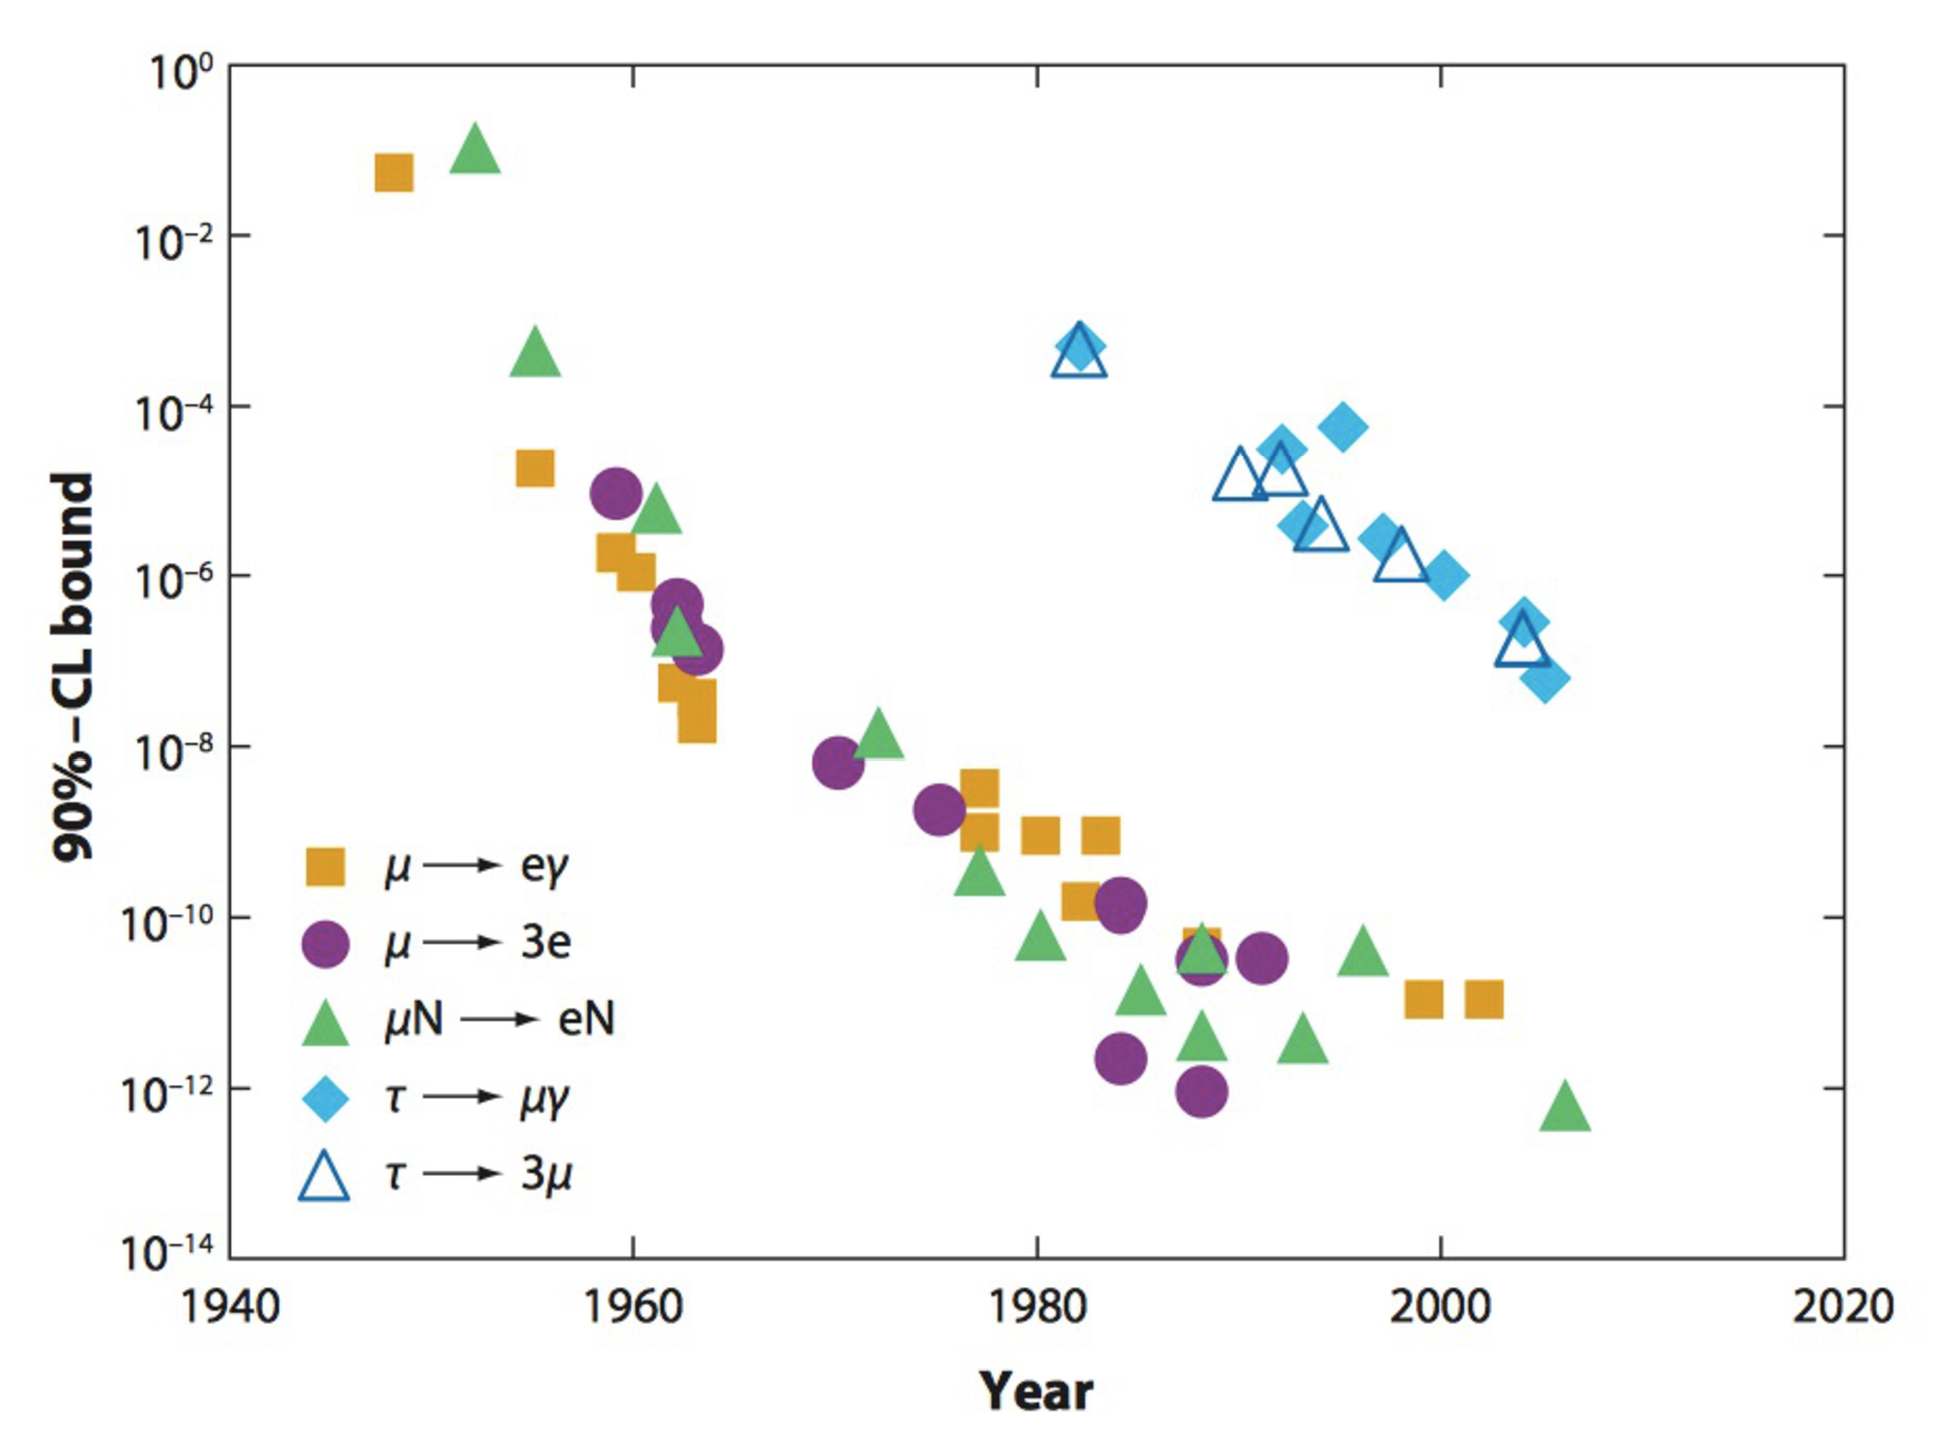
\includegraphics[width=0.7\textwidth]{Introduction/figs/LFV.pdf}
\caption{Summary of limits set in LFV searches as a function of time~\cite{Marciano:2008zz}.}
\label{fig:LFV_decay}
\end{figure}
 

\chapter{The LHCb detector at the Large Hadron Collider}
\label{sec:Detector}

\section{The Large Hadron Collider}

The Large Hadron Collider (LHC) is a circular particle accelerator with a circumference of 27 km about 100 m underground.
The two general-purpose detectors, ATLAS and CMS, sit on opposites sides of the ring, while the two smaller specialty detectors, 
ALICE and LHCb, are at the interaction points to either side of ATLAS (see fig. \ref{lhc}).

\begin{figure}[h!]
\centering
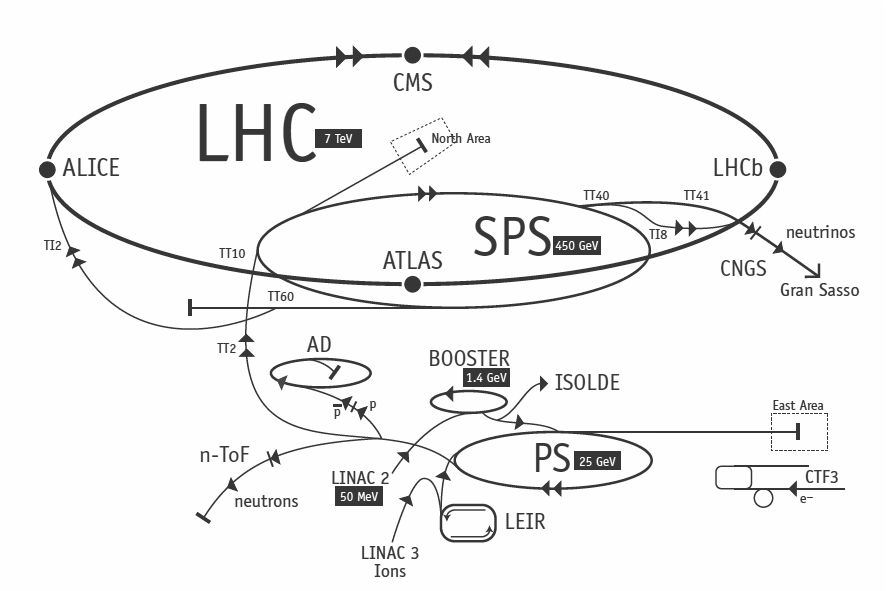
\includegraphics[width=1\textwidth]{Detector/figs/LHC_scheme.png}
\caption{Scheme of CERN accelerators.} \label{lhc}
\end{figure}

Two proton beams circulate in opposite directions around the ring and cross each other at several points, 
in which are placed huge particle detectors. Each beam consists of a series of proton bunches, up to a maximum of 2835
in the beam. Each bunch consists of about $10^{11}$ protons and the bunch spacing is such that the nominal bunch crossing
rate is 40 MHz. The beams are injected into pre-accelerators and then led into LHC through the CERN acceleration
system shown in figure \ref{lhc}. Protons are produced from duoplasmatron, starting from hydrogen gas, and are
initially accelerated to the energy of 50 MeV in a linear accelerator (LINAC). Then, protons are injected into
the Proton Synchrotron Booster (PSB) where they are boosted to an energy of 1.4 \gev, then into the Proton Synchrotron (PS)
to 25 GeV and Super Proton Synchrotron (SPS) to 450 GeV. Finally, protons enter into the LHC storage ring.
In the main ring proton beams are accelerated from injection energy to the final one by radio frequency (RF) cavities.
The beams are steered around the ring by 8 T magnetic fields produced in 15 meter long superconducting niobium-titanium
dipole magnets, and focused by quadrupole and multipole magnets. The LHC magnets use a design in which both proton beam
pipes are contained in the same housing, allowing the same liquid helium to cool the system down for both \cite{lhc}.
The LHC began colliding proton beams in physics mode in 2009 at and energy of $\sqrt{s} = 900$ GeV and from April 2010
to November 2011 accelerated beams at $\sqrt{s} = 7$ TeV (3.5 TeV per proton beam). At this energy it delivered over
$5.7 \text{ fb}^{-1}$ of collisions, with a maximum instantaneous luminosity of $3\cdot10^{33} \text{ cm}^{-2}\text{s}^{-1}$.
The LHC maximum design energy is 14 TeV, and its design luminosity is $10^{34} \text{ cm}^{-2}\text{s}^{-1}$.
After a long shut down to upgrade and maintain the machine, a new run started in June 2015 where protons
are collided at an energy of $\sqrt{s} = 13$ \tev at this energy the total proton-proton cross section
is expected to be roughly 100 mb.
%, thus at the design luminosity the general purpose detectors will an event rate approximately $10^9$ inelastic events/s.

\section{The LHCb detector}

The LHCb detector was built with the main purpose of studying the decays of B and D mesons, looking in particular for CP-violating processes. In 2011, running at a centre of mass energy of 7 TeV, the cross section of $b\bar{b}$ production was measured to be $284 \pm 53 ~\mu b$\cite{Aaij:2010gn}, while it will be $\sim500 ~\mu b$ at the nominal LHC energy, 14 TeV.
At these high energies, proton-proton interactions produce highly boosted virtual gluons which interact to produce $b\bar{b}$ pairs at small angles, close to the beam pipe. For this reason the LHCb detector is designed to have a very forward angular coverage: it is fully instrumented from approximately 10 mrad to 300 mrad, corresponding to $2 < \eta < 5$, where $\eta$ is a quantity used in particle physics and called ``pseudorapidity" and defined as:
\begin{equation}
\label{pseudorap}
\eta = - \ln(\tan(\theta/2))
\end{equation}
In Eq. \ref{pseudorap}, $\theta$ is the angle between a particle's momentum and the beam direction\footnote{LHCb's reference system has the $z$ axis in the direction of the beam, the $x$ axis directed to the centre of the accelerator and $y$ is directed upward. Then we define $\theta$ as the angle with the beam direction and $\phi$ as the position around the beam in the $xy$ plane, taking $\phi = 0$ on the $x$ axis.}.

\begin{figure}[h]
\label{lhcb}
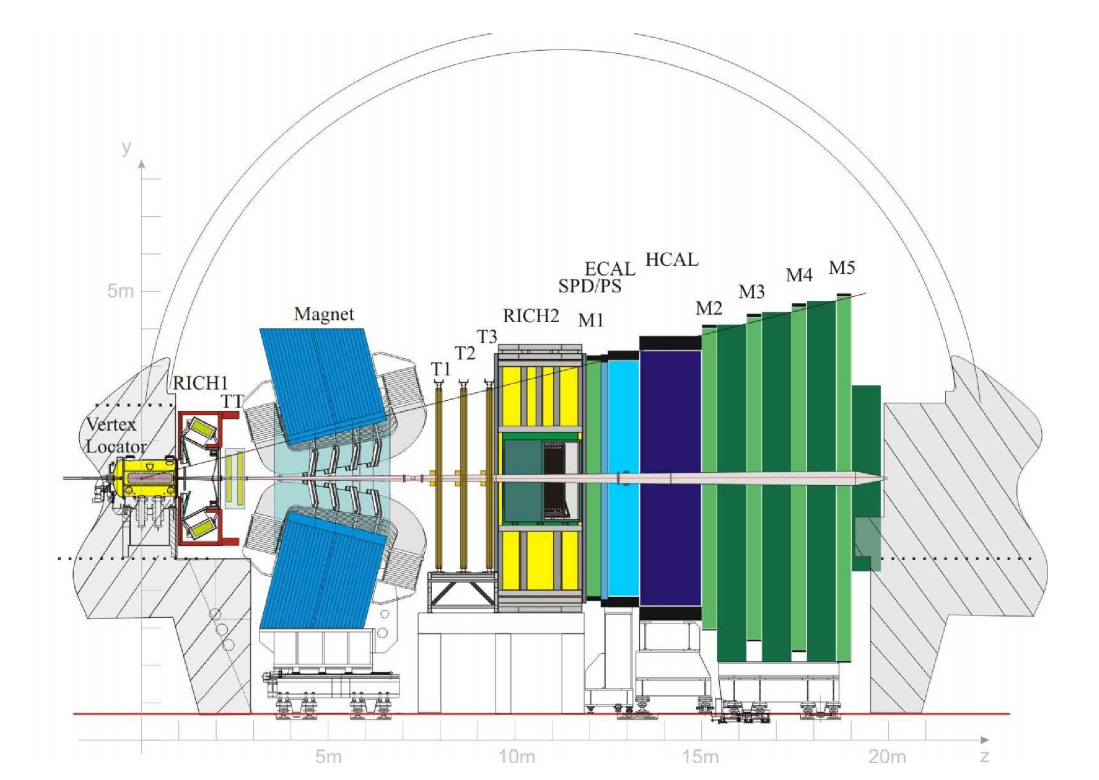
\includegraphics[width=0.9\linewidth]{Detector/figs/LHCb_official.png}
\caption{A side view of the LHCb detector \cite{Alves:2008zz}.}
\end{figure}

At the collision point of LHCb the luminosity can be adjusted by displacing the beams from head on collisions while keeping the same
crossing angle. This allows the experiment to keep an approximately constant instantaneous luminosity. This also means that the average number of interactions per bunch crossing can be limited as LHCb efficiency, especially of detecting secondary vertices, decreases for events with an high number of primary vertices (PV). Reducing the particle occupancy through the detector also keeps radiation damage to a minimum. Since the LHC started colliding protons in
November 2009 until the end of 2011, the instantaneous luminosity was at an average of $3 \cdot 10^{32} \mbox{cm}^{-2}\mbox{s}^{-1}$, with an average number of 1.5 vertices per bunch crossing in LHCb. At the end of 2011 LHCb had collected an integrated luminosity of $1 ~\mbox{fb}^{-1}$; in 2012 the luminosity was increased and $2 ~\mbox{fb}^{-1}$ more were collected.

Other B physics experiments, like BaBar at the Stanford Linear Accelerator (SLAC), Belle at KEK at J-PARC (Japan) and the Tevatron experiments at Fermilab have made accurate measurements in heavy flavour physics. All of these results have so far been consistent with the Standard Model predictions. However, some of the deviations from the Standard Model are expected to be very small, therefore LHCb has begun to make the most precise measurements in heavy flavour physics.

The LHCb detector\cite{Alves:2008zz} includes a high-precision tracking system consisting of a silicon-strip vertex detector surrounding the $pp$ interaction region, a large-area silicon-strip detector located upstream of a dipole magnet with a bending power of about 4 Tm, and three stations of silicon-strip detectors and straw drift tubes placed downstream. The combined tracking system has momentum resolution $\Delta p/p$, that varies from 0.4\% at 5 $\mbox{GeV/c}^{2}$ to 0.6\% at 100 $\mbox{GeV/c}^{2}$.
Charged hadrons are identified using two Ring-Imaging Cherenkov detectors (RICH)\cite{LHCb-DP-2012-003}. Photon, electron and hadron candidates are identified by a calorimeter system consisting of scintillating-pad and pre-shower detectors, an electromagnetic calorimeter and a hadronic calorimeter. Muons are identified by a system composed of alternating layers of iron and multiwire proportional chambers\cite{LHCb-DP-2012-002}. A schematic view of the detector is shown in Fig. \ref{lhcb}.


\subsection{Tracking system}

The tracking system is made up of the Vertex Locator (VeLo), and 4 tracking stations: the Tracker Turicensis (TT) which are located before the magnet and T1, T2 and T3 which are downstream of the magnet. Charged particle tracks are bent horizontally in the magnetic field so that their momentum can be measured from the curvature radius.

B mesons have lifetimes of approximately 1.5 ps. At the LHC energies, this means they travel about 1 cm before decaying and they form a displaced vertex. It is therefore important to be able to separate the particles produced at the primary $p-p$ vertex and the B decay vertex.

The VeLo accurately measures positions of tracks close to the interaction point so that production and decay vertices of bottom and charm hadrons can be reconstructed. The VeLo is made up of 21 staggered silicon modules which surround the beam axis and are positioned from $z = -18$ cm to $+80$ cm. It is able to detect particles within a pseudorapidity range $1.6 < \eta < 4.9$. The sensitive region of the VeLo starts at an inner diameter of 8mm from the beam axis. The VeLo is housed in its own vacuum vessel of thin aluminium foil which protects the vacuum of the beam pipe from any outgassing of the VeLo. VeLo stations consist of two modules, and each has two types of sensors: the $\phi$-sensor which measures the azimuthal position around the beam, and the R-sensor which measures the radial distance from the beam axis. A sketch of the VeLo sensor is shown in Fig. \ref{VeLo}. The sensors are 300 $\mu m$ thick, approximately semicircular and are positioned on either side of the beam axis. To ensure that they cover the full azimuthal angle the right-side module is placed 1.5 cm behind the left-side module on the z-axis and they overlap. There are two modules which cover the backward direction and were used as a veto for multiple interactions in 2011, called the pileup veto.

\begin{center}
\begin{figure}[h!]
\label{VeLo}

\begin{minipage}{0.49\textwidth}

\centering 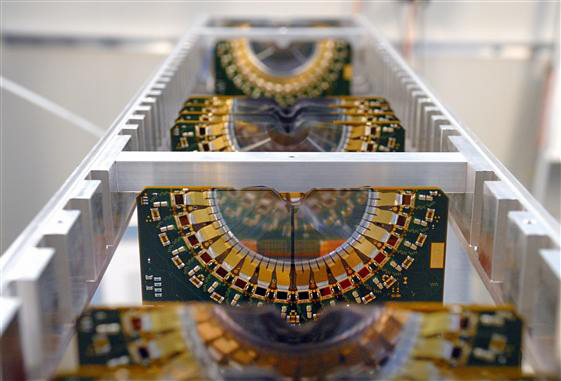
\includegraphics[width=0.8\textwidth]{Detector/figs/detector/VELO.png}

\end{minipage}
\begin{minipage}{0.49\textwidth}

\centering 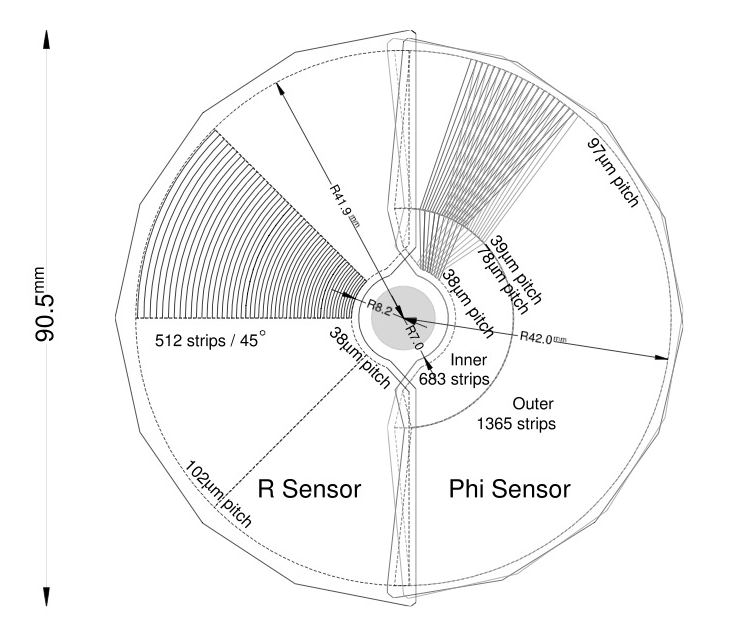
\includegraphics[width=0.8\textwidth]{Detector/figs/detector/VELO_scheme.png}

\end{minipage}
\caption{On the left VeLo sensors mounted in line and on the right a schematic view of one sensor \cite{Alves:2008zz}.}
\end{figure}
\end{center}

The LHCb dipole magnet is comprised of two coils supported on an iron yoke and is wedge-shaped to fit the LHCb 
angular acceptance. It is a warm magnet so can be ramped easily and the field can be reversed periodically. 
This is used to limit some systematics that can arise form imperfections performance in different areas of the detector.

The IT and TT both use silicon microstrip and together constitute the Silicon Tracker (ST). Straw tubes are used 
in the outer regions of the tracking stations which together are called the Outer Tracker (OT). The IT has 
an higher inner granularity because of the higher flux of particles nearer the beam pipe. Each ST station 
has four detection layers, the first and last being vertical, measuring the track position in x. The second 
and third layer are rotated by a stereo angle of +5 and -5 degrees, which allows the y-coordinate to be measured. 
The TT is placed upstream of the magnet which allows reconstruction of the tracks from low-momentum particles which 
are swept out of the downstream acceptance.

\subsection{Particle identification}

Particle identification in LHCb is performed in various ways. The calorimeter detects particles with high 
transverse momentum, the muon chambers identify muons and the Ring Imaging Cherenkov (RICH) detectors identify 
heavier charged particles.

\subsubsection{Calorimeters}
\label{sec:calorimeters}

The main purpose of the calorimeter system is to determine the energy of particles traversing the detector. 
The material in the calorimeter system is layered with absorber and active material. The absorber makes particles
interact and produces a cascade of secondaries, which multiply quickly and are detected by the active part. 
The sensitive material consists of scintillating layers, where the light detected is approximately proportional 
to the number of deposited particles. Calibration is then used to calculate the deposited energy. The calorimeter 
system is essential for flavour tagging because it identifies electrons. In addition, it is required for accurately 
reconstructing
$\pi^0$ particles and prompt photons, which are both needed for the study of B-meson decays. The LHCb calorimeter 
system consists of the Scintillator Pad Detector (SPD), the Pre-Shower Detector (PS) as well as the Electromagnetic 
Calorimeter (ECAL) and the Hadronic Calorimeter (HCAL). All four detectors transmit scintillation light via 
wavelength-shifting fibres to photo-multiplier tubes (PMTs). The SPD/PS cells are read out with MAPMTs 
(Multi-anode PMTs) located outside the LHCb acceptance. The ECAL and HCAL have individual MAPMTs located on the modules.
All four detectors vary the segmentation of their cells according to the distance from the beam pipe.
The purpose of the SPD and PS is to separate the electrons from a high background of neutral and charged pions 
produced in the collisions. In order to obtain the highest energy resolution the showers from high energy photons 
must be fully absorbed. For this reason the ECAL has a thickness of 25 radiation lengths and its resolution is 
measured to be \cite{Alves:2008zz}
 
 \begin{equation}
 \frac{\sigma_{ECAL}(E)}{E} = \frac{10\%}{\sqrt{E(GeV)}} + 1\%
 \end{equation}

The trigger requirements on the HCAL resolution do not depend on the containment of the hadron showers as much 
as for the ECAL, so due to a limited space, its thickness is only 5.6 interaction lengths and its resolution

 \begin{equation}
 \frac{\sigma_{HCAL}(E)}{E} = \frac{69\%}{\sqrt{E(GeV)}} + 9\%
 \end{equation}




\subsubsection{RICH}

The two RICH detectors are a special feature of LHCb, as it is the only experiment at LHC including them. 
These detectors take advantage of the  Cherenkov light produced by particles passing in a medium with velocity 
higher that the velocity of light in the medium. The Cherenkov light, as shown in Fig. \ref{Cherenkov}, 
is produced in cones with a specific angle depending on the velocity of the particle

\begin{equation}
cos(\theta) = \frac{1}{\beta n}
\end{equation}

where $\beta$ is the velocity of the particle over $c$ and $n$ is the refraction index of the medium.

\begin{center}
\begin{figure}[h!]
\label{Cherenkov}

\begin{minipage}{0.45\textwidth}

\centering 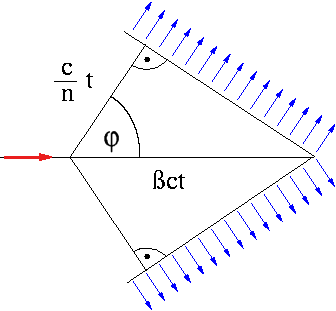
\includegraphics[width=0.8\textwidth]{Detector/figs/detector/Cherenkov.png}

\end{minipage}
\begin{minipage}{0.55\textwidth}

\centering 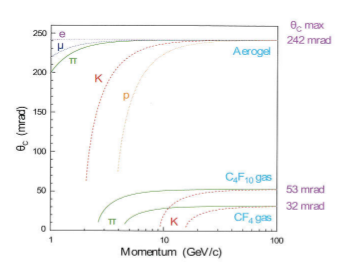
\includegraphics[width=0.8\textwidth]{Detector/figs/detector/RICH_performance.png}

\end{minipage}
\caption{On the left a sketch of Cherenkov light emission \cite{wikiCherenkov} and on the right the Cherenkov
angle versus momentum for the two radiators of RICH1 and for different particles. One can see that they allow
to separate particles in different momentum ranges.}
\end{figure}
\end{center}

RICH 1 is situated before the magnet in order to cover a large angular acceptance. Its purpose is to ensure
particle identification over the momentum range $1 < p < 70$ GeV. It uses two radiators, $C_4F_{10}$ covers
the momentum range $5 - 70$ GeV/c, and silica aerogel which covers $1 - 10$ GeV/c. RICH 2 is situated after
the magnet and tracking stations. It identifies higher momentum particles from approximately 20 GeV up to beyond
100 GeV using $CF_4$ as a radiator.
The Cherenkov light produced when charged particles travel through the radiators, is reflected and focused using
flat and spherical mirrors which are tilted so that the ring image is reflected onto arrays of photo-detectors.
The radius of the ring becomes equivalent to the opening angle of the Cherenkov cone because of the known geometry.
The photo-detectors are located outside of the LHCb acceptance in order to reduce the amount of material that
the particles have to traverse. Pattern recognition algorithms are then used to reconstruct the Cherenkov rings.

For particle identification a particle type hypothesis is assigned to each charged track found in the tracking stations.
Initially the hypothesis is for a pion, which is the most common particle type. The corresponding expected number and
Cherenkov radii of the resulting photons are calculated and the likelihood is calculated. The hypothesis is then changed
and the likelihood is recalculated. The case with the largest increase in likelihood is kept.


\subsection{The muon system}

\begin{figure}[b!]
\label{muonsystem}
\centering 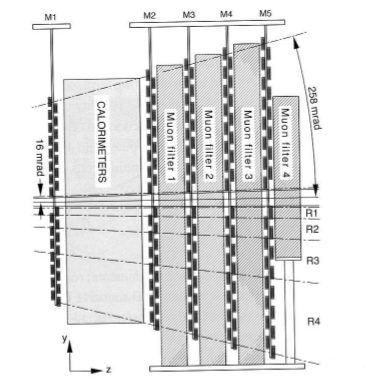
\includegraphics[width=0.5\linewidth]{Detector/figs/muonsystem.png}
\caption{The LHCb muon system \cite{Alves:2008zz}.}
\end{figure}

It is essential for many of the key physics analyses to be able to identify muons in the final state.
Muons are the most penetrating particles that can be detected at LHC experiments, so the muon chambers
are the final subdetectors. There are five stations (M1 - M5), the first one being located before the calorimeter
in order to improve the $p_T$ measurements. A scheme of the muon system is shown in Fig. \ref{muonsystem}.

The remaining four lay behind the HCAL and are separated by 1.2 m from each other, interleaved with iron block
filters 80cm thick, which absorb hadrons, electrons and photons to ensure that only muons reach the final muon station.
Only muons with a minimum momentum of 10 GeV/c traverse all of the five stations and for positive identification of a muon
the trigger requires a signal in each of them. Each station has a detection efficiency of at least 95\% and the detectors
provide position measurements. Since there is a larger particle flux towards the beam pipe, the stations are divided
into four concentric rectangular regions (R1-R4), their size increasing according to the ratio 1 : 2 : 4 : 8.
This means that there is a similar channel occupancy over the four regions. All of the muon stations use
Multi Wire Proportional Chambers (MWPC) except for the inner region of M1, where the particle flux is too high.
In this region triple-GEM (Gas Electron Multiplier) detectors are used instead because they have better ageing properties.

The Gas Electron Multiplier (GEM) detectors in the inner region of M1 have to  withstand a rate up to
$500 ~\mbox{kHz cm}^{-2}$ of charged particles. Particles traversing through the drift gap between the cathode
and the first GEM foil produce ionisation electrons which are then attracted by electric fields though all of the
GEM foils and they multiply. They then drift into the anode inducing a signal on the pads. A gas mixture of Argon,
$CO_2$ and $CF_4$, is used to give a time resolution better than 3 ns.




\subsection{Trigger and software}

The LHCb trigger system\cite{LHCb-DP-2012-004} consists of a hardware stage (L0), based on information from the calorimeter
and muon systems, followed by a software stage (HLT), which applies a full event reconstruction. To increase performances
the HLT is split again into stages (HLT1 and HLT2). The bunch crossing frequency is $40 ~\mbox{MHz}$, which corresponds
to an instantaneous luminosity of $2 \cdot 10^{32} ~\mbox{cm}^{-2} \mbox{s}^{-1}$ for LHCb, and about 15\% of the total
number of $b\bar{b}$ pairs produced will have at least one B meson with all of its decay products within the detector acceptance.
This needs to be reduced down to about 2 kHz so that the events can be written to disk for analysis. Fig. \ref{triggerscheme}
shows a scheme of the trigger system.

The L0 reduces the rate of visible interactions from 10 MHz to a rate of 1 MHz and uses mainly the information from the 
calorimeter dividing the events in the 5 categories: L0Photon, L0Electron, L0LocalPion, L0GlobalPion, L0Hadron. ``local" pions
refer to $\pi^0$ reconstructed though decay in $\gamma\gamma$, where the two photons fall in the same ECAL board, they are
labelled ``global" otherwise. The HLT1 uses information from the VELO and trackers performing a partial reconstruction
of the event and reduces the rate to 2 kHz. Finally the HLT2 involves a full reconstruction of the event and includes many
``lines" designed to trigger specific decays.

LHCb also developed an extended simulation software in order to reconstruct efficiencies and signal shapes.
In the simulation, $pp$ collisions are generated using $\textsc{Pythia}$~6.4\cite{Sjostrand:2006za} with a specific
LHCb configuration\cite{LHCb-PROC-2010-056}. Decays of hadronic particles are described by $\textsc{EvtGen}$\cite{Lange:2001uf},
in which final state radiation is generated using $\textsc{Photos}$\cite{Golonka:2005pn}. The interaction of the generated
particles with the detector and its response are implemented using the $\textsc{Geant4}$ toolkit\cite{Allison:2006ve, *Agostinelli:2002hh}
as described in \cite{LHCb-PROC-2011-006}.

For the analysis in this document, I used the ROOT framework\cite{Brun:2000es} to analyse data, the RooFit package
fot fitting. The multivariate analysis is base on ne NeuroBayes package \cite{} which provides a framework
for neural network training.

\begin{figure}[t!]
\label{triggerscheme}
\centering 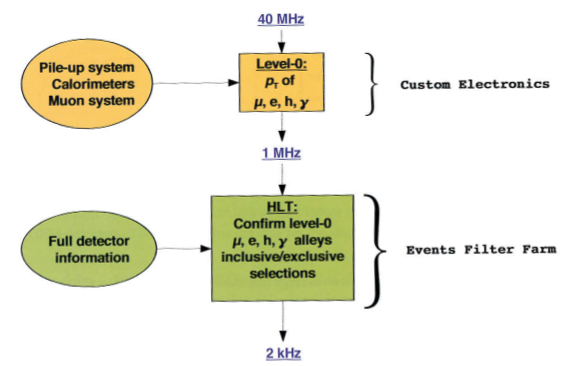
\includegraphics[width=0.8\linewidth]{Detector/figs/triggerscheme.png}
\caption{Scheme of the LHCb trigger system \cite{Alves:2008zz}.}
\end{figure}







\section{Selection}
\label{sec:RKst_selection}

The selection process, described in this section, is divided into several steps:
\begin{itemize}
\item candidates have to fall into the detector acceptance, produce hits and be selected
on the basis of quality variables, such as \chisq of tracks and vertices and basic kinematic cuts.
%This stage is called ``stripping". 
Furthermore, it is required that the events are triggered by specific
trigger lines and cuts are applied to remove backgrounds from specific decays.
All these first three steps are referred to as ``pre-selection";
\item secondly, PID requirements are applied to remove part of misreconstructed
background and clear the way for the last step;
\item in the final step a neural network is used to remove combinatorial background. Furthermore,
for the electron channels, which are more challenging, the kinematic structure of the decays
is also used to improve the purity of the samples.
\end{itemize}
%
%In order to minimise the systematic uncertainties the same selection requirements are used to select 
%the rare signal candidates and the relative charmonium channel, a part from the \qsq cuts which serve
%to distinguish them. 
To identify the $\jpsi(\mu\mu)$ candidates a dimuon invariant mass
interval of 100~\mevcc~around the nominal \jpsi peak~\cite{PDG2014} is selected.
On the other hand, it is not possible to use a narrow interval around $\jpsi(ee)$ mass peak as the invariant mass
distribution is characterised by a long radiative tail at low masses due to bremsstrahlung radiation.
Furthermore, a requirement on $m(ee)$ would distort the 4-body $m(K\pi ee)$ mass distribution. This is not advisable 
as it is important to be able to fit a wide mass range to constrain the backgrounds. For these reasons the interval used to 
select $\jpsi(ee)$ candidates extends as low as possible in \qsq without overlapping with
the rare channel interval. Candidates are therefore identified as $\jpsi(ee)$ if they fall in the \qsq interval
$6 < \qsq < 11$~\gevgevcccc. Similarly, candidates are identified as $\psitwos(ee)$ is they fall into $11 < \qsq < 15$~\gevgevcccc
and $\gamma(ee)$ if they fall into $\qsq < 0.0004$~\gevgevcccc.
Table~\ref{tab:candidates} summarises the requirements used to distinguish samples corresponding to different decay channels.
Figure~\ref{fig:2D_q2_B0mass} shows two-dimensional distributions of \qsq versus the 4-body invariant mass 
for candidates passing the full selection. Horizontal bands can be clearly seen at \qsq values corresponding to the \jpsi and \psitwos resonances.
On the plot for muons a vertical band which corresponds to the rare decay is also evident.

\begin{table}[t!]
\begin{center}
\caption{Summary of the channel categories.}
\label{tab:candidates}
\begin{footnotesize}
\renewcommand\arraystretch{1.4}
\begin{tabular}{$c|^c|^c}
\rowstyle{\bfseries}
 Type & Sample & \boldmath{\qsq} \\
\hline
\multirow{4}{*}{$\mu\mu$}
	& \BdToKstmm (low)			& $0.0004<\qsq<1.1\gevgevcccc$ \\
	& \BdToKstmm (central)		& $1.1<\qsq<6\gevgevcccc$ \\
	& \BdToKstmm (high)		& $\qsq>15\gevgevcccc$ \\
	& \BdToKstJPsmm (\mcKpimm)	& $|m_{\mu\mu} - m_{\jpsi}^{PDG}| < 100\mevcc$ \\ \hline
\multirow{7}{*}{$ee$} 
	&  \BdToKstee (low)			& $0.0004<\qsq<1.1\gevgevcccc$ \\
	& \BdToKstee (central)		& $1.1<\qsq<6\gevgevcccc$ \\
	& \BdToKstee (high)			& $\qsq>15\gevgevcccc$ \\
	& \BdToKstJPsee (\mcKpiee)	& $6<\qsq<11\gevgevcccc$ \\
\cline{2-3}
	& \multicolumn{2}{c}{Control samples} \\ \cline{2-3}
	& \BdToKstGee (\mKpiee)		& $\qsq<0.0004\gevgevcccc$ \\
	& \BdToKstJPsee (\mKpiee)	& $6<\qsq<11\gevgevcccc$ \\
	& \BdToKstPsiee (\mcKpiee)	& $11<\qsq<15\gevgevcccc$ \\
\end{tabular}
\end{footnotesize}
\end{center}
\end{table}

\begin{figure}[t!]
\centering 
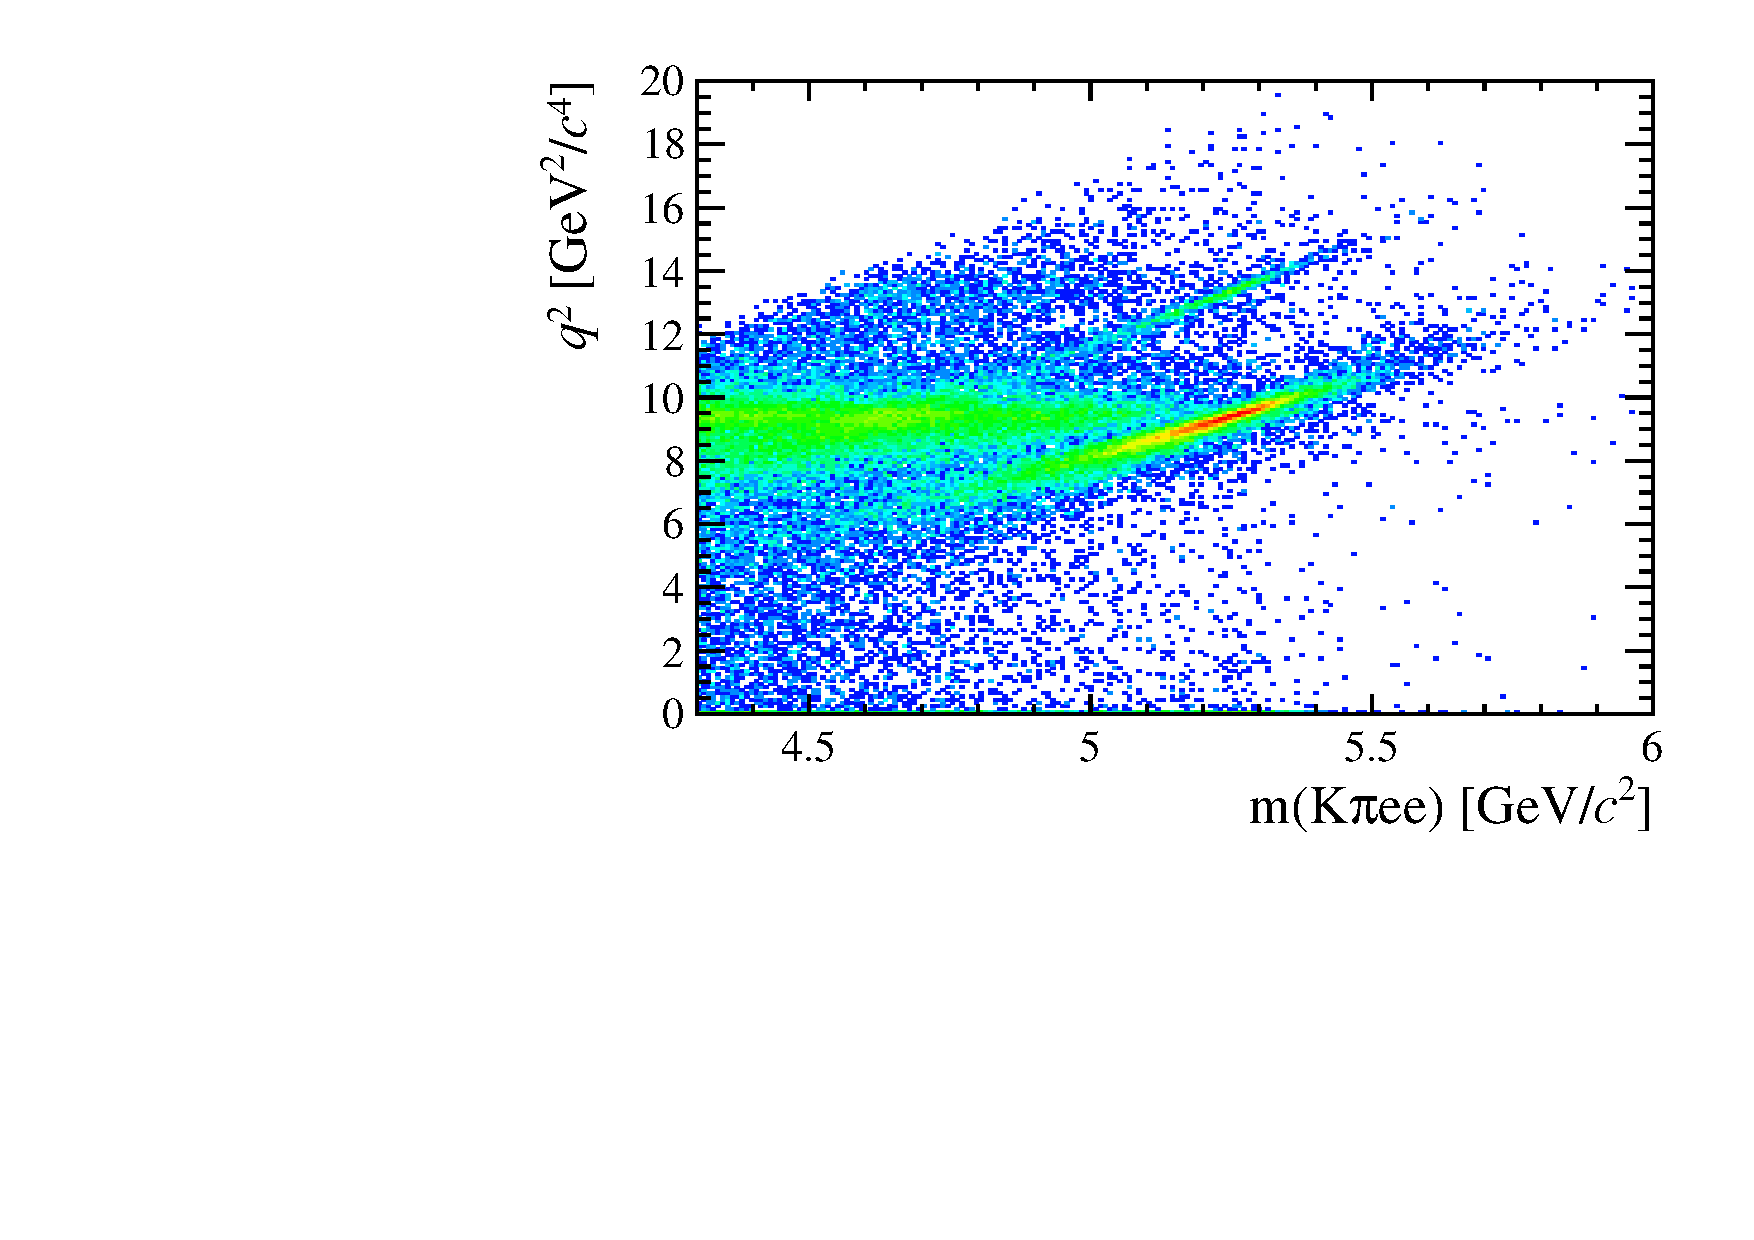
\includegraphics[width=1.\textwidth]{RKst/figs/electron_B0jpsi2D_selected.pdf}
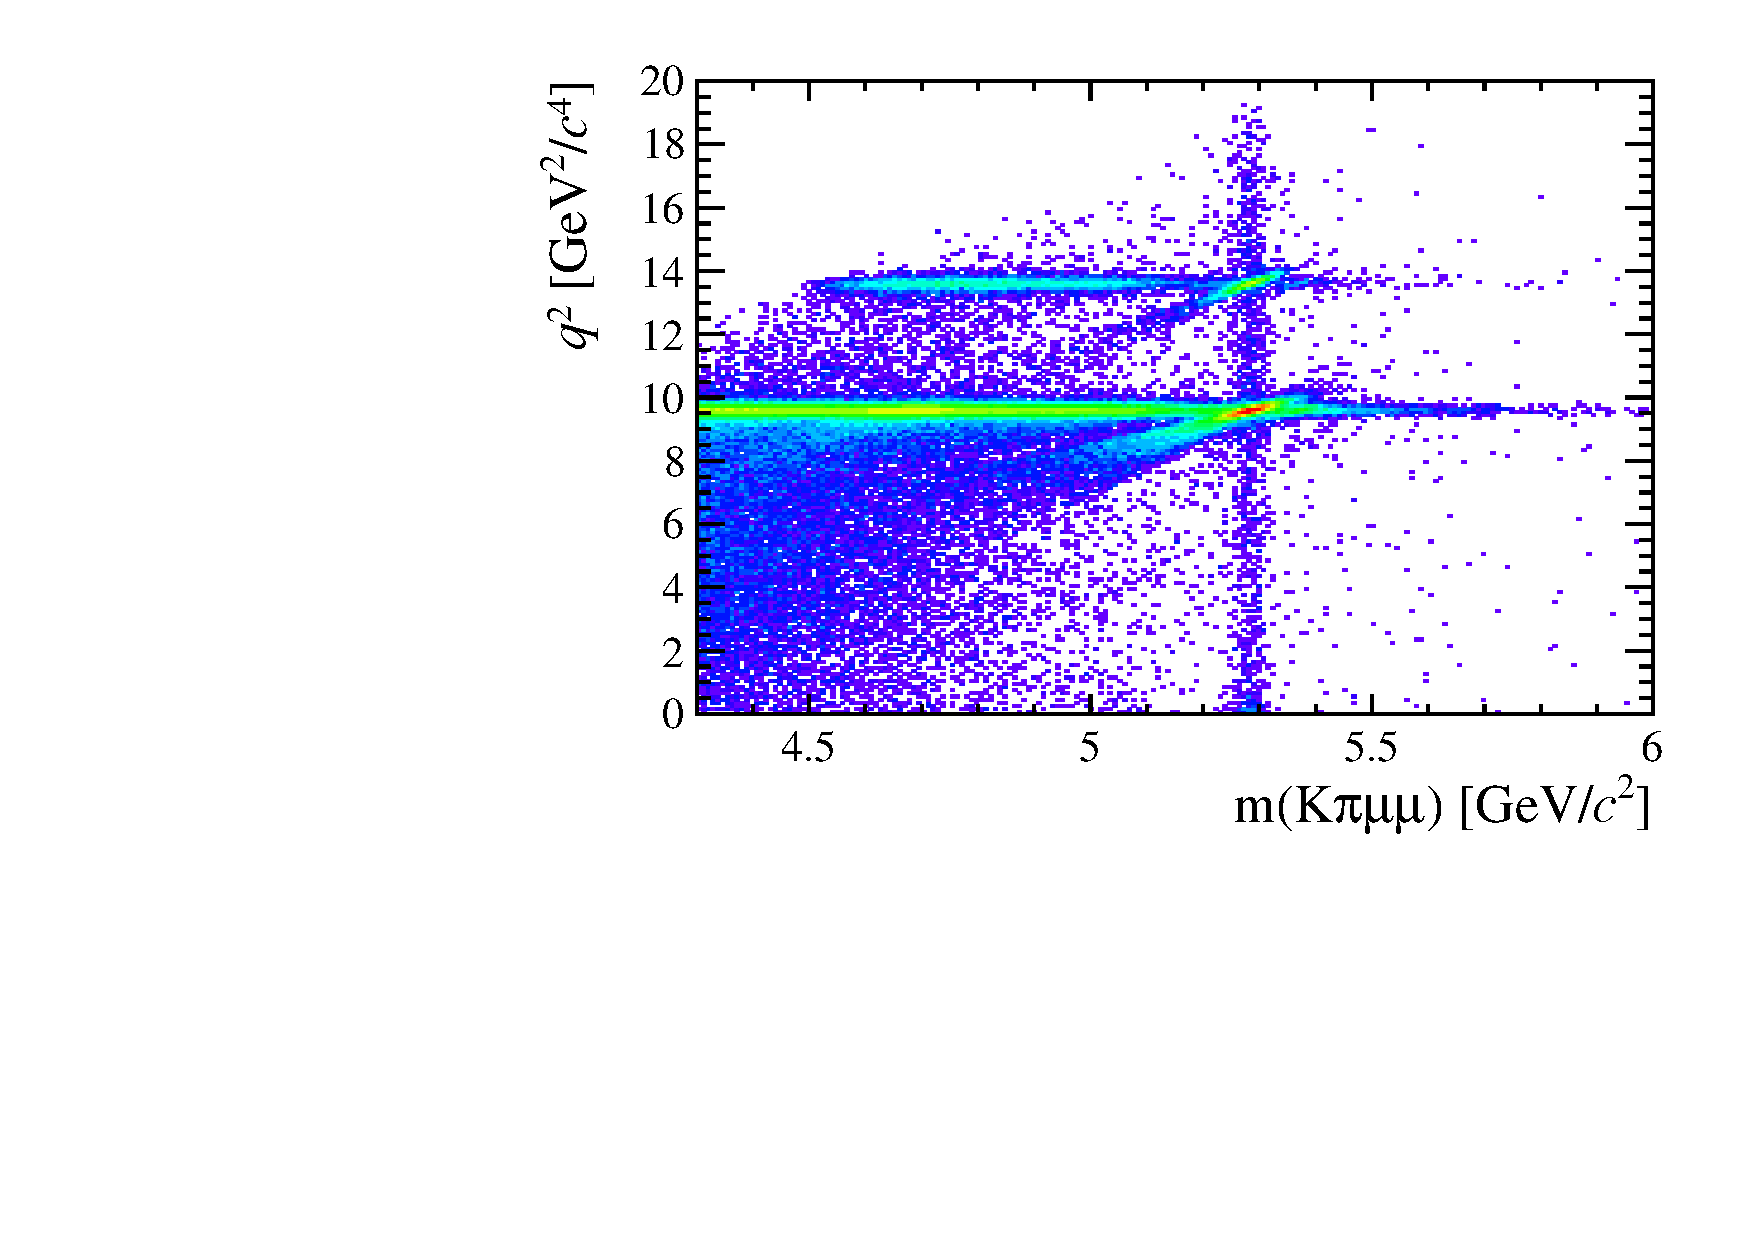
\includegraphics[width=1.\textwidth]{RKst/figs/muon_B0jpsi2D_selected.pdf}
\caption{Two-dimensional distributions of \qsq versus 4-body $m(K\pi\ell\ell)$
invariant mass for the electron (top) and muon (bottom) channels in 2012 data.}
\label{fig:2D_q2_B0mass}
\end{figure}


\subsection{Trigger and pre-selection }
\label{sec:RKst_trigstripping}

Events are triggered for the $\mu\mu$ and the $ee$ channels by the trigger lines
reported in Tab.~\ref{tab:RKst_triglines}, where the logical $and$ of L0, HLT1 and HLT2
lines is required and the logical $or$ of the lines on the same level. The candidates are
required to be triggered-on-signal (TOS) for most of the stages, namely it is required that the 
particle responsible for the trigger decision is one of the particles used to build the signal candidates.
Only for \verb!L0Global!, used in the electron case, a trigger-independent-of-signal (TIS) is required. 
%this is aimed to collect all the possible statistics for the electron channels, which are the most challenging.
The \verb!L0Muon! trigger requires hits in the muon detector, while \verb!L0Electron! and \verb!L0Hadron! use information
from the calorimeters; \verb!HLT1TrackAllL0! adds information from the trackers and
triggers if the L0 decision is confirmed; finally, \verb!HLT2Topo[2,3]BodyBBDT! uses a full reconstruction 
of the event and a neural network trained on candidates with a specific topology in order to detect specific decay structures.
%More information about the muon triggers can be found at Sec.~\ref{sec:Lb_trigger}.

\begin{table}[h!]
\begin{center}
\caption{Summary of the trigger lines used to select the $\mu\mu$ and the $ee$ channels.
Where not explicitly indicated, the lines are required to be TOS.}
\begin{tabular}{$c|^c|^c}
\rowstyle{\bfseries}
Trigger level & \boldmath{$\mu\mu$} candidates &  \boldmath{$ee$} candidates \\
\hline
\multirow{3}{*}{L0}     & 	\multirow{3}{*}{L0Muon}		&    	L0Electron	\\
				&							& 	L0Hadron\\
				&							& 	L0Global (TIS)\\
\hline
\multirow{2}{*}{HLT1}		&	Hlt1TrackAllL0				& \multirow{2}{*}{Hlt1TrackAllL0} \\
					&	Hlt1TrackMuon				&	 \\
\hline
\multirow{3}{*}{HLT2}		&	Hlt2Topo[2,4]BodyBBDT 		& Hlt2Topo[2,4]BodyBBDT \\
					& 	Hlt2TopoMu[2,4]BodyBBDT 	& Hlt2TopoE[2,4]BodyBBDT \\
					& 	Hlt2DiMuonDetachedDecision	&							\\
\end{tabular}
\label{tab:RKst_triglines}
\end{center}
\end{table}

For the electron channels the L0 lines have different properties, therefore the analysis 
is performed separately for three categories of events, depending on the L0 trigger that fired 
them. These categories are defined to be exclusive in the following way:
%
\begin{itemize}
\item {\bf L0E}: events triggered by at least one of the electrons in the signal candidate (\verb!L0Electron_TOS!);
\item {\bf L0H}: events triggered by at least one of the hadrons in the signal candidate and not in the L0E category \\
 (\verb|L0Hadron_TOS && !L0Electron_TOS|);
\item {\bf L0I}: events triggered by particles independent of any signal candidate and not included in the previous categories\\
(\verb|L0Global_TIS && !(L0Electron_TOS |\verb!|| L0Hadron_TOS)!).
\end{itemize}

The majority of the selected events falls into the L0E category, while
the L0H category is more efficient at low \qsq were the \Kstarz has higher momentum.
Because L0I is defined to be independent of the signal candidate, the corresponding
signal efficiency is the same in both the rare and resonant cases and therefore cancels in their ratio.

Candidates are then required to pass the kinematic and quality cuts summarised in Tab.~\ref{tab:RKstripping},
where the meaning of the variables was already explained in Sec.~\ref{sec:Lb_selection}.
Loose PID requirements are applied in pre-selection to limit the size of the samples, while tighter cuts 
are applied in a second stage. A wide mass window is kept around the \Bz peak so that
 the sideband can be used to train the multivariate classifier and to constrain the backgrounds.
%
%In the table $IP_{\chi_2}$ is defined as the projected distance from the vertex divided by its uncertainty, for example $IP^B_{\chi_2}(primary) > 4$ means
%that the B vertex is 2 standard deviations away from the primary vertex.
%Another quantity used is a pointing variable defined as the angle between the direction of the particle momentum and the flight direction from its mother vertex, called DIRA.
%This allows the selection of particles with well-defined primary vertices.
%%$GhostProb$ is the probability, estimated from the reconstruction algorithm, for the track to be a ghost. 
%Loose PID cuts are applied in preselection to limit the size of the samples, while tighter cuts are applied
%in a second stage. To quantify the PID of a particle the pion is used as a reference point and a Log-Likelihood
%variable is used. Therefore the {\verb PID } variable reported in the table is given in terms of the difference between
%the Log-Likelihood of the particle of a given type and a pion. This is called Delta Log-Likelihood (DLL).
%For example:
%\begin{equation}
%\verb!PID!_K = \text{DLL}_{K-\pi} = \log(\mathcal{L}_K) - \log(\mathcal{L}_\pi)
%\end{equation}
%
\begin{table}[]
\begin{center}
\caption{Summary of pre-selection requirements. Variables are defined in Sec.~\ref{sec:Lb_selection}. }
\begin{tabular}{$c^c}
\rowstyle{\bfseries}
Particle &  Requirements \\
\hline
%\multirow{2}{*}{ All final}
%       			&   track $\chi_2/\text{ndf} < 3$ \\
%       			&   {\verb GhostProb } $< 0.4$ \\
%\hline
$\pi$			& $\chisqip(primary) > 9$ \\      			
\hline
\multirow{3}{*}{K}
      			& {\verb PID }$_K > -5$ \\
       			& $\chisqip(primary) > 9$ \\
       			& {\verb hasRICH }  \\
 \hline
\multirow{4}{*}{ \Kstarz }
       			& $\pt > 500$ \mevc \\
       			& $|m_{K\pi} - m_{\Kstarz}^{PDG}| < 300$ \mevcc  \\ %300 in stripping but then we restrict it to 100
       			& $\chisqip(primary) > 9$ \\
       			& Origin vertex $\chisq/\text{ndf} < 25$ \\
\hline
\multirow{3}{*}{ $\mu$ }
       			& $\pt > 300$ \mevc \\
       			& $\chisqip(primary) > 9$ \\
       			& i{\verb sMuon }\\  %RequiresDet='MUON'
%       		& hasMuon \\
\hline
\multirow{4}{*}{ $e$ }
       			& $\pt > 300$ \mevc \\
       			& $\chisqip(primary) > 9$ \\
       			& {\verb hasCalo }\\ %RequiresDet='CALO'
       			& \verb!PID!$_e > 0$ \\
\hline
\multirow{4}{*}{ $\ell\ell$ }
				& $m_{\ell\ell} < 5500$ \mevcc \\
			  	& End vertex $\chisq/\text{ndf} < 9$ \\
			  	& Origin vertex $\chi^2$ separation $> 16$ \\
%			  	& $\chisqip(primary) > 0$ \\
\hline
\multirow{4}{*}{ $B^0$  }
 %      & $| m - m_{B^0}^{PDG}| < 600$ \mevcc  \\
       			& {\verb DIRA } $> 0.9995$ \\ 
       			& End vertex $\chisq/\text{ndf} < 9$ \\
     			& $\chisqip(primary) < 25$ \\
     			& Primary vertex $\chisq$ separation $> 100$ \\
\end{tabular}
\label{tab:RKstripping}
\end{center}
\end{table}
%
Track and vertex quality cuts are also applied using the $\chi^2_{track}/\text{ndf}$, 
{\verb GhostProb }, and $\chi^2_{vtx}/\text{ndf}$
variables. The {\verb GhostProb } quantity describes the probability of a track being fake.
By construction, cutting at 0.4 removes $(1 - 0.4)\cdot 100 = 60\%$ of fake tracks.
For details about the definition of the variables used see Ref.~\cite{Loki_twiki}.

\subsection{PID}
\label{sec:PID}

After pre-selection there still are high levels of background.
In particular, as the identification (ID) hypotheses for kaons and pions are not constrained, the samples
still contain multiple combinations for most candidates, therefore tighter PID requirements are applied.
In the LHCb analysis framework the particle identification probability can be quantified
using the ``{\verb ProbNN }$x$" variables~\cite{ProbNNs_pres}, where $x$ is a specific ID hypothesis: 
$p, K, \pi, e$ or $\mu$. These variables 
are the outputs of neural networks which use information from the calorimeters, the RICH detectors
the muon system and the tracking system. Unlike the DLL variables (see Sec.~\ref{sec:PID_perf})
the {\verb ProbNN } are bound from 0 to 1 and can be directly interpreted as probabilities; \emph{e.g.}
 {\verb ProbNNk } corresponds to the probability for a reconstructed particle to be a kaon.
%Two tunes of the {\verb ProbNN } variables, labelled V2 and V3, are available.
%Tune V3 was shown to be optimal for positive ID, while tune V2 was found to be optimal
%for background rejection and therefore it is used to quantify the mis-ID probability.
%
\begin{figure}[h!]
\centering 
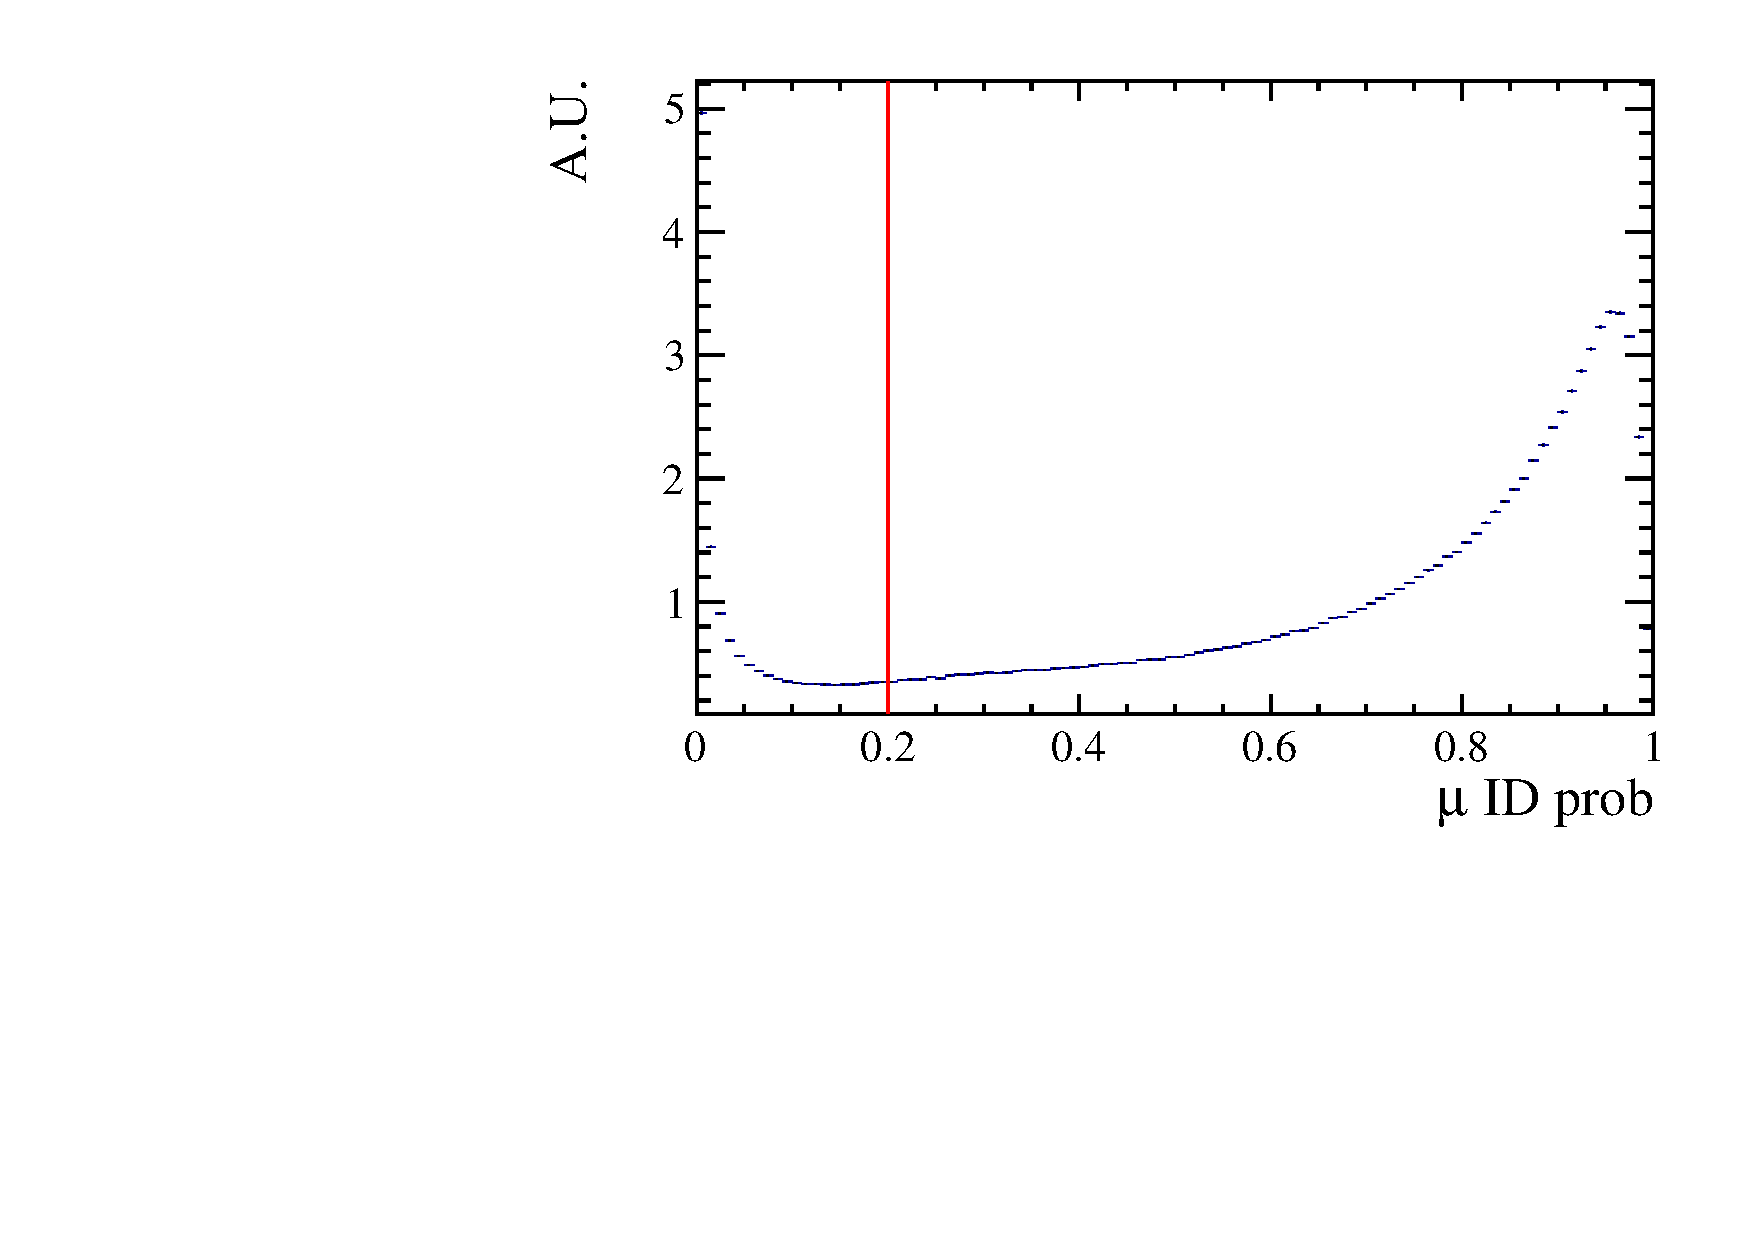
\includegraphics[width=0.48\textwidth]{RKst/figs/muon_PID.pdf}
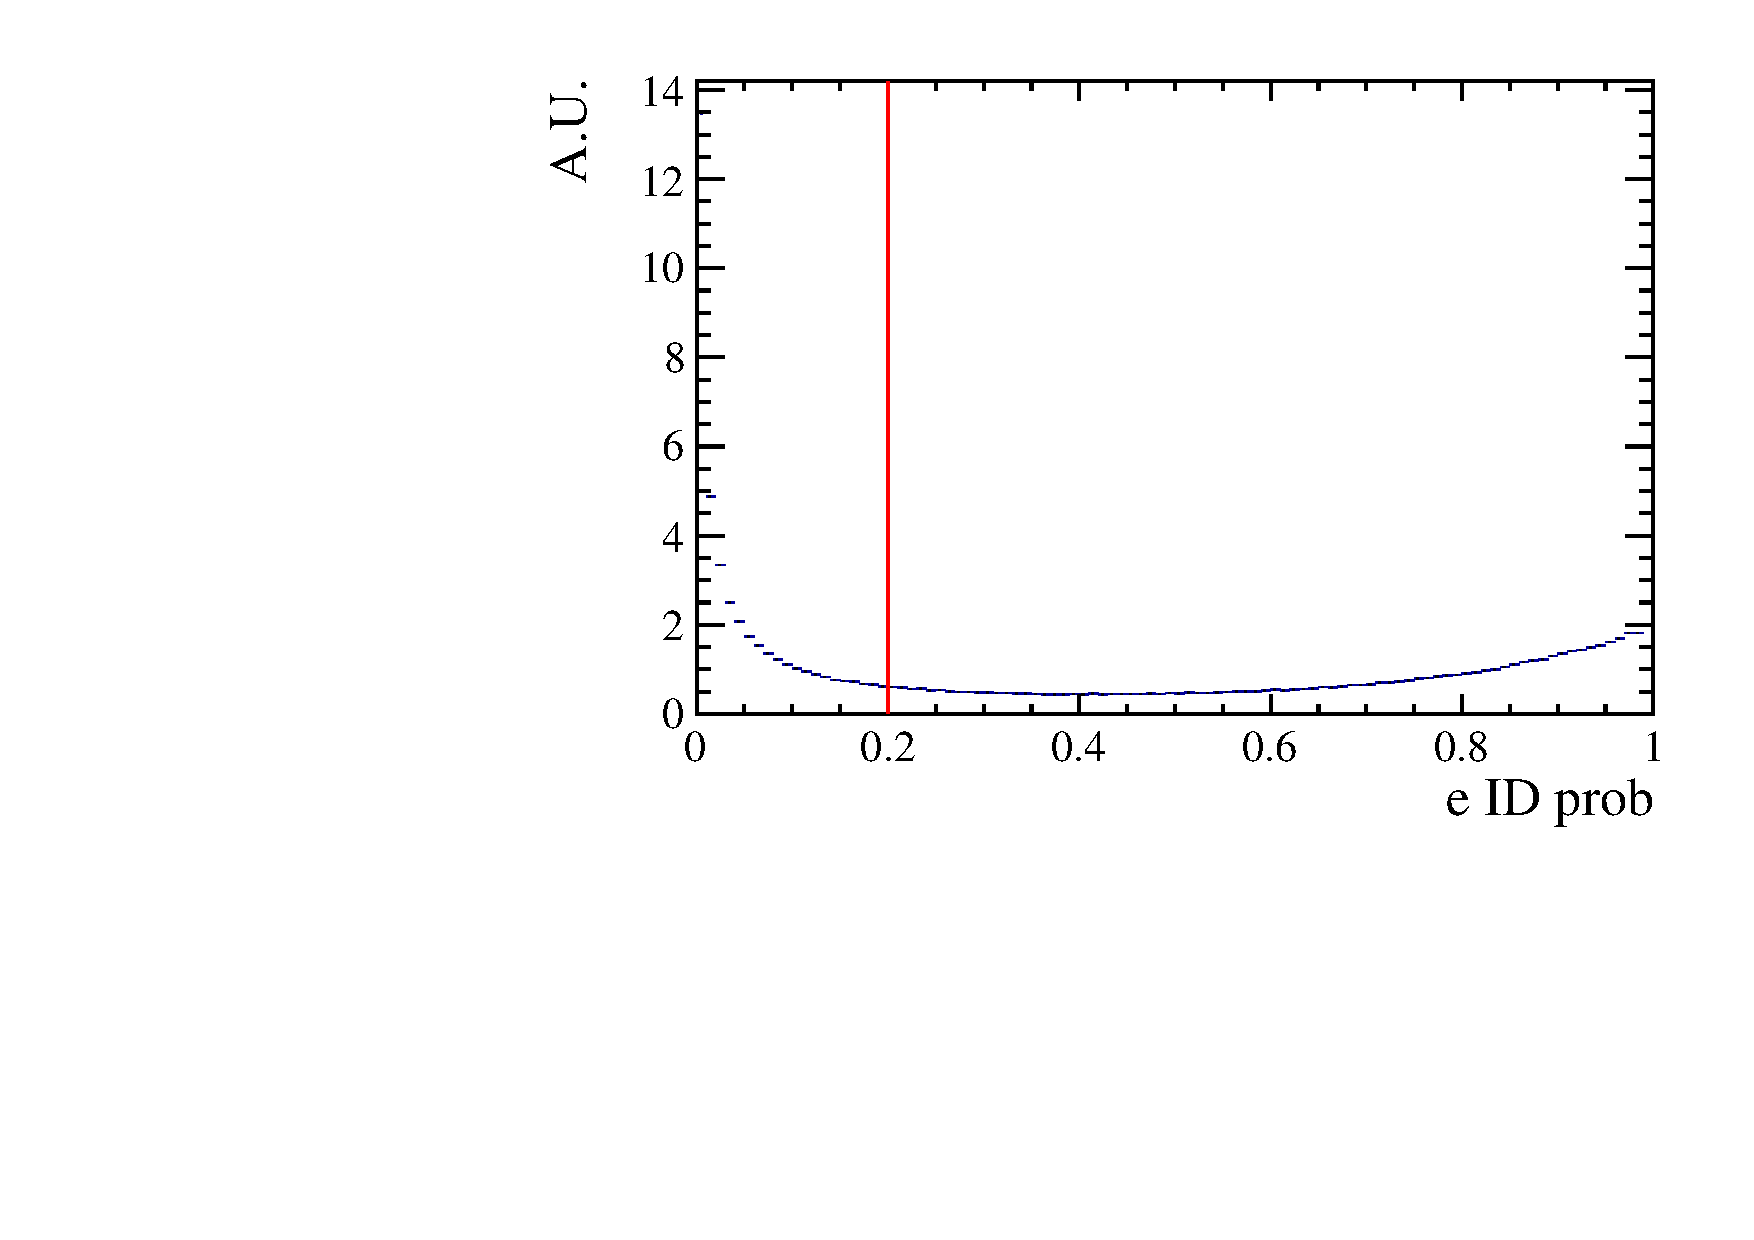
\includegraphics[width=0.48\textwidth]{RKst/figs/electron_PID.pdf}
\caption{Correct ID probability distributions for muons (left)
and electron (right) in 2012 data.}
\label{fig:e_mu_pid}
\end{figure}
%
\begin{figure}[h!]
\centering 
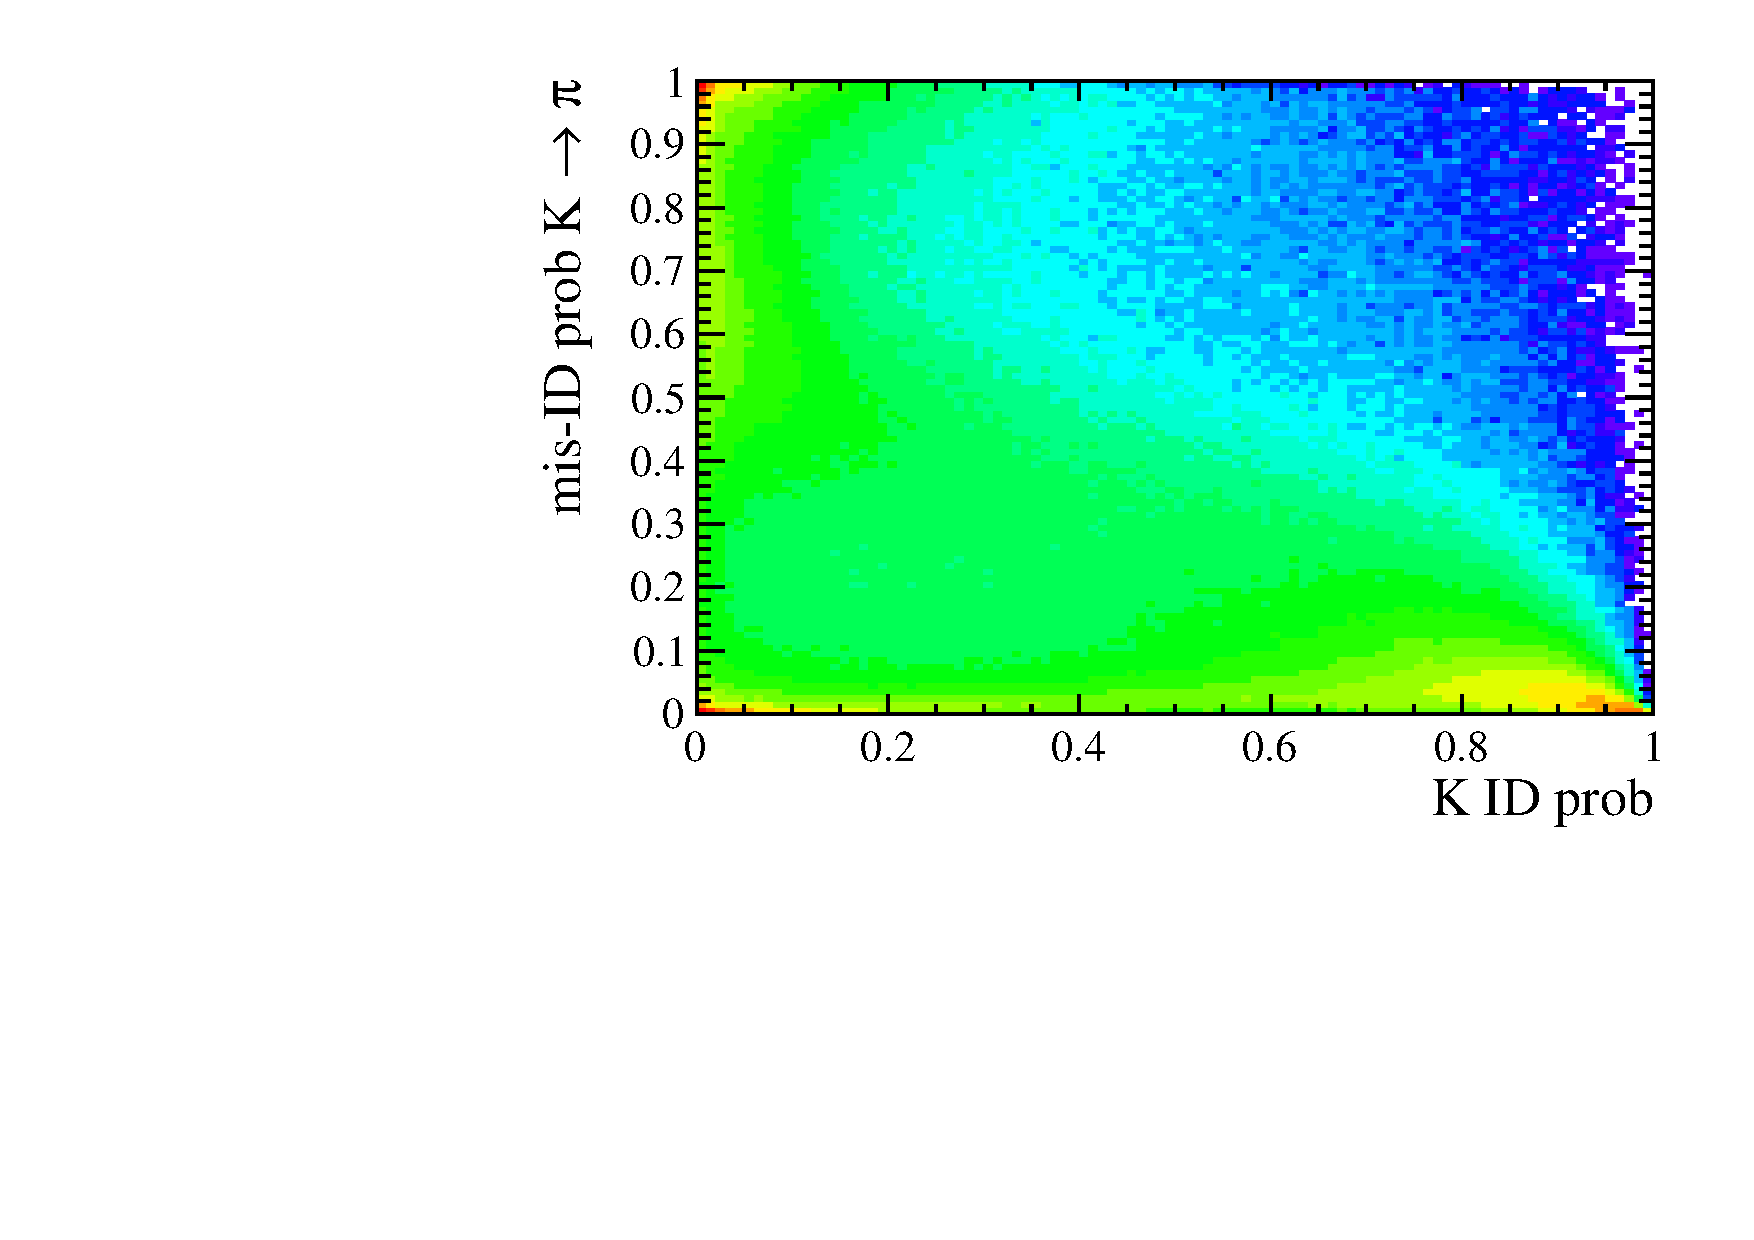
\includegraphics[width=0.48\textwidth]{RKst/figs/kaon_PID.pdf}
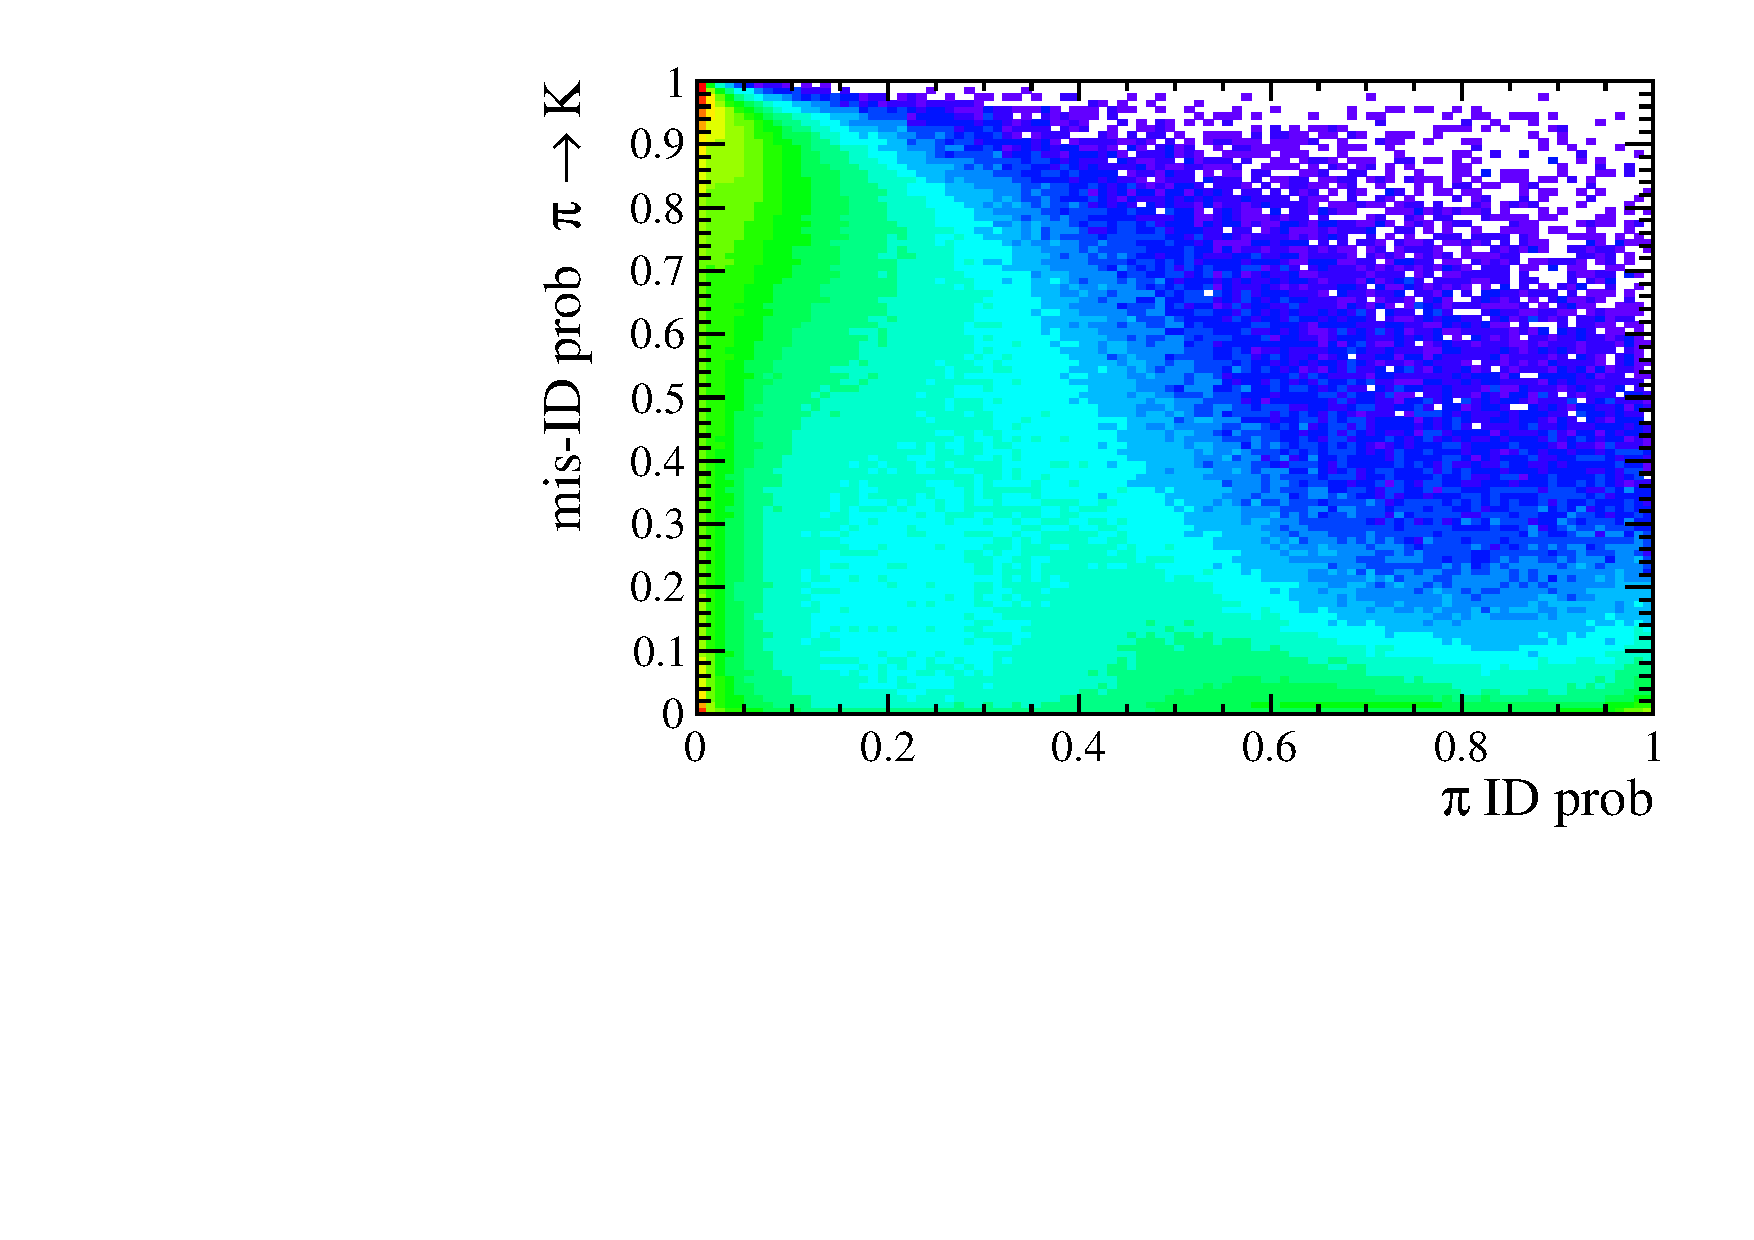
\includegraphics[width=0.48\textwidth]{RKst/figs/pion_PID.pdf}
\caption{On the horizontal axis of these plots is shown the correct ID
probabilities for kaons (left) and pions (right),
 while the vertical axes show the mis-ID probabilities.}
\label{fig:k_pi_pid}
\end{figure}

Figure~\ref{fig:e_mu_pid} shows probability distributions, {\verb ProbNNe } and {\verb ProbNNmu },
for the electrons and muons in the decay candidates, while Fig.~\ref{fig:k_pi_pid} shows the probabilities 
of correct identification and mis-identification of kaons and pions in a two-dimensional plane.
These plots are characterised by clear peaks at maximal ID probability and minimal mis-ID
probability, corresponding to particles to which a well defined identification can be assigned.
%
In order to maximise the power of the PID requirements, the probabilities for correct ID 
and mis-ID are combined and requirements imposed as:
%
\begin{center}
\begin{tabular}{lcl}
$\pi$     & \to  & $\verb!ProbNNpi! \times (1 - \verb!ProbNNk!) \times (1 - \verb!ProbNNp!) > 0.1$ \\
$K$      & \to  & $\verb!ProbNNk! \times (1 - \verb!ProbNNp! ) > 0.05$ \\ 
$\mu$  & \to  & $\text{min}(\verb! ProbNNmu!(\mu_1) , \verb! ProbNNmu!(\mu_2)\;) > 0.2$  \\
$e$      & \to  & $\text{min}(\verb! ProbNNe!(e_1), \verb! ProbNNe!(e_2)\;) > 0.2$ \\
%$\pi$ &\to  & $\verb!ProbNNpi-V3! \times (1 - \verb!ProbNNk-V2!) \times (1 - \verb!ProbNNp-V2!) > 0.1$ \\
%$K$   &\to  & $\verb!ProbNNk-V3! \times (1 - \verb!ProbNNp-V2! ) > 0.05$ \\ 
%$\mu$ &\to  & $\text{min}(\verb! ProbNNmu-V3! , \verb! ProbNNmu-V3 !) > 0.2$  \\
%$e$   &\to  & $\text{min}(\verb! ProbNNe-V3! , \verb! ProbNNe-V3 !) > 0.2$ \\
\end{tabular}
\end{center}
%
In the first formula, for example, {\verb ProbNNpi } is the probability of correctly identifying the
pion as a pion, while {\verb ProbNNk } is the probability of mistaking it for a kaon.
Therefore by maximising the quantity ``{\verb ProbNNpi } $\times$ (1 - {\verb ProbNNk })",
one can maximise the correct ID probability and minimise at the same time the mis-ID probability.
In this example, the probability for mistaking the pion as a proton is also used.
%In the kaon case we do not use requirements on the $K\to\pi$ mis-ID probability
%because this cut was found to be unacceptably inefficient.


\subsection{Peaking backgrounds }

Backgrounds due to specific decays usually peak in some variable because of their
distinctive kinematic properties and therefore they can be removed without significant
efficiency loss for the signal. The following sections describe the main sources of peaking background.
The same requirements are applied to the muon and electron channels, unless stated otherwise.

\subsubsection{Charmonium vetoes}

Charmonium resonances such as \jpsi and \psitwos peak in \qsq.
The choice of \qsq binning described in Sec.~\ref{sec:RKst_q2_choice}
constitutes a natural veto for these decays. Simulated events are used
to check if resonant candidates leak inside the \qsq intervals chosen for
the rare channel analysis. For the muon channels the leakage is negligible
as the peaks are sharper due to the better momentum resolution and because muons 
emit fewer bremsstrahlung photons, resulting in shorter radiative tails.
The electron channels are characterised by a poorer energy resolution and an increased 
radiation of bremsstrahlung photons, yielding long tails at low \qsq.
Analysing simulated events it was found that 1.3 -- 2\% (depending on
the trigger category) of \mbox{$\Bz\to\Kstarz(\jpsi\to\ee)$} candidates leak into the 
$1.1 < \qsq < 6$~\gevgevcccc interval and 1.8\% of \psitwos events leak above 
15~\gevgevcccc. The contribution from these candidates is modelled in the fit. 


\subsubsection{$\phi$ veto}

A kaon from the decay $\Bs \rightarrow \phi \ll$, where the $\phi$ decays in two kaons,
can be mis-identified as a pion and therefore causes the $\phi$ to be reconstructed as a $\Kstarz$. This results in
a candidate with a value of $m(K\pi)$ that is less than the nominal \Kstarz mass but still high enough to
pass the selection requirements. Figure~\ref{fig:phiplots} (left) shows a plot of $m(K\pi)$ versus
$m(K\pi \mu\mu)$, where the kaon mass hypothesis is assigned to the pion. A peak can clearly be seen
around the (\Bs,$\phi$) mass.
To remove this background only candidates with $m_{K(\pi\rightarrow K)} > 1040$~\mevcc~are selected.
This results in a $\sim98\%$ background rejection while keeping a $\sim99\%$ signal efficiency.
%This cut could be further optimised using PID information. On the other hand LHCb simulation 
%struggles modelling the PID variables correctly. Therefore using PID in these cuts would
%add systematic uncertainties without significantly improving the signal efficiency which is already 99\%.
\Bs decays such as $B_s \rightarrow \phi \Kstarz$ could also constitute a background when the $\phi$ decays 
into two leptons but the branching fraction of this decay is small compared to the previous case.
Furthermore, this contribution is already taken into account by the choice of the \qsq intervals (see Sec.~\ref{sec:RKst_q2_choice}).

\begin{center}
\begin{figure}[h!]
\centering 
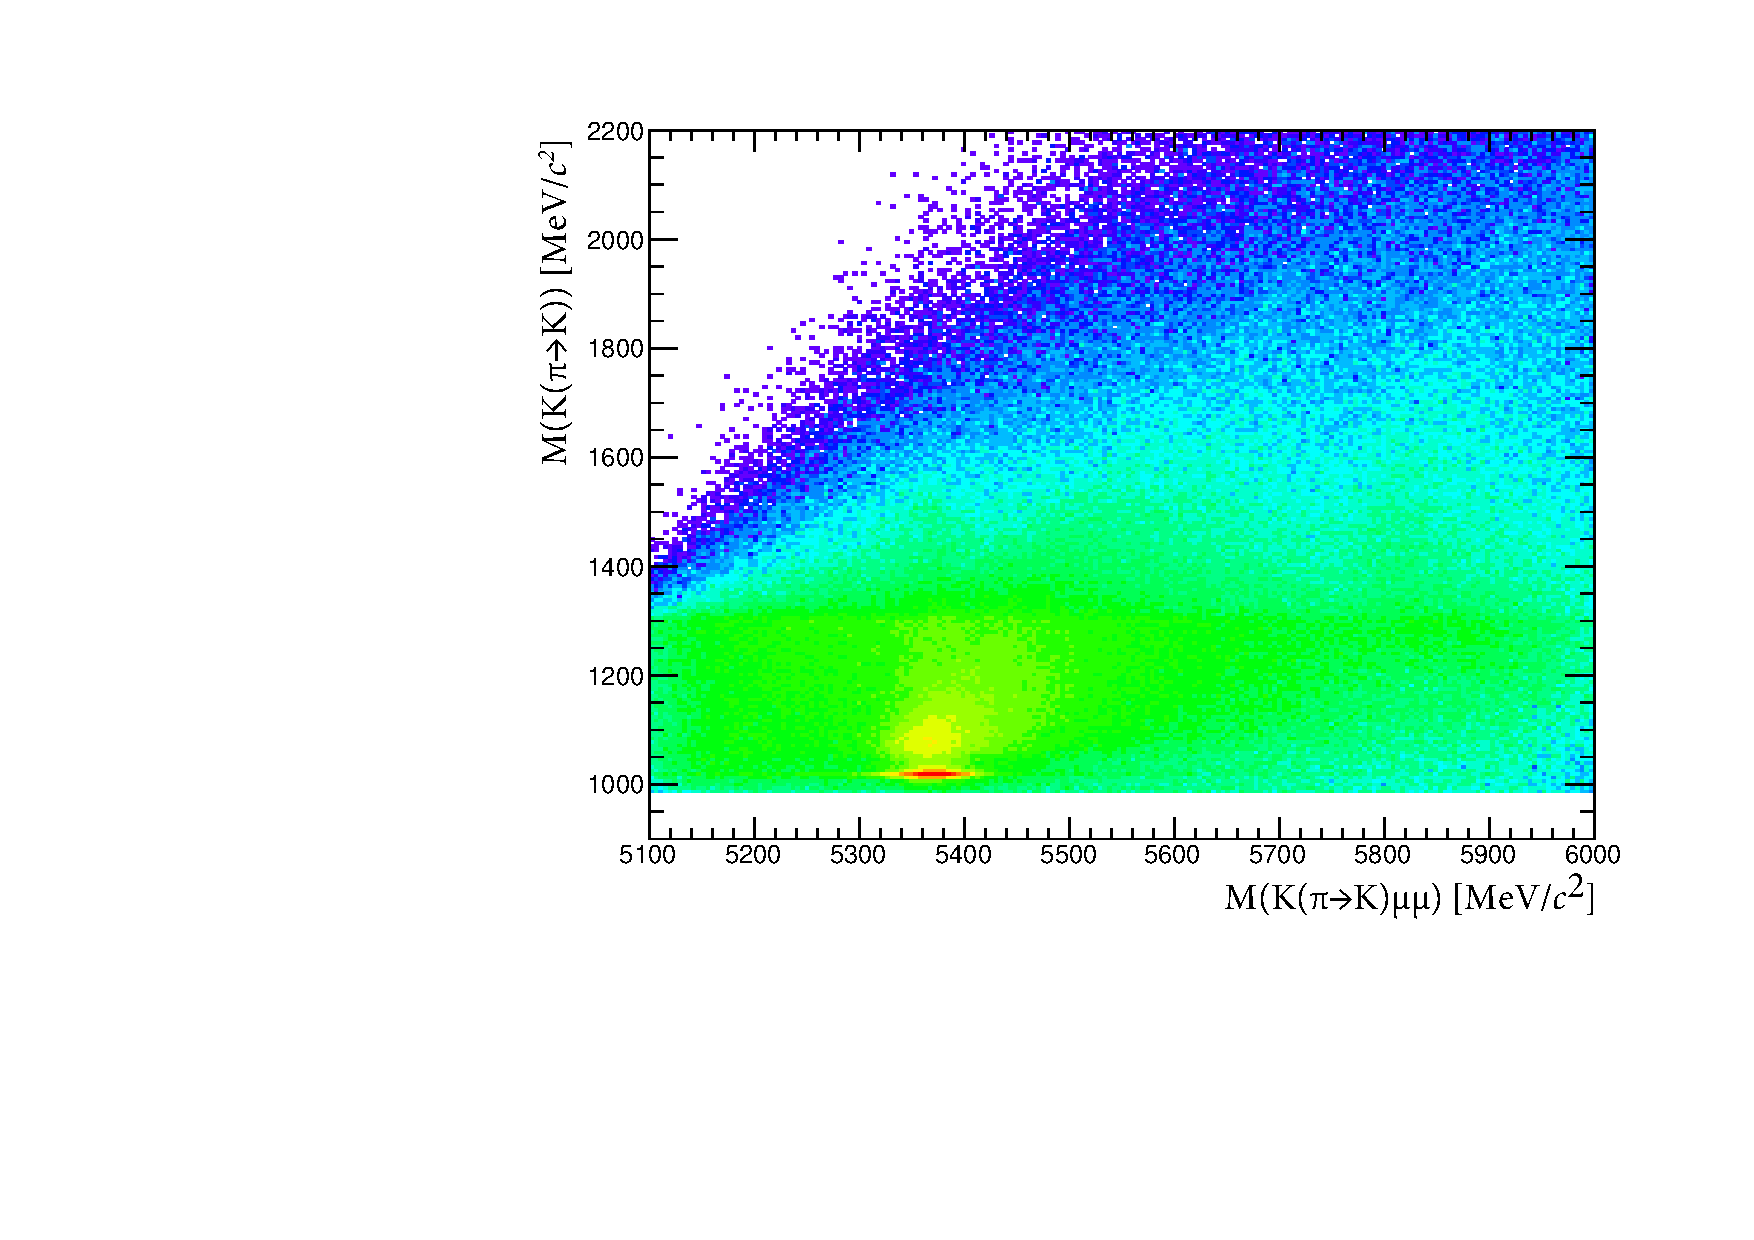
\includegraphics[width=0.49\textwidth]{RKst/figs/Background/phi.pdf}
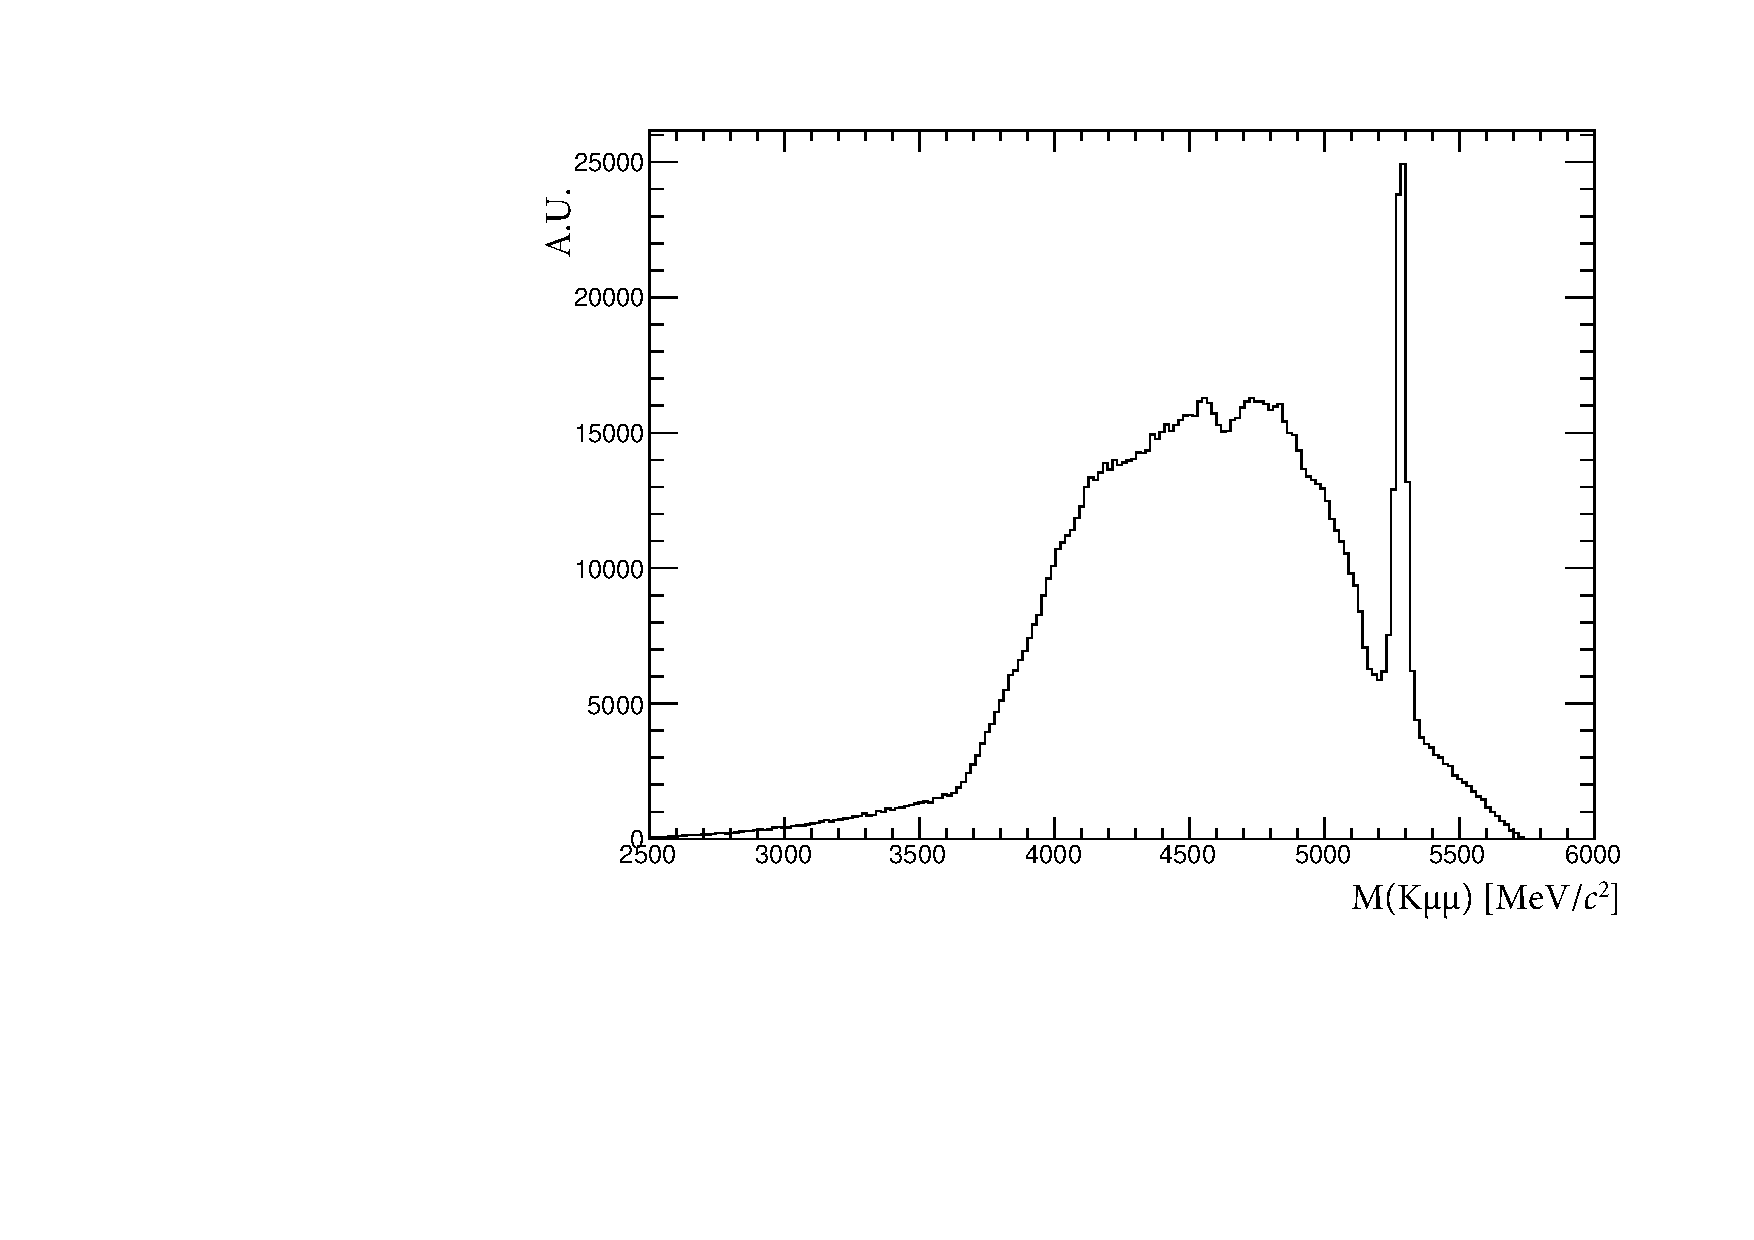
\includegraphics[width=0.49\textwidth]{RKst/figs/Background/Kmumu.pdf}
\caption{ (left) Distribution of data candidates as a function of the variables $(m_{K(\pi\rightarrow K)})$ 
and $(m_{K(\pi\rightarrow K)\mu\mu})$, where $\pi\rightarrow K$ means that the kaon mass hypothesis 
is assigned to the pion. (right) The invariant mass distribution of the three-body system $(K\mu\mu)$,
where the peak due to the $B^+ \to K^+ \mumu$ decay is visible. }
\label{fig:phiplots}
\end{figure}
\end{center}


\subsubsection{$\Bu \to K^+ \ll$ plus a random pion}

$\Bu \to K^+ \ll$ decays can contaminate the upper \Bz mass sideband if they are combined
with a soft pion from elsewhere in the event and therefore reconstructed as a \Bz decay.
Similarly a kaon can be mis-identified as a pion and combined with another kaon in the event.
Figure~\ref{fig:phiplots} (right) shows the invariant mass distribution of the three-body ($K\mumu$) system,
$m(K\mu\mu)$. This is characterised by a narrow peak at the $\Bu$ mass. Since these
candidates have $m(K\pi\ell\ell) > 5380$~\mevcc~there is no contribution under the \Bz peak,
but they can cause problems when using sidebands candidates to train the neural network.
An effective veto for this decay was found to be max$(m_{K\ell\ell},m_{(K\to\pi)\ell\ell}) < 5100$~\mevcc,
which results in a $\sim95\%$ background rejection while keeping $\sim99\%$ signal efficiency.

\subsubsection{$\Lambda_b$ decays}

$\Lb\to\jpsi\Lz$ decays are unlikely to be reconstructed as $\Bz \to \Kstarz \ll$ because
the \Lz is long-lived and decays further in the detector with a separate vertex.
%Nevertheless, simulated events were used to check how many 
The number of candidates falling into the \Bz samples was estimated using simulation and found to be negligible. 
In contrast, the $\Lb\to\jpsi pK$ decay channel can contribute more easily, when the proton is mis-identified as a kaon.
In fact, the $m(pK)$ is above the \Lz threshold and therefore they must come from $\Lz^*$ resonances, 
 which are not long-lived. This background is already reduced by the PID requirements but a non-negligible contribution 
 is still expected, and cannot be easily removed due to its broad shape. It is therefore modelled in the fit.

\subsubsection{\decay{\Bd}{(\Dm\to K \en \overline{\nu})\ep\nu} }

The \decay{\Bd}{\Dm\ep\nu} decay, where the \Dm in turn decays semileptonically to $\Kstarz\en\nu$ has the same final particles
as the \BdToKstee decay plus two neutrinos which are not reconstructed. This decay has a branching ratio four orders of magnitude
larger than \BdToKstee in the low-\qsq region and it may pass the selection requirements when the two neutrinos have low momentum. 
%This cut, developed for the angular analysis, 
To reduce the level of this background the angle $\theta_\ell$ is used, which is defined as the angle between the direction of the \ep (\en)
in the di-electron rest frame and the direction of the di-electron in the \Bd (\Bdb) rest frame. 
Low momentum neutrinos demand the \Dm and the \ep to be almost back-to-back in the \Bd rest frame giving the \ep a relatively
high energy compared to the \en. As a consequence, the direction of the \ep is close to the direction of the di-electron pair, thus the
$\theta_\ell$ angle is close to zero. In fact the distribution of background candidates, obtained imposing the invariant mass cut
$m(K\pi ee) < 4800$~\mevcc, is asymmetric towards extreme $\cos \theta_\ell$ values as it can be seen in Fig.~\ref{fig:Denu_background}. 
The requirement $|\cos \theta_\ell\,|< 0.8$ is used but is not applied in the high-\qsq case as the variable has reduced discriminating power.
%The percentage of \BdToeeKst signal events lost applying this cut is quite low, about $10\%$ according to MC. 
In the muon channels, the background from \decay{\Bd}{(\Dm\to K \mun \overline{\nu})\mup\nu} decays remains outside 
of the invariant mass window used for the fits.

\begin{figure}[t!]
\centering
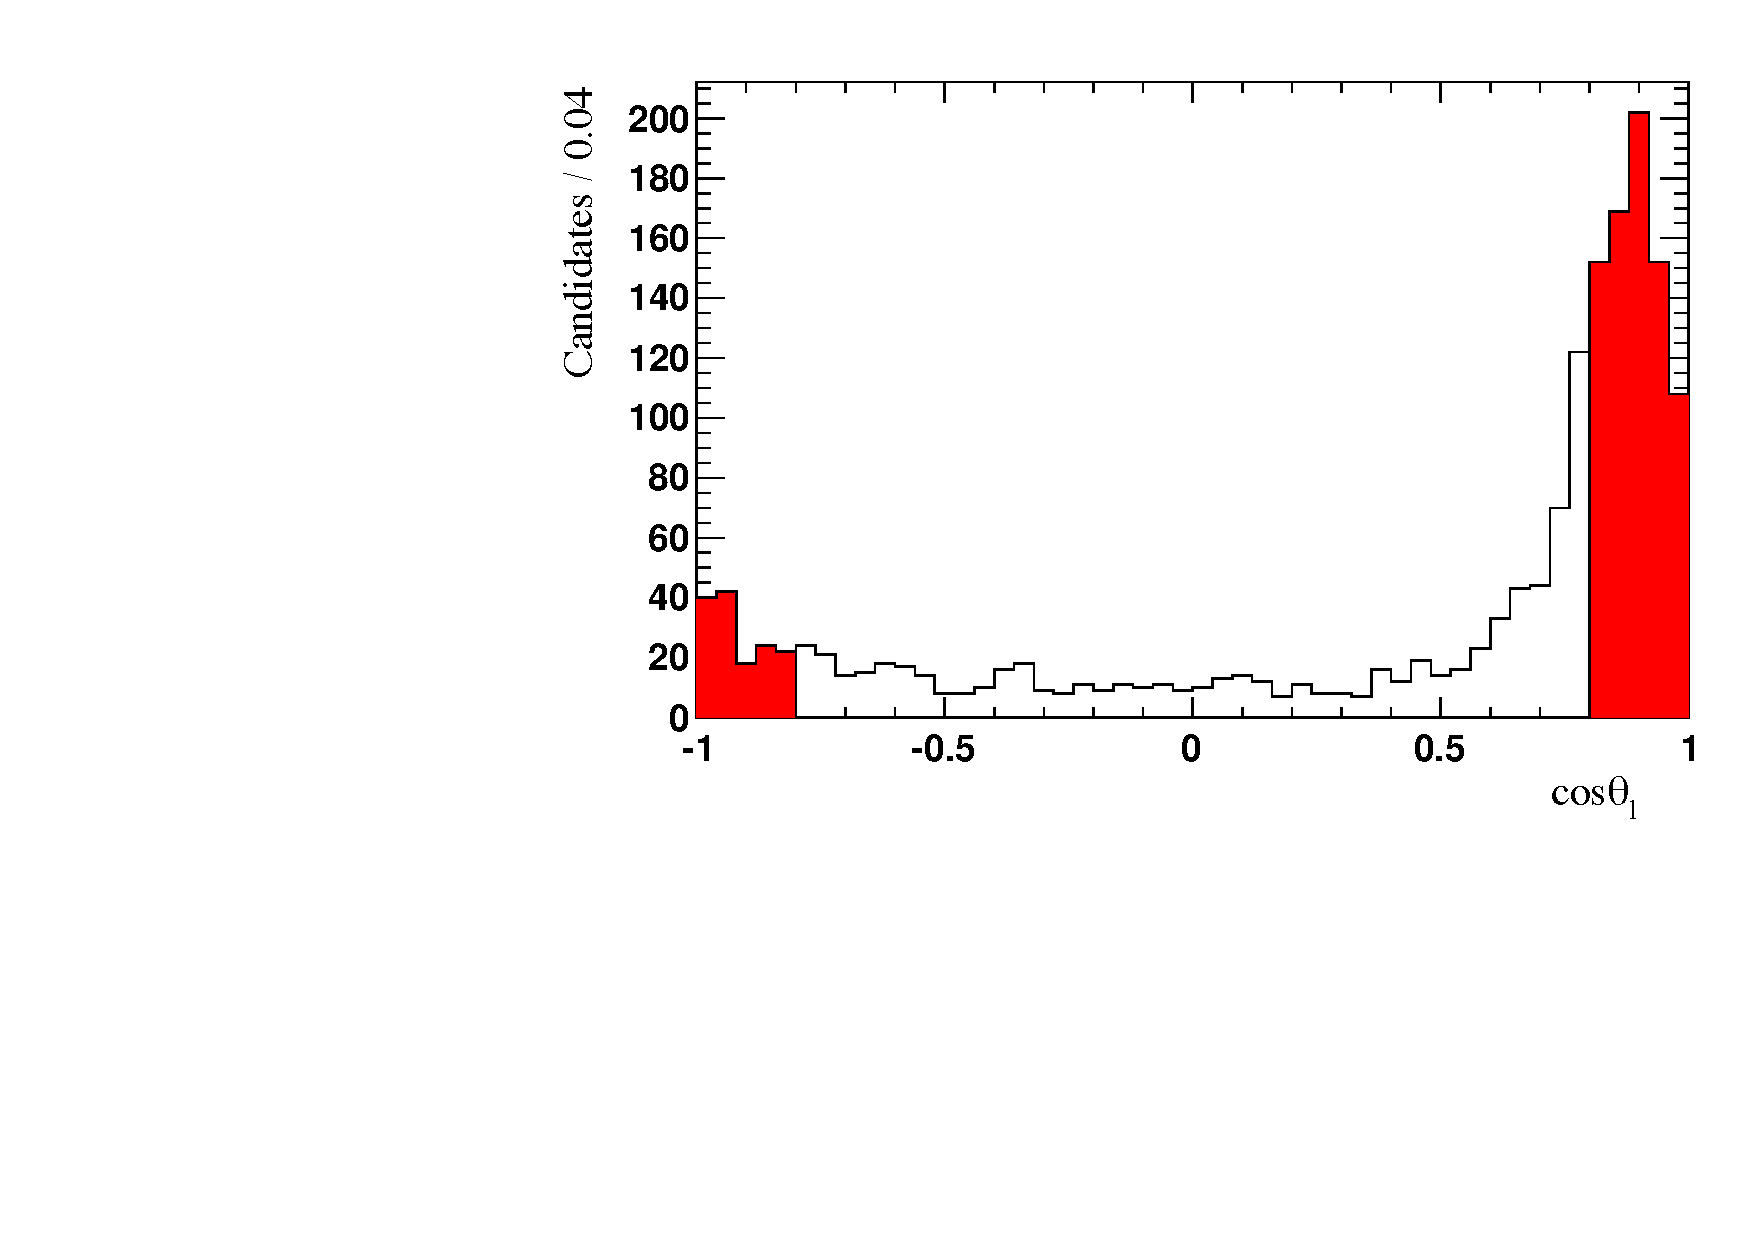
\includegraphics[width=0.49\textwidth]{RKst/figs/misreco/CosThetaL_background.pdf}
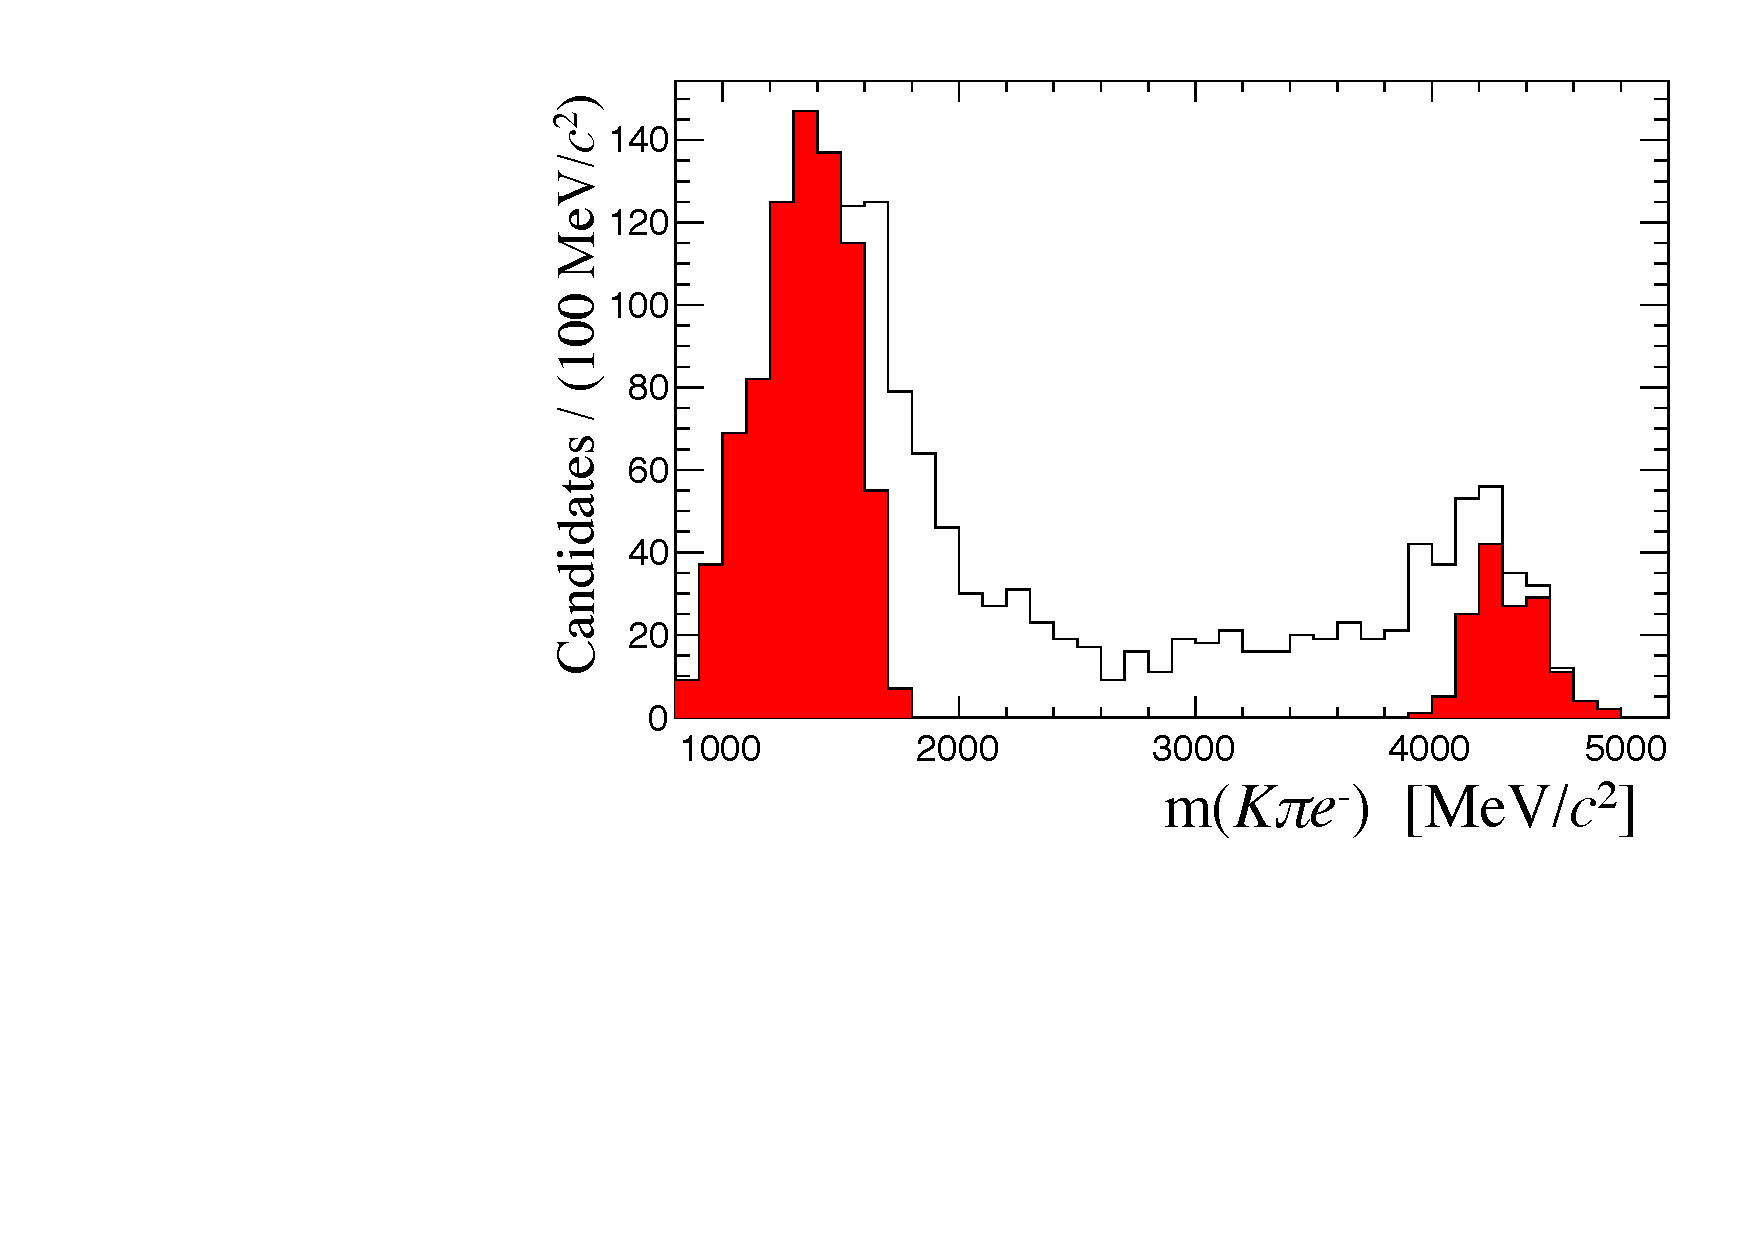
\includegraphics[width=0.49\textwidth]{RKst/figs/misreco/KstareMass_background.pdf}
\caption{Distribution of (left) $\cos \theta_\ell$ and of (right) the $m(K\pi e^-)$ invariant mass, where the \decay{\Bd}{(\Dm\to K \en \overline{\nu})\ep\nu} background is selected by requiring $m(K\pi ee) < 4800~\mevcc$. The red distribution highlights candidates with $| \cos \theta_\ell\,| > 0.8$.}
\label{fig:Denu_background}
\end{figure}

\subsubsection{\BdToKstGee}

For the low-\qsq region, a potentially dangerous peaking background is due to the \BdToKstG decay followed by a conversion
of the photon in the detector. The branching fraction of \BdToKstG has been measured to be \mbox{\BF~= $(4.33 \pm 0.15)\times 10^{-5}$} and, 
when the photon converts to an electron and a positron, has similar characteristics to \BdKstee. 
In \lhcb around 40\% of photons convert before the calorimeter. Although only $\sim 10\%$ of these convert
in the VeLo and are reconstructed as long tracks, the resulting \Bd mass should peak under that of the signal. 
This signal-like background is reduced effectively by the choice of the lower bound for the low-\qsq interval which corresponds to 
$m(ee)=20$~\mevcc. Furthermore, the \ee~pair from \BdToKstGee has a vertex at the point where the photon converts, but it may 
still be reconstructed as originating from the \Bd decay if the \ee~vertex position is determined with a large uncertainty. 
Therefore a requirement is applied on the uncertainty of the reconstructed $z$-coordinate of the \ee~pair: $\sigma_z(\ee) < 30$~mm.
%The contamination from the background is estimated in the following way: a quasi pure sample of \BdToKstGee is selected requiring that the 
%reconstructed invariant mass window for the \epem pair is smaller than 5~\mevcc. The event yield obtained on data ($881 \pm 39$ events)
%s used to rescale the prediction of the LHCb MC to get rid of problems related to an absolute prediction. 
Simulated events are used to predict the contamination from \BdToKstGee decays in the signal region which is found to be $(3.2\pm1.6)\%$.
%1.6 \%. 
%Finally as pointed out in ~\cite{LHCb-ANA-2014-009}, a conservative correction to take into account the mis-modelling 
%of the Bethe-Heitler process in Geant4 is further applied. The contamination is estimated to amount to  $(3.2\pm1.6)\%$ of the signal yield. 



\subsubsection{Other peaking backgrounds}

%A possible background could come from $\Bz \to\Kstarz\gamma$ decays where the photon converts
%into two electrons while traversing the detector. In LHCb, around 40\% of photons convert before the calorimeter,
%but only a small fraction of these, $\sim 10\%$, are reconstructed. Furthermore these events fall
%into a \qsq region well below the intervals considered in this analysis and their contribution is therefore negligible.

A potential contamination from $\Bz \to\Kstarz\eta$ and $\Bz \to\Kstarz\pi^0$, where the $\eta$ and the pion decay into
two photons, was considered and found to be small.
Furthermore, a potentially dangerous background could come from candidates where the
identity of the kaon and the pion are swapped as these candidates peak under the signal.
Although their contribution is found to be small, 0.5\%, the effect of their modelling in the fit
is taken into account when evaluating the systematic uncertainties. Finally, charmonium decays where 
the identity of the kaon, or the pion, and one of the muons  are swapped is are rejected by requiring that the 
hadron-$\mu$ invariant mass $m((h \to \mu)\mu)$, where the muon mass hypothesis is assigned to the hadron, 
is not compatible with a \jpsi (\psitwos) resonance: $|m((h\to \mu)\mu)-m_{\jpsi, (\psitwos)} | > 60$~\mevcc.

\subsection{Partially-reconstructed background}
\label{sec:RKst_peaking_Dchains}

Partially-reconstructed candidates are defined as decays where one or more particles in the final state are not reconstructed,
resulting in $m(K\pi\ell\ell)$ values smaller than the mass of the \Bz, but with tails that can still contaminate the signal sample.
Sources of partially-reconstructed background are decays involving higher hadronic states such as 
\decay{\Bz}{(Y\to\kaon\pi X)(\jpsi\to\epem)}, where $X$ represents at least one particle that is not reconstructed. 
The $Y$ state can be a \Kstar resonance as well as \D mesons that decay semileptonically, as explained in the previous sections.
For the resonant channels, an additional source of partially-reconstructed 
background comes from decays of higher \ccbar resonances, \decay{\Bz}{(\Kstarz\to K\pi)(Y\to(\jpsi\to\epem)X)}.

To reject such backgrounds, the 4-body invariant mass $m(K\pi\ell\ell)$ is recalculated using 
\verb!DecayTreeFitter! to impose vertex constraints. For the resonant case this also includes constraining the invariant mass 
mass of the dilepton pair to that on the \jpsi; in this case the 4-body mass is denoted as $m(K\pi\ell\ell)_{\jpsi}$. This constraint 
pushes partially-reconstructed candidates towards low $m(K\pi\ell\ell)_{\jpsi}$ values, resulting in no contamination above 5150~\mevcc. 

This requirement is implicitly applied for the muon channels by the definition of the invariant mass fit-windows. For the electron channels,
the requirement $m(K\pi\ell\ell)_{\jpsi(\psitwos)} > 5150~\mevcc$ is explicitly applied to select the $\jpsi(ee)$ and $\psitwos(ee)$ samples.
However, the vertex constraint alone is not sufficient to remove all background in the electron rare decay channels.
Furthermore, to correctly model the long radiative tails of the mass shapes, a fit region that extends 
down to 4500~\mevcc~is necessary. As a consequence the partially-reconstructed background is still relevant
for the electron rare channels and extends below the signal peak. For this reason this background is modelled 
in the fit for the rare channels (for details see Sec.~\ref{sec:RKst_misreco_fit}).


%Mis-reconstructed background is defined as decays where one or more particles are not reconstructed.
%The candidates built from these decays tend to have a low 4-body invariant mass as some particles are not reconstructed.
%A source of mis-reconstructed background is due to cascade decays with a \Bz decaying semileptonically
%into a $D$ meson which also decays semileptonically, e.g. $\Bz\to D^{-} \ell^+ \bar{\nu_\ell}$
%followed by $D^{-} \to \Kstarz \ell^- \nu_\ell$. 
%This is in general true for any partially reconstructed background from $B$ decays.
%
%To remove this background in the muonic channels, the 4-body $m(K\pi\mumu)$ invariant mass is recalculated
%with a kinematical fit using the \verb!DecayTreeFitter! package. In the resonant case this includes a constraint of the dilepton
%mass to be the \jpsi nominal mass and in both rare and resonant cases each particles is constrained to point to 
%its origin vertex. This constraint has the effect of pushing the misreconstructed events far from the \Bz peak.
%Therefore, to avoid this background, it is sufficient to limit the analysis to 4-body invariant masses
%above 5150~\mevcc.

%In the electron case it is instead important to fit a wider mass window to correctly constrain the background
%therefore one cannot eliminate this mis-reconstructed background which is then modelled in the fit
%(for details see Sec.~\ref{sec:RKst_misreco_fit}).

\subsection{Bremsstrahlung corrected mass}
\label{sec:HOP}

For the electron channels it is particularly difficult to separate partially-reconstructed and combinatorial background from the 
long radiative tail of the signal. Additional information to reduce these backgrounds is provided by the kinematics of the decay: 
the transverse momentum of the \Kstarz and dielectron, defined relative to the flight direction\footnote{The flight direction is defined 
using the primary and the decay vertices.} of the parent \Bz meson, should be equal and opposite, as illustrated in Fig.~\ref{fig:schemaHOP}.
%\cite{LHCb-INT-2015-000}.
%In fact for the \Bz daughters, the \Kstarz and the dielectron, the momentum components orthogonal to the flight 
%direction\footnote{The flight direction is defined using the primary and the decay vertices.} of the \Bz meson, \pt, 
%should cancel out as described by the sketch shown in Fig.~\ref{fig:schemaHOP}.
\begin{figure}[b]
 \centering
    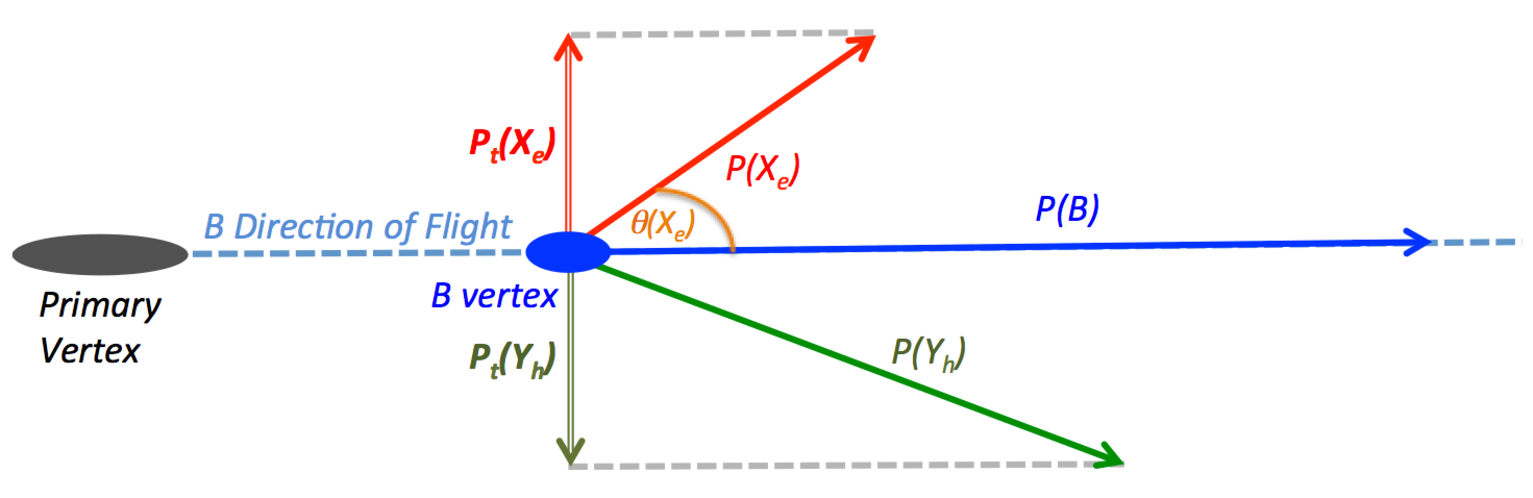
\includegraphics[width=0.9\linewidth]{RKst/figs/HOP/schemaHOP.pdf}
  \caption{ Schematic of the kinematic of a $B \to Y_h X_e$ decay, highlighting the quantities relevant for the 
  definition of the bremsstrahlung correction factor, $\alpha$.}
  \label{fig:schemaHOP}
\end{figure}

The ratio between the transverse momenta, \pt, of the \Kstarz and the dielectron pair, $\alpha = \pt(\Kstarz) / \pt(\ee)$, can be used 
to check this hypothesis. When $\alpha$ deviates from one, some energy is missing in the final state. 
For signal candidates, the missing energy is most likely carried away by bremsstrahlung photons emitted
by the electrons. Therefore we can use $\alpha$ to correct the electron momentum as $\ptot_{\textrm{corr}}(\ee) = \alpha \cdot \ptot(\ee)$.
Since bremsstrahlung photons are predominantly emitted in the direction of the electron, the same $\alpha$ correction can
be also applied to the longitudinal component of the dielectron momentum.
In contrast, the missing particles in partially-reconstructed background candidates are not necessarily emitted in the
direction of the electrons, and therefore this correction does not work properly.
A similar argument applies to the combinatorial background. 

The corrected momenta can be used to re-calculate the invariant mass of the \Bz candidate, which in the following will be
called Bremsstrahlung Corrected Mass, \mbcm. The resolution of \mbcm depends on the quality of the vertex reconstruction
and on the \Bz lifetime, and degrades as a function of \qsq. Figure~\ref{fig:hop} shows the dependence of the \Bz $\chisq_{\rm FD}$ 
(flight distance $\chisq$) as a function of \mbcm in the considered \qsq regions. 

As the correction factor is not meaningful for backgrounds this leads the candidates to spread out making \mbcm 
a discriminating variable between signal and background. A two-dimensional cut is adopted
%
$$\mbcm > a_{\rm BCM} + b_{\rm BCM} \cdot \log(\chisq_{\rm FD}),$$
%
where the $a_{\rm BCM}$ and $b_{\rm BCM}$ coefficients are optimised as described in Sec.~\ref{sec:optimisation}.
%
No cut is applied either at high-\qsq because the variable loses discriminating power or to the muon 
channels for which the bremsstrahlung radiation is negligible.

%Figure~\ref{fig:hop2} shows the dependence of \mKpiee as a function of \mbcm in the considered \qsq regions. 

%The efficiency of the cut in the different bins of \qsq and for the different signal and background components is shown
%in Fig.~\ref{}. The cut efficiency is almost flat for the signal while it's rejection power is higher for low $B$ mass. 

%It should be noted that \mbcm has also a dependence on \qsq, as for high-\qsq the transverse momentum of the \Kstar, and consequently \hop, is less precisely determined.
%As a consequence, the cut turns out to be inefficient for the high-\qsq bin, where therefore it is not applied.
%No \hop requirement is used for the muon channels for which the bremsstrahlung is negligible. 

\begin{figure}[t!]
\centering
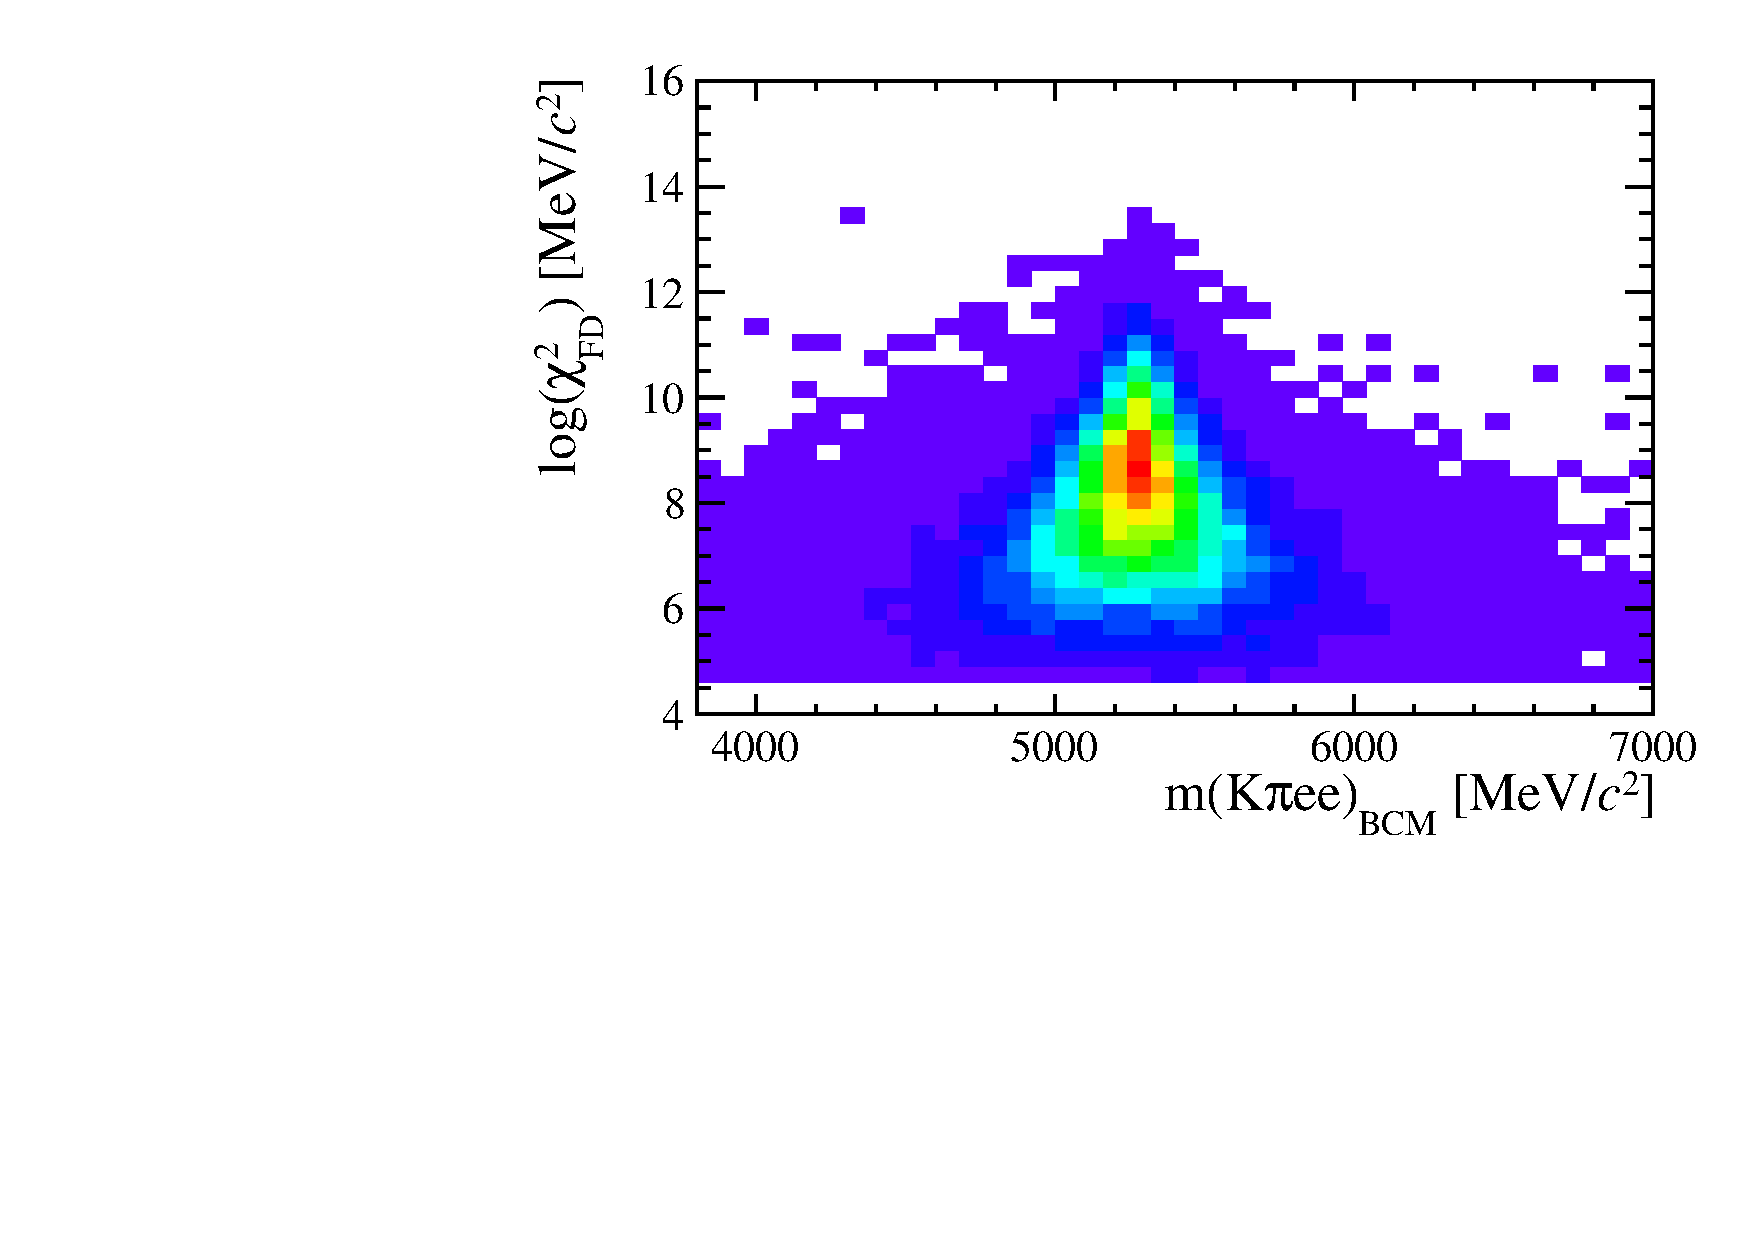
\includegraphics[width=0.48\textwidth]{RKst/figs/HOP/HOP_sig_low.pdf}
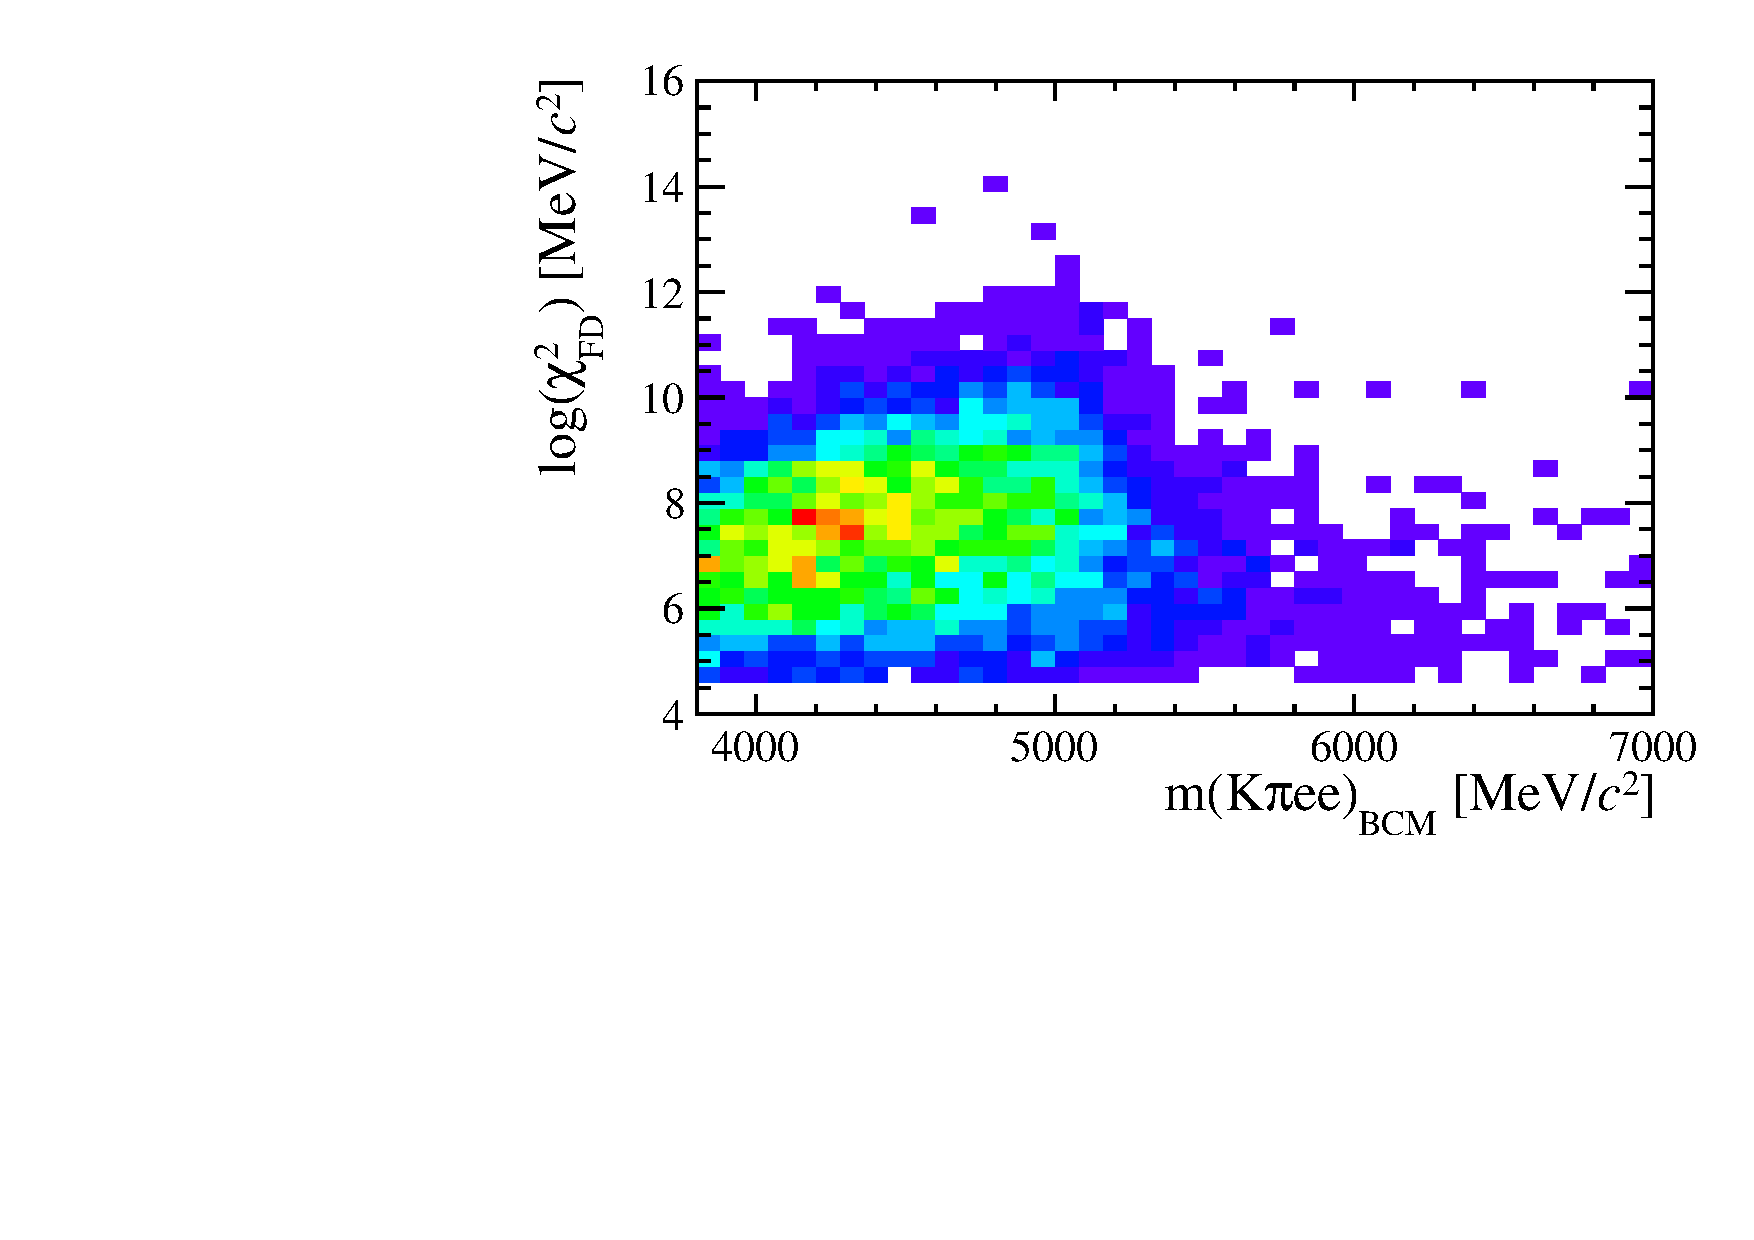
\includegraphics[width=0.48\textwidth]{RKst/figs/HOP/HOP_bkg_low.pdf}
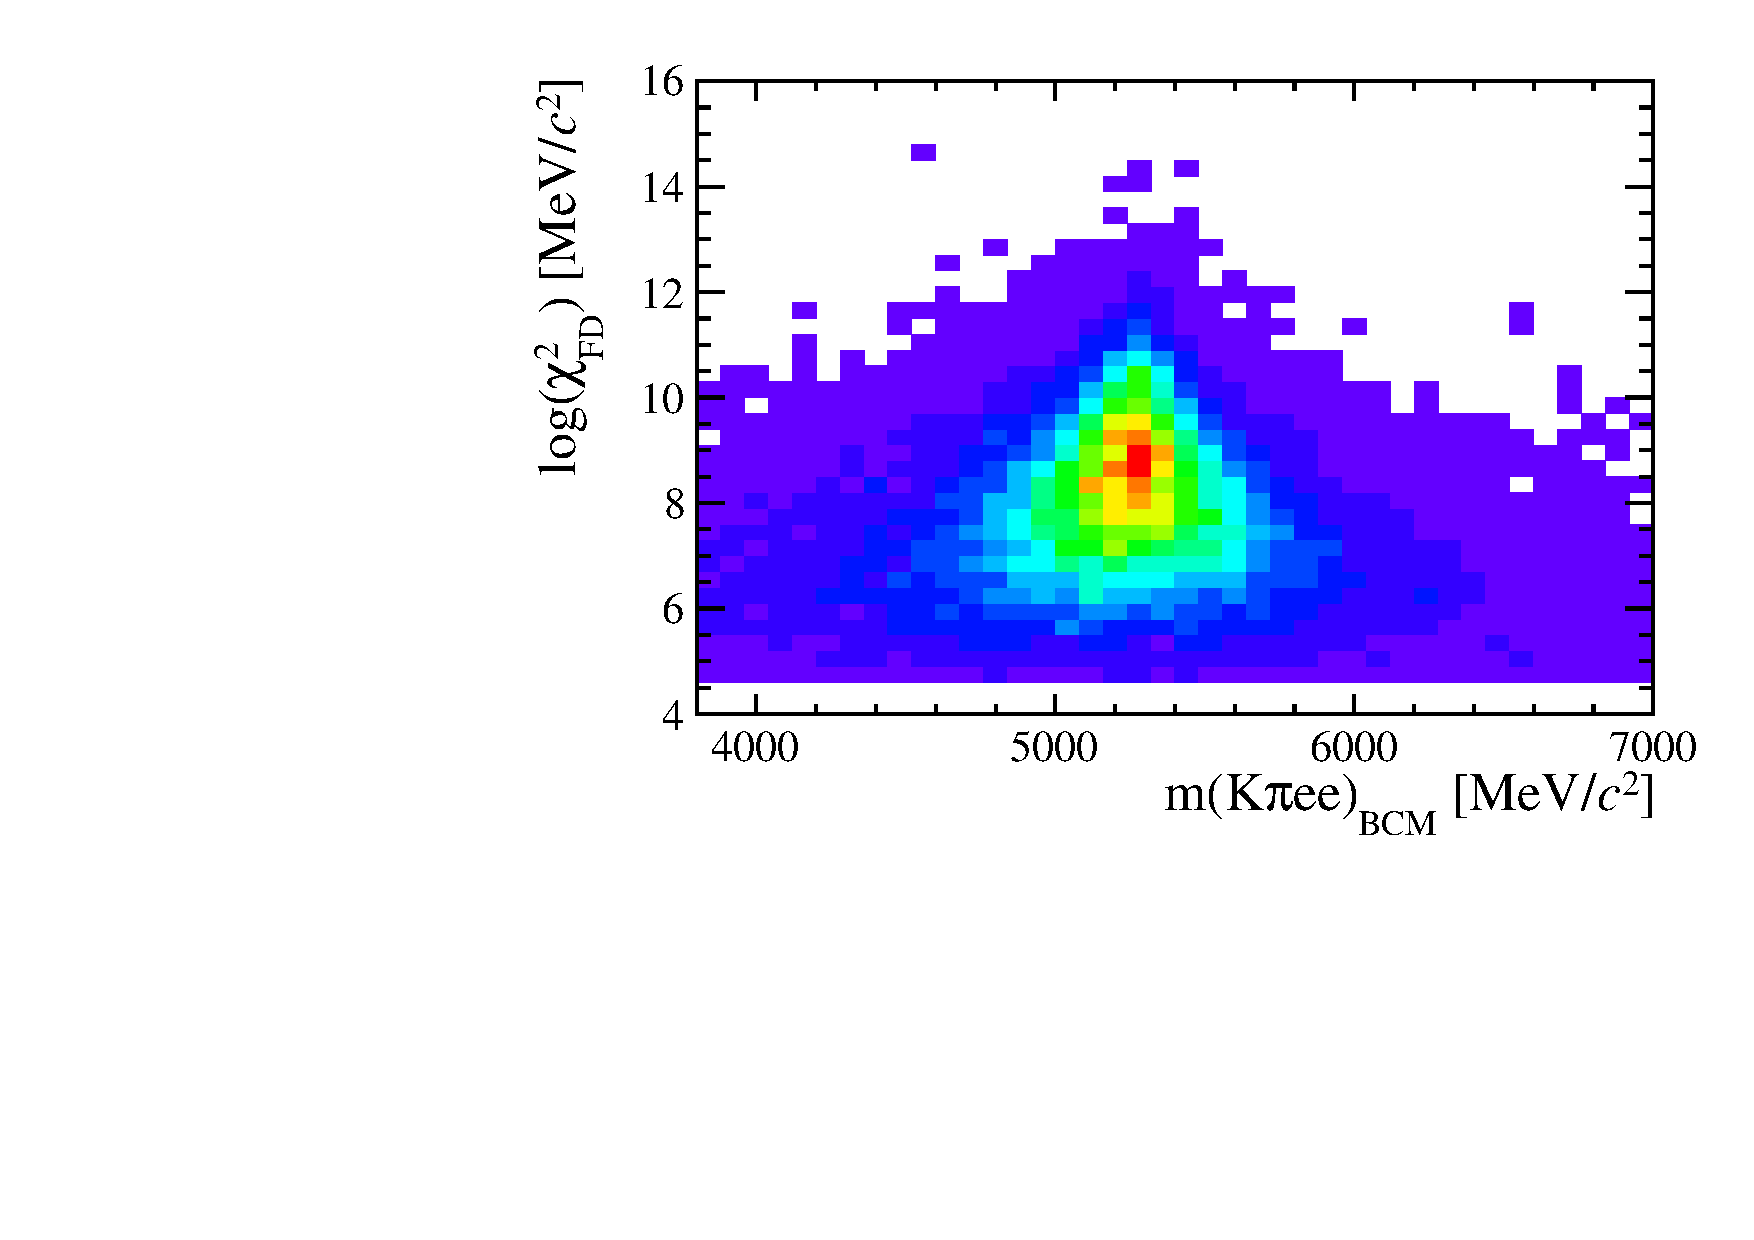
\includegraphics[width=0.48\textwidth]{RKst/figs/HOP/HOP_sig_central.pdf}
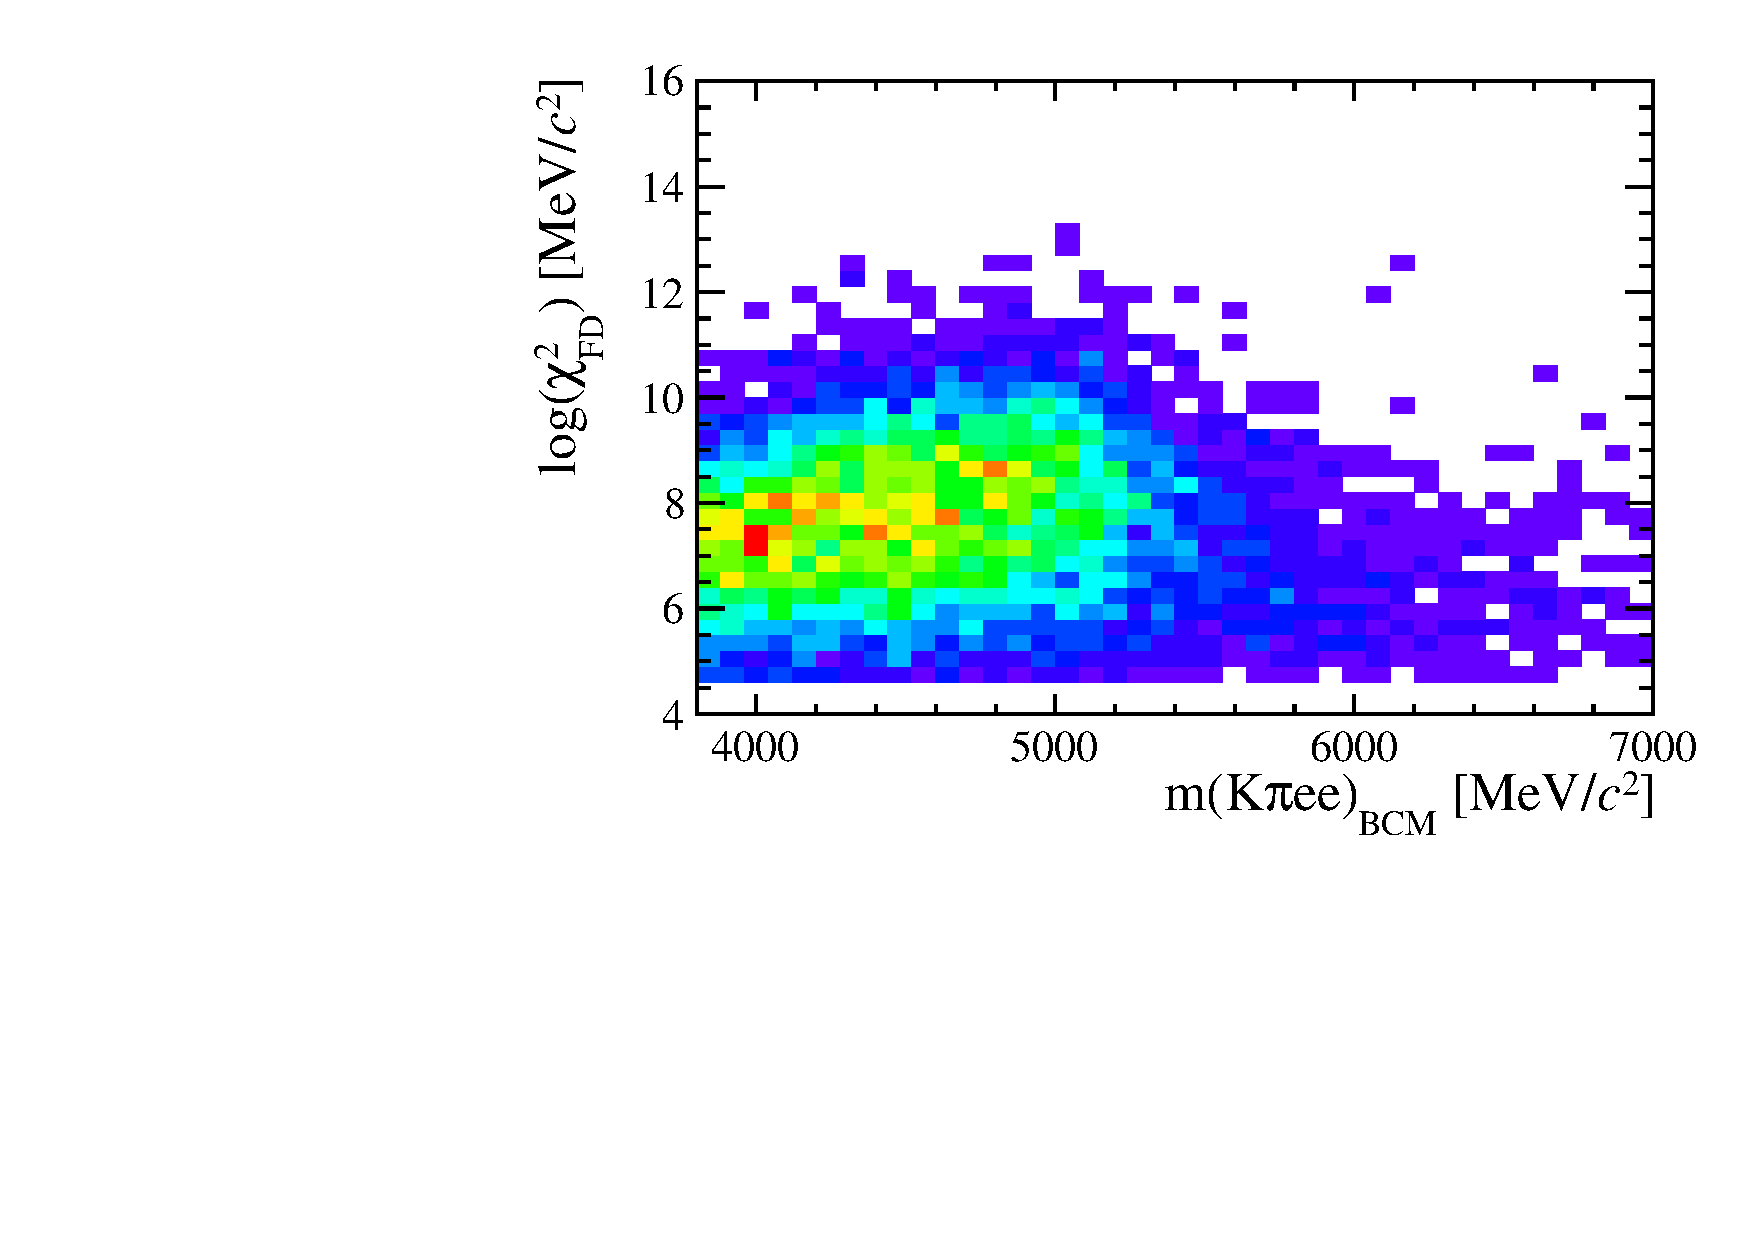
\includegraphics[width=0.48\textwidth]{RKst/figs/HOP/HOP_bkg_central.pdf}
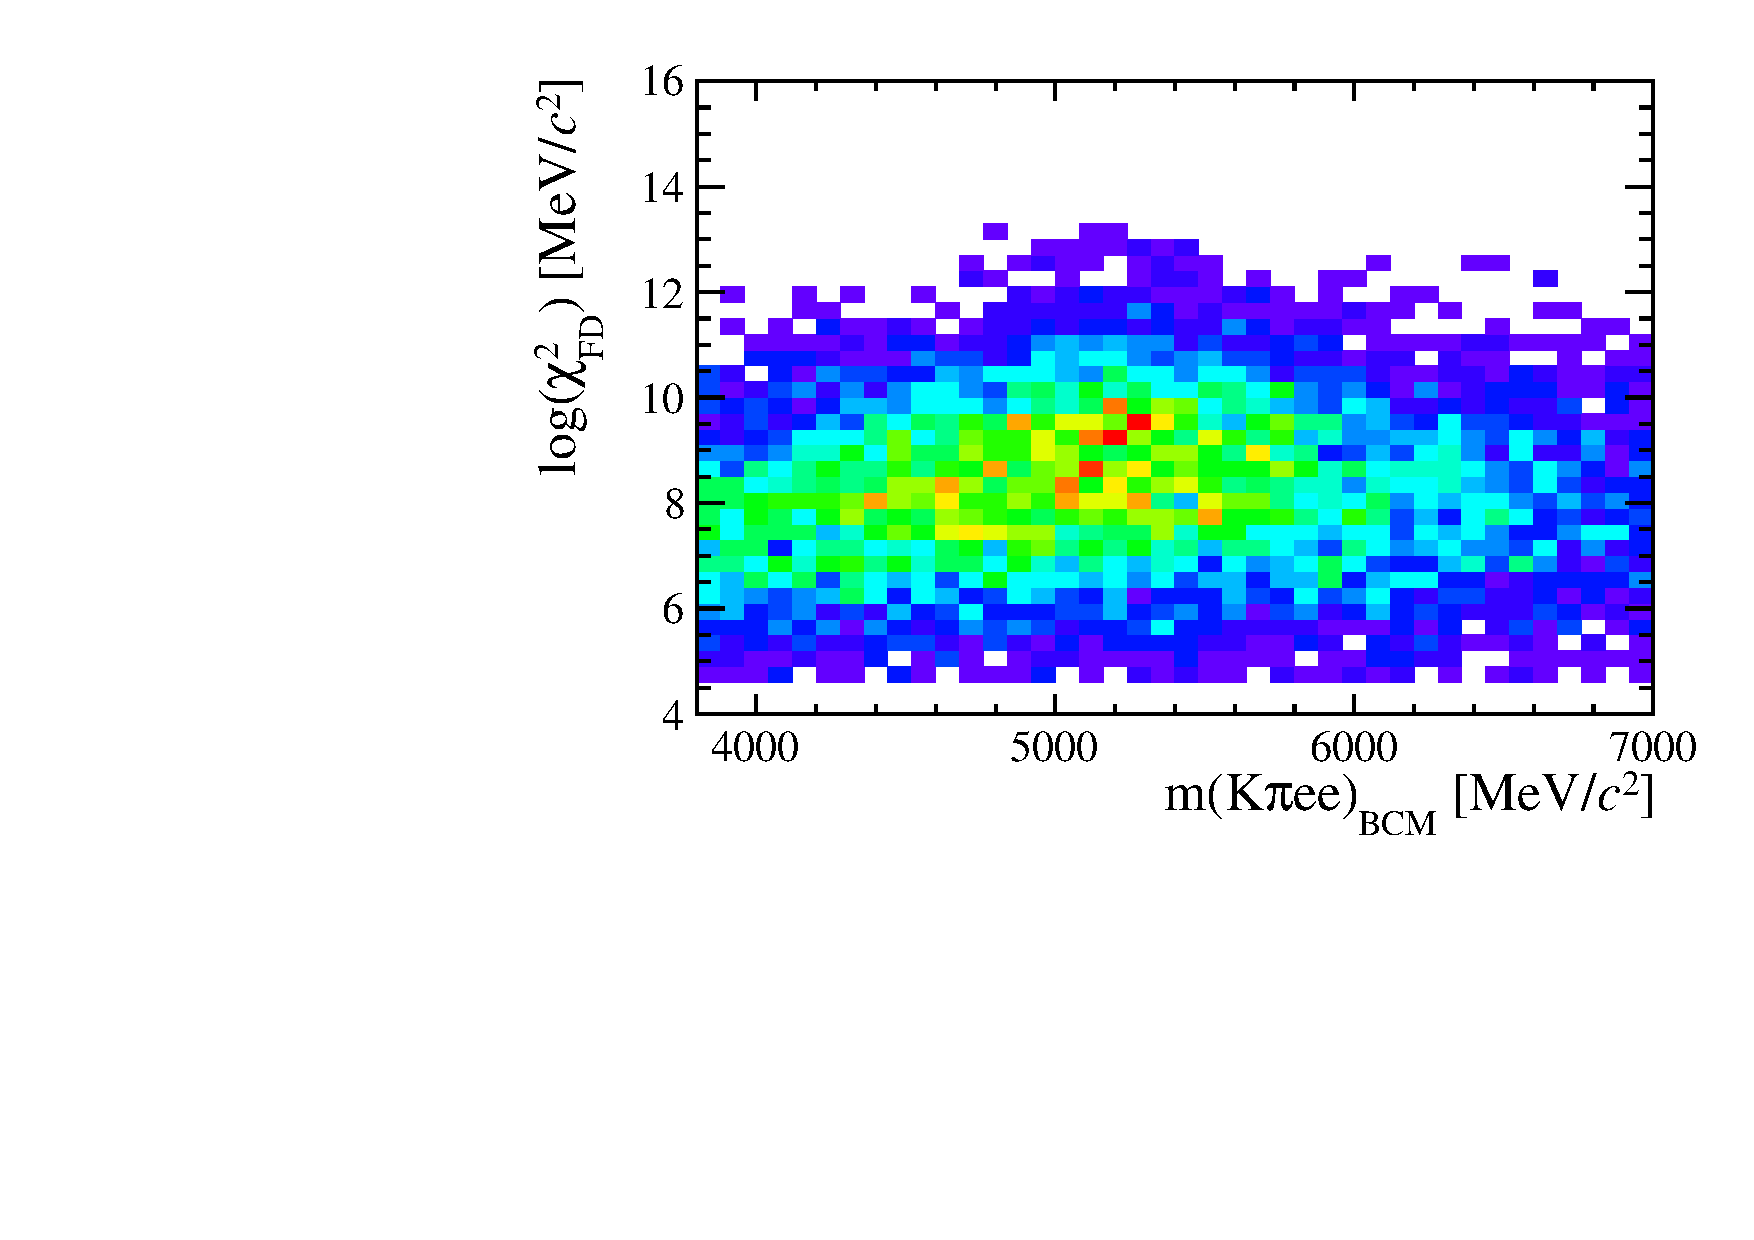
\includegraphics[width=0.48\textwidth]{RKst/figs/HOP/HOP_sig_high.pdf}
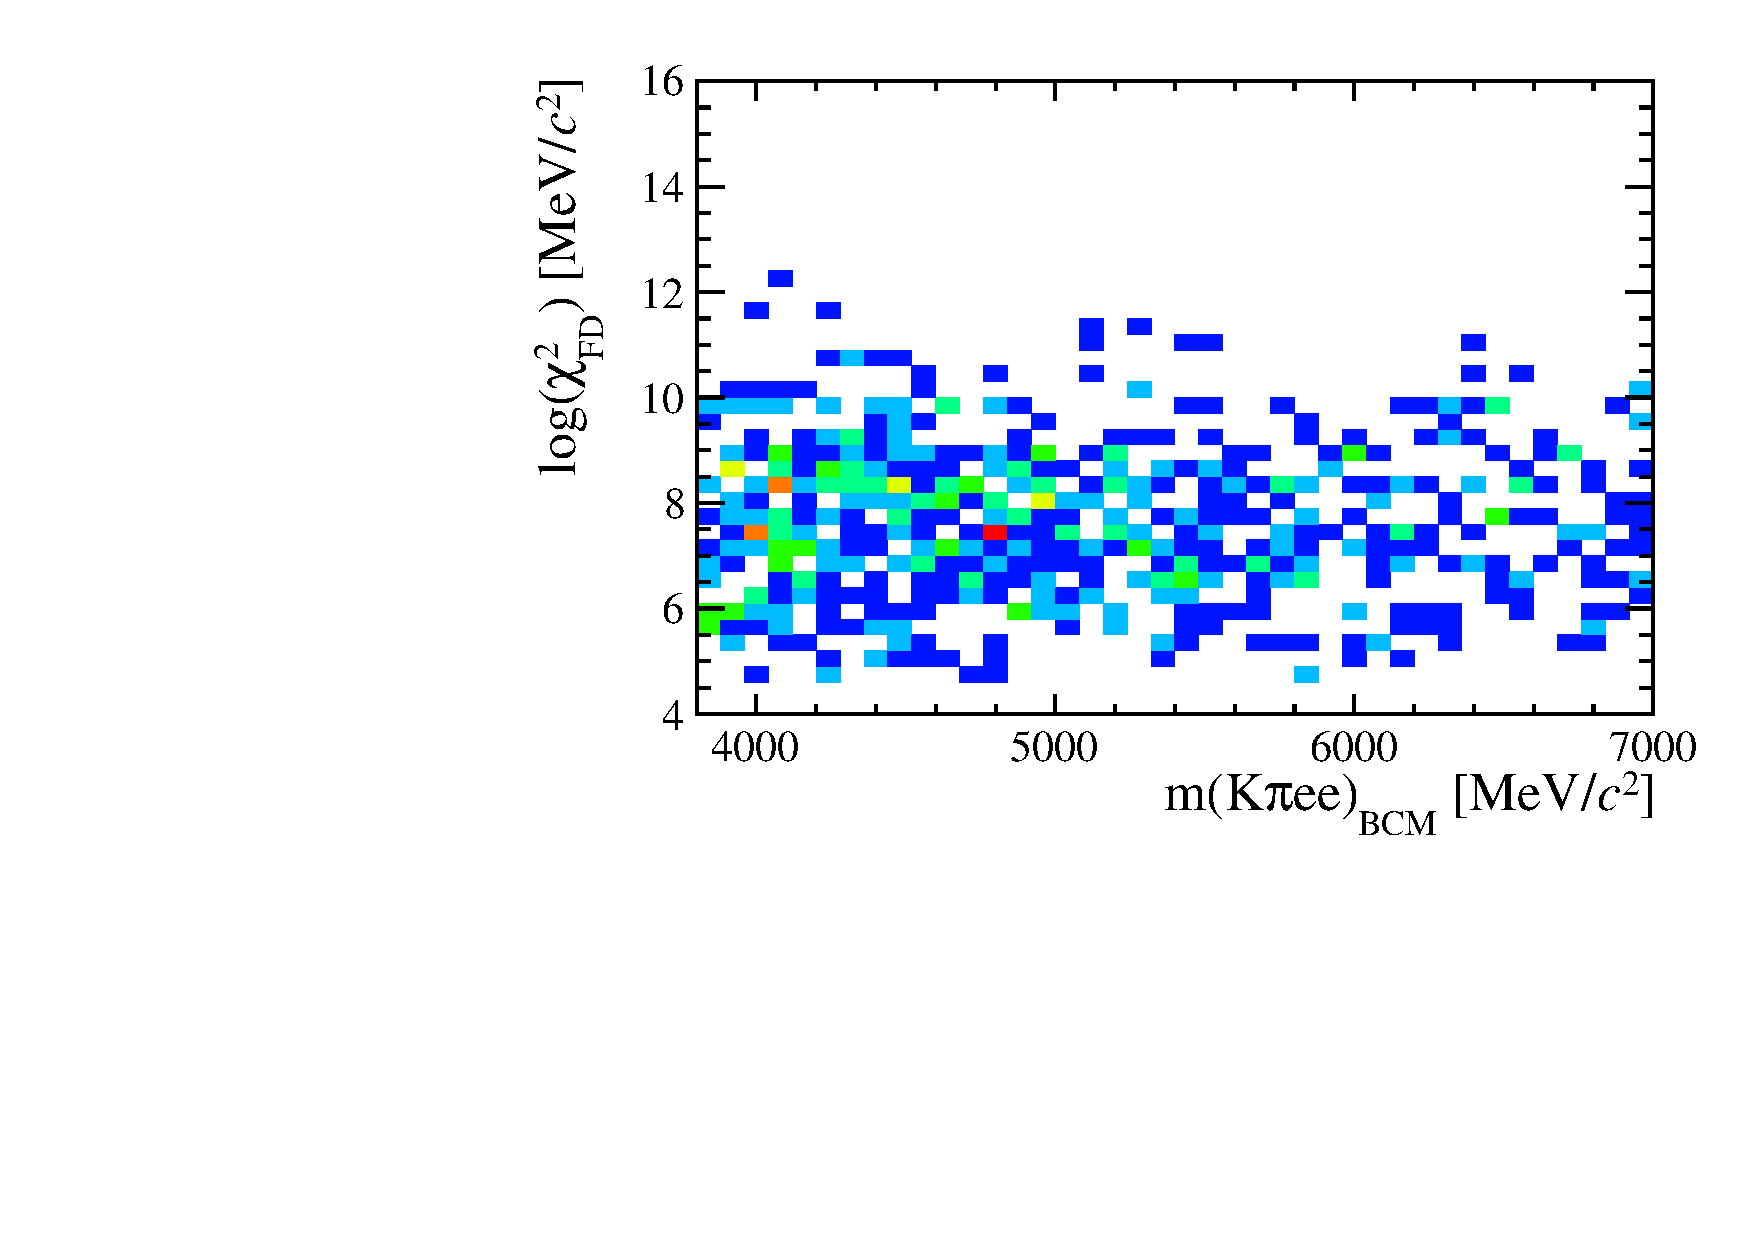
\includegraphics[width=0.48\textwidth]{RKst/figs/HOP/HOP_bkg_high.pdf}
\caption{Two-dimensional distribution of $\chi^2_{\rm FD}$ \vs \mbcm for (left) \BdToKstee signal and (right) partially-reconstructed background.
From top to bottom the low-, central- and high-\qsq intervals.}
\label{fig:hop}

%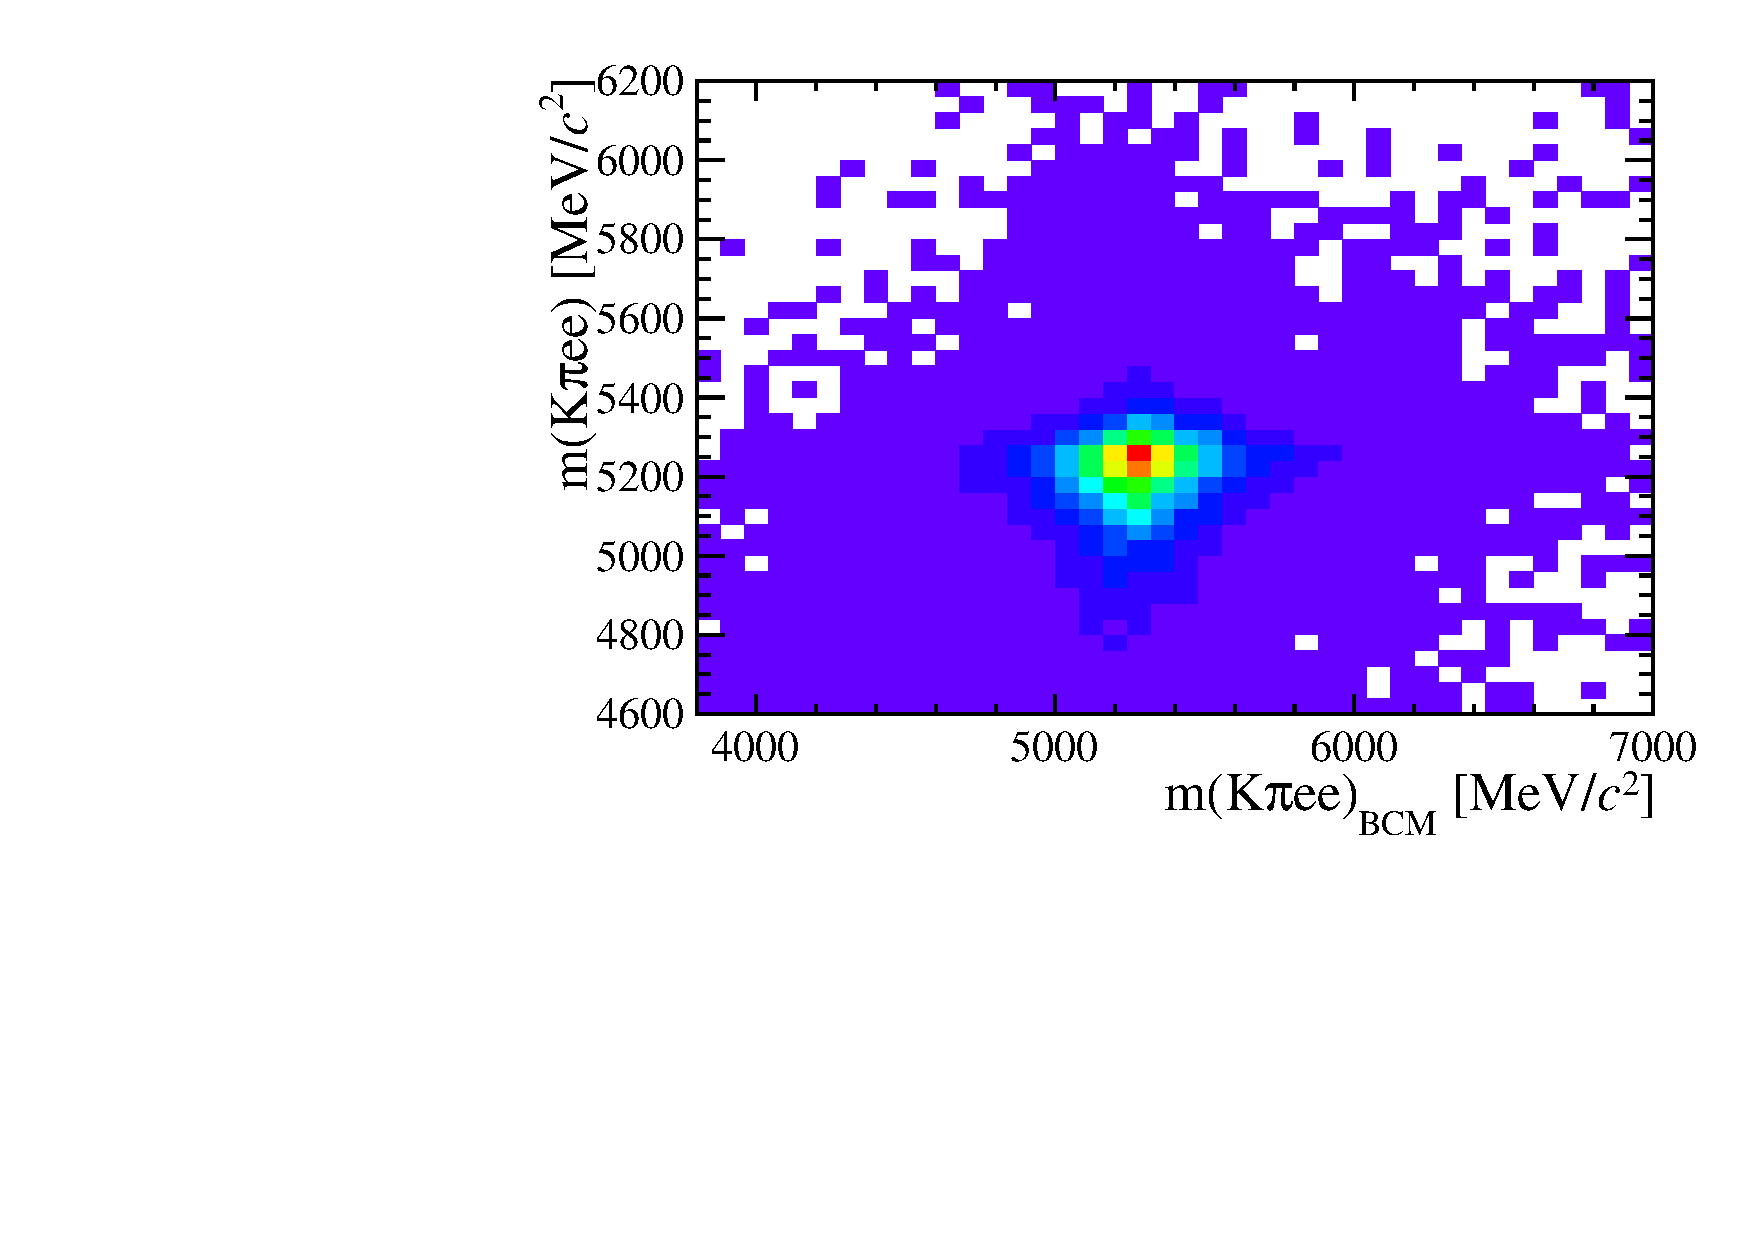
\includegraphics[width=0.48\textwidth]{RKst/figs/HOP/HOPvsM_sig_low.pdf}
%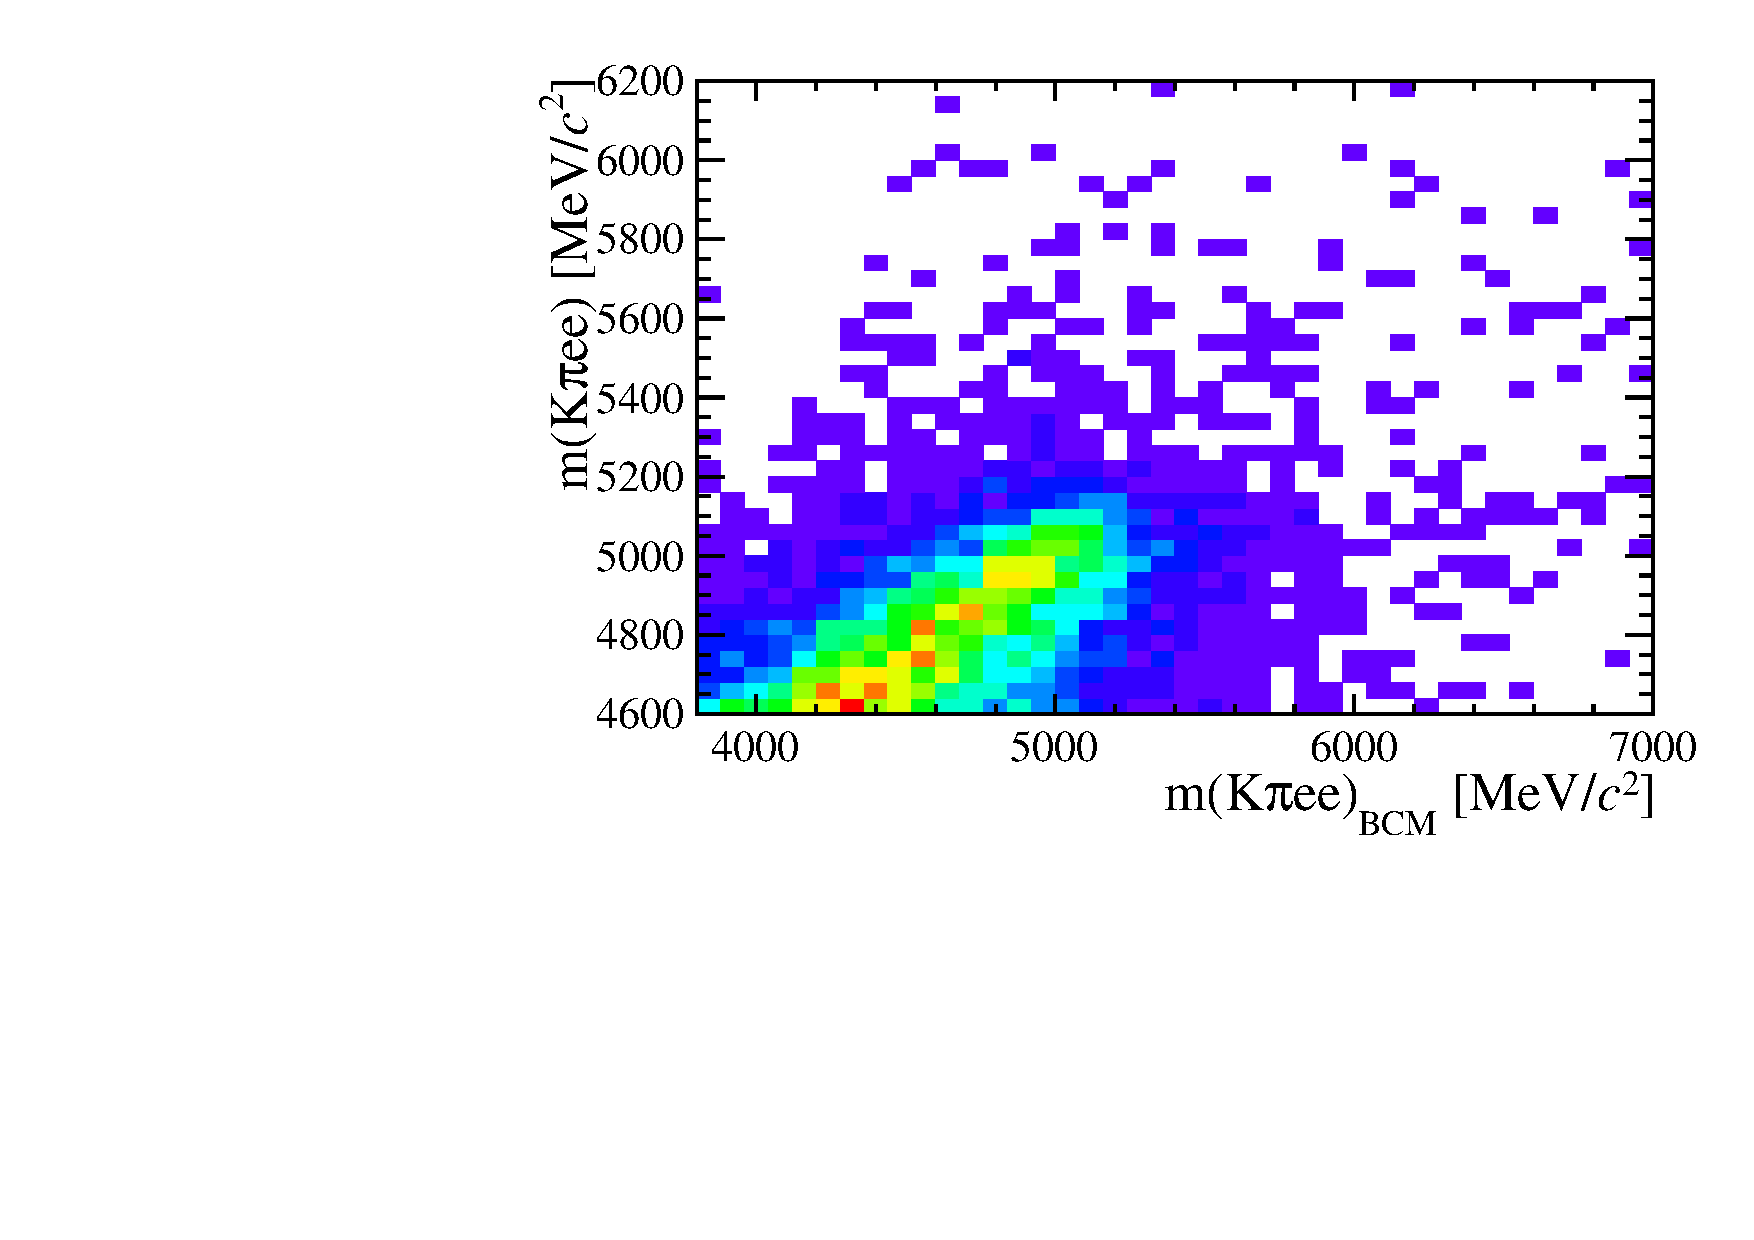
\includegraphics[width=0.48\textwidth]{RKst/figs/HOP/HOPvsM_bkg_low.pdf}
%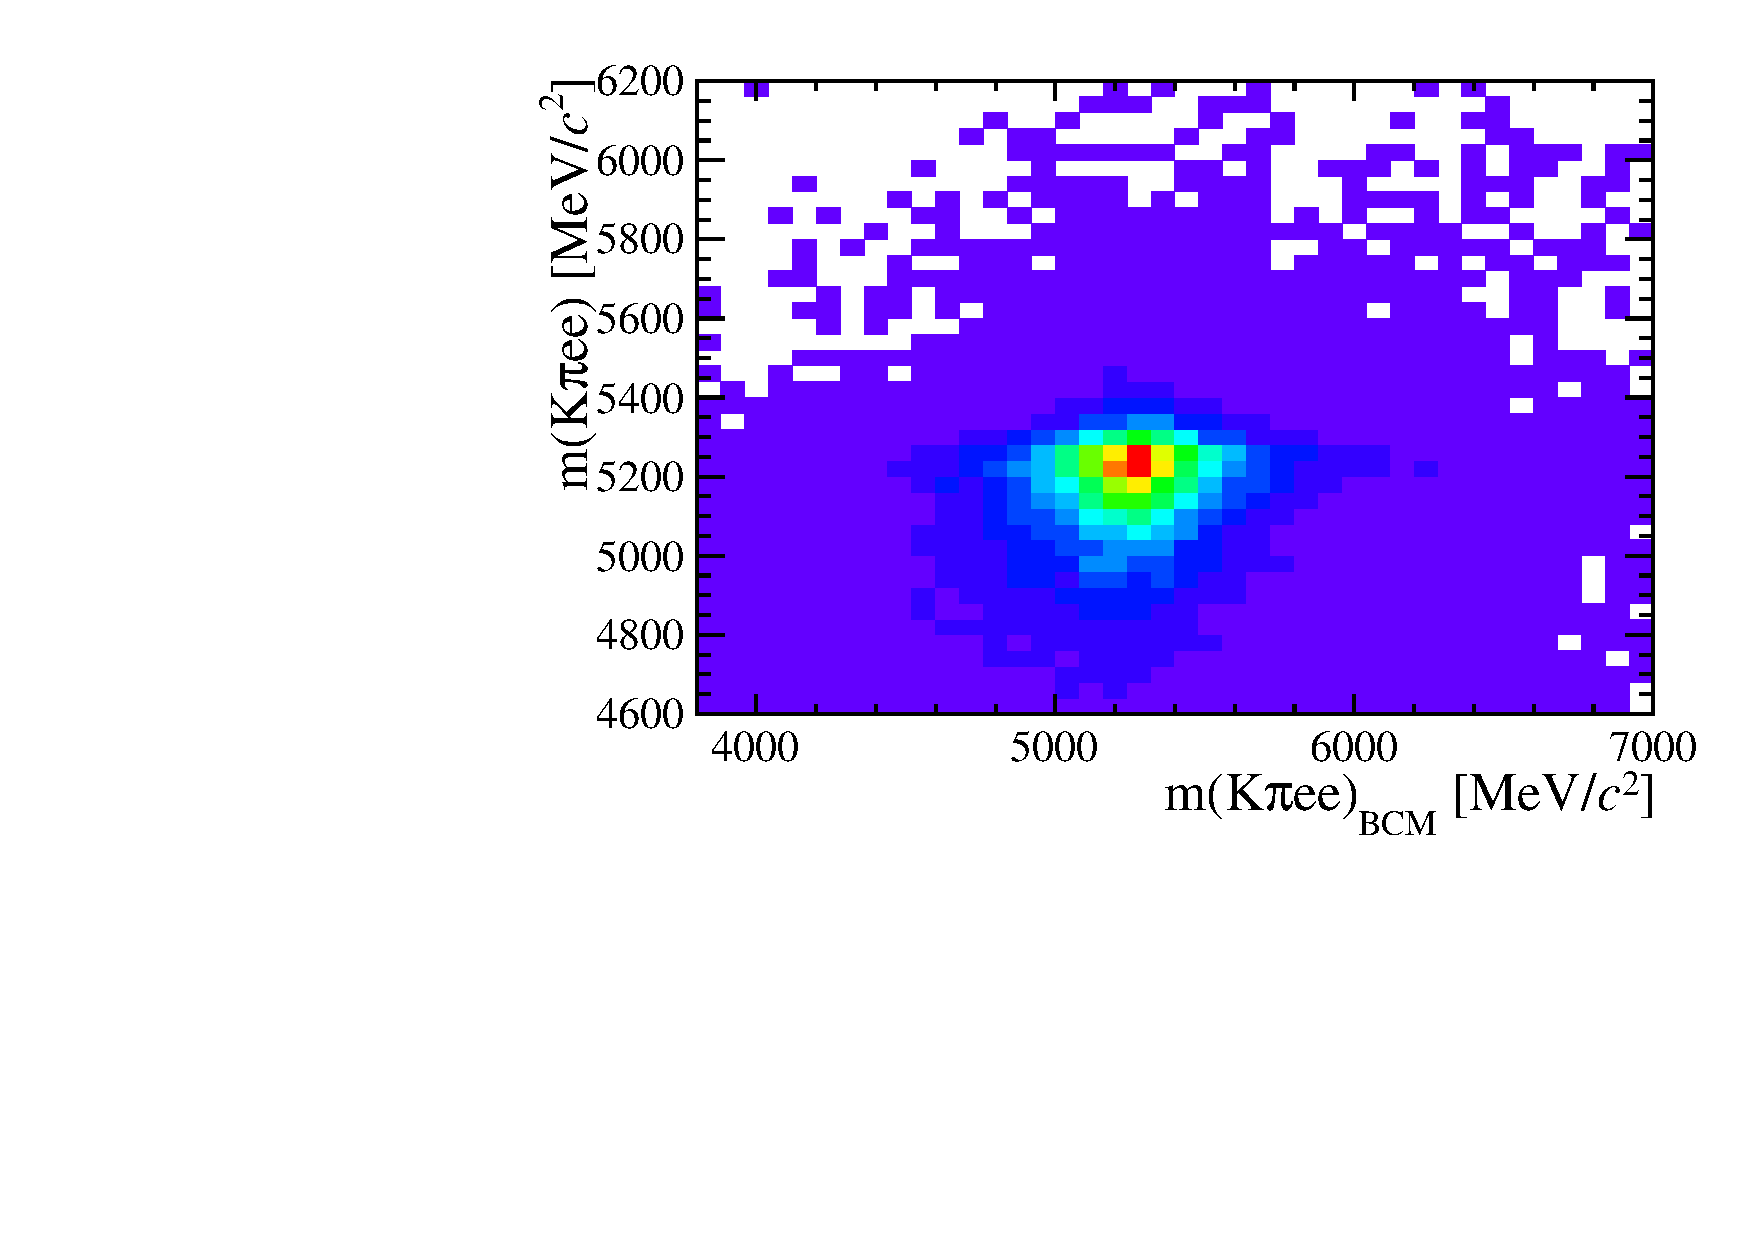
\includegraphics[width=0.48\textwidth]{RKst/figs/HOP/HOPvsM_sig_central.pdf}
%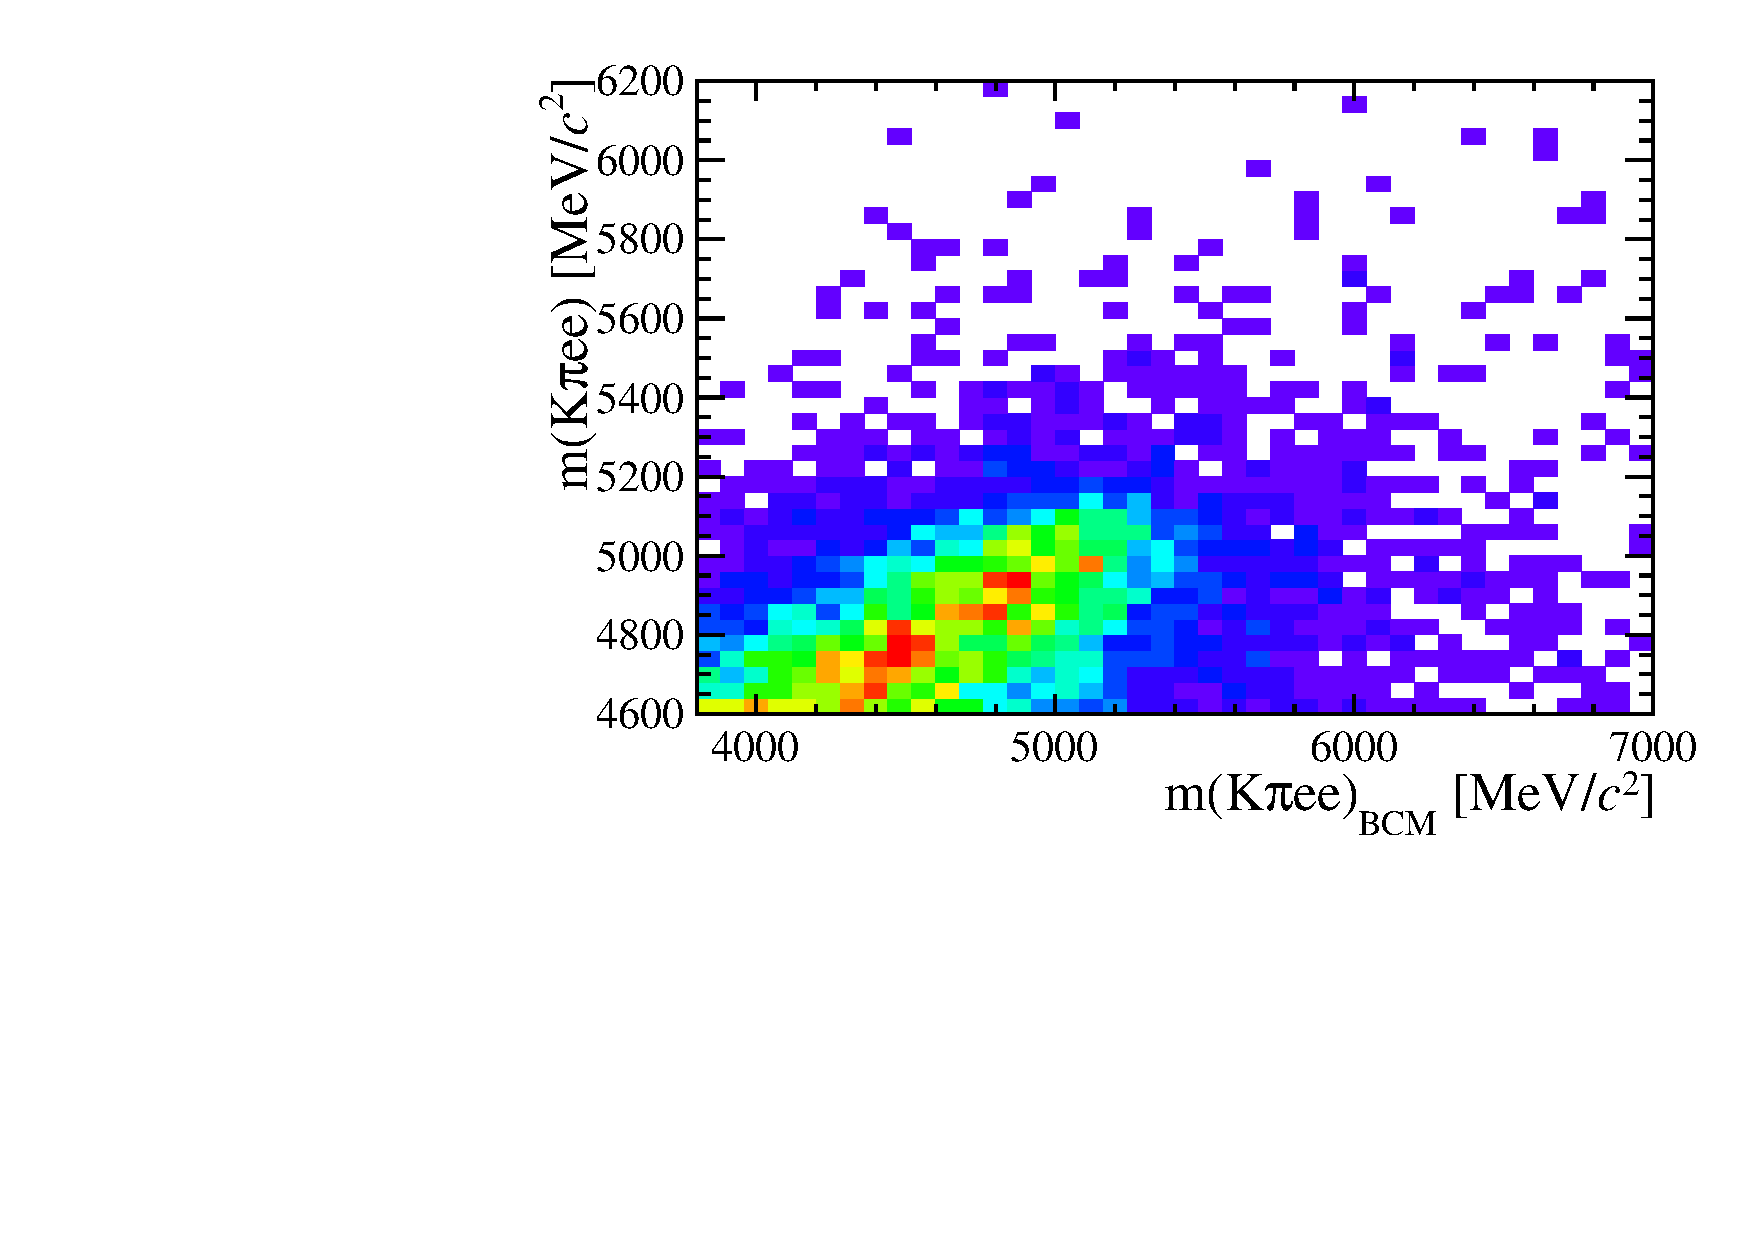
\includegraphics[width=0.48\textwidth]{RKst/figs/HOP/HOPvsM_bkg_central.pdf}
%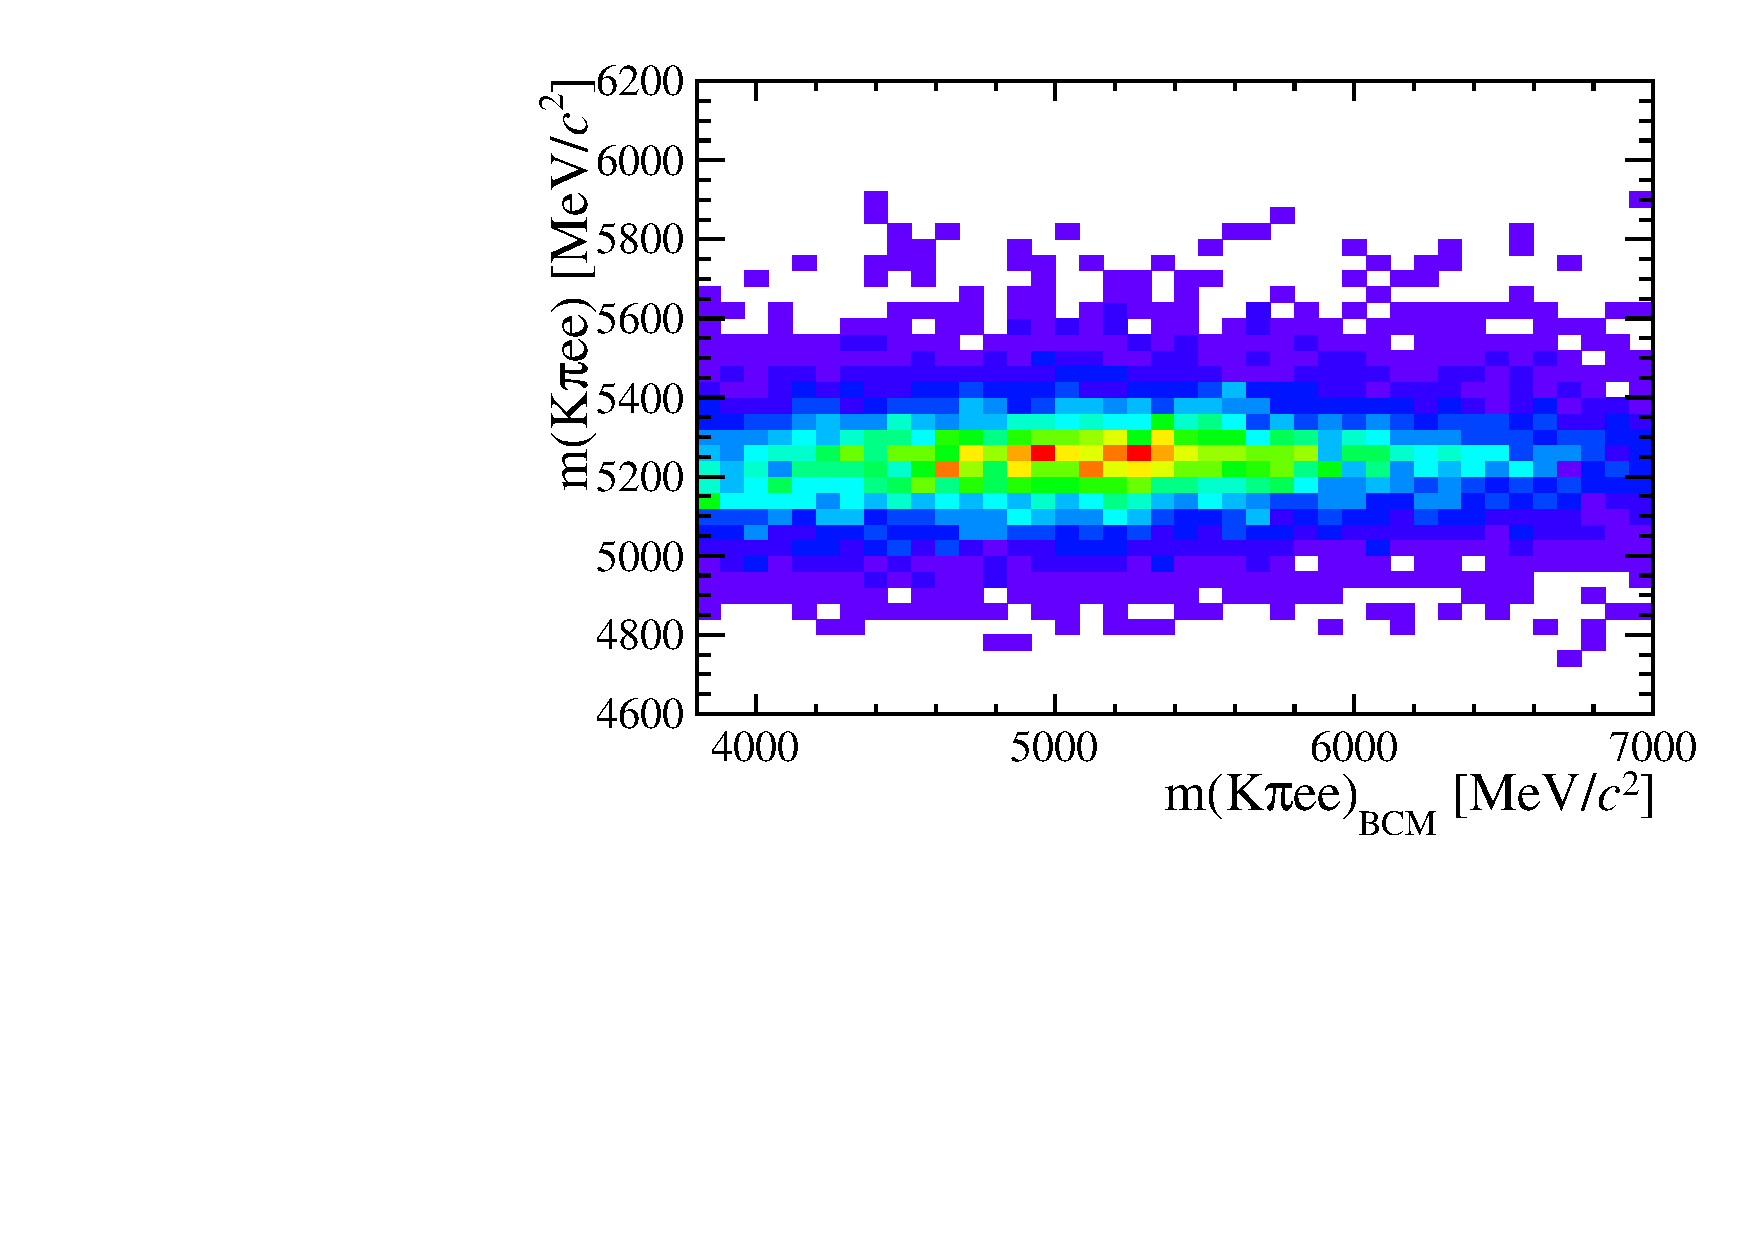
\includegraphics[width=0.48\textwidth]{RKst/figs/HOP/HOPvsM_sig_high.pdf}
%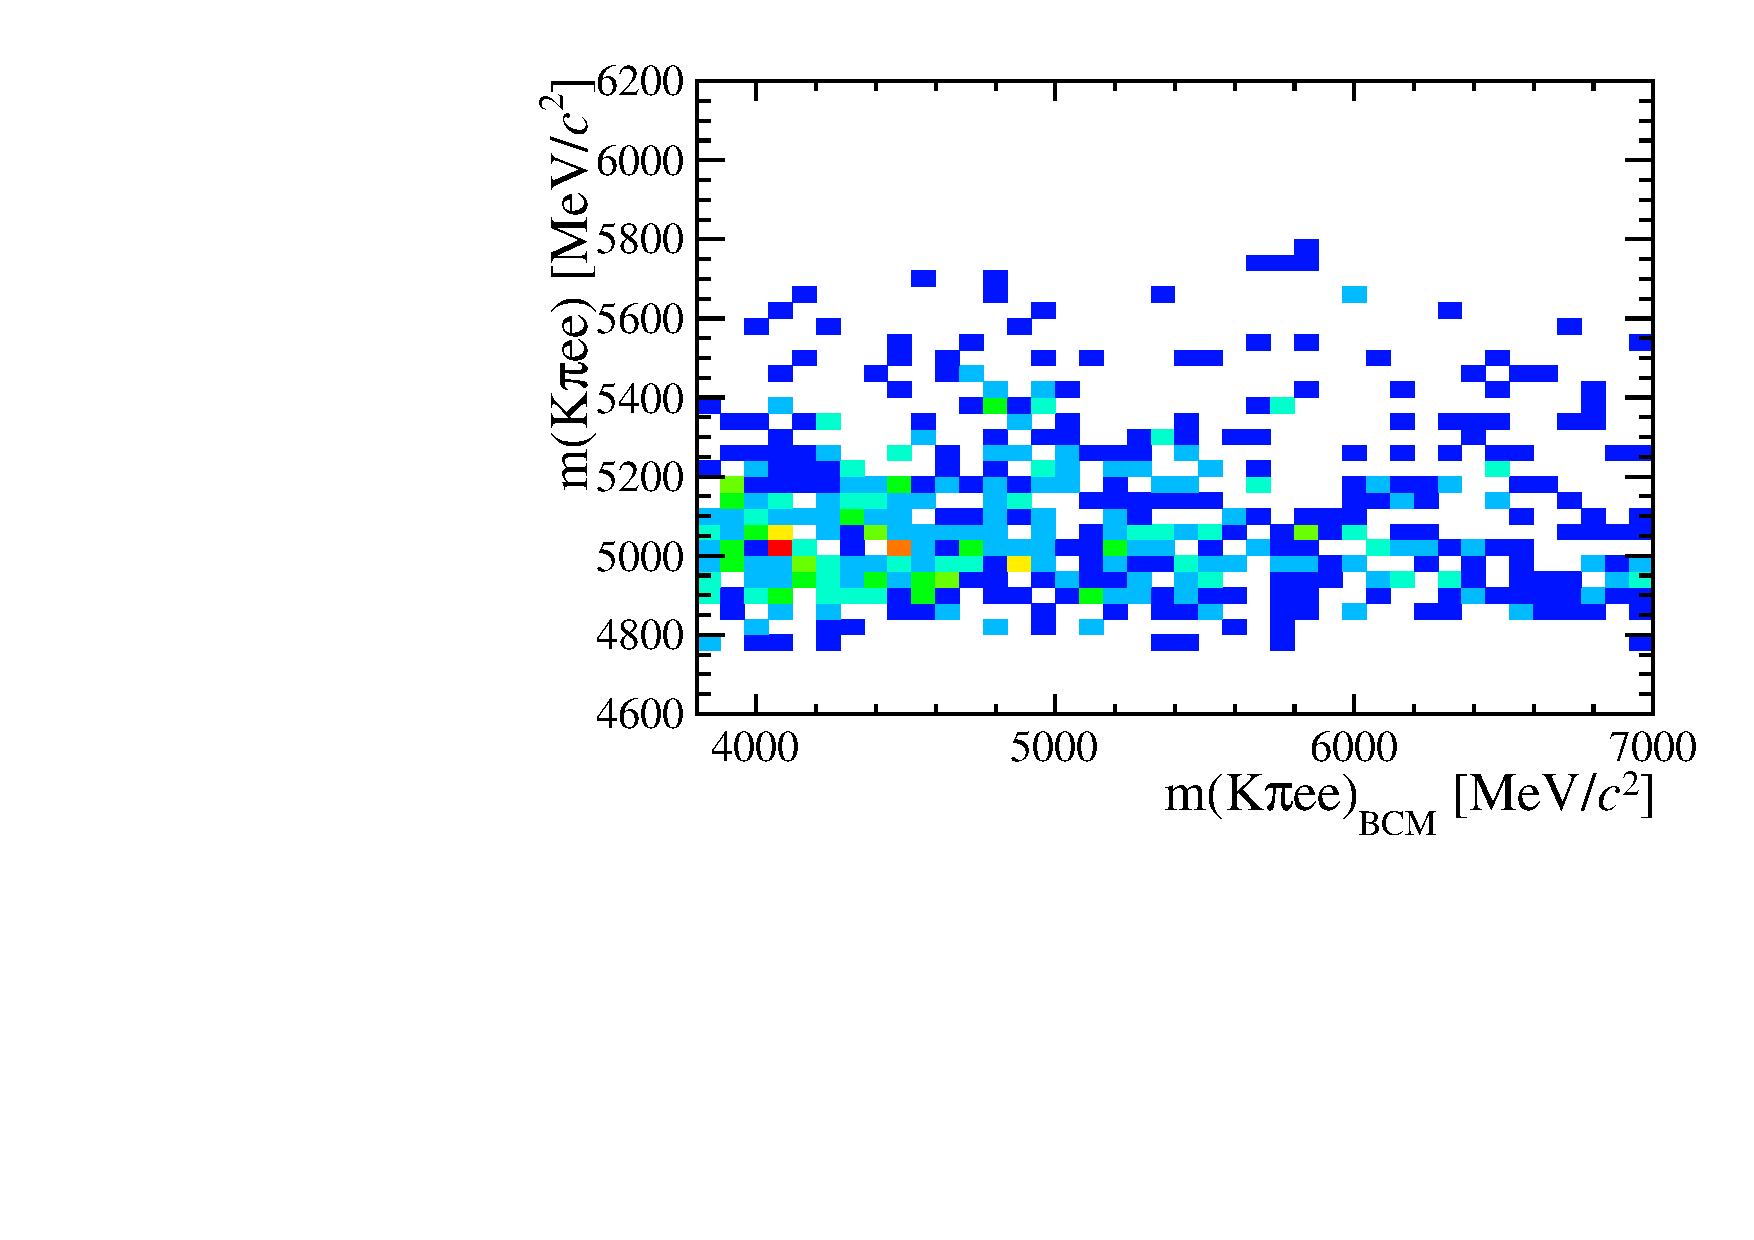
\includegraphics[width=0.48\textwidth]{RKst/figs/HOP/HOPvsM_bkg_high.pdf}
%\caption{Two-dimensional distribution of $m(K\pi ee) \vs \mbcm for (left) \BdToKstee signal and (right) partially-reconstructed background.
%From top to bottom the low-, central- and high-\qsq intervals.}
%\label{fig:hop2}
\end{figure}


\subsection{Multivariate analysis}
\label{sec:RKst_mva}

The final selection is performed using a neural network classifier based on the \mbox{\textsc{NeuroBayes}}
package~\cite{Feindt:2006pm,feindt-2004}. The multivariate analysis is intended to remove
some combinatorial background and obtain a clearer signal peak. In order to avoid biases, a so-called $k$-fold
approach is adopted to train and optimise the classifier, using $k=10$. In this method, the samples are divided into 
$k$ equally sized subsamples; $k$ classifiers are then trained and optimised each one using $(k-1)$ of the subsamples 
and applied to the $k$th one. This approach ensures that a classifier is never applied to the candidates used for its training.
Each classifier is trained on half of the candidates included in the $(k-1)$ samples and optimised using the other half,
which ensures that candidates used for training are not used for optimisation.

{\bf Samples:}

Representative samples of the signal and background are needed to train the classifier.
For the signal, fully reconstructed \BdToKstmm and \BdKstee simulated events can be used.
%The simulation is corrected improve the data-simulation agreement as described in (see Sec. \ref{sec:RKst_mc_weighting}).
Instead a sample representative of the background can be obtained using real data candidates
in the upper \Bz sideband: $m(K\pi\mu\mu) > 5400$~\mevcc~ and $m(K\pi ee) > 5600$~\mevcc.
The lower sideband is not used in the training as it contains a significant fraction of misreconstructed background.
All pre-selection requirements are applied to the background samples used for the training.
As L0 and PID variables are not well described in simulation these cuts are not applied to the simulation
but their effect is taken into account by event weights.
%To train the classifier 50\% of the sideband events was used, keeping the other 50\% for testing.
An approximately equal number of signal and background candidates is used for the training
which corresponds to about $10^3$ electron and $10^4$ muon candidates.
%, which
%is driven by the amount of background available.

{\bf Training:}

The neural network input consists of 24 variables carrying information about the kinematics of the decays
and the quality of tracks and vertices. All the variables used are listed in Tab.~\ref{tab:RKst_mva_vars}.
% and their correlation is graphically represented in Fig.~\ref{fig:Rkst_nnCorrelation}.
%In these figures the variable with ID = 1 is the neural-network output and the other IDs are reported in Tab.~\ref{tab:RKst_mva_vars}.
The single most discriminating variable is $\chisq_{\rm DTF}$, the \chisq of a kinematic fit (see Sec.~\ref{sec:DTF})
that constrains the decay product of the \Bz, the \Kstarz and the dimuon, to originate from their respective vertices.
Other variables that contribute significantly are the \chisqip of \jpsi and \Kstarz, the transverse momentum
of the \Bz and the pointing direction (\verb!DIRA!) of the reconstructed \Bz to the primary vertex.
%
%
\begin{table}
\centering
\caption{List of variables used as inputs for the neural-network training.
%Next to each variable the ID number in brackets provides the index
%reported in the correlation matrices shown in Fig.~\ref{fig:Rkst_nnCorrelation}.
}
\begin{tabular}{$l|^l}
\rowstyle{\bfseries}
Particle 	& Variables \\ \hline
\Bz		& \pt, \quad \chisqip, \quad $\chisq_{\rm FD}$, \quad $\chisq_{vtx}/\text{ndf}$, \quad \texttt{DIRA}, \quad $\chisq_{\rm DTF}/\text{ndf}$ \\
\Kstarz	& \pt, \quad \chisqip, \quad $\chisq_{\rm FD}$, \quad $\chisq_{vtx}/\text{ndf}$, \quad \texttt{DIRA} \\
$h$		& $\mathrm{min},\mathrm{max}(p_{\textrm{T}, \kaon},p_{\textrm{T}, \pi})$, \quad $\mathrm{min},\mathrm{max}(\chi_{\textrm{IP}, \kaon}^{2},\chi_{\textrm{IP}, \pi}^{2})$ \\
$\ell\ell$	& \pt, \quad \chisqip, \quad $\chisq_{\rm FD}$, \quad $\chisq_{vtx}/\text{ndf}$, \quad \texttt{DIRA} \\
$\ell$	& $\mathrm{min},\mathrm{max}(p_{\textrm{T}, \ell^+},p_{\textrm{T}, \ell^-})$, \quad $\mathrm{min},\mathrm{max}(\chi_{\textrm{IP}, \ell^+}^{2},\chi_{\textrm{IP}, \ell^-}^{2})$ \\
%\Bz			& $\chi^2_{\rm DTF}/\text{ndf}$ [1], DIRA [19], $\chi^2_{\rm FD}$ [15], $\chi^2_{vtx}/\text{ndf}$ [12], \chisqip [14], \pt [7] \\
%\Kstar		& $\chi^2_{\rm FD}$ [21], $\chi^2_{vtx}/\text{ndf}$ [11], \chisqip [2], \pt [5] \\
%Dilepton	& $\chi^2_{\rm FD}$ [17], $\chi^2_{vtx}/\text{ndf}$ [13], \chisqip [20], \pt [6] \\
%$e$			& \chisqip [3][4], \pt [9][10]\\
%$\mu$		& \chisqip [14][15], \pt [9][10]\\
%K			& \chisqip [18], \pt [16]\\
%$\pi$		& \chisqip [22], \pt [8]\\
\end{tabular}
\label{tab:RKst_mva_vars}
\end{table}
%
\begin{figure}[b]
\centering
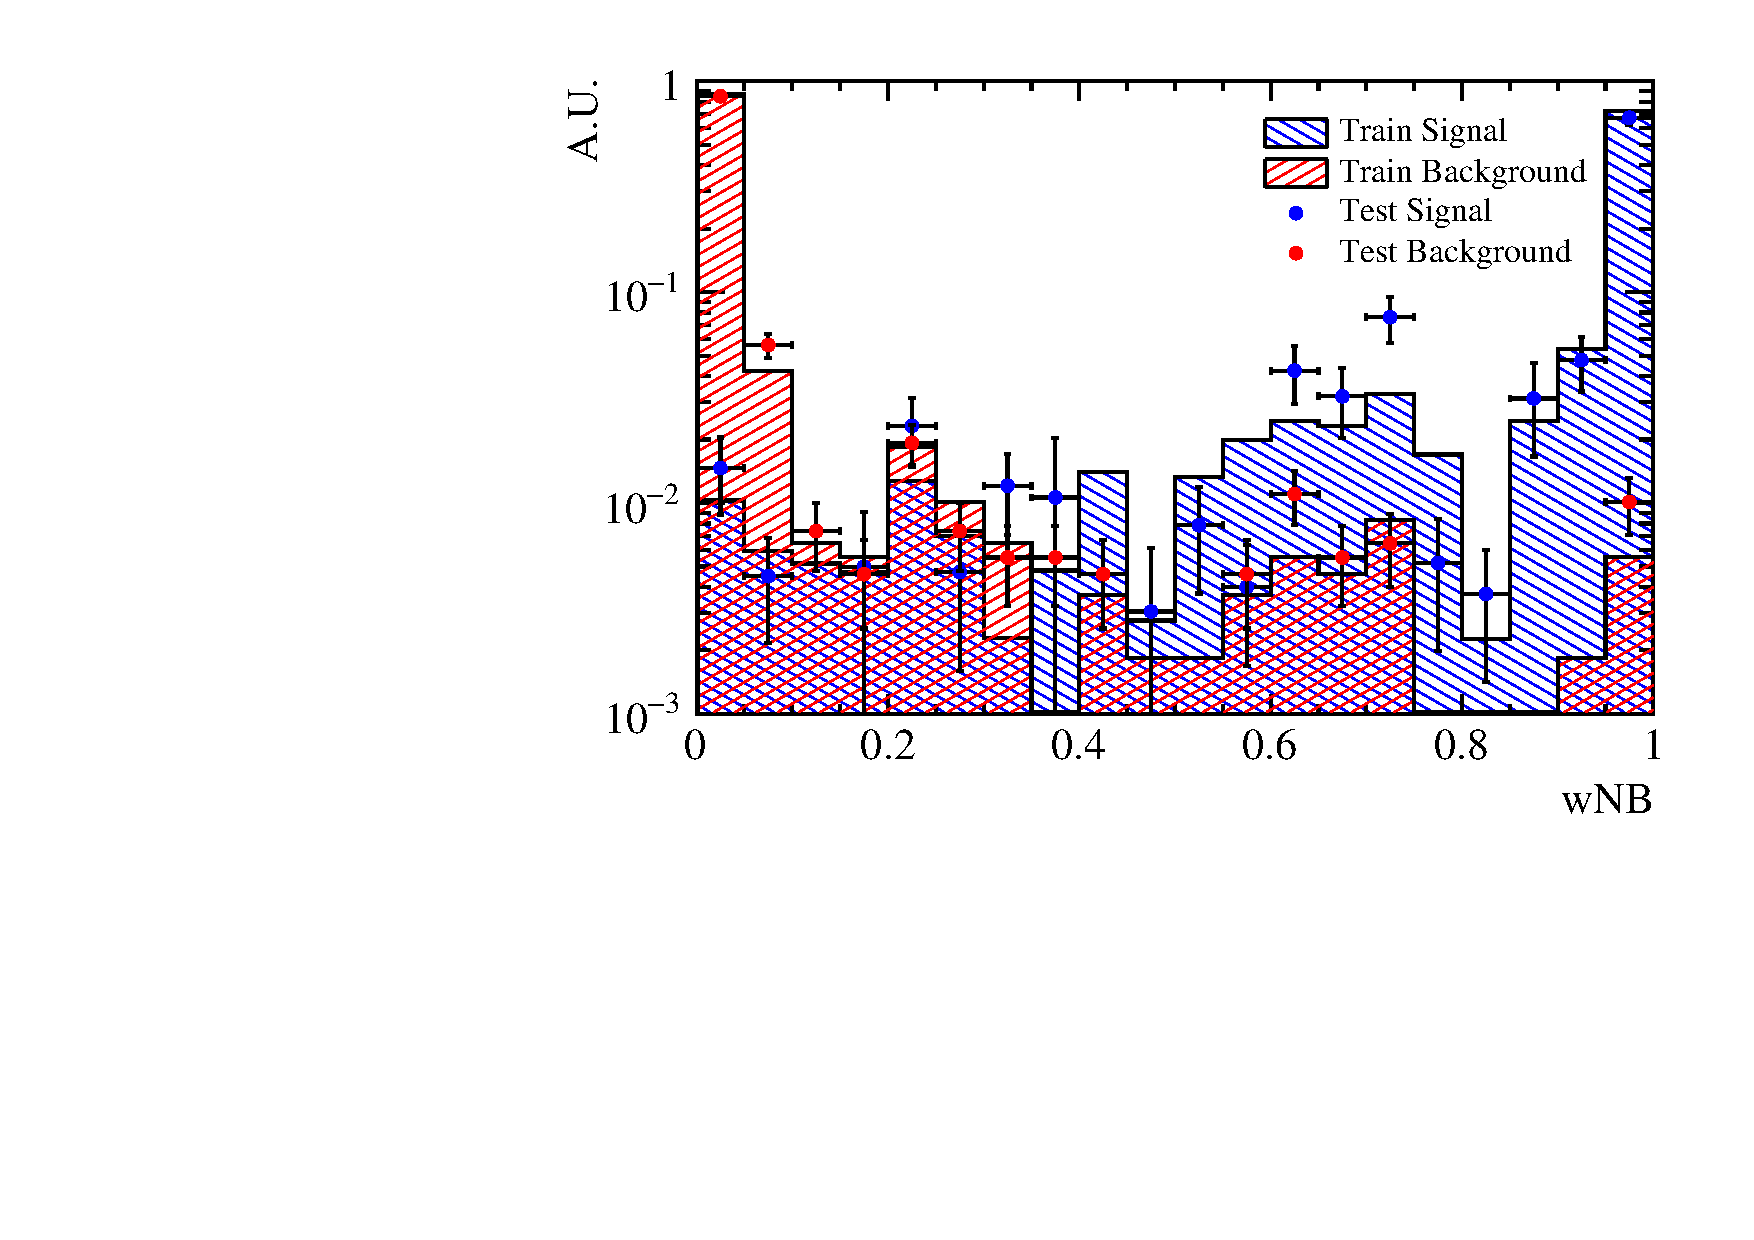
\includegraphics[width=0.49\textwidth]{RKst/figs/Training/EE_wNB_TrainAndTest.pdf}
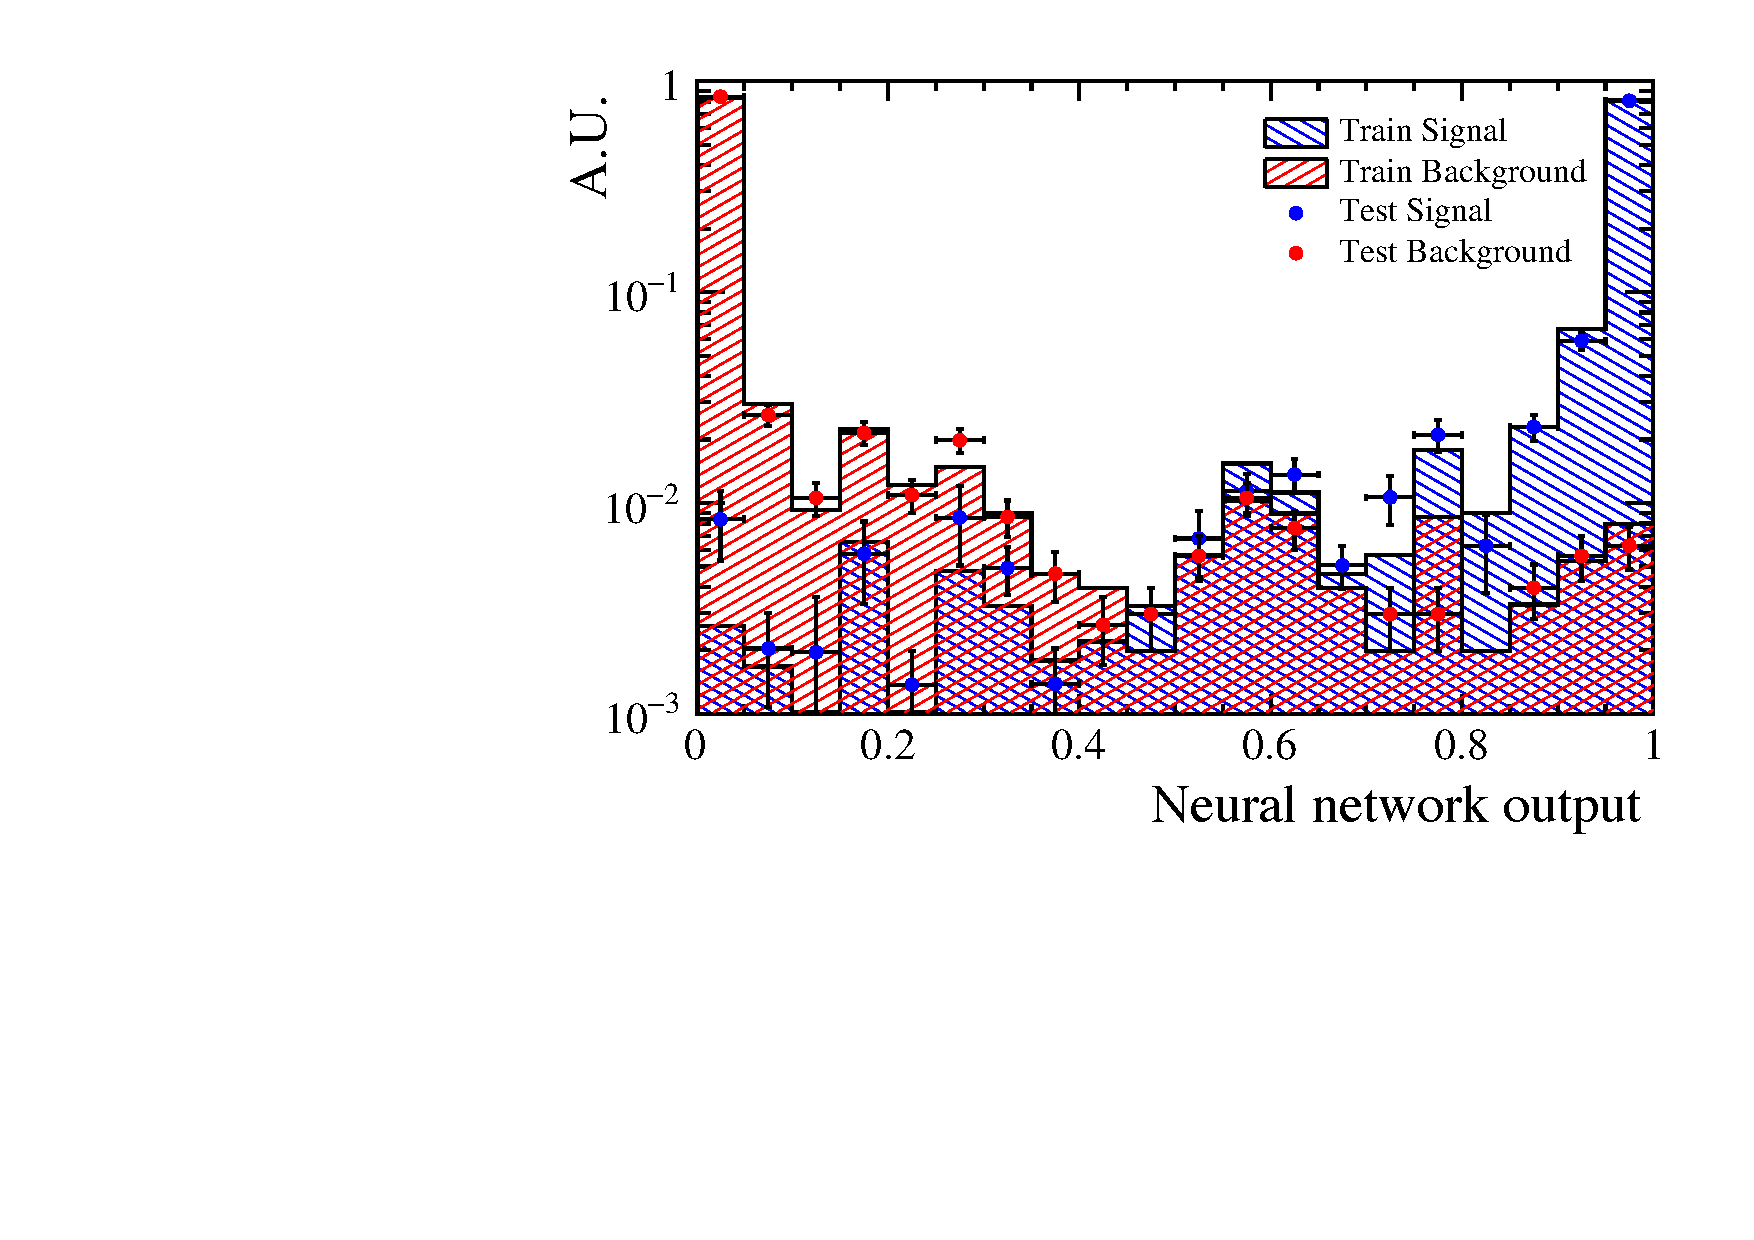
\includegraphics[width=0.49\textwidth]{RKst/figs/Training/MM_wNB_TrainAndTest.pdf}
\caption{Neural network output distributions for training (solid) and test (stripes) samples, for simulated 
signal (blue) and data sideband (red) candidates. For the electron (left) and muon (right) training.}
\label{fig:RKst_nnDist}
\end{figure}
%
%The list the 5 most important variables is reported in Tab.~\ref{tab:RKst_nnInputs}, together
%with information on the relative importance of each input. The meaning of the column headings
%in this table was already explained in Sec.~\ref{sec:Lb_mva}.

%\begin{table}
%\centering
%\caption{Summary of inputs to the neural network in order of importance. The 5 most discriminating variables are shown.
%Column ``adds'' gives correlation significance added by given input when adding it to list of those
%ranked above, ``only this'' provides power of given input alone and ``loss'' shows how much information
%is lost when removing only given input. Decay Tree Fit is performed using DecayTreeFitter tool
%on whole decay chain with constraining tracks to appropriate vertex topology and the $m(p\pi)$
%invariant mass to the PDG value.}
%\begin{tabular}{c|ccc|c|ccc}
%\multicolumn{4}{c|}{Muons} 														& \multicolumn{4}{c}{Electrons}				%		  \\ \hline   
%Input                   			& Adds 			& Only this 	& Loss 			& Input        							& Adds      & Only this & Loss    \\ \hline
%$ \Bz$ $\chi^2_{\rm DTF}/\text{ndf} $		& 80.44 		& 80.44 		& 13.14  		&	$ \Bz$ $\chi^2_{\rm DTF}/\text{ndf} $		& 28.70 		& 28.70 		& 3.94  \\
%$ \Kstar$ $\chisqip $		& 22.26 		& 67.58 		& 3.48  		&	$ \Kstar$ $\chisqip $		& 12.71 		& 25.11 		& 1.57  \\
%$ \Bz\text{DIRA} $		& 10.58 		& 71.24 		& 3.95  		&	$ e_{2}$ $\chisqip $		& 6.56 		& 20.19 		& 3.30  \\
%$ \Kstar$ $\pt $		& 9.16 		& 49.13 		& 2.07  		&	$ e_{1}$ $\chisqip $		& 5.54 		& 19.66 		& 2.60  \\
%$ \jpsi$ $\chisqip $		& 6.58 		& 56.15 		& 1.35  		&	$ \Kstar$ $\pt $		& 3.74 		& 15.35 		& 3.14  \\
%$ \Bz$ $\pt $		& 6.00 		& 41.42 		& 4.39  		&	$ \jpsi$ $\pt $		& 4.81 		& 5.55 		& 3.18  \\
%$ \mu_{1}$ $\pt $		& 2.96 		& 15.85 		& 3.79  		&	$ \Bz$ $\pt $		& 2.78 		& 13.01 		& 2.20  \\
%$ \mu_{2}$ $\pt $		& 2.73 		& 15.04 		& 3.46  		&	$ \pi$ $\pt $		& 3.08 		& 7.93 		& 1.83  \\
%$ \jpsi$ $\pt $		& 3.06 		& 16.41 		& 2.84  		&	$ e_{2}$ $\pt $		& 2.35 		& 9.81 		& 2.74  \\
%$ \Kstar$ $\chi^2_{vtx}/\text{ndf} $		& 2.41 		& 28.14 		& 2.38  		&	$ e_{1}$ $\pt $		& 2.15 		& 8.04 		& 2.28  \\

%$ \Bz$ $\chi^2_{\rm FD} $		& 2.03 		& 63.73 		& 1.37  		&	$ \Kstar$ $\chi^2_{vtx}/\text{ndf} $		& 1.75 		& 7.45 		& 1.89  \\
%$ \mu_{1}$ $\chisqip $		& 1.45 		& 47.90 		& 1.75  		&	$ \Bz$ $\chi^2_{vtx}/\text{ndf} $		& 1.83 		& 27.54 		& 1.95  \\
%$ \mu_{2}$ $\chisqip $		& 1.04 		& 43.24 		& 1.20  		&	$ \jpsi$ $\chi^2_{vtx}/\text{ndf} $		& 1.10 		& 11.28 		& 1.16  \\
%$ K$ $\chisqip $		& 0.84 		& 62.99 		& 0.71  		&	$ \Bz$ $\chisqip $		& 1.11 		& 14.35 		& 1.24  \\
%$ \jpsi$ $\chi^2_{\rm FD} $		& 0.60 		& 55.41 		& 0.62  		&	$ \Bz$ $\chi^2_{\rm FD} $		& 0.93 		& 25.65 		& 1.21  \\
%$ \Bz$ $\chi^2_{vtx}/\text{ndf} $		& 0.56 		& 74.60 		& 0.61  		&	$ K$ $\pt $		& 0.82 		& 14.26 		& 0.61  \\
%$ \pi$ $\pt $		& 0.55 		& 34.94 		& 0.48  		&	$ \jpsi$ $\chi^2_{\rm FD} $		& 0.69 		& 23.85 		& 0.63  \\
%$ \Kstar$ $\chi^2_{\rm FD} $		& 0.34 		& 64.88 		& 0.41  		&	$ K$ $\chisqip $		& 0.56 		& 23.59 		& 0.52  \\
%$ \pi$ $\chisqip $		& 0.32 		& 56.92 		& 0.30  		&	$ \Bz\text{ $		& 0.53 		& 24.50 		& 0.52  \\
%$ \Bz$ $\chisqip $		& 0.30 		& 52.17 		& 0.30  		&	$ \jpsi$ $\chisqip $		& 0.37 		& 23.54 		& 0.38  \\
%$ \jpsi$ $\chi^2_{vtx}/\text{ndf} $		& 0.07 		& 18.35 		& 0.07  		&	$ \Kstar$ $\chi^2_{\rm FD} $		& 0.09 		& 23.66 		& 0.07  \\
%$ K$ $\pt $		& 0.03 		& 43.58 		& 0.03  		&	$ \pi$ $\chisqip $		& 0.01 		& 19.89 		& 0.01  \\
%\end{tabular}
%\label{tab:RKst_nnInputs}
%\end{table}

%\begin{figure}
%\centering
%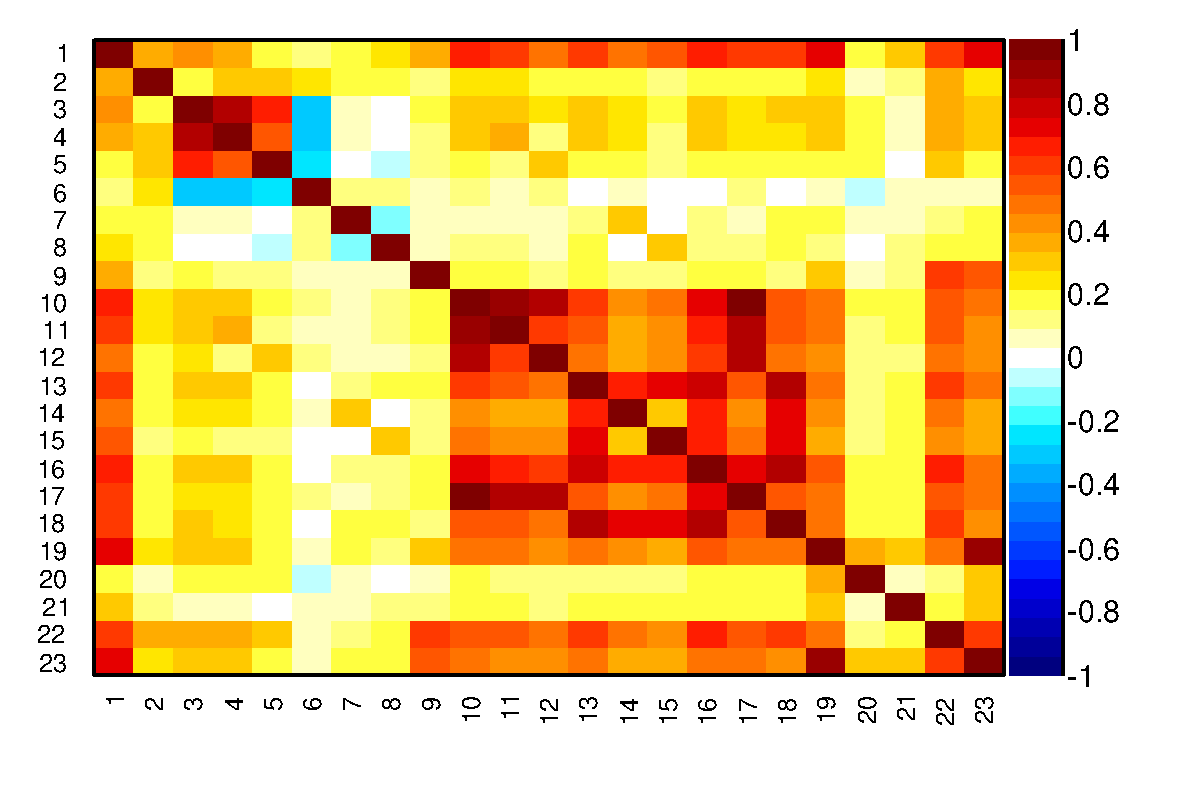
\includegraphics[width=0.8\textwidth]{RKst/figs/Training/electrons/correlation.pdf}
%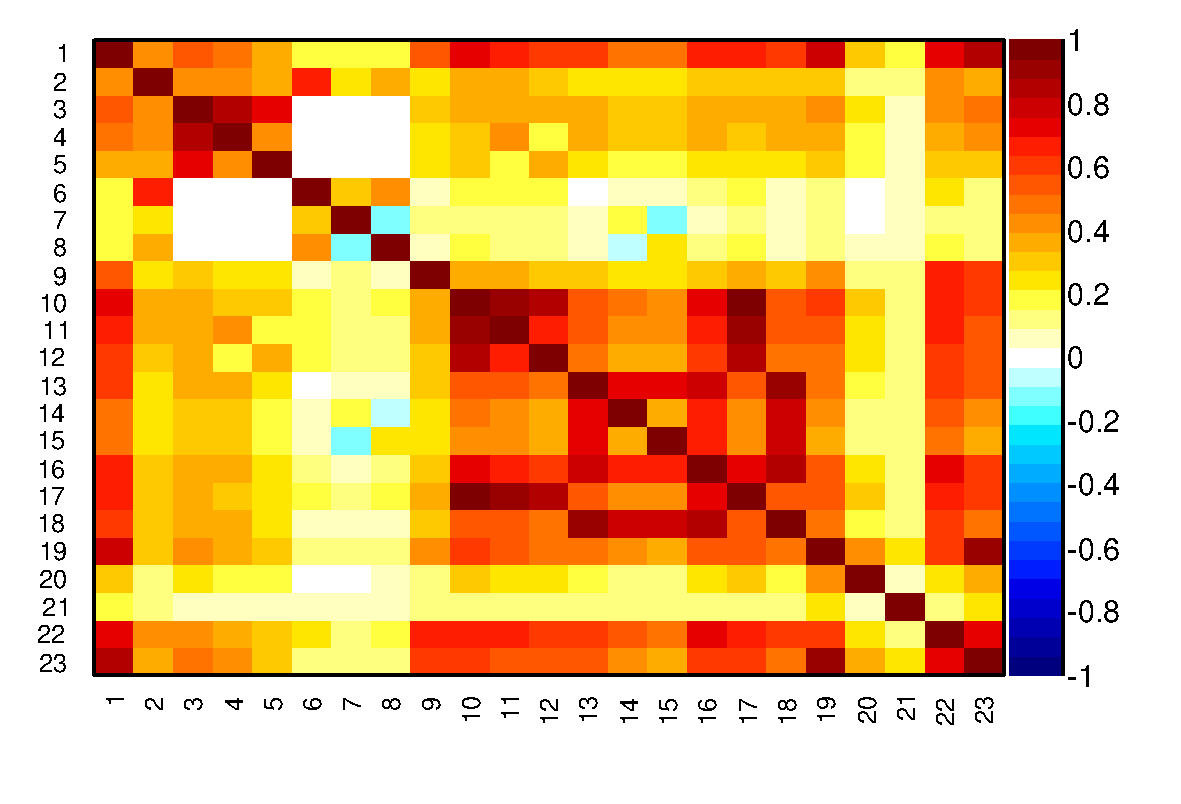
\includegraphics[width=0.8\textwidth]{RKst/figs/Training/muons/correlation.pdf}
%\caption{Graphical representation of correlation matrix between truth and neural network inputs.
%Column/row number 1 is correlation to the truth (whether candidate is signal or background). All
%others give correlation between inputs with numbering scheme corresponding to the id column of
%Tab.~\ref{tab:RKst_nnInputs}. Correlation is calculated using all events without distinguishing signal and
%background.}
%\label{fig:Rkst_nnCorrelation}
%\end{figure}
%

Figure~\ref{fig:RKst_nnDist} shows neural network output distributions for signal and background.
On this plot the distributions from the test samples are also overlaid in order to check for overtraining. 
The distributions follow the same shape but with different fluctuations indicating no
significant overtraining. In general it can be concluded that the neural network is able to separate signal
from background and that the training converged properly.

If too much information is given to the classifier, this can become able to 
calculate the invariant mass of the candidates from its input variables. This could generate fake peaks and it is therefore
important to check for correlations between the 4-body invariant mass and the neural-network output. Figure~\ref{fig:RKst_NNprofiles} 
shows the average neural-network output as a function of the 4-body mass for sideband data and simulated signal candidates.
The distributions are flat showing that no significant correlation is present.


\subsection{Optimisation}
\label{sec:optimisation}

\begin{figure}[t!]
\centering
\includegraphics[width=0.49\textwidth]{RKst/figs/Optimisation/optimizeCut_MM-q2central/fitB_MM_0.pdf}
\includegraphics[width=0.49\textwidth]{RKst/figs/Optimisation/optimizeCut_EE-q2central/fitB_EE_0.pdf}
\caption{Fit to the data sidebands performed to estimate the amount of residual background in the
signal mass window for (left) muons and (right) electrons. The region corresponding to the dashed line is excluded from the fit.}
\label{fig:sideband_fit}
\end{figure}

In order to optimise the requirements on the \mbcm and the neural network output the expected
signal significance, $N_{\mathrm{S}}/\sqrt{N_{\mathrm{S}}+N_{\mathrm{B}}}$, is maximised,
where $N_\mathrm{S}$ ($N_\mathrm{B}$) is the number of rare signal (background) candidates.
When the BCM requirement is applied, the optimisation is performed in a three-dimensional space
($t_{\rm MVA}$, $a_{\rm BCM}$, $b_{\rm BCM}$), where $t_{\rm MVA}$ is the neural-network output threshold below which
a candidate is considered background, and $a_{\rm BCM}$ and $b_{\rm BCM}$ are the parameters of the BCM
cut described in Sec.~\ref{sec:HOP}. Otherwise, only the MVA cut is optimised 
(this is the case for all muons samples and the high-\qsq electron sample).

%The number of signal events accepted for a given neural-network output cut is determined with a data-driven method
%with exploits the resonant channel. First, as an arbitrary number of events can be simulated, this has to be rescaled
%to the expected yield. This is done by fitting \decay{\Bz}{\Kstarz(\jpsi\to\ll)} candidates after pre-selection,
%including all requirements except MVA. The resonant yield is then scaled down by the expected ratio between
%the rare and the resonant channels. The number of background events is instead derived by fitting the combinatorial
%background in the sideband with an exponential function and extrapolating the fit function below the signal peak.

\begin{figure}[h!]
\centering
\includegraphics[width=0.49\textwidth]{RKst/figs/Training/EE_wNB_vs_MPV_bkg.pdf}
\includegraphics[width=0.49\textwidth]{RKst/figs/Training/MM_wNB_vs_MPV_bkg.pdf}
\includegraphics[width=0.49\textwidth]{RKst/figs/Training/EE_wNB_vs_MPV_sgn.pdf}
\includegraphics[width=0.49\textwidth]{RKst/figs/Training/MM_wNB_vs_MPV_sgn.pdf}
\caption{Average value of neural network output as a function of 4-body invariant mass for data
sideband (top) and simulated signal (bottom) candidates for the electron (left) and muon (right) trainings.}
\label{fig:RKst_NNprofiles}
\end{figure}
%
%
\begin{figure}[h!]
\centering
\includegraphics[width=0.49\textwidth]{RKst/figs/Optimisation/optimizeCut_EE-q2central/EE_Optimize_t_MVA.pdf}
\includegraphics[width=0.49\textwidth]{RKst/figs/Optimisation/optimizeCut_MM-q2central/MM_Optimize_t_MVA.pdf}
\includegraphics[width=0.49\textwidth]{RKst/figs/Optimisation/optimizeCut_EE-q2central/EE_ROC_t_MVA.pdf}
\includegraphics[width=0.49\textwidth]{RKst/figs/Optimisation/optimizeCut_MM-q2central/MM_ROC_t_MVA.pdf}
\caption{(top) Dependence of figure-of-merit on the requirement on neural network output.
(bottom) Signal efficiency versus background rejection.
Plots correspond to the electron (left) and muons (right) samples.}
\label{fig:RKst_FOM}
\end{figure}

The number of signal candidates accepted by a given requirement is determined using a data-driven method.
Firstly, \mbox{\BdToKstJPsll} candidates selected with all the requirements except for the MVA, and BCM cuts 
are fitted to determine the total yield. 
% (see Fig.~\ref{fig:RKst_sW_mass}).
This number is then scaled by the ratio between the signal and \mbox{\BdToKstJPsll} branching fractions and
the efficiency ratio: 
%as a function of the cut
%
$$N_{\mathrm{S}} = N_{\jpsi(\ell\ell)} \cdot
\frac{\BR(\mathrm{S})}{\BR(\BdToKstJPsll)} \cdot
\frac{\varepsilon_{\mathrm{S}}}{\varepsilon_{\jpsi(\ell\ell)}} \, .$$

The number of background candidates is also derived from data by fitting the background in the lower and upper 
mass sidebands with an exponential function, and extrapolating the residual yield in the signal region (Fig.~\ref{fig:sideband_fit}).
Because the background shape changes as a function of the requirement that is being optimised, the sidebands are refitted for each considered cut value.
%
%$$N_{\mathrm{B}} \propto N_{\mKpill < 5000 \,||\, \mKpill > 5500} \, .$$

The cut optimisation is performed in a signal mass window of $\pm100~\mevcc$ around the nominal \Bz mass for muons, and between 5000 and 5400~\mevcc~ for electrons.
The average result of the $k$ optimisations is taken as the nominal requirement.
%
%
%
The variation of the signal and background efficiency, signal purity and figure-of-merit as a function of the neural-network output
requirement for the central-\qsq is shown in Fig.~\ref{fig:RKst_FOM}
together with curves of the background rejection as a function of the signal efficiency.
%
%Using the described MVA cuts the signal efficiency is $\sim 95\%$ for the muon channels
%and $\sim 93\%$ for the electron channels (for more details see Sec.~\ref{sec:RKst_efficiency}),
%while the background rejections is $\sim 97\%$ on both samples.
%
After the full selection about $\sim 3\%$ of events still contain multiple candidates
which are removed at random to retain only a single candidate per event.

\clearpage

\subsection{Selection summary}

Table~\ref{tab:sel_summary} summarises the requirements applied for each sample 
on top of the pre-selection requirements described in Sec.~\ref{sec:RKst_trigstripping}.

\begin{table}[ht!]
\begin{center}
\caption{Summary of the selection requirements. The last column
indicates to  which \qsq intervals the requirement is applied.}
\label{tab:sel_summary}
\begin{footnotesize}
\renewcommand\arraystretch{1.4}
\begin{tabular}{c|c|c|c}
\multicolumn{2}{c|}{\textbf{Type}} & \textbf{Requirement} & {\boldmath\qsq} \\
\hline
\multirow{2}{*}{Quality} & \multirow{2}{*}{All tracks}
	& $\chisqndf < 3$ & all \\
	&& {\verb GhostProb } $< 0.4$ & all \\
\hline
ID & \Kstarz & $|m(\kaon\pi) - m_{\Kstarz}^{PDG}| < 100\mevcc$ & all \\
\hline
 \multirow{4}{*}{PID}
	& $K$	& $\texttt{ProbNNk} \cdot (1 - \texttt{ProbNNp}) > 0.05$ & all \\
	& $\pi$	& $\texttt{ProbNNpi} \cdot (1 - \texttt{ProbNNk}) \cdot (1 - \texttt{ProbNNp}) > 0.1$ & all \\
	& $\mu$	& $min(\texttt{ProbNNmu}) > 0.2$ & all $\mu\mu$ \\
	& $e$	& $min(\texttt{ProbNNe}) > 0.2$ & all $ee$ \\
	\hline
	\multirow{19}{*}{BKG}
	& Swap & $|m((\decay{h}{\mu})\mu) - m_{\jpsi, (\psitwos)}^{PDG}| > 60\mevcc$ & all \\
	& \BuToKll & $max(m(K\ell\ell),m((\decay{\pi}{\kaon})\ell\ell)) < 5.1\gevcc$ & all \\
	& \BsToPhill & $m(K(\decay{\pi}{K})) > 1040~\mevcc$ & all \\
	& \decay{\Bd}{\Dm\ep\nu} & $|\cos\theta_\ell\,| < 0.8$ & except high- \\
%	& \BdToKstGee & $\sigma_{Z}(\epem) < 30~\rm{mm}$ & only low- \\
	& \BdToKstG & $\sigma_{z}(\ee) < 30~\rm{mm}$ & except $\gamma(ee)$ \\
\cline{2-4}
	& \multirow{10}{*}{Comb}	& $\texttt{NNout} > 0.68$ & $\mu\mu$ low- \\
	&					& $\texttt{NNout} > 0.64$ & $ee$ low- \\
	& 					& $\texttt{NNout} > 0.85$ & $\mu\mu$ central- \\
	&					& $\texttt{NNout} > 0.97$ & $ee$ central- \\
	& 					& $\texttt{NNout} > 0.40$ & $\mu\mu$ high- \\
	&					& $\texttt{NNout} > 0.93$ & $ee$ high- \\
\cline{3-4}
	& 					& $\texttt{NNout} > 0.06$ & $\jpsi(\mu\mu)$ \\
	&					& $\texttt{NNout} > 0.20$ & $\jpsi(ee)$\\
\cline{3-4}
	&					& $\texttt{NNout} > 0.16$ & $\gamma(ee)$ \\
%	&					& $\texttt{NNout} > 0.36$ & \JPsee \mKpiee \\
	&					& $\texttt{NNout} > 0.68$ & $\psitwos(ee)$ \\
\cline{2-4}
	& Part-reco					& $m(K\pi\ell\ell)_\jpsi	> 5150$~\mevcc		& $\jpsi(ee)$	\\
\cline{2-4}
	& \multirow{3}{*}{Comb, part-reco}	& $\mbcm > 4680 + 31 \cdot \log(\chisq_{\rm FD})$ & $ee$ low- \\
	&							& $\mbcm > 4437 + 64 \cdot \log(\chisq_{\rm FD})$ & $ee$ central- \\
\cline{3-4}	
	&							& $\mbcm > 3380 + 140 \cdot \log(\chisq_{\rm FD})$ & $\gamma(ee)$ \\
%	&							& $\mbcm > 2714 + 164 \cdot \log(\chisq_{\rm FD})$ & $\jpsi(ee)$ \\	
\end{tabular}
\end{footnotesize}
\end{center}
\end{table}



\section{Peaking backgrounds}
\label{sec:physbg}
 In addition to combinatorial background formed from the random
 combination of particles, backgrounds due to specific decays are
 studied using fully reconstructed samples of simulated \bquark hadron
 decays in which the final state includes two muons.  For the
 \decay{\Lb}{\jpsi\Lz} channel, the only significant contribution is
 from \decay{\Bz}{\jpsi\KS} decays, with \decay{\KS}{\pip\pim} where
 one of the pions is misidentified as a proton.  This decay contains a
 long-lived \KS meson and therefore has the same topology as the
 \decay{\Lb}{\jpsi\Lz} mode. This contribution leads to a broad shape
 that peaks below the \Lb mass region, which is taken into account in
 the mass fit.

 For the \decay{\Lb}{\Lz\mumu} channel two sources of peaking
 background are identified. The first of these is
 \decay{\Lb}{\jpsi\Lz} decays in which an energetic photon is radiated
 from either of the muons; this constitutes a background in the \qsq
 region just below the square of the \jpsi mass and in a mass region
 significantly below the \Lb mass.  These events do not contribute
 significantly in the \qsq intervals chosen for the analysis.  The
 second source of background is due to \decay{\Bz}{\KS\mumu} decays,
 where \decay{\KS}{\pip\pim} and one of the pions is misidentified as
 a proton.  This contribution is estimated by scaling the number of
 \decay{\Bz}{\jpsi\KS} events found in the \decay{\Lb}{\jpsi\Lz} fit
 by the ratio of the world average branching fractions for the decay
 processes \decay{\Bz}{\KS\mumu} and \decay{\Bz}{\jpsi(\to\mumu)\KS}
 \cite{Agashe:2014kda}.  Integrated over \qsq this is estimated to
 yield fewer than ten events, which is small relative to the expected
 total background level.

\section{Yields}

\subsection{Fit procedure}
 The yields of signal and background events in the data are
 determined in the mass range 5.35--6.00\gevcc using unbinned
 extended maximum likelihood fits for the \decay{\Lb}{\Lz\mumu} and
 the \decay{\Lb}{\jpsi\Lz} modes.  The likelihood function has the form
\begin{equation}
\mathcal{L}=e^{-(N_\mathrm{S}+N_\mathrm{C}+N_{\mathrm{P}})} \times \prod_{i=1}^{N}[
  N_\mathrm{S}P_{\mathrm{S}}(m_i)+N_\mathrm{C}P_\mathrm{C}(m_i)+N_{\mathrm{P}}P_{\mathrm{P}}(m_i)]
 \;,
\label{eq:uml}
\end{equation}
 \noindent where $N_\mathrm{S}$, $N_\mathrm{C}$ and $N_\mathrm{P}$ are
 the number of
 signal, combinatorial and peaking background events, respectively, 
 $P_j(m_i)$ are the corresponding probability density functions
 (PDFs) and $m_i$  is the mass of the \Lb candidate. 
 The signal yield itself is parametrised in the fit using the
 relative branching fraction of the signal and normalisation modes,
%
\begin{equation}
N_\mathrm{S}(\Lz\mumu)_{k}  = \left[ \frac{\mathrm{d}\mathcal{B}(\Lz\mumu)/\mathrm{d}\qsq}{\mathcal{B}(\jpsi\Lz)} \right]  \cdot
N_\mathrm{S}(\jpsi\Lz)_{k} \cdot \varepsilon^{\mathrm{rel}}_{k} \cdot \frac {\Delta\qsq} { \mathcal{B}(\jpsi\to\mumu) },
\label{eq:ield_from_BR}
\end{equation}
\noindent
where $k$ is the candidate category (long or downstream), $\Delta\qsq$
is the width of the \qsq interval considered and
$\varepsilon_k^{\mathrm{rel}}$ is the relative efficiency, fixed to
the values obtained as described in Sec.~\ref{sec:efficiency}. Fitting
the ratio of the branching fractions of signal and normalisation modes
simultaneously in both candidate categories makes better statistical
use of the data.

 The signal shape, in both \decay{\Lb}{\Lz\mumu} and
 \decay{\Lb}{\jpsi\Lz} modes, is described by the sum of two Crystal
 Ball functions~\cite{Skwarnicki:1986xj} that share common means and
 tail parameters but have independent widths.  The combinatorial
 background is parametrised by an exponential function, independently
 in each \qsq interval. The background due to \decay{\Bz}{\jpsi\KS}
 decays is modelled by the sum of two Crystal Ball functions with
 opposite tails. All shape parameters are independent
 for the downstream and long sample.

 For the \decay{\Lb}{\jpsi\Lz} mode, the widths and common mean in the
 signal parametrisation are free parameters. The parameters describing
 the shape of the peaking background are fixed to those derived from
 simulated \decay{\Bz}{\jpsi\KS} decays, with only the normalisation
 allowed to vary to accomodate differences between data and simulation.

 For the \decay{\Lb}{\Lz\mumu} decay, the signal shape parameters are
 fixed according to the result of the fit to \decay{\Lb}{\jpsi\Lz}
 data and the widths are rescaled to allow for possible differences
 in resolution as a function of \qsq. The scaling factor is determined
 comparing \decay{\Lb}{\jpsi\Lz} and \decay{\Lb}{\Lz\mumu} simulated events.
 %The ratio between the widths of the two Crystal Ball functions 
 %summed to obtain the signal PDF is constrained to
 %that obtained from the normalisation mode, with a common scale
 %factor, determined from a fit to simulated \decay{\Lb}{\Lz\mumu}
 %events, allowing for possible differences in resolution as a function
 %of \qsq.  
 The \decay{\Bz}{\KS\mumu} background component is also
 modelled using the sum of two Crystal Ball functions with opposite
 tails where both the yield and all shape parameters are constrained
 to those obtained from simulated events.
 
\subsection{Fit results}
 The invariant mass distribution of the \decay{\Lb}{\jpsi\Lz}
 candidates selected with the high-\qsq requirements is shown in
 Fig.~\ref{fig:totalFit}, combining both long and downstream
 candidates.  The normalisation channel candidates are divided into
 four sub-samples: downstream and long events are fitted separately
 and each sample is selected with both the low-\qsq and high-\qsq
 requirements to normalise the corresponding \qsq regions in signal.
 The number of \decay{\Lb}{\jpsi\Lz} decays found in each case
 is given in Table~\ref{tab:jpsi_yield}.
%
\begin{table}[tbp]
\centering
\caption{Number of \decay{\Lb}{\jpsi\Lz} decays in the long and
  downstream categories found using the selection for low- and
  high-\qsq regions. Uncertainties shown are statistical only.}
\begin{tabular}{lcc}
Selection & $N_{\rm S}$ (long) & $N_{\rm S}$ (downstream)\\ \hline
high-\qsq	& $4313 \pm 70$	 	&  $11\,497 \pm 123$ \\
low-\qsq	& $3363 \pm 59$ 	&  $\phantom{0}\,7225 \pm 89\phantom{0}$  \\
 \hline
\end{tabular}
\label{tab:jpsi_yield}
\end{table}
%
\begin{figure}[tpbh!]
%%\centering \includegraphics[width=0.8\textwidth]{images_and_tables/BR/fit_Jpsi_All_log.pdf}
\centering \includegraphics[width=0.8\textwidth]{figure1.pdf}
\caption{\small Invariant mass distribution of the \decay{\Lb}{\jpsi\Lz}
  candidates selected with the neural network requirement used for the high-\qsq region.
  The (black) points show data, combining downstream
  and long candidates, and the solid (blue) line represents the
  overall fit function.  The dotted (red) line represents the combinatorial
  and the dash-dotted (brown) line the peaking background from
  \decay{\Bz}{\jpsi\KS} decays.}
\label{fig:totalFit}
\end{figure}

  The fraction of peaking background events is larger in the
  downstream sample amounting to 28\,\% of the \decay{\Lb}{\jpsi\Lz} yield in the
  full fitted mass range, while in the sample of long candidates it
  constitutes about 4\,\%.

  The invariant mass distributions for the \decay{\Lb}{\Lz\mumu}
  process, integrated over $15.0<\qsq<20.0$\gevgevcccc and in eight
  separate \qsq intervals, are shown in Figs.~\ref{fig:totalFitRare}
  and \ref{fig:differentialFit}.  The yields found in each \qsq
  interval are given in Table~\ref{tab:rareYields} together with their
  significances.  The statistical significance of the observed signal
  yields is evaluated as $\sqrt{2\Delta\ln{\mathcal{L}}}$, where
  $\Delta\ln{\mathcal{L}}$ is the change in the logarithm of the
  likelihood function when the signal component is excluded from the
  fit, relative to the nominal fit in which it is present.

\begin{figure}[tbph!]
%%\centering \includegraphics[width=0.8\textwidth]{images_and_tables/BR/fit_All_highQ2.pdf}
\centering \includegraphics[width=0.8\textwidth]{figure2.pdf}
\caption{\small Invariant mass distribution of the
  \decay{\Lb}{\Lz\mumu} candidates, integrated over the region  $15.0 < \qsq < 20.0$ \gevgevcccc 
  together with the fit function described in the text.  The points show data,
  the solid (blue) line is the overall fit function and the dotted
  (red) line represents the combinatorial background.
  The background component from \decay{\Bz}{\KS\mumu} decays, (brown)
  dashed line, is barely visibile due to the very low yield.}
\label{fig:totalFitRare}
\end{figure}
%
\begin{figure}[tbph]
%%\centering \includegraphics[width=0.64\textheight]{images_and_tables/BR/q2_fits_All_vertical.pdf}
\centering \includegraphics[width=0.64\textheight]{figure3.pdf}
\caption{\small Invariant mass distributions of \decay{\Lb}{\Lz\mumu}
candidates, in eight \qsq\ intervals, together with the
  fit function described in the text. The points show data, the
  solid (blue) line is the overall fit function and
  the dotted
  (red) line represents the combinatorial background component.}
\label{fig:differentialFit}
\end{figure}
%
\begin{table}[btph!]
\centering
\caption{\small Signal decay yields ($N_\mathrm{S}$) obtained from the
  mass fit to \decay{\Lb}{\Lz\mumu} candidates in each \qsq interval
  together with their statistical significances. 
  The yields are the sum of long and downstream categories with
  downstream decays comprising $\sim 80\,\%$ of the total yield.
  The $8-11$ and $12.5-15$ \gevgevcccc ~\qsq intervals are excluded
  from the study as they are dominated by decays via charmonium resonances.
  }
\label{tab:rareYields}
\begin{tabular}{ccc}
 $q^2$ interval [\gevgevcccc] & Total signal yield & Significance \\ \hline
0.1 -- 2.0    &  $16.0\pm5.3$            &  4.4 \\
2.0 -- 4.0    &  $\phantom{0}4.8\pm4.7$  &  1.2 \\
4.0 -- 6.0    &  $\phantom{0}0.9\pm2.3$  &  0.5 \\
6.0 -- 8.0    &  $11.4\pm5.3$            &  2.7 \\
11.0 -- 12.5  &  $\phantom{.0}60\pm12\phantom{.}$           &  6.5 \\
15.0 -- 16.0  &  $57\pm9$                &  8.7 \\
16.0 -- 18.0  &  $118\pm13$              &  13  \\
18.0 -- 20.0  &  $\phantom{.}100\pm11\phantom{.}$   &  14  \\
\hline
1.1 -- 6.0    &  $\phantom{0}9.4\pm6.3$  &  1.7 \\
15.0 -- 20.0  &  $276\pm20$              &  21  \\
\end{tabular}  
\end{table}

%\clearpage


 \section{Relative efficiency}
\label{sec:efficiency}

 The measurement of the differential branching fraction of
 \decay{\Lb}{\Lz\mumu} relative to \decay{\Lb}{\jpsi\Lz} benefits from
 the cancellation of several potential sources of systematic
 uncertainty in the ratio of efficiencies, $\varepsilon^{\rm
   rel}=\etot(\decay{\Lb}{\Lz\mumu})/\etot(\decay{\Lb}{\jpsi\Lz})$.
 Due to the long lifetime of \Lz baryons, most of the candidates are
 reconstructed in the downstream category, with an overall efficiency
 of 0.20\,\%, while the typical efficiency is 0.05\,\% for long
 candidates.

 The efficiency of the PID is obtained from a data-driven
 method~\cite{LHCb-DP-2012-003} and found to be 98\,\% while all other
 efficiencies are evaluated using simulated data.  The models used for
 the simulation are summarised in Sec.~\ref{sec:Detector}.  The
 trigger efficiency is calculated using simulated data and increases
 from approximately 56\,\% to 86\,\% between the lowest and highest
 \qsq regions. An independent cross-check of the trigger efficiency is
 performed using a data-driven method.  This exploits the possibility
 of categorising a candidate \decay{\Lb}{\Lz\mumu} or
 \decay{\Lb}{\jpsi\Lz} decay in two ways depending on which tracks are
 directly responsible for its selection by the trigger: {``trigger on
   signal''} candidates, where the tracks responsible for the
 {hardware and software} trigger decisions are associated with the
 signal; and {``trigger independent of signal''} candidates, with a
 \Lb baryon reconstructed in either of these channels but where the
 trigger decision does not depend on any of their decay products.  As
 these two categories of event are not mutually exclusive, their
 overlap may be used to estimate the efficiency of the trigger
 selection using data.  Using \decay{\Lb}{\jpsi\Lz} candidates and
 calculating the ratio of yields that are classified as both trigger
 on signal and independent of signal, relative to those that are
 classified as trigger independent of signal, an efficiency of
 $(70\pm5)$\,\% is obtained, which is consistent with that of
 $(73.33\pm0.02)$\,\% computed from simulation.

 The relative efficiency for the ratio of branching fractions in each
 \qsq interval, calculated from the absolute efficiencies described
 above, is shown in Fig.~\ref{fig:relativeTotalEfficiency}.
 The increase in efficiency as a function of increasing \qsq is
 dominated by two effects. Firstly, at low \qsq the muons have lower
 momenta and therefore have a lower probability of satisfying the
 trigger requirements.  Secondly, at low \qsq the \Lz baryon has a
 larger fraction of the \Lb momentum and is more likely to decay
 outside of the acceptance of the detector. 
 Separate selections are used for the low- and high-\qsq regions and,
 as can be seen in Fig.~\ref{fig:relativeTotalEfficiency}, the tighter
 neural network requirement used in the low-\qsq region has
 a stronger effect on downstream candidates.
 
 The uncertainties combine both
 statistical and systematic contributions (with the latter dominating)
 and include a small correlated uncertainty due to the use of a single
 simulated sample of \decay{\Lb}{\jpsi\Lz} decays as the normalisation channel
 for all \qsq\ intervals.  Systematic uncertainties associated with the
 efficiency calculation are described in detail in Sec.~\ref{sec:systemtics}.

\begin{figure}[tbp]
%\centering \includegraphics[width=0.8\textwidth]{images_and_tables/BR/Efficiency.pdf}
\centering \includegraphics[width=0.8\textwidth]{figure4.pdf}
\caption{\small
Total relative efficiency,
$\varepsilon_{\mathrm{rel}}$, between \decay{\Lb}{\Lz\mumu} and
\decay{\Lb}{\jpsi\Lz} decays.
The uncertainties are the combination of
both statistical and systematic components, and are dominated by the
latter.}
\label{fig:relativeTotalEfficiency}
\end{figure}

\section{Systematic uncertainties on the branching fraction}
\label{sec:systemtics}
\subsection{Yields}
\label{sec:systematics_yields}
 Three sources of systematic uncertainty on the measured yields are
 considered for both the \decay{\Lb}{\jpsi\Lz} and the
 \decay{\Lb}{\Lz\mumu} decay modes: the shape of the signal PDF, the
 shape of the background PDF and the choice of the fixed parameters
 used in the fits to data.

 For both decays, the default signal PDF is replaced by the sum of two
 Gaussian functions. All parameters of the Gaussian functions are
 allowed to vary to take into account the effect of fixing
 parameters. The shape of the background function is changed by
 permitting the \KS\mumu peaking background yield, which is fixed to
 the value obtained from simulation the nominal fit, to vary.  For the
 resonant channel, the \jpsi\KS peaking background shape is changed by
 fixing the global shift to zero.  Finally, simulated experiments are
 performed using the default model, separately for each \qsq interval,
 generating the same number of events as observed in data.  Each
 distribution is fitted with the default model and the modified
 PDFs. The average deviation over the ensemble of simulated
 experiments is assigned as the systematic uncertainty.  The relative
 change in signal yield due to the choice of signal PDF varies between
 0.6\,\% and 4.6\,\% depending on \qsq, while the change due to the
 choice of background PDF is in the range between 1.1\,\% and
 2.5\,\%. The \qsq intervals that are most affected are those in which
 a smaller number of candidates is observed and therefore there are
 fewer constraints to restrict potentially different PDFs.  The
 systematic uncertainties on the yield in each \qsq interval are
 summarised in Table~\ref{tab:brsys}, where the total is the sum in
 quadrature of the individual components.

\subsection{Relative efficiencies}
 \label{sec:systematics_eff}
 The dominant systematic effect is that related to the current
 knowledge of the angular structure and the \qsq dependence of the
 decay channels.  The uncertainty due to the finite size of simulated
 samples is comparable to that from other sources. The total
 systematic uncertainties on the efficiencies, calculated as the sums
 in quadrature of the individual components described below,
 are summarised in Table~\ref{tab:brsys}.


\subsubsection{Decay structure and production polarisation}
 The main factors that affect the detection efficiencies are the
 angular structure of the decays and the production polarisation
 ($P_b$). Although these arise from different parts of the process,
 the efficiencies are linked and are therefore treated together.

 For the \decay{\Lb}{\Lz\mumu} decay, the impact of the limited
 knowledge of the production polarisation, $P_b$, is estimated by
 comparing the default efficiency, obtained in the unpolarised
 scenario, with those in which the polarisation is varied within its
 measured uncertainties, using the most recent LHCb measurement, $P_b
 = 0.06 \pm 0.09$\cite{LHCb-PAPER-2012-057}.  The larger of these
 differences is assigned as the systematic uncertainty from this
 source. This yields a $\sim 0.5\,\%$ uncertainty on the efficiency of
 downstream candidates and $\sim 1.2\,\%$ for long candidates.  No
 significant \qsq dependence is found.

 To assess the systematic uncertainty due to the limited knowledge of
 the decay structure, the efficiency corresponding to the default
 model \cite{Gutsche:2013pp,Aliev:2005np,Buras:1994dj} is compared to
 that of a model containing an alternative set of form factors based
 on a lattice QCD calculation \cite{Detmold:2012vy}. The larger of the
 full difference or the statistical precision is assigned as the
 systematic uncertainty.
 
 For the \decay{\Lb}{\jpsi\Lz} mode, the default angular distribution
 is based on that observed in Ref.  \cite{LHCb-PAPER-2012-057}. The
 angular distribution is determined by the production polarisation and
 four complex decay amplitudes. The central values from
 Ref.~\cite{LHCb-PAPER-2012-057} are used for the nominal result. To
 assess the sensitivity of the \decay{\Lb}{\jpsi\Lz} mode to the
 choice of decay model, the production polarisation and decay
 amplitudes are varied within their uncertainties, taking into account
 correlations.

 To assess the potential impact that physics beyond the SM might have
 on the detection efficiency, the $C_7$ and $C_9$ Wilson coefficients
 are modified by adding a non-SM contribution ($C_i \rightarrow C_i +
 C_i^{'}$). The $C_i^{'}$ added are inspired to maintain compatibility
 with the recent LHCb result for the $P'_5$ observable
 \cite{Descotes-Genon:2013wba} and indicate a change at the level of
 $\sim 7$\,\% in the 0.1--2.0 \qsq interval, and 2--3\,\% in other
 regions.  No systematic is assigned as a result of this study.

 \subsubsection{Reconstruction efficiency for the \Lz baryon}
 The \Lz baryon is reconstructed from either long or downstream
 tracks, and their relative proportions differ in data and simulation.
 This proportion does not depend significantly on \qsq and therefore
 possible effects cancel in the ratio with the normalisation channel.
 Furthermore, since the analysis is performed separately for long and
 downstream candidates, it is not necessary to assign a systematic
 uncertainty to account for a potential effect due to the different
 fractions of candidates of the two categories observed in data and
 simulation.  To allow for residual differences between data and
 simulation that do not cancel completely in the ratio between signal
 and normalisation modes, systematic uncertainties of 0.8\,\% and
 1.2\,\% are estimated for the low-\qsq and high-\qsq regions,
 respectively, using the same data-driven method as in
 Ref.~\cite{LHCb-PAPER-2014-006}.


 \subsubsection{Production kinematics and lifetime of the \Lb baryon}
  In \decay{\Lb}{\jpsi\Lz} decays a small difference is observed
  between data and simulation in the momentum and transverse momentum
  distributions of the \Lb baryon produced. Simulated data are
  reweighted to reproduce these distributions in data and the relative
  efficiencies are compared to those obtained using events that are
  not reweighted.  This effect is less than 0.1\,\%, which is
  negligible with respect to other sources.

  Finally, the \Lb baryon lifetime used throughout corresponds to the
  most recent \lhcb measurement, $1.479\pm0.019$\ps
  \cite{LHCb-PAPER-2014-003}.  The associated systematic uncertainty
  is estimated by varying the lifetime value by one standard deviation
  and negligible differences are found.


 \begin{table}[tbp]
 \centering
 \caption{Systematic uncertainties as a function of \qsq, assigned for
   yields and efficiencies. Values reported are the sums in quadrature
   of all contributions evaluated within each category. }
 \label{tab:brsys}
 \renewcommand{\arraystretch}{1.3}
 \begin{tabular}{ccc}
  %%Nigel Watson 20150212 $q^2$ interval [\gevgevcccc] & \multicolumn{2}{c}{\text{ } Syst. on
  %%Nigel Watson 20150212    eff. [\%] \text{ }} & Syst. on yields [\%] \\ \hline
 $q^2$ interval [\gevgevcccc]  & Syst.\ on yields [\%] & Syst.\ on
  eff. [\%] \\ \hline

0.1 -- 2.0  	 	& 3.4  &	 $_{-3.6}^{+2.2}$ 	  \\
2.0 -- 4.0  	 	& 3.8  &	 $_{-4.1}^{+2.2}$ 	  \\
4.0 -- 6.0  	 	& 6.6  &	 $_{-14.3}^{+17.2}$   \\
6.0 -- 8.0  	 	& 2.0  &	 $_{-3.1}^{+2.1}$ 	  \\
11.0 -- 12.5  	 	& 3.2  &	 $_{-5.2}^{+3.7}$ 	  \\
15.0 -- 16.0  	 	& 2.8  &	 $_{-2.8}^{+3.1}$ 	  \\
16.0 -- 18.0  	 	& 1.4  &	 $_{-4.1}^{+3.0}$ 	  \\
18.0 -- 20.0  	 	& 2.5  &	 $_{-2.3}^{+3.9}$ 	  \\
\hline
1.1 -- 6.0  	 	& 4.2  &	 $_{-4.6}^{+2.2}$ 	  \\
15.0 -- 20.0       	& 1.0  &    $_{-2.9}^{+2.0}$      \\

%%%%% Old table with no WC systematics
%0.1 -- 2.0       & 3.4 & $^{+6.4}_{-7.3}$\\
%2.0 -- 4.0       & 3.8 & $^{+4.9}_{-5.4}$\\
%4.0 -- 6.0       & 6.6 & $^{+1.9}_{-2.0}$\\
%6.0 -- 8.0       & 2.0 & $^{+3.8}_{-4.1}$\\
%11.0 -- 12.5     & 3.2 & $^{+3.2}_{-3.4}$\\
%15.0 -- 16.0     & 2.8 & $^{+3.5}_{-3.8}$\\
%16.0 -- 18.0     & 1.4 & $^{+3.1}_{-3.3}$\\
%18.0 -- 20.0     & 2.5 & $^{+3.1}_{-3.3}$\\
%\hline                                 
%1.1 --  6.0      & 4.2 & $^{+5.3}_{-6.0}$\\
%15.0 -- 20.0     & 1.0 & $^{+1.8}_{-1.9}$\\
\end{tabular}
\end{table}



\section{Differential branching fraction}
 The values for the absolute branching fraction of the
 \decay{\Lb}{\Lz\mumu} decay, obtained by multiplying the relative
 branching fraction by the absolute branching fraction of the
 normalisation channel,
 $\BF(\decay{\Lb}{\jpsi\Lz})=(6.3\pm1.3)\times10^{-4}$~\cite{Agashe:2014kda},
 are given in Fig.~\ref{fig:mass_fit_smallbins} and summarised in
 Table~\ref{tab:AbsBR}, where the SM predictions are obtained from
 Ref.~\cite{Detmold:2012vy}.  The relative branching fractions are
 given in the Appendix.

 Evidence for signal is found in the \qsq region between the
 charmonium resonances and in the interval $0.1 < \qsq < 2.0$
 \gevgevcccc, where an increased yield is expected due to the
 proximity of the photon pole.  The uncertainty on the branching
 fraction is dominated by the precision of the branching fraction for
 the normalisation channel, while the uncertainty on the relative
 branching fraction is dominated by the size of the data sample
 available.  The data are consistent with the theoretical predictions
 in the high-\qsq region but lie below the predictions in the low-\qsq
 region.

\begin{table}[tbph]
\centering
\renewcommand{\arraystretch}{1.2}
\caption{Measured differential branching fraction of
  \decay{\Lb}{\Lz\mumu}, where the uncertainties are statistical, systematic and
 due to the uncertainty on the normalisation mode, \decay{\Lb}{\jpsi\Lz}, respectively.}
\begin{tabular}{ccccccc}
  \qsq interval  [\gevgevcccc] & &\multicolumn{5}{c}{$\deriv \BF(\decay{\Lb}{\Lz\mumu})/\deriv\qsq \cdot 10^{-7} [(\gevgevcccc)^{-1}]$} \\
\hline
0.1 -- 2.0    &    &0.36  &  $^{+\,0.12}_{-\,0.11}$   & $^{+\,0.02}_{-\,0.02}$ & $\pm\,0.07$ \\
2.0 -- 4.0    &    &0.11  &  $^{+\,0.12}_{-\,0.09}$   & $^{+\,0.01}_{-\,0.01}$ & $\pm\,0.02$ \\
4.0 -- 6.0    &    &0.02  &  $^{+\,0.09}_{-\,0.00}$   & $^{+\,0.01}_{-\,0.01}$ & $\pm\,0.01$ \\
6.0 -- 8.0    &    &0.25  &  $^{+\,0.12}_{-\,0.11}$   & $^{+\,0.01}_{-\,0.01}$ & $\pm\,0.05$ \\

11.0 -- 12.5  &    &0.75  &  $^{+\,0.15}_{-\,0.14}$   & $^{+\,0.03}_{-\,0.05}$ & $\pm\,0.15$ \\
15.0 -- 16.0  &    &1.12  &  $^{+\,0.19}_{-\,0.18}$   & $^{+\,0.05}_{-\,0.05}$ & $\pm\,0.23$ \\
16.0 -- 18.0  &    &1.22  &  $^{+\,0.14}_{-\,0.14}$   & $^{+\,0.03}_{-\,0.06}$ & $\pm\,0.25$ \\
18.0 -- 20.0  &    &1.24  &  $^{+\,0.14}_{-\,0.14}$   & $^{+\,0.06}_{-\,0.05}$ & $\pm\,0.26$ \\

\hline
1.1 -- 6.0    &    &0.09  &  $^{+\,0.06}_{-\,0.05}$   & $^{+\,0.01}_{-\,0.01}$ & $\pm\,0.02$ \\
15.0 -- 20.0  &    &1.20  &  $^{+\,0.09}_{-\,0.09}$   & $^{+\,0.02}_{-\,0.04}$ & $\pm\,0.25$ \\
 \end{tabular}
\label{tab:AbsBR}
\end{table}

 \begin{figure}[tbph]
 \centering
%% \includegraphics[width=0.8\textwidth]{images_and_tables/BR/combined_result_absolute_2err_rareErrIn.pdf}
 \includegraphics[width=0.8\textwidth]{figure5.pdf}
 \protect\caption{ Measured \protect\decay{\Lb}{\Lz\mumu} branching
   fraction as a function of \qsq with the predictions of the SM
   \cite{Detmold:2012vy} superimposed.  The inner error bars on data
   points represent the total uncertainty on the relative branching
   fraction (statistical and systematic); the outer error bar also
   includes the uncertainties from the branching fraction of the
   normalisation mode.}  \protect\label{fig:mass_fit_smallbins}
 \end{figure}


\section{Angular analysis}
The forward-backward asymmetries of both the dimuon system, $A_{\rm
  FB}^\ell$, and of the $p\pi$ system, $A_{\rm FB}^h$, are defined as
\begin{align}
A_{\rm FB}^i(\qsq)&=\frac{\int_0^1 \frac{\deriv^2\Gamma}{\deriv\qsq\,\deriv\!\cos\theta_i} \deriv\!\cos\theta_i-
               \int^0_{-1} \frac{\deriv^2\Gamma}{\deriv\qsq\,\deriv\!\cos\theta_i} \deriv\!\cos\theta_i}{\deriv\Gamma / \deriv \qsq},
\label{eq:afbTh}
\end{align}
\noindent
where $\deriv^2\Gamma/\deriv q^2\,\deriv\!\cos\theta_i$ is the
two-dimensional differential rate and $\deriv\Gamma/\deriv q^2$ is the
rate integrated over the corresponding angles.  The observables are
determined by a fit to one-dimensional angular distributions as a
function of $\cos \theta_\ell$, the angle between the positive
(negative) muon direction and the dimuon system direction in the
\Lb(\Lbbar) rest frame, and $\cos \theta_h$, which is defined as the
angle between the proton and the \Lz baryon directions, also in the
\Lb rest frame. The differential rate as a function of $\cos
\theta_\ell$ is described by the function
\begin{align}
\frac{\deriv^2\Gamma(\Lambda_{b}\to \Lambda \,\ell^{+}\ell^{-})}{\deriv\qsq\,\deriv\!\cos\theta_\ell}=
\frac{\deriv\Gamma}{\deriv\qsq}&\left[  \frac{3}{8}\left(1+\cos^2\theta_\ell\right)(1-f_{\rm L})+A_{\rm FB}^\ell\cos\theta_\ell +
   \frac{3}{4}f_{\rm L} \sin^2\theta_\ell \right], 
\label{eq:afbLTh}
\end{align}
where $f_{\rm L}$ is the fraction of longitudinally polarised dimuons.
 The rate as a function of $\cos \theta_h$ has the form
\begin{equation}
\frac{\deriv^2\Gamma(\Lambda_{b}\to \Lambda(\to p \pi^{-})\ell^{+}\ell^{-})}
     {\deriv\qsq\,\deriv\!\cos\theta_h} 
={\BF}(\Lambda \to p\pi^{-})
 \frac{\deriv\Gamma(\Lambda_b \to \Lambda\, \ell^{+}\ell^{-})}{\deriv \qsq}\frac{1}{2}
\Big(1+2A_{\rm FB}^h\cos\theta_h\Big) \,.
\label{eq:afbBTh}
\end{equation}
\noindent
These expressions assume that \Lb baryons are produced unpolarised,
which is in agreement with the measured production polarisation at
\lhcb~\cite{LHCb-PAPER-2012-057}.

The forward-backward asymmetries are measured in data using unbinned
maximum likelihood fits.  The signal PDF consists of a theoretical
shape, given by Eqs.~\ref{eq:afbLTh} and \ref{eq:afbBTh}, multiplied
by an acceptance function.  Selection requirements on the minimum
momentum of the muons may distort the $\cos \theta_\ell$ distribution
by removing candidates with extreme values of $\cos
\theta_\ell$. Similarly, the impact parameter requirements affect
$\cos \theta_h$ as very forward hadrons tend to have smaller impact
parameter values.  The angular efficiency is parametrised using a
second-order polynomial and determined separately for downstream and
long candidates by fitting simulated events, with an independent set
of parameters obtained for each \qsq interval. These parameters are
fixed in the fits to data.  The acceptances are shown in
Fig.~\ref{fig:AngEff} as a function of $\cos\theta_h$ and
$\cos\theta_\ell$ in the $15 < \qsq <20$ \gevgevcccc interval for each
candidate category.

The background shape is parametrised by the product of a linear
function and the signal efficiency, with the value of the slope
determined by fitting candidates in the upper mass sideband,
$m(\Lz\mumu) > 5700$ \mevcc.  To limit systematic effects due to
uncertainties in the background parametrisation, an invariant mass
range that is dominated by signal events is used: $5580 < m(\Lz\mumu)
< 5660 $ \mevcc.  The ratio of signal to background events in this
region is obtained by performing a fit to the invariant mass
distribution in a wider mass interval.
\begin{figure}[tbp]
\centering
%%\includegraphics[width=0.45\textwidth]{images_and_tables/Angular/LLeffFit_q2_1500_2000.pdf}
%%\includegraphics[width=0.45\textwidth]{images_and_tables/Angular/LLeffFitB_q2_1500_2000.pdf}
%%\includegraphics[width=0.45\textwidth]{images_and_tables/Angular/DDeffFit_q2_1500_2000.pdf}
%%\includegraphics[width=0.45\textwidth]{images_and_tables/Angular/DDeffFitB_q2_1500_2000.pdf}
\includegraphics[width=0.45\textwidth]{figure6a.pdf}
\includegraphics[width=0.45\textwidth]{figure6b.pdf}
\includegraphics[width=0.45\textwidth]{figure6c.pdf}
\includegraphics[width=0.45\textwidth]{figure6d.pdf}

\caption{Angular efficiencies as a function of (left)
  $\cos\theta_\ell$ and (right) $\cos\theta_h$ for (upper) long and
  (lower) downstream candidates, in the interval $15 < \qsq < 20$
  \gevgevcccc, obtained using simulated events.  The (blue) line shows
  the fit that is used to model the angular acceptance in the fit to
  data. }
\label{fig:AngEff}
\end{figure}


\begin{figure}[tbp]
\centering
%%ncludegraphics[width=0.49\textwidth]{images_and_tables/Angular/fit_q2_1500_2000_All_cosThetaL.pdf}
%%ncludegraphics[width=0.49\textwidth]{images_and_tables/Angular/fit_q2_1500_2000_All_cosThetaB.pdf}
\includegraphics[width=0.49\textwidth]{figure7a.pdf}
\includegraphics[width=0.49\textwidth]{figure7b.pdf}
\caption{Angular distributions as a function of (left) $\cos
  \theta_\ell$ and (right) $\cos \theta_h$, for candidates in the
  integrated $15 < \qsq <20$ \gevgevcccc interval with the overall fit
  function overlaid (solid blue). The (red) dotted line represents the
  combinatorial background.}
\label{fig:AngDistrib}
\end{figure}

The angular fit is performed simultaneously for the samples of downstream and
long candidates, 
using separate acceptance and background functions for the two
categories while keeping the angular observables as shared parameters.
Angular distributions are shown in Fig.~\ref{fig:AngDistrib} where the
two candidate categories are combined. 

\section{Systematic uncertainties on angular observables}
\subsection{Angular correlations}
 To derive Eqs.~\ref{eq:afbLTh} and \ref{eq:afbBTh}, a uniform
 efficiency is assumed. However, non-uniformity is observed,
 especially as a function of $\cos\theta_h$ (see
 Fig.~\ref{fig:AngEff}).  Therefore, while integrating over the full
 angular distribution, terms that would cancel with constant
 efficiency may remain and generate a bias in the measurement of these
 observables. To assess the impact of this potential bias, simulated
 experiments are generated in a two-dimensional ($\cos
 \theta_\ell$,$\cos \theta_h$) space according to the theoretical
 distribution multiplied by a two-dimensional efficiency histogram.
 Projections are then made and are fitted with the default
 one-dimensional efficiency functions. The average deviations from the
 generated parameters are assigned as systematic uncertainties. The
 magnitudes of these are found to be $-0.032$ for $A_{\rm FB}^\ell$,
 $0.013$ for $A_{\rm FB}^h$ and $0.028$ for $f_{\rm L}$, independently
 of \qsq.  In most \qsq intervals this is the dominant source of
 systematic uncertainty.


\subsection{Resolution}
 Resolution effects may induce an asymmetric migration of events
 between bins and therefore generate a bias in the measured value of
 the forward-backward asymmetries.  To study this systematic effect, a
 map of the angular resolution function is created using simulated
 events by comparing reconstructed quantities with those in the
 absence of resolution effects.  Simulated experiments are then
 generated according to the measured angular distributions and smeared
 using the angular resolution maps.  The simulated events, before and
 after smearing by the angular resolution function, are fitted with
 the default PDF.  The average deviations from the default values are
 assigned as systematic uncertainties.  These are larger for the
 $A_{\rm FB}^h$ observable because the resolution is poorer for
 $\cos\theta_h$ and the distribution is more asymmetric, yielding a
 net migration effect.  The uncertainties from this source are in the
 ranges $[0.011,0.016]$ for $A_{\rm FB}^\ell$, $[-0.001,-0.007]$ for
 $A_{\rm FB}^h$ and $[0.002,0.008]$ for $f_{\rm L}$, depending on
 \qsq.

\subsection{Angular acceptance}
 An imprecise determination of the efficiency due to data-simulation
 discrepancies could bias the $A_{\rm FB}$ measurement.  To estimate
 the potential impact arising from this source, the kinematic
 reweighting described in Sec.~\ref{sec:systematics_eff} is removed
 from the simulation.  Simulated samples are fitted using the same
 theoretical PDF multiplied by the efficiency function obtained with
 and without kinematical reweighting.  The average biases evaluated
 from simulated experiments are assigned as systematic uncertainties.
 These are larger for sparsely populated \qsq intervals and vary in
 the intervals $[0.009,0.016]$ for $A_{\rm FB}^\ell$, $[0.001,0.007]$
 for $A_{\rm FB}^h$ and $[0.002,0.044]$ for $f_{\rm L}$, depending on
 \qsq.

 The effect of the limited knowledge of the \Lb polarisation is
 investigated by varying the polarisation within its measured
 uncertainties, in the same way as for the branching fraction
 measurement. No significant effect is found and therefore no
 contribution is assigned.

\subsection{Background parametrisation}
\label{sec:bkgShapeSys}
As there is ambiguity in the choice of parametrisation for the
background model, in particular for regions with low statistical
significance in data, simulated experiments are generated from a PDF
corresponding to the best fit to data, for each \qsq interval. Each
simulated sample is fitted with two models: the nominal fit model,
consisting of the product of a linear function and the signal
efficiency, and an alternative model formed from a constant function
multiplied by the efficiency shape.  The average deviations are taken
as systematic uncertainties.  These are in the ranges $[0.003,0.045]$
for $A_{\rm FB}^\ell$, $[0.017,0.053]$ for $A_{\rm FB}^h$ and
$[0.014,0.049]$ for $f_{\rm L}$, depending on \qsq.


\section{Results of the angular analysis}
 The angular analysis is performed using the same \qsq intervals as
 those used in the branching fraction measurement.  Results are
 reported for each \qsq interval in which the statistical significance
 of the signal is at least three standard deviations. This includes
 all of the \qsq intervals above the \jpsi resonance and the lowest
 \qsq bin.

\begin{table}[tbp]
\centering
\caption{Measured values of leptonic and hadronic angular observables,
  where the first uncertainties are statistical and the second
  systematic.}
\label{tab:afbresults}
\renewcommand{\arraystretch}{1.2}
\begin{tabular}{c|ccc}
 \qsq interval  [\gevgevcccc]   &            $A_{\rm FB}^\ell$      &       $f_{\rm L}$ 						&  $A_{\rm FB}^h$                    \\ \hline

0.1 -- 2.0   & $\phantom{-\,}0.37 \; ^{+\;0.37}_{-\;0.48} \,\pm\, 0.03$  	&   $0.56 \; ^{+\;0.23}_{-\;0.56}\,\pm\, 0.08$ 		& $-\;0.12 \; ^{+\;0.31}_{-\;0.28}\,\pm\, 0.15$	\\
11.0 -- 12.5 & $\phantom{-\,}0.01 \; ^{+\;0.19}_{-\;0.18} \,\pm\, 0.06$  	&   $0.40 \; ^{+\;0.37}_{-\;0.36}\,\pm\, 0.06$		& $-\;0.50 \; ^{+\;0.10}_{-\;0.00}\,\pm\, 0.04$	 \\
15.0 -- 16.0 & $-\,0.10 \; ^{+\;0.18}_{-\;0.16} \,\pm\, 0.03$  			&   $0.49 \; ^{+\;0.30}_{-\;0.30} \,\pm\, 0.05$ 	& $-\;0.19 \; ^{+\;0.14}_{-\;0.16}\,\pm\, 0.03$	\\	
16.0 -- 18.0 & $-\,0.07 \; ^{+\;0.13}_{-\;0.12} \,\pm\, 0.04$  			&   $0.68 \; ^{+\;0.15}_{-\;0.21} \,\pm\, 0.05$ 	& $-\;0.44 \; ^{+\;0.10}_{-\;0.05}\,\pm\, 0.03$	\\
18.0 -- 20.0 & $\phantom{-\,}0.01 \; ^{+\;0.15}_{-\;0.14} \,\pm\; 0.04$  	&   $0.62 \; ^{+\;0.24}_{-\;0.27}\,\pm\, 0.04$ 		& $-\;0.13 \; ^{+\;0.09}_{-\;0.12}\,\pm\, 0.03$	\\ \hline
15.0 -- 20.0 & $-\,0.05 \; ^{+\;0.09}_{-\;0.09} \,\pm\, 0.03$  			&   $0.61 \; ^{+\;0.11}_{-\;0.14} \,\pm\, 0.03$ 	& $-\;0.29 \; ^{+\;0.07}_{-\;0.07}\,\pm\, 0.03$	\\
\end{tabular}
\end{table}

\begin{figure}[ptb]
\centering
%%\includegraphics[width=0.49\textwidth]{images_and_tables/Angular/Afb_vs_q2_int_pred.pdf}
%%\includegraphics[width=0.49\textwidth]{images_and_tables/Angular/AfbB_vs_q2_int_pred.pdf}
\includegraphics[width=0.49\textwidth]{figure8a.pdf}
\includegraphics[width=0.49\textwidth]{figure8b.pdf}
\caption{Measured values of (left) the leptonic and (right) the hadronic
  forward-backward asymmetries in bins of \qsq.
  Data points are only shown for \qsq intervals where a statistically
  significant signal yield is found, see text for details.
  The (red) triangle represents the values for the $15 < \qsq < 20$ \gevgevcccc
  interval. Standard Model predictions are obtained from Ref.~\cite{Meinel:2014wua}.}
\label{fig:Afb_results}
\end{figure}

\begin{figure}[pbt]
\centering
%%\includegraphics[width=0.8\textwidth]{images_and_tables/Angular/contours_1500_2000_1D.pdf}
\includegraphics[width=0.8\textwidth]{figure9.pdf}
\caption{Two-dimensional 68\,\% CL region (black) as a
  function of $A_{\rm FB}^\ell$ and $f_{\rm L}$.  The shaded area
  represents the region where the PDF is positive over the complete $\cos
  \theta_{\ell}$ range. The best fit point is given by the (blue) star. }
\label{fig:contour_highq2}
\end{figure}

The measured values of the leptonic and hadronic forward-backward
asymmetries, $A_{\rm FB}^\ell$ and $A_{\rm FB}^h$, and the $f_{\rm L}$
observable are summarised in Table~\ref{tab:afbresults}, with the
asymmetries shown in Fig.~\ref{fig:Afb_results}. The statistical
uncertainties are obtained using the likelihood-ratio ordering
method\cite{Feldman:1997qc} where only one of the two observables at a
time is treated as the parameter of interest.  In this analysis
nuisance parameters were accounted for using the plug-in
method~\cite{woodroofe}.  In Fig.~\ref{fig:contour_highq2} the
statistical uncertainties on $A_{\rm FB}^\ell$ and $f_{\rm L}$ are
also reported (for the interval $15 < \qsq < 20$ \gevgevcccc) as a
two-dimensional 68\;\% confidence level (CL) region, where the
likelihood-ratio ordering method is applied by varying both
observables and therefore taking correlations into account.
Confidence regions for the other \qsq intervals are shown in
Fig.~\ref{fig:contours}, see Appendix.



\chapter{Conclusions}

In this work rare decays were analysed in order to look for hints of new physics using data recorded by the LHCb 
detector at centre-of-mass energies of 7 and 8 TeV and corresponding to a total integrated luminosity of 3.0~\invfb.
First, a measurement of the differential branching fraction of the rare $\Lb\to\Lz\mumu$ decay was performed together
with the first measurement of angular observables for this decay.
Evidence for the signal was found for the first time in the \qsq region below the square of the \jpsi mass in
in the $0.1 < \qsq < 2.0$~\gevgevcccc interval, where an enhanced yield is expected due to the vicinity of the photon pole. 
Due to a larger data sample and a better control of systematic, the uncertainty of the measurement in the $15 < \qsq < 20$~\gevgevcccc
interval are reduced by approximately a factor of three with respect to the previous LHCb measurements. 
The branching fraction measurements are compatible with SM predictions in the high-\qsq region, above the square
 of the \jpsi mass, and lie below the predictions in the low-\qsq region. In the angular analysis of $\Lb\to\Lz\mumu$ decays
 two forward-backward asymmetries, in the dimuon and $p\pi$ systems, were measured. The measurements
 of the $A_{\rm FB}^h$ observable are in good agreement with the SM predictions while for the $A_{\rm FB}^\ell$ observable
 measurements are consistently above the SM predictions.
 
 {\em Secondly lepton flavour universality was tested bla bla bla ...}

\clearpage
\appendix
\section{Appendix}
\label{app:A}

 The measured values of the 
 branching fraction of the \decay{\Lb}{\Lz\mumu} decay normalised to
 \decay{\Lb}{\jpsi\Lz} decays are given in Table~\ref{tab:RelBR},
 where the statistical and total systematic uncertainties are shown
 separately. 

\begin{table}[th]
\centering
\renewcommand{\arraystretch}{1.2}
\caption{Differential branching fraction of the \decay{\Lb}{\Lz\mumu}
  decay relative to \decay{\Lb}{\jpsi\Lz} decays,
 where the uncertainties are statistical and systematic, respectively.}
\begin{tabular}{cccccc}
  \qsq interval  [\gevgevcccc] & &\multicolumn{4}{c}{ $\frac{\deriv\BF(\decay{\Lb}{\Lz\mumu})/\deriv\qsq}{\BF(\decay{\Lb}{\jpsi\Lz})} \cdot 10^{-3} [(\gevgevcccc)^{-1}]$} \\
\hline
0.1 -- 2.0   & &0.56 & $^{+0.20}_{-0.17}$ & $^{+0.03}_{-0.03}$ & \\
2.0 -- 4.0   & &0.18 & $^{+0.18}_{-0.15}$ & $^{+0.01}_{-0.01}$ & \\
4.0 -- 6.0   & &0.04 & $^{+0.14}_{-0.04}$ & $^{+0.01}_{-0.01}$ & \\
6.0 -- 8.0   & &0.40 & $^{+0.20}_{-0.17}$ & $^{+0.01}_{-0.02}$ &\\
                                                 
11.0 -- 12.5 & &1.19 & $^{+0.24}_{-0.23}$ & $^{+0.04}_{-0.07}$& \\
15.0 -- 16.0 & &1.78 & $^{+0.31}_{-0.28}$ & $^{+0.08}_{-0.08}$&\\
16.0 -- 18.0 & &1.94 & $^{+0.23}_{-0.22}$ & $^{+0.04}_{-0.09}$&\\
18.0 -- 20.0 & &1.97 & $^{+0.23}_{-0.22}$ & $^{+0.10}_{-0.07}$&\\
              
\hline        
1.1--6.0   & &0.14 & $ ^{+0.10}_{-0.09}$& $^{+0.01}_{-0.01}$&\\
15.0--20.0 & &1.90 & $ ^{+0.14}_{-0.14}$& $^{+0.04}_{-0.06}$&\\
\end{tabular}
\label{tab:RelBR}
\end{table}

\newpage

\begin{figure}[htbp]
\centering
%%\includegraphics[width=0.49\textwidth]{images_and_tables/Angular/contours_010_200_1D.pdf}
%%\includegraphics[width=0.49\textwidth]{images_and_tables/Angular/contours_1100_1250_1D.pdf}
%%\includegraphics[width=0.49\textwidth]{images_and_tables/Angular/contours_1500_1600_1D.pdf}
%%\includegraphics[width=0.49\textwidth]{images_and_tables/Angular/contours_1600_1800_1D.pdf}
%%\includegraphics[width=0.49\textwidth]{images_and_tables/Angular/contours_1800_2000_1D.pdf}
\includegraphics[width=0.49\textwidth]{figure10a.pdf}
\includegraphics[width=0.49\textwidth]{figure10b.pdf}
\includegraphics[width=0.49\textwidth]{figure10c.pdf}
\includegraphics[width=0.49\textwidth]{figure10d.pdf}
\includegraphics[width=0.49\textwidth]{figure10e.pdf}
\caption{Two-dimensional 68\,\% CL regions (black) as a
  function of $A_{\rm FB}^\ell$ and $f_{\rm L}$.  The shaded areas
  represent the regions in which the PDF is positive over the complete $\cos
  \theta_{\ell}$ range. The best fit points are indicated by the (blue) stars. }
\label{fig:contours}
\end{figure}

The two-dimensional 68\,\% CL regions for the observables 
$A_{\rm FB}^\ell$ and $f_{\rm L}$ are given in Fig~\ref{fig:contours},
for each \qsq interval in which signal is observed.


% This should be taken out in the final paper
\clearpage
\section{Supplementary material}
\label{sec:Supplementary}

\begin{figure}[h!]
\centering
%%\includegraphics[width=0.65\textwidth]{images_and_tables/Angular/angles.pdf}
\includegraphics[width=0.65\textwidth]{figure11.pdf}
\caption{Graphical representation of the angles for the \decay{\Lb}{\Lz\mumu} decay.}
\end{figure}

\begin{figure}[h!]
\centering
%%\includegraphics[width=0.65\textwidth]{images_and_tables/BR/combined_result_2err.pdf}
\includegraphics[width=0.65\textwidth]{figure12.pdf}
\caption{Branching fraction of the \decay{\Lb}{\Lz\mumu} decay
  normalised to the \decay{\Lb}{\jpsi\Lz} mode. The inner error
  represents the systematic error and the outer error the total
  error.} 
\label{fig:RelBR}
\end{figure}

\begin{figure}[tbp]
%%\centering \includegraphics[width=0.65\textwidth]{images_and_tables/BR/fit_All_lowQ2.pdf}
\centering \includegraphics[width=0.65\textwidth]{figure13.pdf}
\caption{\small Invariant mass distribution of the
  \decay{\Lb}{\Lz\mumu} candidates, integrated over the region  $1.1 < \qsq < 6.0$ \gevgevcccc 
  together with the fit function described in the text.  The points show data,
  the solid (blue) line is the overall fit function and the dotted (red) line the
  combinatorial background.}
\label{fig:totalFitRare_lowq2}
\end{figure}

\begin{figure}[hbtp]
\centering
%%\includegraphics[width=0.8\textwidth]{images_and_tables/Angular/fL.pdf}
\includegraphics[width=0.8\textwidth]{figure14.pdf}
\caption{The measured fraction of longitudinally polarised dimuons,
  $f_{\rm L}$.}
\label{fig:fL}
\end{figure}

\clearpage


\input{acknowledgements}

\addcontentsline{toc}{section}{References}
\setboolean{inbibliography}{true}
\bibliographystyle{LHCb}
\bibliography{main,LHCb-PAPER,LHCb-CONF,LHCb-DP,LHCb-TDR}


\newpage

% Author List ----------------------------                                                                                                                                                                                                                                                                                                
%  You need to get a new author list! (Always!!)
\input{LHCb_HD_2015-02-03/LHCb_HD_authorlist_2015-02-03.tex}
 
%\newpage
%\input{LHCb_authorlist.tex}

\end{document}
